\documentclass[magister,archiwum,ramka]{dyplom}
\usepackage[utf8]{inputenc}

\usepackage{listings}
\usepackage{booktabs}
\usepackage{graphicx}
\usepackage{comment}	
\usepackage{changepage}	% for table margins
\usepackage{morefloats} % for solving floats limit problem

% do not break footnote numbering
\usepackage{chngcntr}
\counterwithout{footnote}{chapter}

% table font
\usepackage{floatrow}
\DeclareFloatFont{tiny}{\small} % "scriptsize" is defined by floatrow, "tiny" not
\floatsetup[table]{font=tiny}

% table desc top
%\usepackage[tableposition=top]{caption}
\usepackage{float}
\floatstyle{plaintop}
\restylefloat{table}

\author{Michał Jan Wendelberger}
\title{Automatyczne wydobywanie i klasyfikowanie kolokacji z korpusów języka polskiego.}
\titlen{Automatic Extraction and Classification of Collocations from Polish Corpora.}
\promotor{dr inż. Maciej Piasecki, K-2}
\wydzial{Wydział Informatyki i Zarządzania}
\kierunek{Informatyka}
\specjalnosc{Inteligentne Systemy Informatyczne}


\begin{document}

\maketitle

\tableofcontents

\begin{abstract}
\par
Niniejsza praca prezentuje wyniki badań metod wydobywania wyrażeń wielowyrazowych z tekstów języka polskiego.
Zbadane zostały zarówno funkcje asocjacyjne, perceptron wielowarstwowy czy kombinacja liniowa z optymalizacją parametrów za pomocą algorytmu ewolucyjnego.
Metody pochodzące z literatury, jak i kilka funkcji asocjacyjnych zaproponowanych przez autora pracy.
Poruszona została także problematyka ekstrakcji wyrażeń dwu- oraz trójelementowych, a zestaw tekstów, na którym badania były prowadzone zawiera teksty składające się z ponad 250 milionów słów.
Dodatkowo dane z korpusu zostały pozyskane na dziesiątki sposobów, a każdy z nich został zbadany osobno z wykorzystaniem ponad dwudziestu funkcji, w tym dwóch parametrycznych.
Dla ostatnich sprawdzone zostały wyniki osiągane dla różnej wartości ich parametru.
Zbadano także jakość rozwiązań z wykorzystaniem perceptronu wielowarstwowego z 48 różnymi zestawami parametrów.
Sprawdzono także wpływ funkcji dyspersji i różnych metod filtracji na jakość generowanych rozwiązań.

\par
\begin{center}
\textbf{Abstract}
\end{center}
\par

This paper presents the results of research on methods of multi-word entities extraction from Polish language corpora.
Association functions, multilayer perceptron and linear combination of measures with evolutionary algorithm parameters optimization have been examined.
Methods from literature, as well as some associations functions proposed by the author of this paper.
The case of two- and three-element length collocation extraction was examined and the corpora used to conduct the research contained more than 250 million words.
Moreover, the data from corpora was extracted in dozens of ways and every one was examined separately with use of more than twenty association functions including two parametric methods.
The results generated by the last two functions for different parameters' values were examined.
Multilayer perceptron results for 48 network variants were also included.
The influence of the dispersion function and filters on results was also discussed.
\end{abstract}



\chapter{Wstęp}

\section{Cel pracy}
Celem niniejszej pracy jest przeprowadzenie badań metod stosowanych do wydobywania wyrażeń wielowyrazowych i wyznaczenie metody lub zestawu metod, które osiągają najlepsze wyniki w procesie wydobywania kolokacji.
Informacje o metodach mają być pozyskane głównie z literatury.
Celem pracy ma być także zaproponowanie przez autora nowego rozwiązania oraz sprawdzenie wyników przez nie generowanych.
Ważnym aspektem zadania jest przeprowadzenie badań na dużych zbiorach tekstowych w języku polskim.


\section{Struktura pracy}
Praca składa się z sześciu rozdziałów.

\par
Pierwszy rozdział jest wprowadzeniem do niniejszej pracy -- wstępem.

\par
Drugi porusza problematykę związaną z definicją kolokacji, przedstawione zostały ich cechy oraz przykładowe definicje kolokacji odnalezione w literaturze.
Na końcu rozdziału podana została definicja wyrażenia wielowyrazowego stosowana na potrzeby pozyskania zbioru testowego wykorzystywanego w badaniach opisanych w pracy.

\par
Trzeci rozdział zawiera opisy metod ekstrakcji wyrażeń wielowyrazowych pozyskane z literatury.
Opisany tutaj został także problem wydobywania kolokacji dłuższych niż dwuelementowe, poruszany w literaturze.

\par
Rozdział czwarty powstał z zamiarem opisania wykorzystywanych na potrzeby realizacji badań narzędzi i bibliotek programistycznych.
Opisane tutaj narzędzia i zasoby są w większości wykorzystywane pośrednio lub bezpośrednio do współpracy (poza narzędziem \emph{SuperMatrix}) z pakietem \emph{MWeXtractor}.
Znaczna część tego fragmentu pracy jest opisem wspomnianego pakietu programistycznego i narzędzi stworzonych przez autora pracy w celu ekstrakcji wyrażeń wielowyrazowych z dużych korpusów tekstowych.

\par
Piąty rozdział to prezentacja wykorzystanych zbiorów danych, ich statystyk, rezultatów ich weryfikacji, badań.
Zawarte i omówione tutaj są także sposoby badania metod ekstrakcji wyrażeń wielowyrazowych i wyniki osiągnięte przez te metody.

\par
Ostatnio z rozdziałów -- szósty -- to podsumowanie pracy, zsumowany opis wkładu własnego autora pracy, a także wnioski wyciągnięte na podstawie przeprowadzonych badań i zdobytej dzięki zajmowaniu się tematyką związaną z poruszanym tutaj problemem wiedzy.


\section{Wyjaśnienie ważniejszych terminów}
Zamieszczona poniżej lista przedstawia wykaz ważniejszych terminów wraz z ich definicjami ustalonymi na potrzeby niniejszej pracy:

\begin{itemize}
	\setlength{\itemsep}{1em}
	\item \textbf{wyraz} - na potrzeby niniejszej pracy termin ten określa dowolne słowo występujące w języku; w szczególności za wyraz uznawany będzie także pojedynczy znak; nie może on jednak zawierać żadnych znaków białych; termin ten jest stosowany zamiennie z określeniem \emph{słowo};
	\item \textbf{zdanie} - sekwencja wyrazów w określonej kolejności, zakończona kropką;
	\item \textbf{segment} - część tekstu ciągłego z zachowaniem kolejności jego składowych (przykładowo: zdanie, zbiór zdań lub paragraf);
	\item \textbf{token} - pojedyncze wystąpienie jakiegoś bytu \cite[str. 22]{mit}; jednostka będąca obiektem rozważań lingwistycznych; element składowy danych tekstowych wykorzystywany w ich przetwarzaniu; często pojedynczy wyraz lub zdanie, rzadziej całe segmenty; token zawierać może też znaki specjalne, które nie wchodzą w skład wyrazów;
	\item \textbf{częstość} - liczba, która określa ile razy w rozważanych danych tekstowych wystąpił dany byt, najczęściej słowo lub konkretny zbiór wyrazów;
	\item \textbf{tagset} - zestaw metadanych wykorzystywany do opisu składowych tekstów języka;
	\item \textbf{tager} - narzędzie wykonujące znakowanie morfosyntaktyczne elementów tekstu z wykorzystaniem określonego tagsetu; ewentualnie spełniać może także funkcję ujednoznaczniania znaczenia słów w przypadku ich polisemiczności;
	\item \textbf{korpus} - zebrany na potrzeby analiz lingwistycznych zbiór tekstów; dane zawarte w korpusie mogą zawierać różne metadane opisujące zebrane w nim informacje; przykładem popularnych metadanych jest oznakowanie morfosyntaktyczne słów zawartych w tym zbiorze; pożądaną cechą korpusu jest zrównoważenie polegające na zapewnieniu w nim odpowiednich stosunków ilości danych ze wszystkich rejestrów stylistycznych języka\footnote{Styl języka rozumiany jako jeden z obszarów jego użycia, na przykład mowa potoczna, słownictwo naukowe, teksty pseudonaukowe, wiadomości, terminologia związana ze sztuką czy innymi dziedzinami wiedzy lub działalności ludzkiej itp.}, co ma zapewnić jego dużą reprezentatywność; część korpusów jest także określona mianem równoległych, co oznacza, że każdemu tekstowi zawartemu w korpusie przyporządkowany jest tekst z co najmniej jednego innego języka, a zestawione mogą być na różnym poziomie - zdania czy akapitu;
	\item \textbf{słowo przetwarzane} - termin wprowadzony na potrzeby niniejszej pracy przez jej autora; określenie wyrazu, który podczas przeglądania korpusu jest aktualnie czytany;
\end{itemize}  
 

\chapter{Definicja \protect\textit{kolokacji}}


\section{Próby definicji terminu \protect\textit{kolokacji} w literaturze}
Termin \emph{kolokacja} został pierwszy raz użyty w 1930 roku przez jego autora, angielskiego lingwistę Johna Ruperta Firtha. 
Początkowo zwrot ten miał opisywać charakterystyczne i typowe dla języka kombinacje słów, które łączą się ze sobą w konkretny sposób, dostarczając dzięki temu cenną wiedzę i informacje o tym języku \cite[str. 15]{evert}.
Firth sformułował zwrot \emph{You shall know a word by company it keeps!} \cite{firth}, którym zwrócił uwagę ludzi zajmujących się lingwistyką na fakt, że teksty nie są tylko zbitką losowo występujących słów ograniczonych jedynie przez zasady składniowe języka \cite[str. 15]{evert}. Zwrot ten w wolnym tłumaczeniu oznacza, że powinniśmy znać słowo na podstawie innych wyrazów w jego otoczeniu.
\par
Trudność jednoznacznego i ścisłego zdefiniowania kolokacji została opisana w obrazowy sposób przez Choueka i przytoczona przez Stefana Everta -- \emph{Even though any two lexicographers would agree that 'once upon a time', 'hit the road' and similar idioms are collocations, they would most certainly disagree on almost anything else.} \cite[str. 15]{evert}.
Cytat ten jest metaforą obrazującą bardzo niską korelację oceny wyrażeń wielowyrazowych jako kolokacji, nawet pomiędzy lingwistami.
\par
Na przestrzeni ponad osiemdziesięciu ostatnich lat definicja terminu \emph{kolokacja} była wielokrotnie modyfikowana, dostosowywana i poddawana uszczegółowieniu co sprawiło, że pojawiło się wiele jej wersji. 
Powstałe definicje można jednak w większości przyporządkować do jednej z dwóch grup reprezentujących różne podejścia do zagadnień kolokacji: \emph{distributional} oraz \emph{intensional} \cite[str. 15]{evert}.
Pierwsza z tych grup, zwana także \emph{szkołą Neo-Firthańską} opiera się głównie na wykorzystaniu informacji pozyskanych w sposób empiryczny z przebadanych zbiorów danych \cite[str. 15]{evert}. 
Druga grupa to natomiast koncept bardziej teoretyczny, skupia się na tym, że kolokacje są bytami umiejscowionymi pomiędzy wolną kombinacją słów a idiomami, parami składającymi się z jednego słowa wolnego, zwanego bazą i drugiego zdeterminowanego leksykalnie - podejście teoretyczne do tematu wyrażeń wielowyrazowych \cite[str. 16]{evert}. 
W dalszej części tej pracy na potrzeby realizacji tematu będę starał się określić definicję bliższą pierwszej z tych dwóch grup.
\par
Liczbę wielu różnych definicji jednostki wielowyrazowej odzwierciedla także liczba zwrotów o praktycznie tym samym znaczeniu, które są używane zamiennie jako terminy określające kolokację, przykładowo: \emph{jednostka wielowyrazowa (ang. MWU)}, \emph{wyrażenie wielowyrazowe (MWE)}, \emph{n-gramy} dla wieloelementowych kolokacji czy wręcz po prostu idiomy \cite[str. 16]{evert}. 


\section{Przykładowe definicje jednostki wielowyrazowej stosowane w literaturze}
Przykładowe definicje kolokacji z różnych źródeł wraz z krótkim komentarzem do nich zostały zamieszczone na poniższej liście:

\begin{enumerate}
\item 
Manning i Schütze -- \emph{collocations correspond to some conventional way of saying things} \cite[str. 151]{mit};
\newline
"kolokacje to sposób w jaki przyjęło się mówić pewne rzeczy."
\newline		
		
\item 
Manning i Schütze -- \emph{A collocation is any turn of phrase or accepted usage where somehow the whole is perceived to have an existence beyond the sum of the parts} \cite[str. 29]{mit}; 
\newline
"kolokacja to wyrażenie, którego znaczenie wykracza poza sumę znaczeń jej elementów składowych - ma pewną wartość dodaną do znaczenia lub ulega ono zmianie."
\newline

\item
Choueka -- \emph{a syntactic and semantic unit whose exact and unambiguous meaning or connotation cannot be derived directly from the meaning or connotation of its components} \cite[str. 1]{coling};
\newline
"wyrażenie wielowyrazowe to jednostka syntaktyczna i semantyczna, której dokładne znaczenie nie może być określone bezpośrednio na podstawie znaczeń jego składowych" -- definicja analogiczna w swym sensie do zamieszczonej przez Manninga i Schütze.		
\newline		
		
\item 
Stefan Evert -- \emph{A collocation is a word combination whose semantic and/or syntactic properties cannot be fully predicted from those of its components, and which therefore has to be listed in a lexicon} \cite[str. 17]{evert}; \newline
podobna definicja jak u poprzedników, jednak z dodaniem części mówiącej o tym, że kolokacja to związek, który powinien zostać zamieszczony w słowniku.
Rozszerzenie tej definicji było inspirowane pracami Choueka, który opracował sugestywną instrukcję do oceny czy dane wyrażenie jest kolokacją, a której esencja wyciągnięta przez Stefana Everta została sprowadzona do postaci pytania: \emph{Does it deserve a special entry in a dictionary or lexical database of the language?} - czy wyrażenie zasługuje na wpis w leksykonie? \cite[str. 17]{evert}.
Takie podsumowanie wydaje się być pewnym uproszczeniem.
\end{enumerate}

\par
Mimo ogromnej liczby definicji terminu \emph{kolokacja}, większość jest zgodna co do trzech cech, które wyrażenie powinno spełniać, aby zostać uznanym za wyrażenie wielowyrazowe, a są to: semantyczna niekompozycyjność, niezmienność syntaktyczna oraz niemożliwość podmiany słów składowych nawet na ich synonimy \cite[str. 16]{evert}. 
Wyjaśnienie tych oraz innych cech jednostek wielowyrazowych zostało zamieszczone w dalszej części pracy.	



\section{Cechy wyrażeń wielowyrazowych}

\subsection{Częściowa lub całkowita niekompozycyjność}
Specjalną cechą kolokacji jest ich ograniczona kompozycyjność lub całkowity jej brak.
Cecha ta jest uwzględniona w większości definicji kolokacji w literaturze.
Wyrażenie językowe w pełni kompozycyjne to takie, którego znaczenie może być przewidziane jedynie na podstawie sumy znaczeń jego elementów składowych \cite[str. 151, 184]{mit}.
\par
Jednostki wielowyrazowe mogą być częściowo lub całkowicie niekompozycyjne co oznacza, że ich znaczenie ulega pewnej zmianie, ma pewną wartość dodaną do niego w stosunku do sumy znaczeń składowych.
Zmiana ta może być niewielką modyfikacją sensu wyrażenia lub całkowicie zmieniać przekaz kolokacji. 
Warto wspomnieć, że większość anglojęzycznych kolokacji jest częściowo kompozycyjna \cite[str. 151]{mit}.
\par
Przykład niewielkiej zmiany sensu wyrażenia zobrazować można na podstawie dwóch wyrażeń: \emph{białe włosy} i \emph{białe wino}.
Obie frazy zawierają w sobie słowo \emph{białe} określający kolor pewnego obiektu - rzeczownika. 
Przymiotnik określa pewien odcień bieli, ale jednak nieco inny dla każdego z wyrażeń. 
W przypadku białych włosów kolor powinien być lekko szarawy, srebrzysty, a w przypadku wina: przezroczysty, o lekkim, żółtym zabarwieniu.
\par
Dodatkowo za przykład niewielkiej wartości dodanej do znaczenia kolokacji można podać wyrażenie \emph{czerwona kartka}. 
Faktycznie obiekt ten jest czerwonym kartonikiem, ale symbolizuje on coś jeszcze - wielokrotne lub poważne przewinienie zawodnika piłki nożnej podczas meczu.
\par
Przykładem całkowitego oderwania znaczenia wyrażenia od sumy znaczeń jego składowych są idiomy takie jak na przykład \emph{nawarzyć piwa} czy \emph{wyjść jak Zabłocki na mydle}.
Pierwsze z nich mówi o zaistnieniu pewnej sytuacji z powodu czynów danej osoby, której jednocześnie ta zazwyczaj nieprzyjemna sytuacja dotyczy.
Znaczenie tego zwrotu w zasadzie nie ma nic wspólnego z sumą znaczeń jego elementów składowych, zwłaszcza że wspomniany trunek jest zdecydowanie przez wiele osób ceniony i chętnie spożywany.
\par
Idiomy jasno obrazują, że są kolokacje, których znaczenie nie może być nawet przybliżone na podstawie sumy znaczeń składowych tego wyrażenia, ponieważ są ono zupełnie inne, niż znaczenie tego zwrotu rozpatrywanego jako całość.
W związku z powyższym w celu poprawnego określenia znaczenia jednostek wielowyrazowych należy rozpatrywać je jako całość, a nie skupiać się jedynie na każdej z ich składowych oddzielnie.


\subsection{Niezmienność szyku}
Szyk elementów składowych wyrażenia wielowyrazowego może być zmienny.
Tego typu kolokacje są trudniejsze do wykrycia niż te o stałym szyku, co wymaga innego podejścia przy ich wyszukiwaniu.
\par
Jeśli rozważymy pojęcia \emph{Unia Europejska} czy \emph{ptasie mleczko} to zmiana szyku poprzez zamianę miejscami składowych kolokacji w obrębie tych wyrażeń wielowyrazowych na odpowiednio \emph{Europejska Unia} oraz \emph{mleczko ptasie} sprawi, że ich znaczenie ulegnie zmianie.
Jeśli przyjęta definicja kolokacji uwzględnia tę cechę, wtedy według niej dwa powyższe zwroty powinny zostać uznane za kolokację.


\subsection{Nieciągłość}
Kolejną cechą niektórych jednostek wielowyrazowych jest ich nieciągłość wyrazowa. 
Wyrażenie nieciągłe składa się z określonych elementów tworzących kolokację, ale jednocześnie pomiędzy nimi znajdują się wyrazy, które do niej nie należą.
\par
Przykładem wyrażenia nieciągłego może być \emph{druga, straszna wojna światowa}. 
Kolokacją jest tutaj termin \emph{druga wojna światowa}, a przymiotnik \emph{straszna}, mimo że znajduje się pomiędzy jej elementami, nie powinien być uznany za składową tego wyrażenia wielowyrazowego.
\par
Trudniejszy można podać w analogii do problemu poruszonego w artykule \cite[str. 1]{fdpn}, przykład dotyczący byłej premier Wielkiej Brytanii -- \emph{Margaret Thatcher}.
Załóżmy, że rozważamy kolokację \emph{Karol Wojtyła} w tekście o byłym papieżu.
Istnieje duże prawdopodobieństwo, że słowo \emph{Wojtyła} wystąpi zaraz po wyrazie \emph{Karol} lub odwrotnie. 
Można sobie jednak wyobrazić sytuacje, w której pierwszy człon tej jednostki wielowyrazowej wystąpi w jednym zdaniu, a drugi w innej jego części lub nawet dopiero w zdaniu kolejnym. 
Oba słowa tej kolokacji zachowują się wtedy niczym synonimy określające tę samą osobę, ale nie występują w swoim bezpośrednim otoczeniu.
\par
Powyższe przykłady obrazują, że elementy składowe kolokacji nie muszą występować bezpośrednio po sobie, aby rozważany zwrot można było uznać za jednostkę wielowyrazową.


\subsection{Niezastępowalność składniowa}
Istotną cechą kolokacji jest niezastępowalność jej elementów składowych synonimami wyrazów, które ją stanowią, z zachowaniem znaczenia pierwotnego wyrażenia wielowyrazowego \cite[str. 184]{mit}.
Dla przykładu nie można zamienić zwrotu \emph{białe wino} na \emph{żółte wino}, mimo że drugie wyrażenie opisuje obiekt rodzaj trunku równie dobrze co pierwsze, a może i nawet trafniej.
Jednak drugi z tych zwrotów nie powinien zostać uznany za kolokację \cite[str. 184]{mit}. 
Podobnie ma się przykład z kolokacją \emph{mocna herbata} - zamiana przymiotnika \emph{mocna} na \emph{potężna} lub nawet na \emph{silna} zmieni znaczenie tego wyrażenia lub nawet je całkowicie zdeformuje.
Tym samym fraza ta może zostać uznana za wyrażenie wielowyrazowe w kontekście tej cechy.


\subsection{Niemodyfikowalność}
Kolokacja posiadająca tę cechę nie może być dowolnie rozszerzana lub modyfikowana poprzez zmianę szyku albo adaptację dodatkowych słów.
Ważne dla zachowania sensu wyrażenia wielowyrazowego jest także pozostawienie liczby, w której odmieniony jest rzeczownik \cite[str 184]{mit}.
Innymi słowy wyrażenia wielowyrazowe posiadające tę cechę muszą pozostać w jednej, określonej formie.
\par
Przykładowo idiom \emph{kopnąć w kalendarz} jest kolokacją, ale jego rozszerzenie do postaci \emph{kopnąć butem w kalendarz}, \emph{kopnąć mocno w kalendarz} lub \emph{kopnąć w wielki kalendarz} sprawi, że przekaz jaki niesie ze sobą to wyrażenie mocno się zmieni.


\subsection{Przynależność domenowa}
Wiele kolokacji jest mocno związanych z wiedzą i tematyką dziedzinową.
Żargon pewnej grupy osób, np. inżynierów jest często dla nich hermetyczny i zawiera wiele technicznych pojęć, przez co bywa niezrozumiały dla laików w danej dziedzinie wiedzy.
Ponadto słowa znane osobom niewtajemniczonym bywają używane w inny sposób, do określenia odmiennych obiektów czy zjawisk wewnątrz określonej grupy \cite[str. 4]{smadja_xtract}. 
\par
Przykładem zwrotu związanego z informatyczną wiedzą dziedzinową może być określenie \emph{twardy reset} (reset polegający na odłączeniu zasilania komputera w sposób mechaniczny) lub inne wyrażenie, które stało się już dość powszechne i przeniknęło do języka codziennego -- \emph{program się powiesił} (czyli przestał odpowiadać na akcje użytkownika lub obliczenia wykonywane przez program utknęły w martwym punkcie).

	

\section{Przyjęta definicja kolokacji}
Na potrzeby niniejszej pracy przyjęto następującą definicję kolokacji zamieszczoną poniżej:
\begin{center}
Za wyrażenie wielowyrazowe uznawane są wieloelementowe terminy specjalistyczne oraz niekompozycyjne terminy ogólne.
Mogą być one zarówno ciągłe, w szyku przemiennym, jak i ustalonym.
\end{center}

Motywacją do jej wyboru jest fakt, że definicja ta jest zbliżona do zestawu wytycznych stosowanych przez lingwistów pracujących w projekcie budowy słownika wyrażeń wielowyrazowych, z którego pozyskany został zbiór testowy poprawnych kolokacji, użyty przez autora niniejszej pracy.

\chapter{Istniejące sposoby wydobywania kolokacji opisane w literaturze}
Znaczna część dotychczasowych prac nad wydobywaniem kolokacji ogranicza się w dużym stopniu tylko do badania wyrażeń dwuelementowych.
Jeśli natomiast badane są kolokacje o większej liczbie elementów, często stosuję się podejścia wykorzystujące uproszczone modele statystyczne.
Dodatkowo sposoby wyszukiwania jednostek wielowyrazowych w tekstach języka polskiego nie były do tej pory często badane, zwłaszcza w kontekście wyrażeń o długości większej niż dwa.
\par
Przykładem pracy która dotyczy innego zagadnienia niż kolokacje, ale traktującej także o ekstrakcji wyrażeń dwuelementowych z tekstów języka polskiego, jest praca magisterska Aleksandra Buczyńskiego \cite{buczynski}.
\par
W tej części niniejszej pracy, na podstawie literatury skupimy się na opisie metod wydobywania wyrażeń dwuelementowych z niepolskojęzycznych tekstów, (głównie anglojęzycznych).
Zaznaczyć należy jednak, że omówione tutaj metody mogą być także stosowane dla języka polskiego i innych języków słowiańskich i o bogatej fleksji.
Ponadto dla lepszego zrozumienia przedstawianych metod podawane będą przykłady ich zastosowania przy zadaniu ekstrakcji bi-gramów, a w dalszej części tego rozdziału zamieszczone zostanie także wprowadzenie do miar mogących posłużyć do wydobywania kolokacji wieloelementowych - dłuższych niż dwie składowe.


\section{Metoda zliczania}

\subsection{Opis metody}
Pierwsza z przytoczonych w tym rozdziale metod ekstrakcji kolokacji jest jednym z najprostszych i dość naiwnych sposobów polegającym na wykorzystaniu podstawowej cechy opisującej słowa w korpusie - ich częstości.
Cecha ta określa ile razy w rozważanych danych tekstowych wystąpił konkretny token, gdzie ten może być rozumiany jako pojedyncze słowo, cały n-gram lub inne zestawienie określonej liczby wyrazów.

\par
Technika zliczania korzysta z założenia mówiącego o tym, że jeśli dany zestaw wyrazów występuje w tekście w określonej kolejności bardzo często, częściej niż inne tego typu zbiory słów, to jest to znak, że rozważane zestawienie ma pewne specjalne znaczenie, może nieść ze sobą interesujące informacje i należy zwrócić na nie uwagę \cite[str. 153]{mit}.

\par
Niestety w tym podejściu pojawia się problemem związany z częstościami słów.
Przy zliczaniu liczby wystąpień danych wyrazów lub ich zbiorów w konkretnym zestawie tekstów, będących podzbiorem wszystkich tekstów języka, dokonuje się na nim pewnej generalizacji.
Polega ona na tym, że jeśli w rozważanym tekście dany zbiór wyrazów został uznany za jednostkę wielowyrazową, to z punktu widzenia całego języka także będzie uważany za kolokację.
Pamiętać trzeba, że generalizacja jest jedynie przybliżeniem rzeczywistości, ponieważ powstała zaledwie na podstawie pewnej próbki losowej tekstów tego języka.
Może ona być pożądana, o ile jest poprawna -- reprezentacyjna dla całego języka, jednak bardzo trudnym zadaniem jest jej utworzenie na podstawie tylko części tekstów rozważanego języka \cite[str. 20]{evert}.

\par
Mimo problemu związanego z niepewnością generalizacji warto przedstawić tę metodę i osiągane przez badaczy wyniki przy jej wykorzystaniu, ponieważ może być to dobry punkt odniesienia do rozważań nad innymi sposobami wydobywania kolokacji.
Dzięki przybliżeniu tej metody pozyskać można podstawową wiedzę na temat ekstrakcji kolokacji, a ponadto obserwacje badaczy mogą dostarczyć wielu cennych informacji.

\par
Metoda częstości polega na zliczeniu wszystkich wystąpień każdego z tokenów i wykorzystaniu poniższego założenia, wspomnianego wcześniej:

\begin{center}
Jeśli dane słowa występują w tekście razem bardzo często to znaczy, że dany zestaw wyrazów spełnia jakąś ważną funkcję, której nie można w prosty sposób wyjaśnić jako funkcji będącej jedynie wynikiem kombinacji tych wyrazów \cite[str. 153]{mit}.
\end{center}

Jeśli to założenie jest spełnione, dane współwystępowanie wyrazów powinno zostać uznane za kolokację lub przynajmniej za ciekawego kandydata na takie zaklasyfikowanie.


\subsection{Wyniki metody}
Wyniki badań przeprowadzonych przez Manninga i Schütze \cite[str. 154]{mit} obrazują bardzo złe wyniki metody i wskazują słaby jej punkt.
Powodem niezadowalających wyników jest przewaga częstości występowania słów funkcyjnych języka oraz bi-gramów z nich złożonych, głównie anglojęzycznych zwrotów \emph{of the} oraz kilku innych współwystąpień z wyrazem \emph{the}.
Spośród dwudziestu najczęściej występujących dwuelementowych zwrotów, aż dziewiętnaście to właśnie wyrażenia funkcyjne języka angielskiego, które nie są kolokacjami.
Tylko jedna pozycja z listy może zostać uznana za wyrażenie wielowyrazowe i jest to nazwa miasta - \emph{New York} \cite[154]{mit}.
Jednak jakość wyników tej metody okazała się zgodna z przewidywaniami autorów \cite{mit} - zwykłe wybieranie najczęściej współwystępujących wyrazów nie prowadzi do interesujących wyników w dziedzinie badania sposobów wydobywania kolokacji \cite[str. 153]{mit}.


\subsection{Rozszerzenie algorytmu o filtr części mowy}
Manning i Schütze w swojej pracy przedstawili sposób na znaczną poprawę jakości wyników poprzez zastosowanie prostej heurystyki w postaci kilku filtrów opartych o części mowy.
Pomysł na taką technikę poprawy wyników został zaczerpnięty z pracy Justesona i Katza wspomnianej w literaturze \cite[str. 154]{mit}.
Kandydaci na wyrażenia wielowyrazowe, którzy nie spełniali określonych wzorców składniowych części mowy, a konkretnie postaci przymiotnik-rzeczownik lub rzeczownik-rzeczownik \cite[str. 155]{mit} byli wykluczani z listy potencjalnych kolokacji.


\subsection{Wyniki po zastosowaniu filtra}
Wyniki po filtrowaniu okazały się znacznie lepsze od tych, jakie uzyskano metodą bez filtrowania, ponieważ tym razem z dwudziestu par wyrazów, które wystąpiły najczęściej w badanych tekstach autorzy nie zakwalifikowaliby jedynie trzech bi-gramów jako niekompozycyjnych \cite[str. 155]{mit}.

\par
Dużą zaletą tej heurystyki jest fakt, że można ją zastosować także w połączeniu z innymi metodami wydobywania kolokacji, także z tymi, które zostaną przez autora niniejszej pracy przytoczone w dalszej części rozdziału.

\par
Zastosowanie takiego filtrowania wymaga jednak dziedzinowej wiedzy lingwistycznej lub badań w celu oceny, które połączenia części mowy mogą ewentualnie tworzyć ciekawych kandydatów na wyrażenia wielowyrazowe, a które raczej nie mają ku temu tendencji.
Jako przykład badań mogących pomóc w doborze filtrów dla języka czeskiego będącego bardziej skomplikowanym w analizie niż język angielski, można podać artykuł autorstwa Pavla Peciny \emph{Reference Data for Czech Collocation Extraction}, prezentujący częstość występowania par słów wraz z ich częściami mowy w zbadanych przez niego zestawach danych \cite{pecina_resource}.

\par
Trudnym zadaniem może być też wyznaczenie filtrów i podjęcie decyzji, których należy użyć w procesie wydobywania kolokacji, a których stosować nie warto.
Zwiększanie liczby filtrów może zaowocować wzrostem kompletności, ale spadkiem precyzji, zwłaszcza kiedy dane zestawienia części mowy w konkretnym filtrze będą rzadko tworzyć kolokacje w stosunku do liczby wszystkich wyrażeń przez nie generowanych.


\subsection{Wnioski}
Manning i Schütze zwracają uwagę na istotny wniosek płynący z badań nad tą prostą metodą wydobywania kolokacji.
Zauważają, że nawet użycie nieskomplikowanych technik ilościowych wspieranych przez niewielką wiedzę lingwistyczną może dać wręcz niespodziewanie dobre wyniki w zadaniu automatycznej ekstrakcji wyrażeń wielowyrazowych \cite[str. 155, 157]{mit}.



\section{Wariancja i odległość słów}

Metoda zliczania wzbogacona o filtrowanie oparte o części mowy słów sprawdza się nad wyraz dobrze dla języka angielskiego przy wydobywaniu kolokacji ciągłych, ale niestety ta technika nie sprawdzi się tak dobrze przy ekstrakcji jednostek wielowyrazowych o zmiennym szyku lub z przerwami pomiędzy składowymi kolokacji -- wyrażeniami nieciągłymi \cite[str. 157]{mit}.
Sposobem, który stanowi pomoc w radzeniu sobie z tym problemem jest metoda oparta o średnią odległość słów oraz wariancję i odchylenie standardowe odległości.

\subsection{Opis metody}
Technika wykorzystuje okno przesuwne o określonej długości oznaczającej rozmiar otoczenia aktualnie rozpatrywanego słowa w korpusie.
Mówiąc inaczej okno przesuwne zawiera w sobie \emph{słowo przetwarzane} i jego kontekst.
Długość okna jest liczbą całkowitą określającą liczbę wyrazów po każdej ze stron słowa przetwarzanego, które w danym momencie będzie rozważane \cite[str. 158]{mit}.
Dla przykładu, zastosowanie okna o długości dwóch wyrazów, przesuwanego za każdym razem o jedno słowo w przykładowym zdaniu \emph{Niestety trzeba przyznać, że pogoda dzisiaj nam nie dopisała} oraz przy pominięciu znaków interpunkcyjnych spowoduje rozpatrzenie kolejno takich n-gramów jak \textit{\textbf{Niestety} trzeba przyznać}, \textit{Niestety \textbf{trzeba} przyznać że}, \textit{Niestety trzeba \textbf{przyznać} że pogoda}, \textit{trzeba przyznać \textbf{że} pogoda dzisiaj} i tak dalej, aż okno zostanie przesunięte do końca aktualnie rozważanego zdania.
Słowa wytłuszczone to te, na które ustawione było okno przesuwne w danej iteracji -- słowo przetwarzane, aktualnie rozważane w korpusie \cite[str. 158]{mit}.
Przypadek braku wystarczającej liczby słów w oknie może być rozpatrzony dwojako -- można wtedy wziąć pod uwagę mniejszą liczbę wyrazów do rozważań lub ominąć ten fragment tekstu i przesunąć okno dalej.

\par
Dla każdego przyłożenia okna tworzeni są kandydaci na kolokacje o konkretnej długości wyrażonej w liczbie słów.
Dla uproszczenia ograniczmy rozważania do wyrażeń dwuelementowych.
Kandydaci tworzeni są w taki sposób, że kreowane i zapamiętywane są wszystkie możliwe kombinacje o długości dwóch słów spośród znajdujących się aktualnie w granicach okna.
Istotne jest, aby ustalić czy po dodaniu kandydatów z jednego przyłożenia okna powielać ich po przesunięciu tego okna, czy jedynie dodać pary powstałe dzięki nowemu słowu w oknie, co wydaje się bardziej rozsądnym posunięciem.

\par
Przykład tworzenia kandydatów na kolokacje w obrębie jednego przyłożenia okna został opisany poniżej.
Rozważmy podane zdanie z wykorzystaniem okna o długości dwóch wyrazów, gdzie tekstem pogrubionym zostało oznaczone słowo przetwarzane -- to, do którego w danym momencie zostało przyłożone okno przesuwne.
Przyjmijmy też przeskok okna równy jednemu wyrazowi -- okno przesuwane jest o jeden wyraz dalej w stosunku do poprzedniej pozycji z każdym nowym przyłożeniem.
\begin{center}
\textit{Zdenerwowało mnie \textbf{Twoje} wczorajsze zachowanie.}
\end{center}
Na podstawie przytoczonego zdania można utworzyć dwadzieścia różnych kombinacji dwuelementowych, a pięć z nich zostało zamieszczonych w poniższej tabeli \ref{sliding_window_example}.

\begin{table}[h!]
\centering
\begin{tabular}{l l l}
	\toprule
	Nr.	& wyrażenie 				& słowa zdania		\\
	\midrule
	1. 	& Zdenerwowało mnie			& pierwsze, drugie	\\
	2. 	& Zdenerwowało Twoje 		& pierwsze, trzecie	\\
	3. 	& Zdenerwowało wczorajsze 	& pierwsze, czwarte	\\
	4. 	& Zdenerwowało zachowanie 	& pierwsze, piąte	\\
	5. 	& mnie Twoje 				& drugie, trzecie	\\
	6.	& \ldots					& \ldots			\\
	\bottomrule
\end{tabular}
\caption[Przykład wykorzystania okna przesuwnego]{Wyrażenia dwuelementowe utworzone z przykładowego zdania za pomocą przykładowego okna przesuwnego.}
\label{sliding_window_example}
\end{table}

\par
Dla każdej kombinacji słów utworzonej we wszystkich przyłożeniach okna przesuwnego na przestrzeni całego korpusu zapamiętywane są odległości pomiędzy wyrazami.
W ten sposób bada się w jakich odległościach od danego słowa występują inne konkretne wyrazy.
Przykładem niech będą trzy wyrażenia: pierwsze \emph{duże czerwone buty}, drugie \emph{buty koloru czerwonego} oraz trzecie \emph{moje ulubione buty czerwone}.
W pierwszym zwrocie odległość słowa \emph{buty} od wyrazu \emph{czerwone} jest równa jeden, ponieważ słowo \emph{buty} wystąpiło zaraz po słowie \emph{czerwone}, natomiast w drugim odległość wyniosła minus dwa słowa, gdyż wyraz \emph{buty} wystąpił przed przymiotnikiem \emph{czerwonego} dodatkowo z jednym wyrazem pomiędzy nimi.
Trzeci termin jest przykładem analogicznym do poprzedniego, odległość słowa \emph{buty} od wyrazu \emph{czerwony} także jest ujemna, ale tym razem równa minus jeden -- w tym przypadku rzeczownik także wystąpił przed przymiotnikiem, jednak bezpośrednio przed nim.
Średnia odległość słowa \emph{buty} od wyrazu \emph{czerwone} będzie zatem równa: 

$$ \bar{d} = \frac{1}{3}(1 + (-2) + (-1)) = -\frac{2}{3} $$

Natomiast wariancja na podstawie \cite[str. 159]{mit} wyniesie:
\begin{center}
\( s^2 = 
\frac{
	\sum_{i=1}^{n}(d_{i} - \bar{d})^2
}{n - 1} = 
\frac{
	(1 - (-\frac{2}{3}))^2 + 
	(-2 - (-\frac{2}{3}))^2 + 
	(-1 - (-\frac{2}{3})^2)
}{3 - 1} 
\approx \frac{2.78 + 7.11 + 0.11}{2} = 5 \)
\end{center}

\par
W oparciu o zebrane z korpusu informacje o odległościach słów w obrębie każdego przyłożenia okna przesuwnego należy obliczyć średnią odległość występowania wszystkich kombinacji słów, będących kandydatami na kolokacje.
Dodatkowo wymagane jest obliczenie wartości wariancji i odchylenia standardowego $ ( s = \sqrt{s^2} ) $ odległości słów dla każdego z tych kandydatów, a otrzymane w ten sposób wartości posłużą do oceny kandydujących wyrażeń wieloelementowych.
Niska wartość odchylenia standardowego oznacza, że słowa składowe wyrażenia zazwyczaj występują względem siebie w podobnej odległości.
Odchylenie standardowe równe zero należy interpretować jako sytuację, gdy wszystkie wyrazy występują zawsze w tej samej odległości oraz kolejności. \cite[str. 158, 159]{mit}

\par
Średnia odległość słów względem siebie nie niesie informacji pozwalających ocenić, czy rozpatrywany kandydat na wyrażenie wielowyrazowe jest interesujący czy nie jest to prostu wiedza w jakiej średniej odległości dane wyrazy występują względem siebie oraz w jakiej kolejności, chyba że użyta definicja kolokacji nie pozwala na występowanie wyrażeń nieciągłych -- w takiej sytuacji wartość ta może okazać się interesującym dyskryminatorem.
Ze względu na zastosowanie średniej arytmetycznej należy mieć na uwadze długość użytego okna, ponieważ przy niewielkich częstościach nawet pojedyncze wystąpienia obserwacji mocno odstających mogą znacząco zmodyfikować wartości średniej - miara ta jest na nie wrażliwa.
Dlatego z tego powodu podczas oceny wartości średniej odległości międzywyrazowej ważne jest, aby brać pod uwagę także wariancję lub odchylenie standardowe.


\subsection{Wyniki działania algorytmu}
Wyniki otrzymane omawianą metodą mogą być łatwiejsze do oceny w przypadku ich wizualizacji za pomocą prostych wykresów.
Manning i Schütze w swojej pracy zamieścili trzy wykresy odnoszące się do trzech różnych anglojęzycznych wyrażeń: \emph{strong opposition}, \emph{strong support} oraz \emph{strong for}.
Warto wspomnieć, że badania wykonane były z oknem przesuwnym o rozmiarze czterech słów.
Wykresy \ref{manning_shutze_160_1}, \ref{manning_shutze_160_2} oraz \ref{manning_shutze_160_3} zostały wykonane na podstawie danych z wykresów zamieszczonych w pracy wymienionych autorów i są odpowiednikami ich wykresów \cite[str. 160]{mit}.

\begin{figure}[h!]
\centering
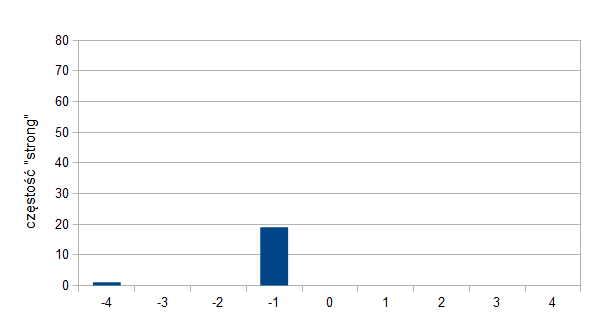
\includegraphics{charts/manning_shutze_160_1}
\caption
	[Słowo \emph{strong} w odniesieniu do słowa \emph{opposition}]
	{
		Słowo \emph{strong} w odniesieniu do słowa \emph{opposition} 
		\begin{displaymath}
			(\bar{d} = -1.15, s = 0.67)
		\end{displaymath}	
		na podstawie wykresów z \cite[str. 160]{mit}
	}
\label{manning_shutze_160_1}
\end{figure}

\par
Pierwszy z wykresów (\ref{manning_shutze_160_1}) składa się w zasadzie z pojedynczego, wysokiego piku, obrazującego, że większość wszystkich wystąpień słowa \emph{strong} razem z \emph{opposition} miało miejsce w odległości minus jeden, czyli słowa te występowały prawie zawsze po sobie w ustalonej kolejności, tworząc zwrot \emph{strong opposition}.
Dodatkowo według Manninga i Schütze wartość odchylenia standardowego jest niska i równa 0.67, a średnia odległość to -1.15 słowa.
Taki wynik, mimo dużego skupienia w okolicy argumentu minus jeden, został spowodowany szumem w danych -- pojedynczym wystąpieniem tej pary słów w odległości równej minus cztery wyrazy \cite[str. 159]{mit}.

\begin{figure}[h!]
\centering 
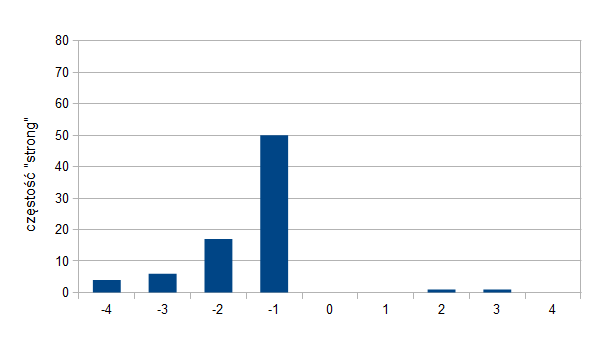
\includegraphics{charts/manning_shutze_160_2} 
\caption
	[Słowo \emph{strong} w odniesieniu do słowa \emph{support}]
	{
		Słowo \emph{strong} w odniesieniu do słowa \emph{support} 
		\begin{displaymath}
			(\bar{d} = -1.45, s = 1.07)
		\end{displaymath}	
		na podstawie wykresów z \cite[str. 160]{mit}
	}
\label{manning_shutze_160_2}
\end{figure}

\par
Na drugim z wykresów (\ref{manning_shutze_160_2}) zamieszczone zostały wyniki, z których wywnioskować można, że słowa \emph{strong} i \emph{support} występowały zazwyczaj w odległości minus jeden od siebie, ale wystąpiło także stosunkowo dużo sytuacji, w których ta odległość była większa, jednak prawie zawsze ujemna.
Zaobserwować można także niemal monotoniczny przebieg wykresu, przy pominięciu mało znaczących, pojedynczych wystąpień w odległościach dwa i trzy.
Zwiększenie zakresu argumentów, dla których występują znaczące wartości określające liczbę wystąpień miało wpływ na wzrost wartości wariancji do poziomu 1.07 \cite[str. 161]{mit}.

\begin{figure}[h!]
\centering
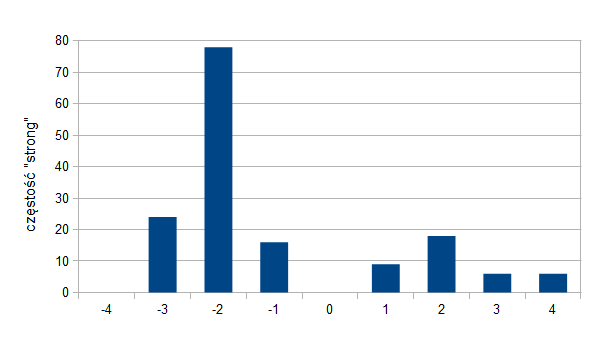
\includegraphics{charts/manning_shutze_160_3}
\caption
	[Słowo \emph{strong} w odniesieniu do słowa \emph{for}]
	{
		Słowo \emph{strong} w odniesieniu do słowa \emph{for} 
		\begin{displaymath}
			(\bar{d} = -1.12, s = 2.15)
		\end{displaymath}	
		na podstawie wykresów z \cite[str. 160]{mit}
	}
\label{manning_shutze_160_3}
\end{figure}

\par
Trzeci wykres (\ref{manning_shutze_160_3}) obrazuje wyniki dla zwrotu niebędącego kolokacją, składającego się z pary wyrazów \emph{strong} oraz \emph{for}.
Wartości na osi rzędnych dla różnych argumentów -- wartości odległości, osiągają znaczące poziomy, nie wykazując żadnej monotoniczności czy skoncentrowania w okolicy jednej z wartości odległości, jak to miało miejsce w przypadku dwóch poprzednich wykresów.
Mimo wysokiej wartości częstości wystąpień dla odległości równej minus dwa (duży pik), taki rozkład wyników spowodował znaczy wzrost wariancji w stosunku do rezultatów poprzednich badań -- odpowiednio ponad trzy- i dwukrotny.
Wysoka wartość wariancji i ocena rozkładu odległości rozpatrywanych wyrazów od siebie spowodowała odrzucenie kandydata \emph{strong for} jako interesującego w kontekście wyrażeń wielowyrazowych \cite[str. 161]{mit}.

\par
Interesującym zestawieniem wyników może być tabela \ref{mean_variance_result_table}, utworzona na podstawie danych z tabeli numer 5.5 w pracy \cite[str. 161]{mit}.
\begin{table}[h!]
\centering
\begin{tabular}{l l l | l | l}
	\toprule
	\textbf{s}	& \textbf{odległość}	& \textbf{częstość}	& \textbf{słowo A}		& \textbf{słowo B} 	\\
	\midrule
	0.43		& 0.97					& 11657				& New					& York				\\
	0.48 		& 1.83					& 24				& previous				& games				\\
	0.15 		& 2.98 					& 46				& minus					& points			\\
	0.49 		& 3.87 					& 131				& hundreds				& dollars			\\
	\midrule
	1.07 		& 1.45 					& 80				& strong				& support			\\
	1.13 		& 2.57 					& 7					& powerful				& organizations		\\
	1.01 		& 2.00 					& 112				& Richard				& Nixon				\\
	1.05 		& 0.00 					& 10				& Garrison				& said				\\
	\midrule
	4.03 		& 0.44 					& 36				& editorial				& Atlanta			\\
	4.03 		& 0.00 					& 78				& ring					& New				\\
	3.96 		& 0.19 					& 119				& point					& hundredth			\\
	3.96 		& 0.29 					& 106				& subscribers			& by				\\
	\bottomrule
\end{tabular}
\caption[Wyniki ekstrakcji kolokacji dla metody wariancji i odległości słów]{Wyniki ekstrakcji kolokacji z zastosowaniem metody opartej o wariancję i odległość słów \cite[str. 161]{mit}.}
\label{mean_variance_result_table}
\end{table}

Cztery pierwsze pozycje tabeli obrazują dobrych kandydatów na kolokacje, których cechuje niska wartość odchylenia standardowego.
Cztery ostatnie wiersze to nieinteresujące w kontekście jednostek wielowyrazowych wyrażenia -- ich odchylenie standardowe jest za wysokie, a dodatkowo średnia odległość wyrazów składowych od siebie jest bliska zeru.
Świadczy to o tym, że owe dwa słowa mogą występować w zasadzie w dowolnej kolejności lub szyku.
Natomiast cztery środkowe pozycje to wyrażenia, których wyrazy występowały w kilku różnych odległościach znaczącą liczbę razy \cite[str. 162]{mit} i są trudniejsze do jednoznacznej oceny niż poprzednie przypadki.


\subsection{Rozszerzenie metody o filtr pików}
Przedstawiona tutaj metoda średniej arytmetycznej i wariancji jest uproszczoną wersją techniki stosowanej przez Smajdę, który opisał ją w 1993 roku \cite{smadja_xtract}.
Wspomniany badacz używał dodatkowo filtru, który odrzucał kandydatów, dla których na wykresie pojawiał się tak zwany płaski pik.
Termin ten określa sytuację, gdy istnieje pewna wysoka wartość dla któregoś z argumentów, ale jednocześnie wartości dla argumentów z jego otoczenia także są znaczącymi liczbami.
Manning i Schütze jako przykład płaskiego piku podali trzeci z poprzednio omawianych wykresów (\ref{manning_shutze_160_3}), dotyczący pary słów \emph{strong for}. 


\subsection{Wyniki dla algorytmu po zastosowaniu filtru}
Przy zastosowaniu tego sposobu wydobywania kolokacji i omówionego filtrowania płaskich pików, Smajda osiągnął dokładność na poziomie osiemdziesięciu procent \cite[str. 162]{mit}.


\subsection{Wnioski}
Wizualizacja danych, tak jak wspomniano wcześniej, może być dodatkowym, pomocnym narzędziem przy ocenie kandydata na kolokację lub próbie wyznaczenia progu wartości wariancji, który będzie używany do odrzucania wyrażeń potencjalnie niebędących jednostkami wielowyrazowymi.
Mimo niewielkiego skomplikowania modelu statystycznego i prostoty filtru Smajda \cite{smadja_xtract} \cite[str. 162]{mit} pokazał, że metoda ta może być skuteczna, a dodatkowo pozwala na ekstrakcję kolokacji nieciągłych co nie było możliwe z wykorzystaniem przedstawionej we wcześniejszej części pracy metody zliczania.


\section{Funkcje asocjacyjne}
Pierwsze dwie omówione metody wykorzystywały częstości słów i konkretnych zestawów wyrazów do oceny wyrażeń w kontekście kandydatury na kolokacje.
Niestety występują trzy problemy związane z uwzględnianiem tylko surowej częstości tokenów w korpusie -- dwa zostały przytoczone przez Everta \cite[str. 20]{evert}, a trzeci przez Manninga i Schütze \cite[str. 162]{mit}.

\par
Pierwszy problem polega na tym, że częste współwystępowanie słów może być czystym przypadkiem, zwłaszcza jeśli częstość tych wyrazów w tekście jest wysoka. 
Fakt ten wpływa negatywnie na jakość oceny kandydatów na jednostki wielowyrazowe z wykorzystaniem metod opartych o zliczanie, więc istotne jest wprowadzanie interpretacji statystycznej częstości \cite[str. 20]{evert}.

\par
Drugi problem to wspomniana już wcześniej generalizacja dla całego języka na podstawie tylko danych wydobytych z pewnego korpusu.
Informacje wyekstrahowane z podzbioru tekstów danego języka, przykładowo tylko z pojedynczego korpusu, mogą okazać się niezrównoważone, niepełne, być jedynie zbliżonymi do tych, które są prawdziwe dla tego języka w ogólności.
Problem ten to ewentualna mała reprezentatywność wykorzystanych danych.

\par
Manning i Schütze zwrócili uwagę na trzeci problem związany z metodą zliczania opartą o odległość i wariancję.
Zauważyli, że wysoka częstość i niska wariancja współwystępowania słów mogą być przypadkowe w sytuacji, kiedy składowe wyrażenia występują często - wtedy oczekiwać można dużej liczby ich współwystąpień tylko ze względu na szansę na takie zdarzenie, a nie na poziom istotności tego wyrażenia w kontekście wydobywania kolokacji \cite[str. 162]{mit}.
Problem polega na tym, że oczekiwanym wynikiem jest informacja nie o tym, czy dany zestaw słów współwystępuje często, tylko czy współwystępuje częściej, niż wynika to jedynie z szansy na takie zdarzenie \cite[162]{mit}.

\par
Próbą rozwiązania wyszczególnionych problemów są różne modele statystyczne.
Mają one udzielać informacji, czy określone obserwacje współwystępowania bytów są czysto przypadkowe, wynikające po prostu z prawdopodobieństwa ich wystąpienia, czy faktycznie istnieją wystarczająco mocne przesłanki statystyczne do tego, aby stwierdzić, że powiązanie pomiędzy nimi faktycznie istnieje i jest istotne. 
Takimi szeroko stosowanymi metodami statystycznymi są \emph{funkcje asocjacyjne} zwane także \emph{miarami asocjacji}, za pomocą których można obliczyć \emph{miarę powiązania} pomiędzy argumentami zadanymi dla funkcji.
Dla przykładu w przypadku bi-gramów argumentami dla tych metod będą pary wyrazów rozważanego kandydata na wyrażenie wielowyrazowe.
Otrzymane za pomocą funkcji asocjacji wyniki, będące liczbami rzeczywistymi, określają stopień powiązania elementów -- to, jak nieprzypadkowe jest ich współwystąpienie. 
Dodatkowo wyniki te mogą posłużyć do utworzenia rankingu i dokonania selekcji kandydatów na kolokacje.

\par
Sytuacja, w której elementy współwystępują częściej niż gdyby były od siebie niezależne, określana jest mianem \emph{asocjacji pozytywnej}, a w przypadku przeciwnym, kiedy występują rzadziej, mianem \emph{asocjacji negatywnej}.
Z powyższym wiąże się ważna cecha funkcji asocjacyjnych w kontekście dostarczanych przez nie wyników -- przynależność do jednej z dwóch następujących grup: \emph{miar jednostronnych} albo \emph{miar dwustronnych}.
Pierwsza z grup zawiera te miary asocjacji, w przypadku których wysoki wynik oznacza silne powiązanie pozytywne, zaś niski -- brak wystarczającego dowodu na powiązanie pozytywne pomiędzy badanymi elementami.
Może występować powiązanie negatywne lub brak powiązania, ale nie da się tego określić na podstawie wyniku działania tej funkcji.
Druga z grup natomiast zawiera miary, których wysoka wartość oznacza silne powiązanie, ale nie daje informacji o tym, jakiego jest ono rodzaju -- pozytywne czy negatywne, a wynik o niskiej wartości to według tej funkcji słabe powiązanie pomiędzy elementami lub jego brak
\cite[str. 20, 21, 75, 76]{evert}.

\par
Większość metod statystycznych omawianych w tej części pracy korzysta z uproszczenia, polegającego na założeniu, że tekst to jedynie zbitka losowo występujących wyrazów ograniczonych przez zasady syntaktyczne języka \cite[str. 6]{pecina_measures}.
Tym samym szansa na wystąpienia danego słowa po dowolnym wyrazie poprzedzającym, nawet takim samym, jest zawsze identyczna na przestrzeni całego tekstu, jednak może być różna dla każdego ze słów.
Chociaż już w 1957 roku Firth zwrócił uwagę osób zajmujących się lingwistyką, że stwierdzenie to jest nieprawdziwe \cite[str. 15]{evert}, i tak jest ono wykorzystywane, niejednokrotnie z powodzeniem, w znacznej części niekontekstowych metod statystycznych, jakimi są miary asocjacyjne.

\par
Funkcje asocjacyjne stosowane są od przynajmniej pół wieku.
Już w roku 1965 dostępnych była pewna liczba funkcji asocjacyjnych, a przez kolejne prawie pięćdziesiąt lat powstało i zostało zbadanych wiele kolejnych. 
Jednak mimo dużej liczby tych miar niewiele z nich zyskało dużą popularność.
Do najbardziej znanych należą \emph{MI (Mutual Information)}, \emph{T-score}, \emph{Log-likelihood} oraz $ Chi^2 $ \cite[str. 21]{evert}.

\par
Pavel Pecina w swoich pracach przedstawił dziesiątki miar asocjacyjnych \cite[str. 3]{coling}\cite[str. 18]{pecina_measures}.
Wszystkie zostały podzielone na sześć grup \cite[str. 2]{coling} -- stanowią one sześć pierwszych pozycji na poniższej liście.
Dodatkowo wyróżnić można kolejne dwie grupy metod ekstrakcji kolokacji -- dwie ostatnie pozycje na liście.

\begin{enumerate}
	\item estymacje współwystąpienia i prawdopodobieństwa warunkowego;
	\item \emph{Mutal Information} i jej pochodne;
	\item testy statystyczne niezależności;
	\item miary z rodziny \emph{likelihood};
	\item zestaw heurystycznych miar asocjacyjnych oraz współczynników zależności;
	\item miary kontekstowe;
	\item \emph{miary mieszane};
	\item \emph{uczenie maszynowe};
\end{enumerate}

Grupy te wraz z przykładami zostały omówione w kolejnych częściach tej sekcji.
Przed ich preyentacjA należy jednak zdefiniować oznaczenia używane we wzorach opisujących te miary:

\begin{itemize}
	\item $ x $ - element \emph{x};
	\item $ \bar{x} $ - element inny niż \emph{x};
	\item $ (x, y, ...) $ - zbiór elementów \emph{x}, \emph{y}, \ldots;
	\item $ p(x) $ - prawdopodobieństwo wystąpienia elementu \emph{x};
	\item $ f(x) $ - częstość elementu \emph{x}, zaobserwowana w zbiorze danych;
	\item $ \hat{f}(x) $ - wartość oczekiwana elementu \emph{x}.
\end{itemize}


\subsection{Współwystąpienia i prawdopodobieństwo warunkowe}
Pierwsza z grup zawiera w sobie trzy podstawowe miary: prawdopodobieństwo współwystąpienia $ p(x, y) $, prawdopodobieństwo warunkowe $ p(x|y) $ oraz odwrócone prawdopodobieństwo warunkowe $ p(y|x) $.
Przytoczone miary to podstawa wykorzystywana w kolejnych rodzinach miar asocjacji.

\subsection{Miary informacji}
Jedną z najpopularniejszych funkcji asocjacyjnych, będących miarą informacji, jest \emph{Mutual Information} wyrażona wzorem\cite[str. 2]{mmi_w11}:

\begin{center}
\( I(X; Y) = \sum_{x \in X} \sum_{y \in Y} p(x, y) log_{2} \frac{p(x, y)}{p(x) * p(y)} \)
\end{center}

Miara ta oblicza ile informacji w jednej zmiennej losowej \emph{X} jest jednoczenie zawarte w drugiej zmiennej losowej \emph{Y} \cite[str. 2]{mmi_w11}.
Natomiast miara \emph{Pointwise Mutual Information} jest wykorzystana do obliczenia poziomu asocjacji dwóch konkretnych wartości zmiennych losowych \emph{X} i \emph{Y}.
Funkcja \emph{PMI} \cite[str. 2]{mmi_w11}, szeroko wykorzystywana w badaniach nad wydobywaniem kolokacji, wyrażona jest wzorem:

\begin{center}
\( pmi(x, y) = log_{2} \frac{p(x, y)}{p(x) * p(y)} \)
\end{center}

Obie z przytoczonych funkcji zostały wykorzystane do budowy innych miar informacji wykorzystywanych w wydobywaniu jednostek wielowyrazowych.


\subsection{Testy statystyczne niezależności}
Jako przykłady miar należących do tej grupy autor niniejszej pracy wybrał trzy: \emph{T-score}, \emph{Z-score} oraz $ Pearson's $ $ X^2 $.
\par
Pierwsza z nich jest częścią \emph{T-testu} \cite[str. 166]{mit}, który składa się trzech głównych kroków: obliczenia wartości dla testu, ustalenia progu wiarygodności i wykonania testu. 
\emph{T-score} natomiast składa się z jednego punktu i jest wykorzystana do tworzenia rankingu, wyliczania wartości zamiast klasyfikacji obserwacji.
Miara \emph{T-score} jest nazywana w literaturze mianem \emph{T-testu} \cite[str. 3]{coling}\cite[str. 18]{pecina_measures}, jednak ze względu na to, że jest jedynie jego częścią polegającą na wyliczeniu wartości, którą można wykorzystać w \emph{T-teście}, w niniejszej pracy będzie nazywana \emph{T-score}.
Wartość tej miary obliczyć można wykorzystując następujący wzór \cite[str. 18]{pecina_measures}:

$$ \frac{f(x, y) - \hat{f}(x, y) }{\sqrt{f(x, y) * (1 - (f(x, y) / N))}} $$

\par
Druga z miar to \emph{Z-score}, która także służy do wyliczenia wartości rankingowej obserwacji, a nie klasyfikacji.
Miara ta w dwóch wcześniej wspomnianych pracach \cite[str. 3]{coling}\cite[str. 18]{pecina_measures} nazywana została już \emph{score}, a nie \emph{test}, jak w przypadku \emph{T-Score}.
Opisana jest za pomocą poniższego wzoru \cite[str. 18]{pecina_measures}:

$$ \frac{f(x, y) - \hat{f}(x, y) }{\sqrt{\hat{f}(x, y) * (1 - (\hat{f}(x, y) / N))}} $$

Różnica pomiędzy miarami \emph{T-score} a \emph{Z-score} to wykorzystanie wartości oczekiwanej zamiast zaobserwowanej w mianowniku wzoru.
Obie te funkcje jednak mają ważną cechę wspólną -- zakładają, że rozkład prawdopodobieństwa w zbiorze danych jest rozkładem normalnym, co w znacznej części przypadków praktycznych nie jest prawdziwe \cite[str. 169]{mit}.

\par
Trzecia z miar to $ Pearson's $ $ X^2 $.
Jej zaletą w stosunku do dwóch poprzednich jest brak założenia co do rozkładu normalnego prawdopodobieństwa w zbiorze danych.
Zamiast tego test zakłada rozkład $ X^2 $ ($ Chi^2 $), który powinien być bardziej odpowiedni do realizacji zadania ekstrakcji kolokacji.
Miara korzysta z tablicy wielodzielnej (ang. contingency table) \cite[str. 169]{mit} w celu porównania wartości obserwowanych z oczekiwanymi i na tej podstawie oceny, czy hipoteza zerowa może zostać odrzucona, a niezerowa przyjęta za prawdziwą.
$ Pearson's $ $ X^2 $ w niniejszej pracy oraz w pracach Pavla Peciny została wykorzystana jako funkcja rankingowa.
Dokonano tego analogicznie jak w przypadku \emph{T-testu}, wyliczono jedynie wartość dla testu, ale on sam nie został wykonany, a uzyskana wartość służy jako wyznacznik pozycji w rankingu.
Wzór funkcji jest następujący \cite[str. 18]{pecina_measures}:

$$ \sum_{i, j} \frac{(f_{i, j} - \hat{f}_{i, j})^{2}}{\hat{f}_{i, j}} $$


\subsection{Funkcje z rodziny \protect\textit{likelihood}}
Dwie funkcje z rodziny \emph{likelihood} zostały zaprezentowanych i zbadane w pracach Pavla Peciny \cite[str. 3]{coling}.
Pierwsza z nich została nazwana \emph{Log likelihood ratio} i została zapisana w formie wzoru:

$$ -2 \sum_{i, j} f_{i, j} log \frac{f_{i, j}}{\hat{f}_{i, j}} $$

Druga funkcja jest modyfikacją pierwszej, jest pozbawiona jednego członu i wyrażona wzorem:

$$ -2 \sum_{i, j} \frac{f_{i, j}^2}{\hat{f}_{i, j}} $$

Według Manninga i Schütze \cite[str. 172]{mit} miary z rodziny \emph{likelihood} są lepsze od testów $ Chi^2 $ dla danych rzadkich, jakimi są kolokacje w dużych zbiorach tekstowych. 
Dodatkowo wyniki są bardziej interpretowalne, ponieważ wskazują czy jedna z hipotez jest bardziej prawdopodobna od drugiej.


\subsection{Miary kontekstowe}
Pavel Pecina w swoich pracach \cite[str. 18]{pecina_measures}\cite[str. 3]{coling} prezentuje 24 miary kontekstowe, których jakość także bada.
Miary kontekstowe bazują na kontekstach (otoczeniu) słów i kandydatów na kolokacje.
Wykorzystywane w przedstawionych przez Pavla Pecine miarach są konteksty dwu- oraz jednostronne i na ich podstawie oraz z wykorzystaniem danych o częstościach obliczane są wartości rankingowe.
Miary kontekstowe wykorzystują także informacje pochodzące z otoczenia kandydatów na wyrażenia wielowyrazowe, a nie tylko dane dotyczące ich bezpośrednio (ich częstości).
\par
Praca Peciny i Schlesingera \cite[str. 4]{coling} wskazuje na to, że miara kontekstowa o nazwie \emph{Cosine context similarity in boolean vector space} osiągnęła jeden z dwóch najlepszych wyników spośród wszystkich osiemdziesięciu dwóch sprawdzonych przez Pecinę i Schlesingera funkcji \cite[str. 4]{coling}.
Obrazuje to, że kontekst może być bardzo pomocny przy ocenie kandydatów na kolokacje.


\subsection{Miary mieszane}
Podejście miar mieszanych zostało zaczerpnięte z prac Peciny i Schlesingera \cite{coling} oraz Anca Dinu, Liviu P. Dinu, Ionut T. Sorodoc \cite{aggregation}.
Pomysł przedstawiony w drugiej z prac polega na wygenerowaniu zestawu rankingów dla różnych miar asocjacyjnych, a następnie opcjonalnym wykonaniu ich przepunktowania, polegającego na zachowaniu kolejności w rankingu, ale zmianie wartości dla każdej z pozycji.
Przykładowymi miarami przepunktowania rankingów są \emph{Rank distance} i \emph{Borda score} \cite[str. 2]{aggregation}.
Kiedy rankingi są gotowe należy poddać je agregacji w celu wygenerowania pojedynczego, finalnego rankingu, który jest także wynikiem algorytmu.
\par
Pavel Pecina wykorzystuje natomiast miary mieszane w innym celu -- opisanym w podrozdziale 3.3.8.


\subsection{Uczenie maszynowe}
Praca Peciny i Schlesingera \cite{coling} pokazuje sposób na wykorzystanie miar asocjacyjnych w celu wygenerowania cech dla algorytmów maszynowego uczenia i regresji liniowej.
\par
Proces generowania cech ma trzy krotki.
Pierwszy z nich to dobór miar asocjacyjnych, które zostaną wykorzystane jako składowe generatora cech do wykorzystania w procesie maszynowego uczenia.
Pavel Pecina wskazuje \cite{coling}, że jest to krok istotny, ze względu na to, iż wiele miar dzieli ze sobą w części te same informacje, a tym samym wykorzystanie niektórych z nich nie powoduje uzyskania dużo lepszych wyników.
Badacz pokazał, że można osiągnąć podobne jakościowo wyniki redukując liczbę dobranych miar asocjacyjnych z 82 do 17 przy zachowaniu około 95\% ich całkowitej wariancji.
Z kolei jedynie 42 miar powoduje utrzymanie poziomu w okolicy 99.9\% \cite[str. 7]{coling}.
Dodatkowo Mariusz Paradowski w swojej pracy \cite{paradowski_beta} zbadał część funkcji asocjacyjnych i wykazał, które z nich są ze sobą skorelowane i w efekcie generują równoważne rankingi.
Polega to na zachowaniu takiej samej kolejności pozycji w różnych rankingach, ale przy ewentualnej różnicy oceny danych bytów na poszczególnych pozycjach.
Informacje te mogą posłużyć do lepszego doboru miar w procesie tworzenia cech dla algorytmów maszynowego uczenia.

\par
Drugi krok generacji cech polega na wykorzystaniu miar asocjacyjnych dla każdego badanego kandydata na kolokacje.
Efektem tego działania jest jeden wektor dla każdej krotki, a każda pozycja tego wektora przechowuje wynik jednej z funkcji asocjacyjnych.
Dodatkowo jeden z jego elementów przechowuje informację, o tym czy kandydat jest kolokacją czy nie -- informacja ta jest wykorzystywana w procesie uczenia nadzorowanego.
W pracy Peciny i Schlesingera klasa jest dwuwartościowa, ale wydaje się, że nic nie stoi na przeszkodzie, aby przypisać jej więcej możliwych wartości.
Przykład wektora został zamieszczony poniżej:
$$ wektor\_cech = [x_{1}, x_{2}, ..., x_{n}, klasa], gdzie: $$
\begin{enumerate}
	\item $ x_{i} $ - wynik dla miary \emph{i};
	\item $ klasa $ - klasa kandydata na wyrażenie wielowyrazowe\end{enumerate}.
\par
Trzeci krok jest opcjonalny i polega na przetworzeniu otrzymanych cech.
Przykładowym algorytmem wykorzystanym w tym celu może być zwykła \emph{normalizacja} lub jak w pracy \cite[str. 6]{coling} - \emph{standaryzacja}.

\par
Po wykonaniu dwóch pierwszych i ewentualnie trzeciego kroku cechy są gotowe do wykorzystania ich w procesie uczenia maszynowego i klasyfikacji.
Pavel Pecina użył tak wygenerowanych cech do uczenia klasyfikatorów, takich jak jednowarstwowa sztuczna sieć neuronowa czy \emph{Support Vector Machine}.
Wyniki przedstawione w jego pracy \cite[str. 7]{coling} są obiecujące i wskazują, że metody maszynowego uczenia mogą okazać się znacząco lepsze od samych funkcji asocjacyjnych.


\section{Ekstrakcja kolokacji tri-gramowych i dłuższych}
Ekstrakcja wyrażeń wieloelementowych składających się z trzech lub więcej wyrazów jest procesem bardziej złożonym obliczeniowo i trudniejszym koncepcyjnie niż wyszukiwanie kolokacji dwuelementowych.
Wiele podejść do wydobywania wyrażeń trzy- oraz więcej elementowych opierało się na dokonaniu generalizacji metod wykorzystywanych do ekstrakcji par słów lub wykorzystaniu specjalnie do tego przygotowanych miar heurystycznych.


\subsection{Rozszerzenie miary \emph{Mutual Information}}
Praca Tima Van de Cruys \cite{mmi_w11} jest poświęcona rozważaniom nad dwoma alternatywnymi wersjami generalizacji funkcji \emph{Mutual Information}.
Pierwsza z nich bazuje na mierze \emph{Interaction Information} wyrażanej wzorem \cite[str. 2]{mmi_w11}:
$$ I(X; Y| Z) = \sum_{x \in X} \sum_{y \in Y} \sum_{z \in Z} p(x, y, z) log \frac{p(x, y| z)}{p(x| z)p(y| z)} $$

Na podstawie tej miary Tim Van de Cruys zaproponował rozszerzenie funkcji \emph{Mutual Information} do postaci uwzględniającej trzy zmienne losowe zamiast dwóch \cite[str. 2]{mmi_w11}:
$$ I(X; Y; Z) = I(X; Y| Z) - I(X; Y) = I(X; Z| Y) - I(X; Z) = I(Y; Z| X) - I(Y; Z) $$

Rozszerzona wersja pierwszego z powyższych przypadków ma zatem postać \cite[str. 2]{mmi_w11}:
$$ I(X; Y; Z) = \sum_{x \in X} \sum_{y \in Y} \sum_{z \in Z} p(x, y, z) log \frac{p(x, y, z)p(z)}{p(x, z)p(y, z)} - \sum_{x \in X} \sum_{y \in Y} p(x, y) log \frac{p(x, y)}{p(x)p(y)} $$

Odpowiednikiem miary \emph{Pointwise Mutual Information} dla \emph{Interaction Information} jest funkcja \emph{Specific Interaction Information} \cite[str. 2]{mmi_w11}, a jej wzór jest następujący \cite[str. 3]{mmi_w11}:
$$ SI(x, y, z) = log \frac{p(x, y)}{p(x)p(y)} - log \frac{p(x, y, z)p(z)}{p(x, z)p(y, z)} = log \frac{p(x, y)p(y, z)p(x, z)}{p(x)p(y)p(z)p(x, y, z)} $$

\par
Tim Van de Cruys w swoim artykule przedstawił także jeszcze jedną wersję generalizacji \emph{Mutual Information} \cite{mmi_w11}.
Miara zwana \emph{Total Correlation} lub \emph{Multi-Information} bada ilość informacji współdzielonych pomiędzy zmiennymi losowymi z pewnego ich zbioru \cite[str. 3]{mmi_w11}.
Jej zaletą jest prosta generalizacja do dowolnej liczby zmiennych losowych, stosunkowo niska złożoność wzoru w porównaniu z poprzednią propozycją, a dodatkowo miara ta była używana w zadaniach przetwarzania języka naturalnego przy ekstrakcji kolokacji \cite[str. 3]{mmi_w11}.
Funkcja została przedstawiona w pracy Watanabe w roku 1960 i opisana za pomocą poniższego wzoru \cite[str. 3]{mmi_w11}:
$$ I(X_{1}, X_{2}, ..., X_{n}) = \sum_{x_{1} \in X_{1}, x_{2} \in X_{2}, ...,  x_{n} \in X_{n}} p(x_{1}, x_{2}, ..., x_{n}) log \frac{p(x_{1}, x_{2}, ..., x_{n})}{\sqcap_{i=1}^{n} p(x_{i})} $$

Wersja miary \emph{Total Correlation} analogiczna do dwuargumentowego \emph{Pointwise Mutual Information} nazwana \emph{Specific Correlation} wyraża się następującym wzorem \cite[str. 3]{mmi_w11}:
$$ SI(x_{1}, x_{2}, ..., x_{n}) = log \frac{p(x_{1}, x_{2}, ..., x_{n})}{\sqcap_{i=1}^{n}p(x_{i})} $$

\par
Dwie przedstawione miary, będące rozszerzeniem \emph{Mutual Information} są przykładami podejścia wykorzystującego generalizację miar działających na parach argumentów w celu wykorzystania ich do obliczeń na większej liczbie parametrów.


\subsection{Wyniki dla miar \emph{Interaction Information} oraz \emph{Total Correlation}}
Tim Van de Cruys w artykule \cite{mmi_w11} badał wydobywanie jednostek trójelementowych postaci \emph{subject, verb, object} z wykorzystaniem obu przedstawionych tutaj generalizacji \emph{Mutual Information} oraz za pomocą zwykłego rankingu częstości wystąpień \cite[str. 4]{mmi_w11}.
Według jego wyników zamieszczonych dla zadanych zbiorów danych lepsza okazała się prostsza wersja generalizacji miary \emph{Mutual Information} -- \emph{Specific Correlation}.
Wyniki przytoczone z tej pracy zostały zamieszczone w poniższej tabeli \ref{mmi_results}\footnote{Dane na podstawie wyników pracy zamieszczonych w \cite[str. 4]{mmi_w11}.}:

\begin{table}[h!]
\centering
\begin{tabular}{l | l}
	\toprule
	\textbf{miara} 							& \textbf{precyzja}	\\
	\midrule
	częstości								& 0.00				\\
	\emph{Specific Interaction Information}	& 0.24				\\
	\emph{Specific Correlation}				& 0.31				\\
	\bottomrule
\end{tabular}
\caption
	[Wyniki badań dwóch generalizacji funkcji \emph{Mutual Information}.]
	{Wyniki badań dwóch generalizacji funkcji \emph{Mutual Information} zaczerpnięte z \cite[str. 4]{mmi_w11}.}
\label{mmi_results}
\end{table}
Różnica w dokładności wyników pomiędzy dwoma przedstawionymi funkcjami jest według Tima Van de Cruysa wartością znaczącą \cite[str. 5]{mmi_w11}.
Ponadto, obie z tych miar spisały się nieporównywalnie lepiej niż zwykłe wybieranie wyrażeń o najwyższej częstości \cite[str. 5]{mmi_w11}, co może świadczyć o zasadności użycia opisanych funkcji i ich przydatności.
Zamieszczone wyniki zdają się być dobrymi przesłankami do wykorzystania opisanych miar asocjacyjnych w badaniach.


\subsection{Heurystyki generalizujące miary dwuelementowe}
Sasa Petrovic, Jan Snajder, Bojana Dalbelo Basic w swoim artykule \cite{generalization_patterns} zebrali istniejące, a także zaproponowali nowe wzorce budowy funkcji heurystycznych do wydobywania kolokacji dłuższych niż dwuelementowe.
Opisane przez nich wzorce podchodzą do problemu w podobny sposób -- rozbijają kolokacje N-elementowe na zestaw kolokacji 2-elementowych, ale robią to inną metodą; wyjątkiem jest pierwsza z miara oznaczona \( G_{0} \).
Każda z sześciu kolejnych metod po podzieleniu N-elementowej krotki ocenia wszystkie powstałe bi-gramy, wykorzystując do tego dwuelementową funkcję asocjacyjną (przykładowo jedną z zaprezentowanych wcześniej -- \emph{Pointwise Mutual Information}).
Następnie, na podstawie zestawu wyników, dokonuje ich przetworzenia w pojedynczą wartość.
Praca zawiera opis siedmiu wzorców generalizacji miar dwuelementowych.

\par
Pierwszym przykładem jest wzorzec \( G_{0} \), który wyróżnia się podejściem na tle pozostałych metod.
Zakłada on intuicyjną generalizację już istniejących metod.
Autorzy pracy podali dwa przykłady dla funkcji \emph{Pointwise Mutual Information} i \emph{Dice} \cite[str. 4]{generalization_patterns}.
Wzory zostały zamieszczone poniżej:
$$ G_{0}(PMI, x_{1} ... x_{n}) = log_{2} \frac{P(x_{1} ... x_{n})}{\prod_{i = 1}^{n} P(x_{i})} $$

$$ G_{0}(Dice, x_{1} ... x_{n}) = \frac{nf(x_{1} ... x_{n})}{\sum_{i = 1}^{n} f(x_{i})}, gdzie: $$

\begin{enumerate}
	\item $ x_{i} $ - i-ta składowa N-elementowej krotki;
	\item $ x_{1} ... x_{n} $ - krotka N-elementowa;
	\item $ n $ - liczba elementów krotki.
\end{enumerate}

\par
Drugim przykładem miary dokonującej podziału jest \emph{Average Bi-gram}, oznaczona jako $ G_{3} $ \cite[str. 5]{generalization_patterns} i opisana wzorem:
$$ G_{3}(x_{1} ... x_{n}) = \frac{1}{n - 1} \sum_{i = 1}^{n-1} FA(x_{i}, x_{i + 1}), gdzie: $$

\begin{enumerate}
	\item \( FA(x_{i}, x_{i + 1}) \) - wynik funkcji asocjacyjnej dla elementów \( x_{i} \) oraz \( x_{i + 1} \).
\end{enumerate}

\par
Trzeci przykład jest bardziej skomplikowany i został oznaczony jako $ G_{6} $ \cite[str. 5]{generalization_patterns}, a przez autora niniejszej pracy nazwany \emph{Smoothed Bi-gram}.
Wzorzec dzieli N-elementową krotkę na zestaw N-1 dwuelementowych krotek taki, że:
$$ krotka(x_{1}, x_{2}, ..., x_{n}) \rightarrow \{krotka(x_{1}, x_{2}), krotka(x_{2}, x_{3}), ..., krotka(x_{n - 1}, x_{n})\} $$

Po takim podziale wykorzystuje się inny wzorzec generalizacji, gdzie argumentami są wszystkie krotki powstałe poprzez podział opisany w poprzednim kroku, a ich częstości są równe liczbie wystąpień tych właśnie krotek 2-elementowych w zbiorze danych.
Dodatkowo, według autorów, wewnętrzną funkcją asocjacyjną dla wzorca wewnętrznego \( G_{0} \) jest miara wykorzystana we wzorcu zewnętrznym \( G_{6} \) \cite[str. 5]{generalization_patterns}.
Wydaje się jednak, że nic nie stoi na przeszkodzie, aby wykorzystać inny wzorzec wewnętrzny niż \( G_{0} \) oraz różne miary asocjacji w obu wzorcach - wewnętrznym i zewnętrznym.
Formalnie wzór dla tego wzorca przyjmuje następującą postać:
$$ G_{6}(AF, x_{1} ... x_{n}) = G_{0}(FA, (x_{1}x_{2}, x_{2}x_{3}, ..., x_{n - 1}x_{n})) $$

\par
Dodatkowo Mariusz Paradowski opracował miarę \emph{Minimalnego Bi-gramu}, która także rozbija kolokacje na zestaw krotek 2-elementowych.
Ocena kolokacji jest równa minimum z ocen wszystkich kolejnych, ciągłych i zachodzących na siebie bi-gramów.
Wzór miary prezentuje się następująco:
$$ ocena = min(s \forall s \in S : S = {FA(b) \forall b \in t}), gdzie: $$

\begin{enumerate}
	\item \emph{t} - krotka N-elementowa;
	\item \emph{b} - bi-gram utworzony z fragmentu N-elementowej krotki;
	\item \emph{FA(b)} - wynik funkcji asocjacyjnej dla bi-gramu.
\end{enumerate}


\subsection{Podsumowanie}
Literatura okazuje się być bogata w opisy, prezentacje, badania i porównania wielu różnych funkcji asocjacyjnych oraz innych sposobów wydobywania kolokacji dwuelementowych z tekstów.
Znaleźć można też różne sposoby i podejścia do zagadnienia ekstrakcji kolokacji dłuższych niż dwuelementowe.
Skrupulatny i szeroki przegląd literatury może być dobrą bazą do wykonywania kolejnych badań i testów metod ekstrakcji wyrażeń wieloelementowych z korpusów tekstowych.


\chapter{Narzędzie i oprogramowanie wykorzystane na potrzeby realizacji tematu}


\section{Biblioteka \protect\textit{Corpus2}}
Biblioteka \emph{Corpus2} \cite{corpus2_web} to zestaw struktur danych i funkcji do przetwarzania korpusów oznaczonych morfosyntaktycznie, z tagsetem pozycyjnym. 
Umożliwia ona wczytywanie i zapisywanie danych do różnych formatów danych takich jak \emph{XCES}, jego rozszerzeniem \emph{CCL} \cite{ccl_web} czy formatów tekstowo-tabelarycznych, takich jak \emph{IOB-Chan} \cite{iob_chan_web}.
Opcjonalnie biblioteka wspiera także pracę, wczytywanie danych, z binarnym i zindeksowanym formatem \emph{Poliqarp} \cite{korpus_ipi_pan} autorstwa pracowników Instytutu Podstaw Informatyki Polskiej Akademii Nauk, a opracowanym w celu przechowywania korpusów tekstowych.
Warto nadmienić, że biblioteka \emph{Corpus2} wspiera także wiele innych formatów plików.

\par 
Biblioteka została zaimplementowana w Instytucie Informatyki Politechniki Wrocławskiej w języku \emph{C++}, ale powstały także skrypty w języku Python, opakowania, umożliwiające pracę z tą biblioteką z wykorzystaniem tego właśnie języka skryptowego.
Dodatkowo narzędzie jest dostępne nieodpłatnie na licencji \emph{GNU LGPL 3.0} lub w przypadku wykorzystania formatu \emph{Poliqarp} na licencji GNU GPL 3.0 \cite{corpus2_web}.

\par
\emph{Corpus2} został wykorzystany w badaniach na potrzeby niniejszej pracy do wczytywania oznaczonych korpusów tekstowych z formatów \emph{IOB-Chan}, \emph{CCL}, a także \emph{Poliqarp}, a także do konwersji pomiędzy nimi.
Ponadto inne narzędzia wykorzystane w tej pracy także wykorzystują funkcjonalność tej biblioteki.


\section{Tagery \protect\textit{WCRFT} i \protect\textit{WCRFT2}}
Nazwa \emph{WCRFT} \cite{wcrft_web} jest akronimem powstałym od słów \emph{Wrocław Conditional Random Fields Tagger} - wrocławskie narzędzie tagujące oparte o model matematyczny \emph{Conditional Random Field}.
\emph{WCRFT} został zaimplementowany z myślą o oznaczaniu tekstów języków fleksyjnych, zwłaszcza słowiańskich, a szczególnie języka polskiego.

\par
Tager napisano w języku Python, z wykorzystaniem gotowej implementacji \emph{CRF} o nazwie \emph{CRF++}, która to napisana została w języku \emph{C++} \cite{wcrft}.
Narzędzie \emph{WCRFT} było implementowane głównie przez Adama Radziszewskiego.

\par
\emph{WCRFT2} natomiast jest następcą tagera \emph{WCRFT}.
Został on napisany całkowicie w języku \emph{C++} -- zostało dokonane portowanie kodu z języka Python do języka \emph{C++}.
Taki zabieg pozwolił na usunięcie zależności związanych z językiem skryptowym, znaczne przyspiesznie tagera (trzykrotne), a także usprawnił i ułatwił proces budowy narzędzia.
Zaznaczyć trzeba, że po wykonaniu konwersji pomiędzy językami zachowano kompatybilność modeli z poprzednią wersją tagera, a wyniki dla obu wersji są takie same.
Ta wersja jest teraz zalecaną do użycia, a poprzednia nie jest już wspierana.

\par
Narzędzie to, w celach badawczych wyszczególnionych w tej pracy, zostało wykorzystane do oznaczenia morfosyntaktycznego słów z zebranych tekstów języka polskiego, które następnie zostały wykorzystane w procesie badania sposobów ekstrakcji kolokacji.
Do wykonania prac wykorzystany został nowy, gotowy model dla tagera udostępniony przez grupę G4.19.

\section{Formalizm \protect\textit{WCCL}}
\subsection{Wyjaśnienie terminu}
\emph{WCCL (Wrocław Corpus Constraint Language)} \cite{wccl_web} jest formalizmem, językiem ograniczeń i narzędziem pozwalającym tworzyć wyrażenia funkcyjne, które można wykorzystać jako cechy (kluczowe informacje), dla wielu algorytmów przetwarzania języka naturalnego i maszynowego uczenia \cite{wccl}. 
Wyrażenia \emph{WCCL} działają na tekście uprzednio oznakowanym morfosyntaktycznie, na przykład za pomocą narzędzia wspomnianego we wcześniejszej części tej pracy -- tagera \emph{WCRFT2}. 
Chociaż formalizm ten był konstruowany z myślą o pracy z językiem polskim, według autorów powinien on także móc być użyty do pracy z innymi językami fleksyjnymi. 
Ograniczeniami mogą być jednak przyjęta tekstowa reprezentacja tagów oraz formaty oznakowanych korpusów, na których miałyby pracować wyrażenia \emph{WCCL} \cite[str. 1]{wccl}.

\par
Omawiany język ograniczeń został zaimplementowany w języku \emph{C++} w postaci bibliotek wykorzystujących \emph{Corpus2} oraz system \emph{MACA (Morphological Analysis Converter and Aggregator)}. 
Dodatkowo napisane zostały także skrypty w języku Python opakowujące funkcjonalność \emph{WCCL} i umożliwiające prace z poziomu języka skryptowego, bez konieczności zaznajomienia się z językiem natywnym, w jakim formalizm ten został zaimplementowany. 
Dzięki temu tworzenie narzędzi i praca z \emph{WCCL} może być szybsza i prostsza \cite[str. 3]{wccl}.

\par
Formalizm \emph{WCCL} został wykorzystany w badaniach z poziomu języka \emph{C++}, bez użycia opakowań, i posłuży głównie do filtrowania kandydatów na jednostki wielowyrazowe na podstawie weryfikacji, jakimi częściami mowy są składowe wyrażenia wielowyrazowego oraz w oparciu o inne cechy, takie jak przykładowo uzgodnienie rzeczownika z przymiotnikiem.
Autor niniejszej pracy zajął się badaniami nad kolokacjami w języku polskim, co rozwiązało ewentualne problemy mogące się pojawić przy pracy z innymi językami fleksyjnymi.

\subsection{Przykładowe wyrażenie}
Przykładowy, prosty operator \emph{WCCL} zbliżony swoją składnią do jednego z operatorów stosowanych w badaniach przeprowadzonych przez autora tej pracy zamieszczono poniżej. 

\begin{lstlisting}[frame=single, tabsize=2, language=Python, caption=Przykładowe wyrażenie w języku \emph{WCCL}, captionpos=b, breaklines=true, basicstyle=\scriptsize]
@b:"SubstAdjOrSubstSubst"
(
	or
	(
		and
		(
			inter(class[0], {subst}),
			inter(class[1], {adj, subst}),
		
			setvar($Case, 0)
		),
		and
		(
			inter(class[1], {subst}),
			inter(class[0], {adj, subst}),
		
			setvar($Case, 1)
		)
	)
)
\end{lstlisting}

Powyższy listing prezentuje kod wyrażenia w języku \emph{WCCL}.
Składa się on z dwóch części - nagłówka i ciała.
Istotną informacją jest fakt, że operator \emph{WCCL} jest kontekstowy, wywoływany jest dla konkretnego miejsca w korpusie, jakiegoś wyrazu w nim zawartego.
Wyraz ten nazwijmy \emph{początkiem kontekstu operatora}.

\par
Nagłówek zawiera dwie informacje o wyrażeniu.
Pierwsza z nich, \emph{@b}, to typ zwracany przez ten operator na podstawie wykonania instrukcji zawartych w jego ciele. 
Druga informacja to nazwa wyrażenia znajdująca się po dwukropku, tutaj będzie to \emph{SubstAdjOrSubstSubst}.
Powyższy kod zwróci jedną z dwóch wartości logicznych - \emph{True} lub \emph{False}.
Inne typy, które mogą zwracać operatory \emph{WCCL} to \emph{Position}, \emph{Set of strings} oraz \emph{Tagset symbol set}.
Pierwszy z nich to wartość całkowita - odpowiednik typu \emph{int} w języku \emph{C++}, drugi typ jest rozumiany jako zbiór ciągów znaków tekstowych, a trzeci to zestaw symboli używanego tagsetu.

\par
Przed opisem ciała powyższego przykładowego operatora należy wyjaśnić funkcje w nim użyte.
Pierwsze dwie z nich są intuicyjne - funkcja \emph{or} i \emph{and}.
Obie z nich zachowują się jak funkcje logiczne o tych samych nazwach anglojęzycznych, a argumenty dla nich są oddzielone przecinkiem tak samo jak w każdej funkcji języka \emph{WCCL}.
Funkcja \emph{setvar} ustawia wartość zmiennej o nazwie podanej w pierwszym argumencie na wartość zadaną parametrem drugim.
Natomiast funkcja \emph{inter} sprawdza przecięcie zbiorów zadanych jej argumentami i zwraca \emph{True} jeśli moc przecięcia jest niezerowa.
Kluczowa w tym wyrażeniu jest także funkcja \emph{class} przyjmująca tylko jeden argument typu całkowitego.
Funkcja ta zwróci klasę gramatyczną słowa oddalonego o zadaną argumentem liczbę wyrazów od \emph{początku kontekstu} tego wyrażenia.
Przykładowo przyjmijmy, że jakiś operator wywołuje kolejno funkcje \emph{class[-1]}, \emph{class[0]} i \emph{class[1]} na poniższym zdaniu, gdzie słowo będące \emph{początkiem kontekstu operatora} zostało oznaczone pogrubioną czcionką:
\begin{center}
Długie, ciężkie \textbf{spodnie} jeszcze się suszą.
\end{center}
Pierwsza funkcja z argumentem równym minus jeden zwróci klasę gramatyczną słowa \emph{ciężkie} czyli przymiotnik, druga klasę wyrazu będącego początkiem kontekstu operatora - \emph{spodnie}, czyli rzeczownik, natomiast wynikiem działania trzeciej dla wyrazu \emph{jeszcze} będzie partykuła.

\par
Ciało powyższego wyrażenia \emph{WCCL} składa się z pojedynczego bloku - funkcji \emph{or}, sprawdzającej czy którykolwiek z dwóch bloków wewnętrznych \emph{and} zwróci wartość \emph{True} i jeśli tak to \emph{or} także zwróci \emph{True} jako wartość testu wykonanego przez ten operator.
Oba wewnętrzne bloki \emph{and} wykonują podobny test na dwóch kolejnych wyrazach z korpusu poczynając od \emph{początku kontekstu} wywołania wyrażenia.
Pierwszy blok \emph{and} sprawdza, czy klasa gramatyczna słowa, dla którego operator został wywołany, jest rzeczownikiem (\emph{subst}), a wyraz kolejny odpowiednio przymiotnikiem (\emph{adj}) lub też rzeczownikiem.
Jeśli obie funkcje \emph{inter} zwrócą \emph{True} to ustawiana jest zmienna, która następnie może zostać odczytana w kodzie programu, który ten operator wywołał.
W przypadku omawianego operatora zmienna \emph{Case} będzie równa zero lub jeden w zależności od tego, która z funkcji \emph{and} zwróci wartość \emph{prawda}.
Może też być niezdefiniowana jeśli obie funkcje \emph{and} zwrócą wartość \emph{fałsz}.
Zabieg taki pozwalać może przykładowo na określenie kolejności wyrazów, w jakiej wystąpiły w korpusie w celu odczytania tej informacji w programie.
Drugi blok \emph{and} zachowuje się analogicznie do pierwszego - sprawdza ten sam warunek, ale dla wyrazów ułożonych w odwrotnej kolejności.

\par
Więcej informacji o wyrażeniach języka \emph{WCCL} można pozyskać zapoznając się z pracą Adama Radziszewskiego, Adama Wardyńskiego i Tomasza Śniatowskiego \cite{wccl}.

\section{Słowosieć}
\emph{Słowosieć} \cite{slowosiec} jest polskim, pierwszym co wielkości na świecie \emph{Wordnetem}, utworzonym i nieustannie rozwijanym przez Grupę Technologii Językowych Politechniki Wrocławskiej G4.19 w ramach projektów \emph{Clarin}, \emph{Synat} oraz \emph{Nekst} przy wsparciu uczelni oraz Ministerstwa Nauki i Szkolnictwa Wyższego.

\par
Aktualna wersja \emph{Słowosieci} jest dostępna na darmowej licencji i zawiera 155 tysięcy słów, 227 tysięcy znaczeń oraz pół miliona relacji, jednak jest także szybko rozwijana przez zespół pracowników, zatem powyższe wartości mogą ulec znacznej zmianie w najbliższym wydaniu nowej wersji tego polskiego \emph{Wordnetu}.
Zawiera ona także 123 tysięcy haseł polsko-angielskich, pozyskanych z \emph{Princeton Wordnet 3.1} \footnote{Informacje ustne od Dr Macieja Piaseckiego -- koordynatora projektu.}.
Dokładniejsze statystyki i więcej informacji znaleźć można na stronie internetowej projektu \cite{slowosiec}.
% Dostępnych jest także wiele publikacji traktujących o \emph{Słowosieci}, spośród których warto wspomnieć o .
% Dodatkowo strona internetowa \emph{Słowosieci}\cite{slowosiec} zawiera spis dostępnych publikacji traktujących o niej.
% Znaleźć tam można także dokładne statystyki, interfejs webowy oraz inne informacji tym o projekcie.

\par
Baza danych polskiego \emph{Wordnetu} wykorzystywana była w celu pozyskania wzorcowych wyrażeń wielowyrazowych.

\section{SuperMatrix}
\emph{SuperMatrix} \cite{supermatrix} to system do budowy modeli z zakresu semantyki dystrybucyjnej \footnote{Informacje ustne od Dr Macieja Piaseckiego.}. 
Pakiet wielu narzędzi zaimplementowanych w języku \emph{C++}, z założenia przystosowany do wykonywania różnych operacji na dwuelementowych obiektach, takich jak przykładowo bi-gramy. 
Narzędzie to oferuje szereg funkcji, programów i gotowych algorytmów, takich jak obliczanie wartości asocjacji z wykorzystaniem wielu miar (ponad osiemdziesięciu), wyliczanie wartości funkcji podobieństwa wierszy względem siebie, filtrowanie danych, transformacje, dzielenie macierzy, ich łącznie i inne.
Zawiera programy oraz skrypty umożliwiające budowanie krotek dwuelementowych i macierzy na kilka sposobów, na podstawie danych z korpusów tekstowych oznaczonych morfosyntaktycznie.
Dla wygody i przyspieszenia pracy napisane zostały także opakowania w języku \emph{Python}, umożliwiające używanie bibliotek i narzędzi z pakietu \emph{SuperMatrix} z poziomu tego języka skryptowego.

\par
Dużą zaletą omawianego narzędzia jest fakt, że było ono z powodzeniem wielokrotnie wykorzystywane, oraz że mimo dużej funkcjonalności jest ono dostępne na darmowej licencji i można je nieodpłatnie pobrać z sieci Internet.

\par
Istotne jest, że dane składowane są w postaci macierzy dwuwymiarowej (podstawowego formatu danych dla narzędzi w tym pakiecie), co jest ograniczeniem i problemem w przypadku zamiaru pracy z kolokacjami dłuższymi niż dwuelementowe. 
Jednak zarówno to ograniczenie jak i fakt, że \emph{SuperMatrix} nie był projektowany do pracy z kolokacjami, nie jest problemem dla prowadzenia badań nad wyrażeniami dwuelementowymi. 
Wystarczy jedynie przygotować dane w odpowiedni sposób i wedle potrzeby, a następnie wykorzystać możliwości zawarte w pakiecie narzędzi.

\par
Pierwsze badania na potrzeby tej pracy wykonywane były z wykorzystaniem właśnie tego pakietu narzędzi ze względu na liczność zaimplementowanych miar asocjacji, które można było zbadać bez konieczności przystosowywania narzędzia, implementacji nowych modułów pakietu, kolejnych programów czy całej aplikacji specjalnie do tego celu.
Badania te pozwoliły przetestować dziesiątki miar i ocenić, którymi z nich warto zająć się przy dalszej pracy z jednostkami wielowyrazowymi dłuższymi niż dwuelementowe.
Pierwsze wyniki nadały pewien kierunek dla prowadzania dalszych prac w temacie wyrażeń wielowyrazowych.

\section{\protect\textit{MWeXtractor}}
Pakiet narzędzi \emph{SuperMatrix} z założenia miał być wykorzystywany do pracy z parami elementów, z których jeden jest reprezentowany danymi zawartymi w wierszu, a drugi w kolumnie macierzy.
Cecha ta jest swoistego rodzaju ograniczeniem i problemem być może uniemożliwiającym, a na pewno bardzo utrudniającym prowadzenie badań obiektów, składających się z trzech lub większej liczby elementów.
Sposób przechowywania danych i ich wykorzystania musiałby zostać przygotowany do składowania w formacie pakietu \emph{SuperMatrix}, czyli dwuwymiarowej macierzy, co znacząco utrudniałoby wykonanie zadania.
Dodatkowo zabieg ten wydaje się niewłaściwy koncepcyjnie.
To format danych powinien być dopasowany do składowania określonych danych, a nie dane upakowane na siłę w taki sposób, aby zmieściły się w narzuconym formacie, nieprzygotowanym do przechowywania informacji tego rodzaju.
Sam sposób przechowywania danych był jednak tylko jednym z problemów.
Praktycznie wszystkie narzędzia pakietu \emph{SuperMatrix} zostały przygotowane do pracy z obiektami dwuelementowymi.
Fakt ten oznacza, że wykorzystanie omawianego narzędzia byłoby niewielką wartością dodaną w prowadzeniu badań, ponieważ dużą część funkcjonalności trzeba byłoby zaimplementować od nowa, mając na uwadze ograniczenia i koncepcje wprowadzone na potrzeby realizacji projektu \emph{SuperMatrix}.
Reimplementacja metod wymagana byłaby także ze względu na wspomnianą wcześniej konieczność upakowania danych N-elementowych do postaci dwuelementowej.
Mogłoby to doprowadzić do poświęcenia dużej ilości czasu i uwagi na zaplanowanie, dostosowanie, implementację i integrację nowych fragmentów oprogramowania \emph{SuperMatrix} zamiast wykorzystania tych zasobów do realizacji faktycznego zadania, będącego celem niniejszej pracy.

\par
Omówione problemy były jednymi z głównych przyczyn opracowania nowego narzędzia, niezależnego od pakietu \emph{SuperMatrix}, specjalizowanego pod kątem prowadzania badań dotyczących wyrażeń wielowyrazowych.
Narzędzie \emph{MWeXtractor} utworzone przez autora tej pracy jest biblioteką programistyczną oraz pakietem struktur danych, programów, skryptów i niewielkiej ilości danych.
Posłużyło ono do prowadzenia badań nad kolokacjami, których wyniki zostały zamieszczone w dalszej części niniejszej pracy.

\par
Większość oprogramowania, a w szczególności jego główne funkcjonalności zostały zaimplementowane w języku \emph{C++} w celu osiągnięcia jak największej wydajności pamięciowej odnośnie składowania danych oraz obliczeniowej narzędzi i algorytmów.
Wykorzystany standard tego języka to \emph{C++11}.
Język skryptowy \emph{Python} został wykorzystany do utworzenia części oprogramowania pomocniczego - skryptów.
Oprogramowanie związane z algorytmem genetycznym pochodzi z kodów zaimplementowanych przez Łukasza Kłyka \cite{klyk}, a zostało dostosowane przez autora niniejszej pracy do współpracy z omawianym pakietem narzędzi \emph{MWeXtractor}.


\subsection{Przykładowe schematy użytkowania narzędzia}
Dwie typowe ścieżki przetwarzania umożliwione przez oprogramowanie \emph{MWeXtractor} zostały opisane w dalszej części pracy.
Pierwsza z nich jest związana z badaniem jakości funkcji asocjacyjnych i klasyfikatorów, a druga służy do ekstrakcji kolokacji z korpusów tekstowych.

\subsection{Schemat procesu badania metod ekstrakcji kolokacji}
Schemat \ref{user_processing_scheme_research} prezentuje pierwszą z dwóch typowych ścieżek przetwarzania, odpowiedzialną za badania metod ekstrakcji wyrażeń wielowyrazowych.

\begin{figure}[h!]
\centering
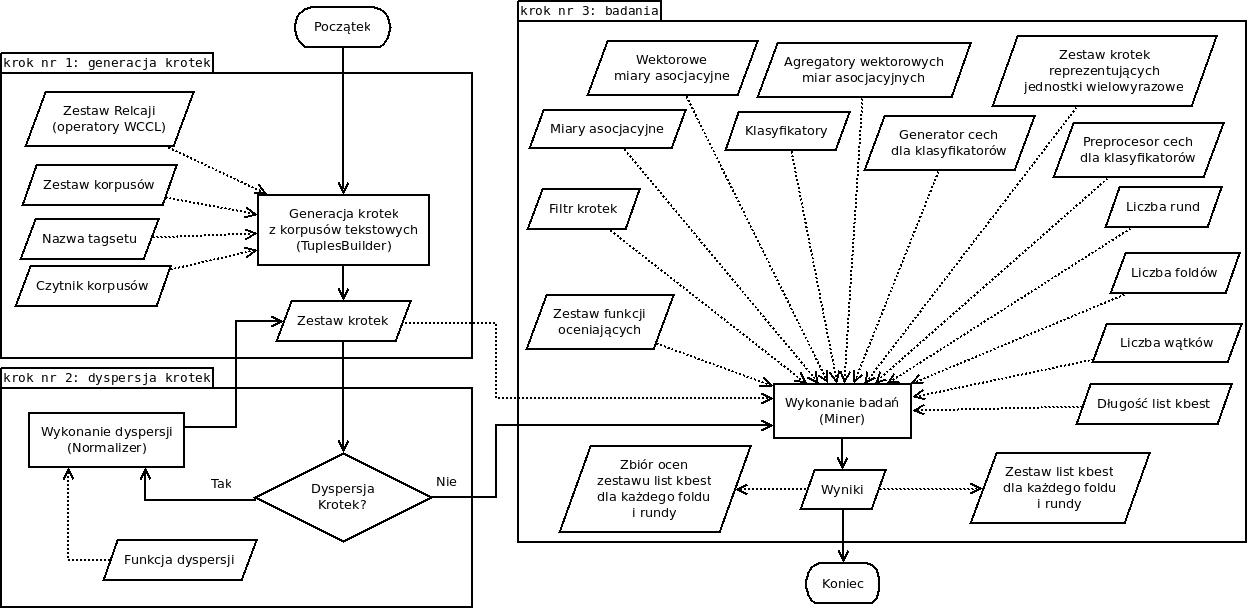
\includegraphics[width=\textwidth]{charts/user_processing_scheme_research.jpg}
\caption [Przykładowy schemat procesu badania jakości rankerów]{Schemat jednego z typowych procesów użytkowania oprogramowania \emph{MWeXtractor} -- badania jakości generowanych przez rankery kolokacji.}
\label{user_processing_scheme_research}
\end{figure}

\par
\noindent\textbf{Krok numer 1: generacja krotek}
\par
Najpierw należy przygotować listę korpusów, z których mają zostać wydobyte dane do przeprowadzenia badań nad metodami ekstrakcji wyrażeń wielowyrazowych.
Należy podać typ czytnika korpusów oraz tagset jakim dane tekstowe zostały opisane.
Następnie zdefiniować zestaw relacji -- operatorów zapisanych w języku \emph{WCCL}, które specyfikują jakich kandydatów na wyrażenia wielowyrazowe należy wyszukiwać w badanych korpusach tekstowych.
Dzięki nim można ograniczyć zestaw kandydatów, nad którymi chce się prowadzić badania.
Jeśli użytkownik jest zainteresowany wszystkimi możliwymi do utworzenia n-gramami może przykładowo wykorzystać do tego celu operator \emph{WCCL} generujący wszystkie możliwe kombinacje n-elementowe.
Zaznaczyć trzeba, że wydobywani kandydaci na kolokacje nie muszą posiadać cechy ciągłości, ich szyk może być zmienny, a wszystko zależy od tego jak zostaną przygotowane relacje.
Tak przygotowany zestaw danych i parametrów należy następnie podać jako argumenty dla programu \emph{TuplesBuilder}, który na ich podstawie przygotuje skład krotek -- podstawową strukturę danych dla oprogramowania \emph{MWeXtractor} składującą krotki.

\par
\noindent\textbf{Krok numer 2: dyspersja krotek}
\par
Drugi krok tego schematu przetwarzania jest opcjonalny i dotyczy modyfikacji informacji o zebranych krotkach -- ich częstości będących kluczowym elementem związanym z późniejszą oceną kandydatów na kolokacje.
Do tego celu wykorzystana może zostać jedna z funkcji dyspersji zaimplementowana w tym celu.
Funkcje te zostaną opisane w dalszej części pracy.
Zależnie od wybranej metody dyspersji pod uwagę brane są różne statystyki związane z krotkami, przykładowo będą to częstości danych krotek, liczba krotek w danym korpusie czy informacja o tym, w ilu korpusach dana krotka została odnaleziona.
Mówiąc inaczej, miara dyspersji ma za zadanie zmienić rozkład częstości krotek w składzie\footnote{Skład krotek to podstawowa struktura do przechowywania danych statystycznych wydobytych z korpusów tekstowych, przechowuje między innymi rodzaje i częstości kandydatów na kolokacje. Jej dokładniejszy opis został zamieszczony w dalszej części niniejszego rozdziału, aby nie wprowadzać szczegółów mogących utrudnić zrozumienie ogólnej koncepcji działania systemu.} promując instancje ciekawe -- mniej typowe.
\par
Jedna z zaimplementowanych funkcji dyspersji\footnote{Funkcje dyspersji zostaną opisane w dalszej części niniejszego rozdziału.} -- \emph{Lynes D3} \cite{dispersions}, bazuje na mierze $ Chi^{2} $, a tym samym potrzebne są jej pewne dane statystyczne.
Jeśli ta miara ma zostać wykorzystana do dyspersji krotek, to trzeba jej owe dane statystyczne przygotować.
Sposób generacji tych informacji został opisany w trzecim kroku kolejnego z przykładowych schematów przetwarzania.
Zaznaczyć jednak trzeba, że miara \emph{Lynes D3} to wyjątek.

\par
\noindent\textbf{Krok numer 3: badania}
\par
Niniejszy krok jest krokiem finalnym ścieżki przetwarzania.
Polega on na wykonaniu r-rundowej, f-foldowej walidacji krzyżowej dla danego zbioru danych, z wykorzystaniem określonych miar asocjacyjnych i klasyfikatorów.
Oprogramowanie przeznaczone do tego celu zostało nazwane \emph{Miner}.
Wyniki wygenerowane przez ten program zostają poddane ocenie przez użytkownika narzędzi \emph{MWeXtractor}. 
Do łączenia dużych zestawów wyników przygotowany został skrypt w języku \emph{Python} uśredniający wyniki dla wszystkich foldów z każdej z rund, dla poszczególnych funkcji rankingowych z osobna.
Pozwala to na szybkie wygenerowanie zbiorczych wyników i na utworzenie wykresów prezentujących jakości rezultatów zastosowanych metod wydobycia według określonych miar.
\par
Parametry programu \emph{Miner} zostały wymienione i opisane w tabeli \ref{miner_parameters}.

\begin{table}[h!]
\centering
\begin{tabular}{l | l | p{0.6\linewidth}}
	\toprule 
	\textbf{Nazwa} & \textbf{Typ} & \textbf{Opis} \\
	\midrule 
	Skład krotek & nazwa folderu & ścieżka do folderu ze składem krotek \\ 
	\hline
	Wyjście programu & nazwa folderu & ścieżka do folderu, w którym zostaną zamieszczone wyniki\\ 
	\hline
	Miary asocjacji & ciągi tekstowe & parametr wielokrotny, tekst reprezentujący funkcje asocjacyjną, którą program ma wykorzystać\\ 
	\hline
	Miary wektorowe & ciągi tekstowe & parametr wielokrotny, tekst reprezentujący wektorową miarę asocjacyjną, którą program ma wykorzystać\\ 
	\hline
	Agregatory & ciągi tekstowe & parametr wielokrotny, tekst reprezentujący funkcję agregującą wyniki miar wektorowych, po jednej funkcji dla każdej z nich\\
	\hline
	Klasyfikatory & ciągi tekstowe & parametr wielokrotny, tekst reprezentujący klasyfikator, który program ma wykorzystać\\ 
	\hline
	Generator cech & ciąg tekstowy & wektorowa miara asocjacyjna, która zostanie wykorzystana jako generator cech dla klasyfikatorów\\ 
	\hline
	Preprocesor cech & ciąg tekstowy & parametr opcjonalny, tekst reprezentujący funkcję, która ma zostać wykorzystana do normalizacji cech\\ 
	\hline
	Zestaw JW & nazwa pliku & plik zawierający w każdej linii ciąg wyrazów oddzielonych spacjami, reprezentujący wyrażenie wielowyrazowe\\ 
	\hline
	Funkcje oceny & ciągi tekstowe & parametr wielokrotny, tekst reprezentujący funkcję oceny, którą program ma wykorzystać\\ 
	\hline
	Filtr krotek & ciąg tekstowy & tekst reprezentujący filtr, który program ma wykorzystać do wyznaczenia zestawu krotek, z których ma korzystać i, dla których wygenerować dane\\ 
	\hline
	Liczba wątków & liczba całkowita & maksymalna liczba wątków do wykorzystania przez program\\ 
	\hline
	Liczba rund & liczba całkowita & liczba rund walidacji krzyżowej\\ 
	\hline
	Liczba foldów & liczba całkowita & liczba foldów dla każdej walidacji krzyżowej\\
	\bottomrule
\end{tabular}
\caption[Parametry programu \emph{Miner}]{Tabela zawiera nazwy, typy oraz opisy parametrów wykorzystywanych przez program \emph{Miner}}
\label{miner_parameters}
\end{table}

\par
Wspomniany zbiór wyników jest obszerny, podzielony na pliki, których są dwa rodzaje -- pliki z listami k-najlepszych kandydatów na wyrażenia wielowyrazowe, oraz pliki z ocenami tych list.
Liczba wygenerowanych plików rankingowych jest równa \( ((A + V + C) * R * F) \), gdzie \emph{A}, \emph{V} oraz \emph{C} oznaczają kolejno liczbę wykorzystanych funkcji asocjacyjnych, wektorowych miar asocjacyjnych oraz klasyfikatorów, natomiast \emph{R} i \emph{F} to kolejno liczba rund i foldów walidacji krzyżowej.
Dodatkowo dla każdego pliku z rankingiem wygenerowanych zostaje \emph{Q} plików oceny tego rankingu, gdzie \emph{Q} jest liczbą wykorzystanych funkcji oceny list k-najlepszych.
Wzorzec nazwy pliku z rankingiem jest generowany w sposób następujący: \emph{kbest.nr\_rankera.nr\_rundy.nr\_foldu.csv}, natomiast wzorzec dla plików z wynikami funkcji oceny list k-najlepszych to: \emph{kbest.nr\_rankera.nr\_rundy.nr\_foldu.nr\_funkcji\_oceny.csv}.
Numer rankera\footnote{Ranker to pojęcie wprowadzone przez autora pracy na ogólne określenie metod i algorytmów generujących rankingi pewnych bytów. W przypadku niniejszej pracy i tematyki tutaj poruszanej rankerami są funkcje asocjacyjne, wektorowe miary asocjacyjne oraz klasyfikatory, a zadaniem każdego z nich jest wygenerowanie rankingu kandydatów na kolokacje.} jest z przedziału:
\begin{enumerate}
  \item \texttt{[0     : A         - 1]} -- dla funkcji asocjacyjnych;
  \item \texttt{[A     : A + V     - 1]} -- dla wektorowych miar asocjacyjnych;
  \item \texttt{[A + V : A + V + C - 1]} -- dla klasyfikatorów.
\end{enumerate}

Ze względu na dużą liczbę plików wynikowych zaimplementowany został skrypt wspomniany wcześniej, łączący wyniki poprzez uśrednienie wyników dla każdego foldu z każdej rundy dla poszczególnych funkcji rankingujących z osobna.
Skrypt ten generuje pojedynczy plik z jedną kolumną dla każdego rankera.
Skrypt nazwany został \emph{cv\_quality\_merger.py}, został napisany w języku \emph{Python} i jest częścią pakietu \emph{MWeXtractor}.


\subsection{Schemat procesu ekstrakcji wyrażeń wielowyrazowych}
Schemat \ref{user_processing_scheme_extraction} prezentuje drugą z dwóch typowych ścieżek przetwarzania, odpowiedzialną za ekstrakcje wyrażeń wielowyrazowych bez wykonywania badań.

\begin{figure}[h!]
\centering
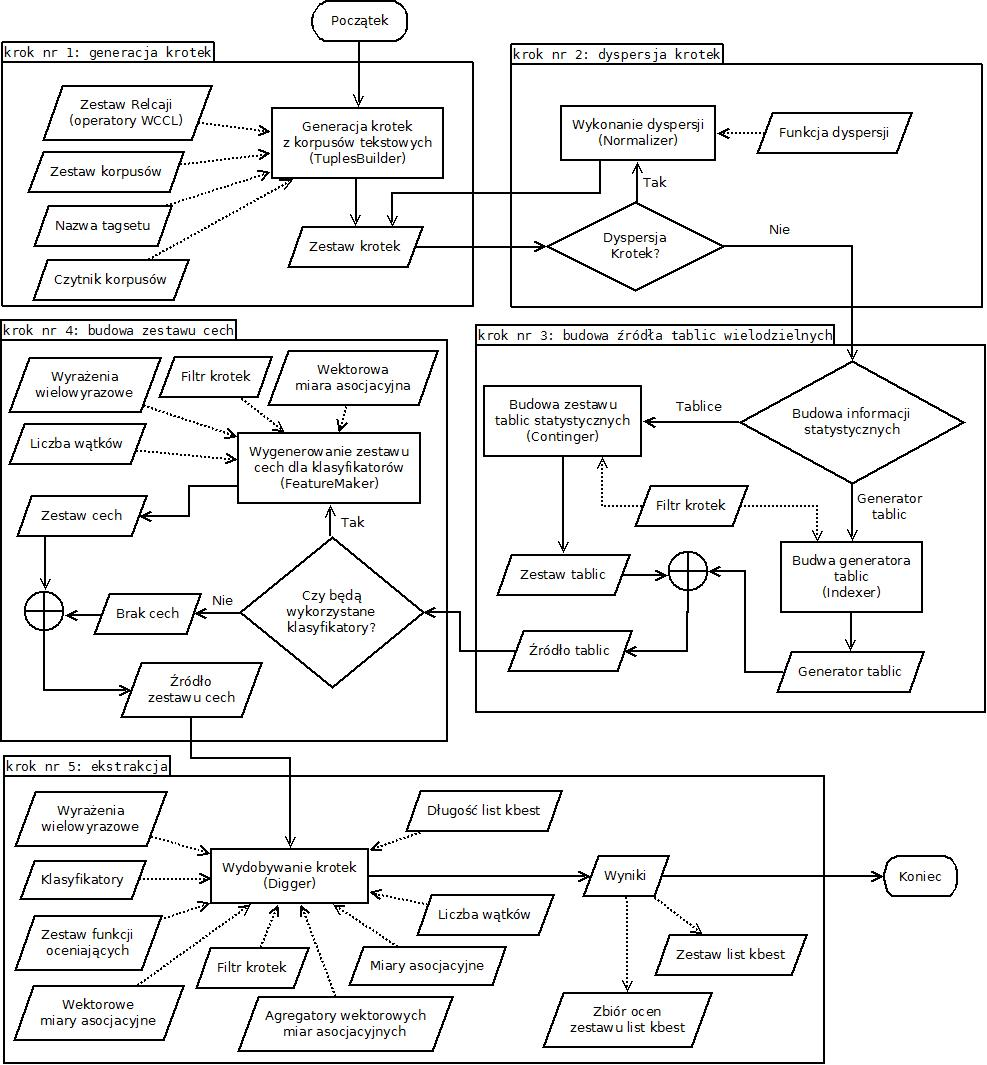
\includegraphics[width=\textwidth]{charts/user_processing_scheme_extraction.jpg}
\caption [Przykładowy schemat procesu wydobywania wyrażeń wielowyrazowych]{Schemat prezentujący jeden z typowych procesów wydobywania wyrażeń wielowyrazowych za pomocą oprogramowania \emph{MWeXtractor}}
\label{user_processing_scheme_extraction}
\end{figure}

\par
\noindent\textbf{Kroki numer 1 i 2}
\par
Oba krotki są takie same jak w przypadku poprzedniego przykładowego schematu przetwarzania -- badania miar asocjacyjnych i klasyfikatorów \footnote{por. rozdz. 4.6.2.}.

\par
\noindent\textbf{Krok numer 3: budowa źródła tablic wielodzielnych}
\par
Wszystkie zaimplementowane miary i klasyfikatory korzystają z informacji zawartych w tablicach wielodzielnych dla krotek. 
Miary korzystają z tych informacji bezpośrednio do obliczania wartości dla kolokacji, a w przypadku klasyfikatorów miary te wykorzystywane są do generowania cech instancji.
Wyjątkiem są miary oparte na szyku, ponieważ nie korzystają z takich informacji.
Krok trzeci polega na utworzeniu jednego z dwóch dostępnych źródeł tablic -- ich generatora lub składu. 
Programy przygotowane do wykonania tego zadania to odpowiednio \emph{Indexer} oraz \emph{Continger}.
Zazwyczaj generator tablic zajmuje znacznie mniej pamięci operacyjnej -- kilkakrotnie mniej niż tablice wielodzielne, ale odwołanie się do tablic jest znacznie wolniejsze niż w przypadku składu tablic, ponieważ generator tworzy je na bieżąco, a skład przechowuje już gotowe tablice.
Zestaw krotek, na podstawie których źródło tablic ma zostać wygenerowane można ograniczyć za pomocą filtrów.
Zabieg taki pozwala na używanie określonego składu krotek do różnych celów, bez konieczności wydobywania kandydatów z korpusów wielokrotnie.
Dodatkowo umożliwia to zbudowanie informacji statystycznych na podstawie innego zestawu krotek niż ten, z którego wyrażenia wielowyrazowe mają być wydobywane.
Jako praktyczny przykład takiego zadania można podać ten, w którym informacja statystyczna budowana jest na podstawie krotek zebranych za pomocą relacji okna, a wydobywanie wyrażeń wielowyrazowych jedynie na podstawie innych relacji, przykładowo o określonych wzorcach strukturalnych.

\par
\noindent\textbf{Krok numer 4: budowanie zestawu cech}
\par
Niniejszy krok jest opcjonalny i może zostać pominięty, jeśli użytkownik nie ma zamiaru korzystać z klasyfikatorów.
Jeżeli jednak użytkownik będzie chciał skorzystać z klasyfikatorów lub wygenerować zestaw cech, z których będzie można korzystać w oprogramowaniu \emph{WEKA}, może do tego celu użyć programu o nazwie \emph{FeatureMaker}.
Zadaniem tego modułu jest wygenerowanie cech dla kandydatów na kolokacje, spośród których mają być w przyszłości wydobyte wyrażenia wielowyrazowe.
Do wykonania tego zadania generator cech wykorzystuje miary asocjacyjne, których wyniki traktowane są jako cechy.
Dopuszczalne jest także wykorzystanie uprzednio wyuczonych klasyfikatorów, przykładowo sieci neuronowych, do generowania cech opisujących kandydatów.
Zestaw kandydatów można ograniczyć za pomocą filtru jeśli nie ma potrzeby wyznaczenia cech dla wszystkich krotek.
\par
Aktualnie jedynym wspieranym formatem pliku wykorzystywanym do zapisu zestawu cech w pamięci nieulotnej, jest \emph{ARFF}.
\par
Tabela \ref{feature_maker_parameters} zawiera opisy parametrów programu \emph{FeatureMaker}.

\begin{table}[h!]
\centering
\begin{tabular}{l | l | p{0.6\linewidth}}
	\toprule 
	\textbf{Nazwa} & \textbf{Typ} & \textbf{Opis} \\
	\midrule 
	Skład krotek & nazwa folderu & ścieżka do folderu ze składem krotek \\ 
	\hline
	Wyjście programu & nazwa pliku & ścieżka do pliku, w którym zostaną zapisane wyniki\\ 
	\hline
	Zestaw JW & nazwa pliku & plik zawierający w każdej linii ciąg wyrazów oddzielonych spacjami, reprezentujący wyrażenie wielowyrazowe, wykorzystany w przypisywaniu klas krotkom\\ 
	\hline
	Generator cech & ciągi tekstowe & tekst reprezentujący wektorową miarę asocjacyjną, którą program ma wykorzystać do generowania cech dla krotek\\ 
	\hline
	Filtr krotek & ciąg tekstowy & tekst reprezentujący filtr, który program ma wykorzystać do wyznaczenia zestawu krotek, dla których wygenerować cechy\\ 
	\hline
	Liczba wątków & liczba całkowita & maksymalna liczba wątków do wykorzystania przez program\\ 
	\bottomrule
\end{tabular}
\caption[Parametry programu \emph{FeatureMaker}]{Tabela zawierająca nazwy, typy oraz opisy parametrów wykorzystywanych przez program \emph{FeatureMaker}}
\label{feature_maker_parameters}
\end{table}

\par
\noindent\textbf{Krok numer 5: ekstrakcja}
\par % TODO: Digger modifications: classifiers + features
Ostatnim krokiem tej ścieżki przetwarzania jest wykorzystanie wcześniej utworzonych danych do ekstrakcji wyrażeń wielowyrazowych z korpusów tekstowych.
Zadanie to może zostać wykonane za pomocą programu \emph{Digger}.
Zestaw parametrów programu jest zbliżony do tych dla narzędzia \emph{Miner}.
W tabeli \ref{digger_parameters} opisane zostały argumenty dla oprogramowania \emph{Digger}.

\begin{table}[h!]
\centering
\begin{tabular}{l | l | p{0.6\linewidth}}
	\toprule 
	\textbf{Nazwa} & \textbf{Typ} & \textbf{Opis} \\
	\midrule 
	Skład krotek & nazwa folderu & ścieżka do folderu ze składem krotek \\ 
	\hline
	Źródło tablic & nazwa pliku & ścieżka do pliku ze składem lub generatorem krotek\\
	\hline
	Wyjście programu & nazwa folderu & ścieżka do folderu, w którym zostaną zamieszczone wyniki\\ 
	\hline
	Miary asocjacji & ciągi tekstowe & parametr wielokrotny, tekst reprezentujący funkcje asocjacyjną, którą program ma wykorzystać\\ 
	\hline
	Miary wektorowe & ciągi tekstowe & parametr wielokrotny, tekst reprezentujący wektorową miarę asocjacyjną, którą program ma wykorzystać\\ 
	\hline
	Agregatory & ciągi tekstowe & parametr wielokrotny, tekst reprezentujący funkcję agregującą wyniki miar wektorowych, po jednej funkcji dla każdej z nich\\
	\hline
	Klasyfikatory & ciągi tekstowe & parametr wielokrotny, tekst reprezentujący klasyfikator, który program ma wykorzystać\\ 
	\hline
	Źródło cech & nazwa pliku & Źródło zestawu cech dla krotek\\ 
	\hline 
	Zestaw JW & nazwa pliku & plik zawierający w każdej linii ciąg wyrazów oddzielonych spacjami, reprezentujący wyrażenie wielowyrazowe\\ 
	\hline
	Funkcje oceny & ciągi tekstowe & parametr wielokrotny, tekst reprezentujący funkcję oceny, którą program ma wykorzystać\\ 
	\hline
	Filtr krotek & ciąg tekstowy & tekst reprezentujący filtr, który program ma wykorzystać do wyznaczenia zestawu krotek, z których ma korzystać i, dla których wygenerować dane\\ 
	\hline
	Liczba wątków & liczba całkowita & maksymalna liczba wątków do wykorzystania przez program\\ 
	\bottomrule
\end{tabular}
\caption[Parametry programu \emph{Digger}]{Tabela zawierająca nazwy, typy oraz opisy parametrów wykorzystywanych przez program \emph{Digger}}
\label{digger_parameters}
\end{table}

Zestaw generowanych wyników jest podobny do tego, który generuje narzędzie \emph{Miner}, ale jest mniejszy, ponieważ nie ma podziału na rundy i foldy ze względu na brak walidacji krzyżowej.
Wzorce nazw dla plików k-najlepszych krotek i plików z ocenami prezentują się teraz następująco: \emph{kbest.nr\_rankera.csv} oraz \emph{quality.nr\_rankera.nr\_funkcji\_oceny.csv}.
Zasada generowania numeru rankera jest taka sama jak w przypadku programu \emph{Miner}.


\subsection{Funkcjonalności dodatkowe}
Pakiet narzędzi \emph{MWeXtractor} posiada też dodatkowe funkcjonalności, z których część została opisana w tym rozdziale.

\par
\noindent\textbf{Program \textit{Cover}}
\par
Program nazwany \emph{Cover} służy do weryfikacji relacji oraz badania przecięcia zbioru wydobytych krotek pomiędzy relacjami -- sprawdzenia, jak wiele z nich zostało przyporządkowanych do więcej niż jednej relacji.
Praktyczne wykorzystanie tego oprogramowania to sprawdzenie pokrycia wzajemnego operatorów \emph{WCCL} zastosowanych do wydobywania krotek z tekstów.
Wynikiem jego działania jest macierz kwadratowa o wymiarze równym liczbie relacji wykorzystanych w procesie tworzenia \emph{składu krotek}, gdzie każdy z wierszy i każda z kolumn mają przypisaną do siebie określoną nazwę operatora \emph{WCCL}.
Liczby całkowite zapisane na przecięciu wierszy z kolumnami informują, ile różnych krotek zostało przypisanych zarówno do relacji będącej etykietą wiersza, jak i kolumny.
Interpretacją liczby na przecięciu wiersza i kolumny -- diagonali, odpowiadającym tej samej relacji jest informacja o tym, ile krotek zostało zakwalifikowanych do tej relacji.
Jeśli w danym wierszu lub kolumnie, poza polem na diagonali macierzy, wystąpi więcej niż jedna wartość większa od zera  oznacza to, że relacje są nierozłączne -- część krotek przyporządkowano do więcej niż jednej relacji.
Należy jednak pamiętać, że narzędzie to nie jest wyrocznią, ponieważ jeśli dla danego zbioru danych okaże się, że relacje są rozłączne, nie oznacza to, że dla innego zbioru, większego czy lepiej oddającego rzeczywistość, sytuacja się powtórzy.
Zbudowana w ten sposób macierz jest symetryczna.
\par
Opisywany tutaj program \emph{Cover} ma także drugie zastosowanie wspomniane we wcześniejszej części tego fragmentu pracy -- badanie przecięcia zbioru krotek ze składu i zestawu zadanego parametrem programu.
Na podstawie zadanego pliku z ciągami wyrazów program bada ile z nich, oraz które konkretnie ciągi zostały odnalezione w \emph{składzie krotek}.
Funkcjonalność ta może posłużyć przykładowo do wyznaczania zbioru krotek pozytywnych, czyli wyrażeń wielowyrazowych, które zostały w tym tekście odnalezione podczas wydobywania kandydatów na kolokacje.
Dodatkowo zakres poszukiwań wśród krotek w składzie można zawęzić za pomocą filtru.
Zabieg taki pozwala na lepsze poznanie zbioru danych.

\par
\noindent\textbf{Wydobywanie form napotkanych}
\par
Program \emph{Digger} umożliwia dodatkowo wydobycie form napotkanych dla krotek z wygenerowanych list k-najlepszych kandydatów na kolokacje.
Jeśli użytkownik jest zainteresowany ekstrakcją form napotkanych to powinien podać cztery dodatkowe parametry dla tego programu, które zostały opisane w tabeli \ref{digger_parameters_orths}.

\begin{table}[h!]
\centering
\begin{tabular}{l | l | p{0.5\linewidth}}
	\toprule 
	\textbf{Nazwa} & \textbf{Typ} & \textbf{Opis} \\
	\midrule 
	Zestaw korpusów & nazwa pliku & ścieżka do pliku zawierającego listę ścieżek do korpusów, po jednej ścieżce w każdej linii pliku \\ 
	\hline
	Operatory WCCL & nazwa pliku & ścieżka do pliku z operatorami języka \emph{WCCL}, które były użyte przy wydobywaniu kandydatów na kolokacje w kroku numer jeden\\ 
	\hline
	Tagset & ciąg znaków & nazwa wykorzystanego tagsetu w korpusach \\
	\hline
	Czytnik & ciąg znaków & nazwa czytnika korpusów\\
	\bottomrule
\end{tabular}
\caption[Parametery dodatkowe programu \emph{Digger}]{Tabela zawierająca nazwy, typy oraz opisy parametrów dodatkowych wykorzystywanych przez program \emph{Digger}.}
\label{digger_parameters_orths}
\end{table}

Wyekstrahowany zestaw form napotkanych dla krotek zostanie zapisany w pojedynczym pliku w formacie \emph{CSV}.
Format pliku jest następujący: najpierw zapisana zostaje reprezentacja krotki z jednej z list k-najlepszych, a część kolejnych linii rozpoczyna się tabulacją i zawiera ciąg wyrazów napotkanych dla tej krotki wraz z jego częstością.
Następnie zapis taki powtarza się dla wszystkich wydobytych krotek, jeśli jest ich więcej, ale bez powtórzeń, jeśli krotki wystąpiły na różnych listach k-najlepszych.
Dodatkowo napisany został skrypt łączący listy k-najlepszych z zestawem wydobytych dla nich form napotkanych i tworzący nowe listy k-najlepszych z zachowaniem przy tym kolejności rankingu.
Skrypt przypisuje również do każdej pozycji zestaw form napotkanych tej krotki wraz z ich częstościami.
Kolejność form napotkanych po łączeniu będzie posortowana malejąco według ich częstości.
Skrypt ten, napisany w języku \emph{Python}, został nazwany \emph{kbest\_orth\_merger.py} i jest częścią pakietu \emph{MWeXtractor}.


\subsection{Format składowania krotek zebranych z korpusów}
Jako format przechowywania danych wykorzystano krotki o różnych długościach\footnote{Długość krotki rozumiana jest jako liczba jej elementów składowych, przykładowo wyrazów.} co umożliwia składowanie informacji o wyrażeniach wielowyrazowych dowolnej długości w intuicyjny sposób.
Krotki są dość powszechnym, elastycznym i prostym formatem stosowanym do przechowywania danych, a dodatkowo zapisywane są w postaci tekstu czytelnego dla człowieka, co czyni format przejrzystym, łatwym do ewentualnej edycji i ułatwia analizę zapisanych informacji.

\par
Krotka reprezentująca wyrażenie wielowyrazowe zawiera w sobie słowa w ustalonej kolejności wraz z ich częściami mowy, które wchodzą w skład tego wyrażenia.
Każda z krotek zawiera także informację, w jakiej relacji wystąpiły zawarte w tej krotce wyrazy.
Relacja jest jednym z operatorów \emph{WCCL} wykorzystanym w procesie tworzenia krotek na podstawie korpusów --- proces ten został opisany w dalszej części tej sekcji.
Jeśli dane zestawienie wyrazów w tekście spełnia wymagania dla kilku różnych wyrażeń języka ograniczeń \emph{WCCL}, to dla każdego z nich powstanie osobna krotka zawierająca te same elementy, ale różniąca się relacją.
Dodatkowo w krotce zawarte są metadane o niej, takie jak jej częstość\footnote{Częstość krotki określa liczbę wystąpień konkretnego zestawienia słów w danej relacji.} w przetworzonych korpusach danych.
Relacja nie jest uwzględniana w rozmiarze krotki.
Format składowania krotek w pliku tekstowym wraz z przykładem został zamieszczony w tabeli \ref{tuple_format}.

\begin{table}[h!]
\centering
\begin{tabular}{l l l l l l}
\toprule
	\textbf{nazwa relacji} & 
		\textbf{arność relacji} & 
		\textbf{częstość krotki} & 
		\textbf{cz.m.:s1} & 
		\textbf{cz.m.:s2} & 
		\ldots \\
	\midrule
	AdjSubst & 2 & 17 & adj:nowy & subst:but & \\
\bottomrule
\end{tabular}
\caption[Format składowania krotek w pliku tekstowym]{Format składowania krotek w pliku tekstowym wraz z przykładem. Elementy (ciągi znakowe) składowane w pliku tekstowym oddzielone są od siebie tabulatorami. Arność relacji jest tożsama z rozmiarem krotki. Skrótowiec \emph{cz.m:sN} pochodzi od: część mowy, dwukropek, \emph{N}-te słowo krotki.}
\label{tuple_format}
\end{table}
\par
Istotnym elementem przetwarzania tak dużych zbiorów danych jest wydajny sposób składowania ich w pamięci operacyjnej maszyny przetwarzającej.
Do tego celu opracowana, zaimplementowana i wykorzystana została struktura, starająca się minimalizować zużycie pamięci przy zachowaniu szybkiego dostępu do danych poprzez wykorzystanie implementacji zbiorów opartych o drzewa czerwono-czarne i funkcje skrótu\footnote{Popularna nazwa anglojęzyczna to \emph{hash function} - funkcja haszująca.}.
Struktura składa się z pięciu modułów odpowiedzialnych za przechowywanie innych informacji.

\par
Moduł numer jeden zawiera w sobie informacje o wykorzystanych korpusach.
Zapisana jest nazwa korpusu, ścieżka do pliku z tym korpusem, a także częstości słów w każdym z korpusów z osobna oraz suma wystąpień tych wyrazów.

\par
Drugi z modułów zawiera w sobie podzbiór części mowy występujących w tagsecie wykorzystanym do opisu morfosyntaktycznego korpusów danych użytych do ekstrakcji kandydatów na wyrażenia wielowyrazowe.
Podzbiór ten zawiera tylko te części mowy, które wystąpiły przynajmniej raz w przetwarzanych tekstach, ale nic nie stoi na przeszkodzie, by dodać także części mowy niewchodzące w skład wykorzystanego tagsetu.

\par
Trzeci moduł wykorzystuje informacje z modułu związanego z częściami mowy wyrazów. 
Jego zadaniem jest składowanie wszystkich słów wraz z przyporządkowanymi im częściami mowy oraz częstością tych właśnie wyrazów wygenerowaną na podstawie korpusów tekstowych.
Moduł musi przechowywać wszystkie słowa, które będą składowymi krotek, ale może przechowywać także wyrazy nadmiarowe.

\par
Moduł numer cztery składuje dane o relacjach, jakie zostały użyte do tworzenia krotek na podstawie korpusów tekstowych.
Przechowywane są w nim informacje takie jak nazwy relacji, arności określające długość generowanych krotek oraz liczba krotek, które zostały utworzone z wykorzystaniem tej właśnie relacji.
Relacje, które nie wykreowały żadnego kandydata na kolokacje, także są w tym składzie uwzględnione wraz z informacjami o nich.
Ważną informacją jest także fakt, że w tej strukturze nie są przechowywane ciała wyrażeń \emph{WCCL} definiujących daną relację.

\par
Piąty z modułów jest odpowiedzialny za składowanie krotek oraz metadanych je opisujących.
Struktura składowania tych danych może być postrzegana jako \emph{N-hipermacierz} \cite[rozdział 15]{hypermat}, której liczba wymiarów \emph{N} jest równa długości najdłuższej z krotek, powiększonej o jeden, formalnie:
$$ N = 1 + maks(rozmiar(k) \: \forall k \in K : K = \{zestaw \: wszystkich \: krotek\}) $$

Każdy wymiar odpowiada jednemu ze słów krotki lub jej relacji.
Pierwsze \emph{K} wymiarów odpowiada kolejno wyrazom kolokacji wraz z ich częściami mowy, a wymiar \emph{K + 1} jest interpretowany jako opisujący relację tej krotki.
Prostymi wnioskami są \( (K + 1) <= N \) oraz to, że nie wszystkie wymiary w macierzy dla danej krotki są zawsze wykorzystane.
Przykładowo rozważmy skład zawierający w sobie tylko dwie poniższe krotki:

\begin{table}[h!]
\centering
\begin{tabular}{c c c c c c}
\toprule
\textbf{relacja} & \textbf{arność} & \textbf{cz.m:s1} & \textbf{cz.m:s2} & \textbf{cz.m:s3} & \textbf{częstości...} \\ 
\midrule
  AdjSubstAdj & 3 & adj:czerwony & subst:samochód & adj:sportowy & ... \\
  AdjSubst & 2 & adj:czerwony & subst:kartka & [brak] & ... \\
\bottomrule
\end{tabular}
\end{table}

Dla podanego zestawu krotek wymiar hipermacierzy będzie równy cztery - trzy wyrazy najdłuższej z krotek plus jeden.
Pierwszy wymiar tej hipermacierzy dla obu krotek opisuje pierwszą składową krotki - dla obu z nich będzie to \emph{adj:czerwony}.
Drugi wymiar zawiera informacje o drugiej składowej kandydatów na kolokacje i są to odpowiednio słowa \emph{subst:samochód} oraz \emph{subst:kartka}.
Trzeci wymiar w przypadku pierwszej krotki odpowiada jej trzeciej składowej, a w przypadku krotki numer dwa - jej relacji.
Ostatni z wymiarów, czwarty, jest zdefiniowany tylko dla dłuższej z obu krotek i odnosi się do jej relacji.
\emph{Hipermacierz} krotek jest indeksowana słowami wraz z ich częściami mowy i opcjonalnie za pomocą relacji.
Podczas odnoszenia się do tej macierzy nie jest wymagane podanie wszystkich składowych indeksu\footnote{Pojęcie indeksu odnosi się do struktury wykorzystywanej do odwoływania się do danych w \emph{hipermacierzy} krotek.} - wszystkich słów i relacji, ale wymagane jest określanie wartości po kolei - nie mogą powstać dziury pomiędzy zdefiniowanymi wartościami dla wymiarów, zachowana musi zostać ciągłość w procesie tworzenia indeksu.
Zapis formalny ciągłości indeksu:

\begin{center}
\( \forall D_{i} : D_{i} \in D = \{wymiary \: hipermacierzy \}, i \geq 1 \: \exists D_{i-1} : wartosc(D_{i-1}) \: \neq \: niezdefiniowany \)
\end{center}

Tabela \ref{hypermatrix_indices} ilustruje przytoczony wcześniej przykład i zawiera instancje poprawnych oraz błędnych (nieciągłych) indeksów dla \emph{4-hipermacierzy} krotek.

\begin{table}[h!]
\centering
\begin{tabular}{c c c c c}
\toprule
\textbf{cz.m:s1} & \textbf{cz.m:s2} & \textbf{cz.m:s3} & \textbf{relacja}  & \textbf{poprawny} \\
\midrule
adj:ładny, 	& subst:samochód, 	& adj:sportowy		& AdjSubstAdj	& tak \\
adj:ładny, 	& subst:samochód, 	& - ,			& -		& tak \\
adj:ładny,	& - ,			& - ,			& -		& tak \\
- ,		& subst:samochód, 	& adj:sportowy 		& -		& nie \\
- ,		& adj:ładny,		& subst:samochód	& AdjSubstAdj	& nie \\
adj:ładny,	& adj:ładny,		& - ,			& AdjSubstAdj	& nie \\
\bottomrule
\end{tabular}
\caption
	[Przykładowe indeksy dla \emph{4-hipermacierzy} krotek]
	{Przykładowe indeksy dla \emph{4-hipermacierzy} krotek. Wszystkie przykłady niepoprawnych indeksów złamały tę samą zasadę dotyczącą ciągłości indeksu - nie można definiować wartości dla wymiaru \emph{D} jeśli nie została ona zdefiniowana dla \emph{D - 1} (\emph{D = 0} jest wyjątkiem).}
\label{hypermatrix_indices}
\end{table}

\par
Niech pojęcie \emph{I-indeks} odnosi się do indeksu \emph{I}-elementowego, czyli struktury ze zdefiniowanymi \emph{I} elementami odpowiedzialnymi za indeksowanie danych w \emph{hipermacierzy} krotek.
Efektem wykorzystania \emph{I-indeksu} do odwołania się do danych w \emph{N-hipermacierzy} krotek jest \emph{K-hipermacierz} danych\footnote{W przypadku indeksu o rozmiarze zero tej samej \emph{hipermacierzy}.}, gdzie spełniona jest nierówność \( K <= N \), a liczba wymiarów \emph{K} jest zależna od \emph{N} oraz \emph{I} i równa:

\begin{center}
\( K = N - I \)
\end{center}

Wartość \emph{K = 0} jest całkowicie poprawna i oznacza skalar, konkretną krotkę, \emph{K = 1} oznacza wektor, dla \emph{K = 2} jest macierzą dwuwymiarową, \emph{K = 3} to \emph{3-hipermacierz} i tak dalej.
Dla wyjaśnienia i lepszego zrozumienia indeksowania rozważmy poniższą \emph{hipermacierz} z przyporządkowaniem wierszom, kolumnom itd. liczb zamiast słów i relacji.
\begin{center}
\[
M = 
\left[
\begin{array}{c c c | c c c}
1 	& 2 	& 3 	& 4 	& 5 	& 6 	\\
11 	& 12 	& 13 	& 14 	& 15 	& 16 	\\
21 	& 22 	& 23 	& 24 	& 25 	& 26 	\\
31 	& 32 	& 33 	& 34 	& 35	& 36 	\\
\end{array}
\right]
\]
\end{center}

Powyższy zapis symbolizuje \emph{3-hipermacierz} liczb naturalnych o wymiarach \emph{4 x 3 x 2} - cztery wiersze, trzy kolumny oraz dwie warstwy, indeksowane od zera. 
Liczby 1, 11, 21, 31 oraz 4, 14, 24, 34 są etykietami wierszy, 1, 2, 3 oraz 4, 5, 6 etykietami kolumn, a liczby 1 oraz 4 są także etykietami warstw tej macierzy.
Część po lewej stronie pionowej linii odzwierciedla pierwszą warstwę \emph{hipermacierzy}, a po prawej drugą.
Utworzenie i wykorzystanie 1-indeksu postaci \( [4, -, -] \) zwróci zredukowaną do dwóch wymiarów macierz będącą po prostu drugą warstwą \emph{3-hipermacierzy} wyjściowej, postaci:

\[
M[4] = 
\left[
\begin{array}{c c c}
4 	& 5 	& 6 	\\
14 	& 15 	& 16 	\\
24 	& 25 	& 26 	\\
34 	& 35	& 36 	\\
\end{array}
\right]
\]

Dodanie wartości 5 do 1-indeksu spowoduje tym razem utworzenie 2-indeksu postaci \( [4, 5, -] \), którego wykorzystanie zaowocuje odwołaniem się do konkretnego wektora - kolumny, zawierającego się w macierzy i równego:

\[
M[4, 5] = 
\left[
\begin{array}{c}
5 \\
15 \\
25 \\
35 \\
\end{array}
\right]
\]

Ostatecznie rozwinięcie 2-indeksu o jeszcze jedną wartość, przykładowo 25, i utworzenie 3-indeksu \( [4, 5, 25] \), a następnie odwołanie się za jego pomocą do rozważanej \emph{3-hipermacierzy} liczb spowoduje zwrócenie konkretnej krotki zawierającej kolejne słowa oznaczone numerami 4 i 5 i przyporządkowanej do relacji oznaczonej liczbą 25.
Dodać należy, że kolejność interpretacji wymiarów jest jednak dowolna i nie musi przebiegać w tej kolejności.

\par
Wykorzystanie indeksów dłuższych niż \emph{N} dla \emph{N-hipermacierzy} nie jest też błędem, ale spowoduje niezwrócenie żadnej wartości.
Podanie indeksu niepełnego, tak jak było napisane we wcześniejszej części tego fragmentu pracy, zwróci w ogólności pewną \emph{hipermacierz}, a tym samym zestaw krotek.
Innymi słowy można się odwoływać do konkretnego zestawu krotek spośród całego ich zbioru. 
Każda z krotek zwróconych poprzez wykorzystanie \emph{I}-indeksu będzie miała \emph{I} pierwszych elementów takich jak w indeksie, a reszta będzie dowolnymi elementami.
Także relacja może być konkretna jeśli zostanie podana jako składowa indeksu.
Możliwe jest utworzenie indeksu nie posiadającego zdefiniowanego żadnego z elementów, a jego wykorzystanie zaowocuje zwróceniem pełnej hipermacierzy.


\subsection{Przedstawienie sposobu wydobywania i przechowywania informacji statystycznych wykorzystywanych w obliczeniach}
Przed omówieniem szczegółów dotyczących składowania i pozyskiwania danych wprowadzone zostaną następujące oznaczenia, które będą także wykorzystywane w dalszej części tej pracy.
Oznaczenia zostały zamieszczone na poniższym spisie:

\begin{enumerate}
	\item \( \bar{x} \) - element inny niż \emph{x};
	\item \( n \) - długość krotki;
	\item \( N \) - liczba wszystkich krotek w zbiorze danych;
	\item \( f(x) \) - częstość \emph{x}, wartość zaobserwowana, liczba wystąpień;
	\item \( p(x) \) - prawdopodobieństwo \emph{x};
	\item \( \hat{f}(x) \) - wartość oczekiwana \emph{x};
	\item \( FA(x, y) \) - wartość funkcji asocjacyjnej dla elementów \emph{x} oraz \emph{y}.
\end{enumerate}

\par
Podstawowymi danymi, stosowanymi w procesie wydobywania wyrażeń wielowyrazowych z grona kandydatów, są tablice wielodzielne dla krotek, skonstruowane przy wykorzystaniu częstości kolokacji zebranych z korpusów tekstowych.
Tablica wielodzielna jest terminem stosowanym w niniejszej pracy, rozumianym jako n-wymiarowa tablica, której rozmiar każdego z wymiarów jest równy dwa.
Liczba wymiarów tej tablicy jest równa $ 2^{n} $, a każde jej pole jest numerowane w implementacji od $ 0 $ do $ n - 1 $.
W dalszych częściach pracy dla uproszczenia przyjęta zostanie numeracja od $ 1 $ do $ n $.
Omówiony tutaj zostanie sposób generowania tablicy dla wartości zaobserwowanych z danych, natomiast metoda dla drugiej z tablic zostanie opisana w dalszej części tego rozdziału.
Pierwszy indeks tablicy zawiera informacje o częstości konkretnej krotki, gdzie każdy z elementów jest znany, a kolejne pola tej \emph{hiperkości} zawierają informacje o liczbie wystąpień innych krotek, które mają tylko część składowych takich samych, czyli wyrazy i relację.
Ostatnie pole w tej tablicy informuje o tym, ile jest krotek takich, że wszystkie ich elementy składowe są inne niż te, dla których tablica została utworzona.
Kolejne pola tablicy zawierają informacje o częstościach kolejnych krotek: $ x_{1}, x_{2}, x_{3}, ..., x_{n} $, $ x_{1}, \bar{x}_{2}, x_{3}, ..., x_{n} $, $ \bar{x}_{1}, x_{2}, x_{3}, ..., x_{n}, $, $ \bar{x}_{1}, \bar{x}_{2}, x_{3}, ..., x_{n} $, a pełna tablica zawiera informacje o częstościach dla wszystkich możliwych kombinacji.
Przykładowa tablica dla trójelementowej krotki została zaprezentowana w tabeli \ref{observed_contingency_table}.

\begin{table}[h!]
\centering
\begin{tabular}{c | c}
	\toprule
	Indeks.	& częstość krotki zawierającej elementy									\\
	\midrule
	1. 		& \( x_{1}, 		x_{2}, 			x_{3} \)		\\
	2. 		& \( x_{1}, 		\bar{x}_{2}, 	x_{3} \)		\\
	3. 		& \( \bar{x}_{1}, 	x_{2}, 			x_{3} \)		\\
	4. 		& \( \bar{x}_{1}, 	\bar{x}_{2}, 	x_{3} \)		\\
	5. 		& \( x_{1}, 		x_{2}, 			\bar{x}_{3} \)	\\
	6. 		& \( x_{1}, 		\bar{x}_{2}, 	\bar{x}_{3} \)	\\
	7. 		& \( \bar{x}_{1}, 	x_{2}, 			\bar{x}_{3} \)	\\
	8. 		& \( \bar{x}_{1}, 	\bar{x}_{2}, 	\bar{x}_{3} \)	\\
	\bottomrule
\end{tabular}
\caption[Tablica wielodzielna dla krotki trójelementowej]{Przykładowa tablica wielodzielna, obrazująca informacje o częstościach w niej składowanych.}
\label{observed_contingency_table}
\end{table}

Indeksowanie tablicy dla innej liczby argumentów przebiega analogicznie.
Wzory zamieszczone w dalszej części tego rozdziału mogą wykorzystywać informacje z takiej tablicy poprzez zapis $ t(i) $, co oznacza odwołanie do \emph{i-tego} elementu tablicy utworzonej dla konkretnego kandydata na kolokacje.

\par
Oprogramowanie \emph{MWeXtractor} umożliwia tworzenie omówionych tablic wielodzielnych na dwa sposoby, tak jak wspomniano wcześniej przy okazji opisu schematu przetwarzania.
Jedna z nich to utworzenie gotowego składu tablic wielodzielnych dla każdego kandydata na wyrażenie wielowyrazowe, zaś drugi to przygotowanie generatora, który tworząc odpowiedni indeks będzie w stanie generować tablice wielodzielne dla kolokacji w trakcie działania programu.
Obie przedstawione metody w efekcie generują takie same, tego samego typu wyniki -- tablice wielodzielne.
Bez względu na wykorzystaną metodę tworzenia takich tablic, ich efektem będzie struktura nazywana \emph{Źródłem tablic wielodzielnych}.
Proces tworzenia tablic z wartościami zaobserwowanymi składa się z kilku kroków.
Pierwszym z nich jest wyselekcjonowanie zestawu krotek, które mają zostać wykorzystane do budowy tablic wielodzielnych, za pomocą zaimplementowanego mechanizmu filtrów.
Kolejnym zadaniem jest już właściwy proces budowania tablic.
Polega on na utworzeniu generatora poprzez zbudowanie indeksu, zawierającego informacje o częstościach danych krotek, a także sumy częstości krotek utworzonych poprzez kombinacje elementów składowych tych kolokacji.
Kombinacje te są rozumiane analogicznie jak te, które były przedstawione w opisie tablic wielodzielnych z tym, że zamiast \emph{elementu innego niż} ($ \bar{x} $) stosowany jest zapis mówiący o tym, że element jest dowolny.
Następnie gotowy generator może być już wykorzystany do tworzenia tablic wielodzielnych lub można na jego podstawie wygenerować pełny skład tablic dla konkretnych krotek.
\par
Generowanie tablic z wartościami oczekiwanymi z próby jest procesem szybszym od zbierania danych o wartościach zaobserwowanych, polegającym na obliczeniu iloczynu prawdopodobieństw odpowiadających konkretnym elementom krotki.
Wynik ten jest przemnożony przez liczbę wszystkich krotek o zadanej długości, przykładowo dwuelementowych.
Dane do tych obliczeń pozyskiwane są z tablicy wielodzielnej wartości zaobserwowanych.
Jeśli element krotki jest określony i konkretny, jego oszacowanie prawdopodobieństwa jest równe $ \frac{f(element)}{E} $, gdzie $ E $ jest sumą częstości wszystkich krotek dwuelementowych w generatorze (uwzględnionych w obliczeniach po zastosowaniu filtru).
Natomiast jeśli element krotki jest zanegowany, czyli \emph{inny niż}, to jego prawdopodobieństwo wykorzystane we wzorze jest równe $ 1 - p(element) $.
Dla lepszego zrozumienia tego zagadnienia rozważmy przykład obliczenia wartości oczekiwanej dla krotki 3-elementowej $ (A \bar{B} C) $, gdzie $ E = 10 $, $ A = 1 $, $ B = 3 $ i $ C = 2 $:

$$ \bar{f}((A \bar{B} C)) = \frac{A}{E} * (1 - \frac{B}{E}) * \frac{C}{E} * E = \frac{1}{10} * (1 - \frac{3}{10}) * \frac{2}{10} * 10 = 0,14 $$

Otrzymany w ten sposób wynik jest wartością oczekiwaną częstości krotki $ (A \bar{B} C) $.

\par
Obie omówione metody generowania tablic mają wady i zalety, porównanie efektów działania obu metod zostało zamieszczone w tabeli \ref{storage_vs_generator}.
\begin{table}[h!]
\centering
\begin{tabular}{l | p{0.75\linewidth}}
	\toprule
	\textbf{Cecha}	& \textbf{porównanie}							\\
	\midrule
	Zajętość pamięciowa & generator zajmuje kilkukrotnie mniej pamięci operacyjnej niż skład;	\\
	\hline
	Szybkość generacji źródła & stworzenie generatora jest szybsze od utworzenia składu;	\\
	\hline
	Szybkość generacji tablic & skład działa znacznie szybciej od generator, ponieważ musi jedynie znaleźć gotową tablice, a generator musi ją konstruować na bieżąco za każdym razem;	\\
	\hline
	Generalizacja & skład nie posiada żadnych możliwości generalizacji, ponieważ każda z tablic jest utworzona dla konkretnej krotki, generator natomiast na podstawie zebranych danych jest w stanie utworzyć tablice, dla krotki, z którą wcześniej nie miał styczności. \\	
	\bottomrule
\end{tabular}
\caption[Tablica wielodzielna dla krotki trójelementowej]{Przykładowa tablica wielodzielna obrazująca informacje o częstościach w niej składowanych.}
\label{storage_vs_generator}
\end{table}

\par
Odwoływanie się do \emph{źródła tablic wielodzielnych} jest możliwe poprzez podanie poprawnego identyfikatora krotki w składzie krotek lub podanie konkretnej krotki, dla której tablica ma zostać utworzona.
Jeśli odwołanie następuje przez krotkę, a nie identyfikator, to musi ona istnieć w składzie krotek.
Tylko w przypadku korzystania z generatora nie istnieje to ograniczenie.

\par
Autor pracy opracował mechanizm generowania tablic wielodzielnych dla dwóch elementów posiłkując się artykułami autorstwa Pavla Peciny \cite{coling}\cite{pecina_measures}, a następnie dokonał generalizacji na podstawie własnych wniosków i literatury \cite{contingency_lecture}\cite{contingency_book}.


\subsection{Mechanizm filtrów i zaimplementowane metody filtracji}
Mechanizm filtrów w oprogramowaniu \emph{MWeXtractor} został zaimplementowany jako ciągi funkcji filtrujących, wspierane przez logikę dwuwartościową.
Dodatkowo napisana została funkcjonalność tworzenia złożonych filtrów z ciągów tekstowych, co pozwala na ich łatwą reprezentację, składowanie na dysku twardym w czytelnej formie i proste, intuicyjne modyfikacje.
Ze względu na zastosowane poziomy abstrakcji możliwe jest tworzenie nowych filtrów i łączenie ich z już istniejącymi. 
Przykładowy filtr w reprezentacji tekstowej został zamieszczony poniżej:

$$ or(relation(\wedge,file=relacje.csv,SubstAdj),and(frequency(>,5),corpora\_frequency(<,17)), $$
$$not(tuple(\wedge,file=zestaw\_krotek.csv))) $$

Wykorzystanie powyższego ciągu tekstowego spowoduje utworzenie filtru, który zwróci identyfikatory wszystkich krotek znajdujących się w zadanym składzie krotek, dla których spełniony zostanie przynajmniej jeden z następujących warunków:
\begin{enumerate}
 \item $ relation(\wedge,file=relacje.csv,SubstAdj) $ - tworzony jest zbiór składający się z nazw relacji wczytanych z pliku i podanych argumentami filtru; relacja krotki musi być zawarta w tak utworzonym zbiorze, aby filtr zwrócił wartość \emph{prawda};
 \item $ and(frequency(>,5),corpora\_frequency(<,17)) $ - globalna częstość krotki\footnote{Częstość globalna krotki to początkowo suma jej częstości w każdym z korpusów. Może jednak ona ulec zmianie, przykładowo poprzez wykorzystanie funkcji dyspersji opisanych w dalszej części rozdziału. Funkcja dyspersji nie zmienia jednak częstości danej krotki w poszczególnych korpusach, a co za tym idzie suma częstości pozostaje niezmienna.} musi być większa od 5, ale jednocześnie jej suma częstości w korpusach musi być mniejsza niż 17;
 \item $ not(tuple(\wedge,file=zestaw_krotek.csv)) $ - wyrazy krotki nie tworzą żadnego z ciągów słów zdefiniowanych w pliku \emph{zestaw\_krotek}.
\end{enumerate}

\par
Filtry dzielą się na dwa typy: filtry logiczne (łańcuchowe) i filtry cech.
Zadaniem filtrów logicznych jest budowanie ciągów złożonych filtrów.
Nie wykonują one same w sobie żadnych konkretnych operacji filtrujących, a jedynie łączą działania innych filtrów, w tym filtrów cech.
Argumentami dla tego typu filtru mogą być inne filtry logiczne lub filtry cech.
Wspierane przez oprogramowanie są następujące operatory logiczne, które można w sobie zagnieżdżać i budować ciągi filtrów:
\begin{enumerate}
 \item $ or $ - n-elementowa suma logiczna;
 \item $ and $ - iloczyn logiczny n-elementów;
 \item $ xor $ - n-elementowa suma wykluczająca;
 \item $ not $ - negacja tylko pojedynczego argumentu.
\end{enumerate}

Postać ogólna funkcji logicznej wykorzystywanej w filtracji jest następująca:

$$ nazwa\_funkcji\_logicznej([,arg1][,arg2]...[,argN]) $$

\par
Opisane dalej filtry są tak zwanymi \emph{filtrami cech}, z których każdy wspierać może wszystkie lub tylko część z wybranych operatorów filtrujących przedstawionych poniżej:
\begin{enumerate}
 \item $ = $ -- jest równy;
% \item $ >= $ -- jest większy równy;
% \item $ <= $ -- jest mniejszy równy;
 \item $ > $ -- jest większy równy;
 \item $ < $ -- jest mniejszy równy;
 \item $ \wedge $ -- elementy krotki zawarte są w zbiorze zadanym argumentami filtru;
\end{enumerate}

Filtry cech są filtrami końcowymi, co oznacza, że w ogólności nie można w nich zagnieżdżać kolejnych metod filtrujących, chyba że określona funkcja filtrująca zostanie w odpowiedni sposób zaimplementowana.
Postać ogólna filtru cech jest następująca:
$$ nazwa\_filtru(typ\_operatora[,file=sciezka\_do\_pliku.ext][,arg1][,arg2]...[,argN]) $$

W dalszej części tego rozdziału zamieszczono opisy filtrów cech aktualnie zaimplementowanych w oprogramowaniu \emph{MWeXtractor}.

\subsubsection{Częstość kolokacji}
% >=, <=,
Zaimplementowane operatory tego filtru to: $ =, >, < $.
Filtr sprawdzający czy częstość globalna danej krotki spełnia odpowiedni warunek.
Argumentem dla filtru jest pojedyncza wartość, będąca drugim argumentem dla operatora.
Podanie większej liczby argumentów spowoduje zignorowanie parametrów nadmiarowych.
Parametr $ file $ jest dla tego filtru ignorowany.
Przykładowy filtr częstości:

$$ frequency(>,1337) $$

\subsubsection{Częstość kolokacji w korpusach}
Różnica pomiędzy tym filtrem a poprzednim jest taka, że ten bierze pod uwagę sumę częstości krotki z korpusów tekstowych, a nie jej globalną częstość.
Praktyczna różnica pomiędzy nimi zachodzi tylko w sytuacji, kiedy skład krotek poddano dyspersji kolokacji -- jeśli tego nie zrobiono, wynik będzie taki sam dla obu filtrów.
Nie ma przeszkód, aby wykorzystywać oba filtry naraz, jeśli pracuje się ze składem poddanym uprzednio dyspersji krotek.
Przykład omawianego filtru zamieszczono poniżej:

$$ corpora\_frequency(>,1337) $$

\subsubsection{Zawieranie się krotki w podzbiorze ciągów słów}
Zaimplementowane operatory tego filtru to: $ \wedge $.
Filtr zwróci wartość $ prawda $ tylko w sytuacji, gdy ciąg utworzony z wyrazów w krotce, bez relacji, zostanie odnaleziony w zadanym zbiorze.
Jedynymi argumentami dla tego filtru są: wartość parametru $ file $, będąca ścieżką do pliku z ciągami słów oraz informacja o tym, czy ciągi słów powinny być rozważane jako posiadające szyk wolny czy ustalony -- parametr $ fixed $ o wartości $ 0 $ albo $ 1 $.
Przykład filtru:

$$ tuple(\wedge,file=ciagi\_wyrazow.csv,fixed=1) $$

\subsubsection{Zawartość słów w zadanym podzbiorze}
Zaimplementowane operatory tego filtru to: $ \wedge $.
Zadaniem omawianego filtru cech jest sprawdzenie, czy wszystkie słowa zawarte w krotce z pominięciem ich części mowy zawierają się w zbiorze słów.
Filtr przyjmuje na wejście dowolną liczbę parametrów będących słowami oraz parametr $ file $ -- ścieżkę do pliku z zestawem wyrazów.
Kolejność podawania argumentów nie ma znaczenia.
Końcowy zbiór słów jest połączeniem wyrazów wczytanych z pliku z tymi zadanymi argumentami.
Przykład filtru:

$$ every\_word(\wedge,wyraz2,file=wyrazy.csv,slowo1,magister) $$

\subsubsection{Relacja kolokacji należąca do zbioru}
Zaimplementowane operatory tego filtru to: $ \wedge $.
Celem filtru jest odnalezienie wszystkich krotek, których nazwa relacji znajduje się w zadanym zbiorze.
Można o nim myśleć jak o uproszczonym filtrze badającym zawartość słów w krotce i biorącym pod uwagę relacje, a nie wyrazy.
Kolejność definiowania argumentów dla tego filtru nie ma znaczenia, a sposób budowania zbioru i parametry są takie same, jak w filtrze badającym zawartość słów w określonym zbiorze.
Jedyna różnica jest taka, że argumenty to nazwy relacji.
Przykład filtru:

$$ relation(\wedge,file=relacje.csv,relacja1,relacja2) $$


\subsection{Dostępne funkcje dyspersji}
Zadaniem zaimplementowanych funkcji dyspersji jest zmiana częstości krotek na podstawie danych zawartych w krotkach i informacji o zbiorach danych -- korpusach.
Zmiana ta ma za zadanie wyróżnić z zestawu krotek te, które wydają się być bardziej nietypowe ze względu na swoją częstość i swój rozkład w dokumentach, przykładowo rozumiany jako liczba dokumentów, w których krotka wystąpiła.
Im dana kolokacja jest częstsza w obrębie jak najmniejszej liczby dokumentów, tym pewniej funkcja powinna ją wyróżnić, aby funkcje asocjacji przywiązywały do niej większą wagę podczas oceny.
Natomiast jeśli krotka jest pospolita (w rozumieniu jej występowania w prawie każdym korpusie), to funkcja prawdopodobnie zmniejszy jej wagę dla funkcji asocjacyjnych.
Zależy to także od częstości samej krotki, ponieważ krotka pospolita, ale o dużej częstości także może być interesująca z punktu widzenia tej funkcji dyspersji, a w efekcie także dla miary asocjacji.
\par
Na potrzeby wzorów opisujących tę funkcje wprowadzono następujące oznaczenia:
\begin{enumerate}
 \item $ c $ - korpus c;
 \item $ C $ - liczba korpusów;
 \item $ t $ - krotka t;
 \item $ f(t_{c}) $ - częstość krotki $ t $ w korpusie $ c $.
 \item $ S(t) $ - zbiór wszystkich krotek opisujących tego samego kandydata t, ale w różnych szykach;
 \item $ S(t)_{i} $ - kandydat t w i-tym szyku;
\end{enumerate}

Dalsza część tego fragmentu pracy opisuje funkcje dyspersji zaimplementowane w oprogramowaniu \emph{MWeXtractor}:

\subsubsection{Distributional consistency -- spójność dystrybucyjna}

$$ dc = \frac{ \sum_{c=1}^{C} \sqrt{f(t_{c})} }{C} $$

Źródło: \cite[str. 7]{dispersions}

\subsubsection{Odchylenie standardowe}

$$ \sigma = \sqrt{\frac{\sum_{c=1}^{C}(f(t_{c}) - \frac{ \sum_{c=1}^{C} f(t_{c}) }{C} )^2}{C}} $$

Źródło: \cite[str. 6]{dispersions}

\subsubsection{Variation coefficient -- współczynnik wariancji}

$$ vc = \frac{\sigma C}{\sum_{c=1}^{C} f(t_{c})} $$

Źródło: \cite[str. 6]{dispersions}

\subsubsection{Julliand}

$$ jd = 1 - \frac{vc}{\sqrt{C-1}} $$

Źródło: \cite[str. 6]{dispersions}

\subsubsection{Lynes D3}

$$ ld3 = \frac{ 1 - X^{2} }{ 0.25 * \sum_{c=1}^{C} f(t_{c}) } $$

Źródło: \cite[str. 7]{dispersions}

\subsubsection{Term frequency - Inverse document frequency}
Opisywana tutaj funkcja dyspersji jest połączeniem dwóch elementów, jednego badającego unikalność na przestrzeni dokumentów -- \emph{IDF}, oraz drugiego, mówiącego o tym jak bardzo dany obiekt (tutaj krotka) jest częsty w badanych danych.
Definicje dla \emph{Term frequency} oraz \emph{Inverse document frequency} mogą przybierać różne formy i badać inne cechy.
TFIDF służy do zbadania jak bardzo określona krotka jest unikalna dla zadanego dokumentu, a wzór tej funkcji jest następujący:

$$ tfidf_{t, c} = tf_{t, c} * idf_{c} $$

Składowa \emph{Term frequency} badająca częstość termu\footnote{Term jest rozumiany jako pewien element, obiekt, przykładowo krotka w przypadku tej pracy.}, zaimplementowana w niniejszym oprogramowaniu ma prostą postać i jest równa częstości krotki w zbadanym dokumencie:

$$ tf_{t,c} = f(t_{c}) $$

Składowa \emph{Inverse document frequency} określa, jak bardzo unikalna jest badana krotka na przestrzeni danego zestawu korpusów.
Wzór \emph{IDF} przyjęty w implementacji jest popularny i opisany następująco z wykorzystującym indykator:

$$ idf_{t} = log_{10} \frac{C}{\sum_{c=1}^{C} (f(t_{c}) > 0 ? 1 : 0) } $$

\par
Ze względu na fakt, że \emph{TFIDF} sprawdza jak bardzo krotka jest interesująca w danym korpusie, a nie całym zestawie korpusów, należało dokonać połączenia wyników tej miary dla każdego z korpusów z osobna w jedną wartość.
Zadanie to zostało wykonane z wykorzystaniem następującego wzoru:

$$ TFIDF_{t} = \sum_{c=1}^{C} tfidf_{t, c} $$


\subsection{Zaimplementowane miary asocjacji}
Zestaw zaimplementowanych w oprogramowaniu \emph{MWeXtractor} miar asocjacyjnych został opisany w tym rozdziale.
Autor niniejszej pracy podczas wysuwania propozycji generalizacji posiłkował się mocno literaturą autorstwa Petrović, Šnajdera i Bašić \cite{generalization_patterns} oraz publikacją Vana de Cruysa \cite{mmi_w11}.


\subsubsection{Największa częstość}
$$ y = f(x, y) $$

\par
Jedna z pierwszych i najprostszych funkcji wykorzystanych do wydobywania kolokacji.
Zaproponowana przez autora niniejszej pracy generalizacja tej funkcja jest trywialna, jej wzór zamieszczono poniżej:
\begin{center}
\( y = f(x_{1}, x_{2}, ..., x_{n}) \)
\end{center}

\subsubsection{Oszacowanie wartości oczekiwanej}
$$ y = \hat{f}(x, y) $$

\par
Pomysł na funkcję wprowadzony przez autora niniejszej pracy.
Generalizacja wzoru jest analogiczna do \emph{Największej częstości}.
Ze względu na prostotę tej funkcji autor nie zastrzega, że jest jej jedynym pomysłodawcą.

\subsubsection{Odwrotne oszacowanie wartości oczekiwana}
$$ y = \frac{1}{\hat{f}(x, y)} $$

\par
Pomysł na funkcję wprowadzony przez autora niniejszej pracy.
Generalizacja wzoru jest analogiczna do \emph{Największej częstości}.
Ze względu na prostotę tej funkcji autor nie zastrzega, że jest jej jedynym pomysłodawcą.

\subsubsection{Jaccard}
$$ y = \frac{f(x, y)}{f(x, y) + f(x, \hat{y}) + f(\hat{x}, y)} $$

Źródło podstawowe: \cite[str. 18]{pecina_measures}
\par
Źródło generalizacji: \cite{generalization_patterns}
\par
Zaproponowana generalizacja funkcji opisana jest poniższym wzorem:
$$ y = \frac{f(x_{1}, x_{2}, ..., x_{n})}{N - f(\hat{x}_{1}, \hat{x}_{2}, ..., \hat{x}_{n})} $$

\subsubsection{Dice}
$$ y = \frac{2f(x, y)}{f(x) + f(y)} $$

Źródło podstawowe: \cite[str. 18]{pecina_measures}
\par
Źródło generalizacji: \cite{generalization_patterns}
\par
Generalizacja funkcji została zaczerpnięta z pracy Petrović, Šnajdera oraz Bašić \cite[str. 2]{generalization_patterns} i reprezentowana jest wzorem:
$$ y = \frac{nf(x_{1}, x_{2}, ..., x_{n})}{\sum_{i = 1}^{n} f(x_{i})} $$

\subsubsection{Sorgenfrei}
$$ y = \frac{f(x, y)^2}{(f(x, y) + f(x, \hat{y}))(f(x, y) + f(\hat{x}, y))} $$

Źródło podstawowe: \cite[str. 4]{paradowski_beta}
\par
Źródło generalizacji: \cite{generalization_patterns}
\par
Zaproponowana generalizacja:
$$ y = \frac{f(x_{1}, x_{2}, ..., x_{n})^n}{\prod_{i=2}^{n - 1} (f(x_{1}, x_{2}, ..., x_{n}) + table(i))} $$

\subsubsection{Odds ratio}
$$ y = \frac{f(x, y)f(\hat{x}, \hat{y})}{f(x, \hat{y})f(\hat{x}, y)} $$

Źródło podstawowe: \cite[str. 18]{pecina_measures}
\par
Źródło generalizacji: \cite{generalization_patterns}
\par
Zaproponowana generalizacja została zapisana w postaci poniższego wzoru, zmiana dotyczy także sposobu obliczania mianownika -- dodawana jest jedynka ze względu na problem częstości zerowych:
$$ y = \frac{f(x_{1}, x_{2}, ..., x_{n})f(\hat{x}_{1}, \hat{x}_{2}, ..., \hat{x}_{n})}{\prod_{i = 2}^{n - 1}(t(i) + 1)} $$

\subsubsection{Unigram subtuples}
$$ y = log (\frac{f(x, y)f(\hat{x}, \hat{y})}{f(x, \hat{y})f(\hat{x}, y)}) - 3.29 \sqrt{ \frac{1}{f(x, y)} + \frac{1}{f(x, \hat{y})} + \frac{1}{f(\hat{x}, y)} + \frac{1}{f(\hat{x}, \hat{y})} } $$

Źródła podstawowe: \cite[str. 3]{coling}, \cite[str. 19]{pecina_measures}
\par
Źródło generalizacji: \cite{generalization_patterns}
\par
Jest to miara, która w badaniach Pavla Peciny \cite[str. 5]{coling} okazała się jedną z dwóch najlepszych spośród zestawu 82 funkcji.
Zaproponowana generalizacja i implementacja miary \emph{Unigram subtuples} została dodatkowo zmodyfikowana przez jedną z metod wygładzenia części wartości -- dodanie wartości jeden do częstości wystąpień wszystkich obserwacji w celu rozwiązania problemu częstości zerowych.
Zaznaczyć trzeba, że nie jest to jedyny i zdecydowanie słuszny sposób wygładzania.
Wzór po generalizacji i modyfikacji został zapisany poniżej:
$$ y = log (OddsRatio) - 3.29 \sqrt{\sum_{i=1}^{n} \frac{1}{t(i) + 1} } $$

\subsubsection{Consonni T1}
$$ y = \frac{log(1 + f(x, y) + f(\hat{x}, \hat{y}))}{log(1 + N)} $$

Źródło podstawowe: \cite[str. 4]{paradowski_beta}
\par
Źródło generalizacji: \cite{generalization_patterns}
\par
Zaproponowana generalizacja tej funkcji opisana została wzorem zamieszczonym poniżej:
$$ y = \frac{log(1 + f(x_{1}, x_{2}, ..., x_{n}) + f(\hat{x}_{1}, \hat{x}_{2}, ..., \hat{x}_{n}))}{log(1 + N)} $$

\subsubsection{Consonni T2}
$$ y = \frac{ log(1 + N) - log(1 + f(x, \hat{y}) + f(\hat{x}, y)) }{log(1 + N)} $$

Źródło podstawowe: \cite[str. 4]{paradowski_beta}
\par
Źródło generalizacji: \cite{generalization_patterns}
\par
Zaproponowana generalizacja zapisana została za pomocą wzoru:
$$ y = \frac{ log(1 + N) - log(1 + \sum_{i = 2}^{n - 1} t(i) }{log(1 + N)} $$

\subsubsection{Mutual Expectation}
$$ y = p(x, y) \frac{2f(x, y)}{f(x) + f(y)} $$

Źródła podstawowe: \cite[str. 18]{pecina_measures}, \cite{mutual_expectation}
\par
Źródło generalizacji: \cite{generalization_patterns}
\par
Zaproponowana generalizacja miary \emph{Mutual Expectation} zapisana za pomocą wzoru:
$$ y = p(x_{1}, x_{2}, ..., x_{n})\frac{nf(x_{1}, x_{2}, ..., x_{n})}{\sum_{i = 1}^{n} f(x_{i})} $$

\subsubsection{Pointwise Mutual Information}
$$ y = log_{2}\frac{p(x, y)}{p(x)p(y)} $$
 
Źródła podstawowe: \cite[str. 18]{pecina_measures}, \cite[str. 2]{mmi_w11}
\par
Źródło generalizacji: \cite{generalization_patterns}
\par
Tim Van de Cruys w swoim artykule \cite{mmi_w11} prezentuje dwie generalizacje miary \emph{MI} oraz wyprowadza z nich dwie generalizacje funkcji \emph{PMI}.
Nazwy generalizacji \emph{Mutual Information} to \emph{Total Correlation} i \emph{Interaction Information}, a \emph{Pointwise Mutual Information} to odpowiednio \emph{Specific Correlation} oraz \emph{Specific Information}. 
Wzory i opis obu miar zostały zamieszczone we wcześniejszej części tej pracy.
Przedstawiono również generalizację dowolnego poziomu dla miary \emph{Specific Correlation} oraz generalizację dla rozmiaru trzy dla miary \emph{Specific Information} z komentarzem, że można ją analogicznie rozwinąć dla obserwacji z większą liczbą elementów \cite[str. 3]{mmi_w11}.
\par
Funkcja \emph{Pointwise Mutual Information} w opisywanym tutaj programie została zastąpiona dwoma generalizacjami opisanymi we wspomnianym artykule \cite{mmi_w11}, które noszą takie same nazwy jak w artykule -- \emph{Specific Correlation} oraz \emph{Specific Information}. 

\subsubsection{W Specific Correlation}
$$ y = p(x, y) log_{2}\frac{p(x, y)}{p(x)p(y)} $$

Źródła podstawowe: \cite{wsec}, autor niniejszej pracy
\par
Źródła generalizacji: \cite{generalization_patterns}, \cite[str. 2]{mmi_w11}
\par
Autor niniejszej pracy przy tworzeniu tej miary opierał się mocno na funkcji \emph{Specific Correlation} omówionej we wcześniejszej części pracy.
Pomysł i motywacja na utworzenie funkcji wzięła się z faktu, że w literaturze miara \emph{PMI} będąca specjalnym przypadkiem miary \emph{MI} jest zawsze pozbawiana pierwszego członu wzoru funkcji \emph{MI}.
Ze względu na to autor wpadł na pomysł dodania tej części wzoru do popularnej miary \emph{PMI} i sprawdzenia jej działania.
Zaznaczyć jednak trzeba, że miara została opisana w literaturze \cite{wsec}, a autor niniejszej pracy dowiedział się o tym dopiero po zaproponowaniu tej funkcji.
Zaproponowana generalizacja omawianej miary opisana została poniższym wzorem:
$$ y = p(x_{1}, x_{2}, ..., x_{n}) log_{2}\frac{p(x_{1}, x_{2}, ..., x_{n})}{\prod_{i = 1}^{n} p(x_{i})} $$

\subsubsection{Mutual Dependency}
$$ y = log_{2}\frac{p(x, y)^{2}}{p(x)p(y)} $$

Źródło podstawowe: \cite[str. 2]{fbmd}
\par
Źródła generalizacji: \cite{generalization_patterns}, \cite[str. 2]{mmi_w11}
\par
Miara jest rozwinięciem funkcji \emph{PMI} i według Aristomenis Thanopoulos, Nikos Fakotakis i George Kokkinakis \cite{fbmd} sprawdza się lepiej niż pierwowzór.
Zaproponowana generalizacja tej miary opisana została wzorem:
$$ y = log_{2}\frac{p(x_{1}, x_{2}, ..., x_{n})^{2}}{\prod_{i = 1}^{n}p(x_{i})} $$

Funkcja w programie \emph{MWeXtractor} nosi nazwę \emph{Specific Mutual Dependency}, ponieważ jest zaimplementowana w wersji uogólnionej, a sam pomysł na jej generalizację autor niniejszej pracy zaczerpnął z artykułu Tima Van de Cruysa \cite{mmi_w11}.

\subsubsection{Frequency biased Mutual Dependency}
$$ y = log_{2}\frac{p(x, y)^{3}}{p(x)p(y)} $$

Źródła podstawowe: \cite[str. 2]{fbmd}
\par
Źródła generalizacji: \cite{generalization_patterns}, \cite[str. 2]{mmi_w11}
\par
Omawiana miara także jest rozwinięciem funkcji \emph{PMI} lub \emph{MD} i według Aristomenis Thanopoulos, Nikos Fakotakis i George Kokkinakis \cite{fbmd} sprawdza się lepiej niż one dwie.
Zaproponowana generalizacja tej miary została opisana za pomocą poniższego wzoru:
$$ y = log_{2}\frac{p(x_{1}, x_{2}, ..., x_{n})^{3}}{\prod_{i = 1}^{n} p(x_{i})} $$

Funkcja w omawianym programie nosi nazwę \emph{Specific Frequency biased Mutual Dependency}, ponieważ jest zaimplementowana w wersji uogólnionej, a sam pomysł na jej generalizację autor niniejszej pracy zaczerpnął z pracy Tima Van de Cruysa \cite{mmi_w11}.

\subsubsection{Specific Exponential Correlation}
$$ y = log_{2}\frac{p(x, y)^{e}}{p(x)p(y)} $$

Źródła podstawowe: autor niniejszej pracy, Aleksander Buczyński \cite{buczynski} 
\par
Źródła generalizacji: \cite{generalization_patterns}, \cite[str. 2]{mmi_w11}
\par
Pomysł na funkcję wziął się z obserwacji trzech uprzednio opisanych funkcji: \emph{PMI}, \emph{MD} oraz \emph{FbMD} i jest ich parametryczną generalizacją, gdzie parametrem jest wykładnik \emph{e}.
Funkcja jest swoim wzorem zbliżona do metody opisanej przez Aleksandra Buczyńskiego \cite{buczynski}, o której autor niniejszej pracy dowiedział się po jej zaproponowaniu.
Aleksander Buczyński zastosował miarę opisaną poniższym wzorem:
$$ y = log_{2}\frac{p(x, y)^{2 + alpha}}{p(x)p(y)} $$

Widać, że różnica polega tylko na postaci wykładnika, dodaniu do niego stałej o wartości dwa.
Zaproponowana generalizacja tej miary jest analogiczna do generalizacji \emph{Frequency biased Mutual Dependency} i opisana wzorem:
$$ y = log_{2}\frac{p(x_{1}, x_{2}, ..., x_{n})^{e}}{\prod_{i = 1}^{n} p(x_{i}))} $$

\subsubsection{W Specific Exponential Correlation}
$$ y = p(x, y) log_{2}\frac{p(x, y)^{e}}{p(x)p(y)} $$

Źródło podstawowe: autor niniejszej pracy
\par
Źródła generalizacji: \cite{generalization_patterns}, \cite[str. 2]{mmi_w11} 
\par
Pomysł na funkcję wziął się z obserwacji kilku poprzednich i jest ich połączeniem.
Autor pracy nie wyklucza jej istnienia w literaturze, ale zaznacza, że nie udało mu się jej odnaleźć w zbadanych źródłach.
Zaproponowana generalizacja jest zbliżona do poprzednich generalizacji miar podobnych do tej funkcji i zapisana wzorem:
$$ y = p(x_{1}, x_{2}, ..., x_{n}) log_{2}\frac{p(x_{1}, x_{2}, ..., x_{n})^{e}}{\prod_{i = 1}^{n} p(x_{i})} $$
	
\subsubsection{T-score}
$$ y = \frac{ f(x, y) - \hat{f}(x, y) }{ \sqrt{ f(x, y)(1 - \frac{f(x, y)}{N}) } } $$

Źródło podstawowe: \cite[str. 18]{pecina_measures}
\par
Źródła generalizacji: autor niniejszej pracy, \cite{generalization_patterns}
\par
Miara opiera się o test statystyczny hipotez o nazwie \emph{T-test}, zakładający rozkład normalny prawdopodobieństwa w zbiorze danych (za co też jest krytykowany, ponieważ ten rozkład w praktyce często nie opisuje rzeczywistych danych) \cite[str. 169]{mit}.
Z uwagi na omówiony w poprzedniej części pracy fakt, że miara ta jest jedynie częścią \emph{T-testu}, została ona nazwana \emph{T-score}, a nie tak jak w źródle \emph{T-test} \cite[str. 18]{pecina_measures}.
Miara została opisana także we wcześniejszej części tej pracy \footnote{por. rozdz. 3.3.3.}.
Zaproponowana generalizacja jest podobna do wersji dwuelementowej i opisana poniższym wzorem:
$$ y = \frac{ f(x_{1}, x_{2}, ..., x_{n}) - \hat{f}(x_{1}, x_{2}, ..., x_{n}) }{ \sqrt{ f(x_{1}, x_{2}, ..., x_{n})(1 - \frac{f(x_{1}, x_{2}, ..., x_{n})}{N})} } $$

\subsubsection{Z-score}
$$ y = \frac{ f(x, y) - \hat{f}(x, y) }{ \sqrt{ \hat{f}(x, y)(1 - \frac{\hat{f}(x, y)}{N}) } } $$

Źródło podstawowe: \cite[str. 18]{pecina_measures}
\par
Źródła generalizacji: autor niniejszej pracy, \cite{generalization_patterns}
\par
Miara jest podobnie do \emph{T-score} i podobnie jak ona, została opisana we wcześniejszej części tej pracy \footnote{por. rozdz. 3.3.3.}.
Zaproponowana generalizacja \emph{Z-score} zapisana została za pomocą poniższego wzoru:
$$ y = \frac{ f(x, y) - \hat{f}(x_{1}, x_{2}, ..., x_{n}) }{ \sqrt{ \hat{f}(x_{1}, x_{2}, ..., x_{n})(1 - \frac{\hat{f}(x_{1}, x_{2}, ..., x_{n})}{N}) } } $$

\subsubsection{Pearson's \(Chi^{2}\)}
$$ X^2 = \sum_{i}\frac{(f_{i} - \hat{f}_{i})^2}{\hat{f}_{i}} $$

Źródło podstawowe: \cite[str. 18]{pecina_measures} 
\par
Ta miara będąca częścią testu statystycznego jak dwie poprzednie, także została omówiona we wcześniejszym rozdziale pracy \footnote{por. rozdz. 3.3.3.}.
Jej przewagą w stosunku do \emph{Z-score} i \emph{T-score} ma być brak założenia o rozkładzie normalnym prawdopodobieństwa.
Funkcja nie wymaga generalizacji.

\subsubsection{W Pearson's \(Chi^{2}\)}
$$ WX^2 = \sum_{i} \left\{\begin{array}{lr} 
	\frac{(f_{i} - \hat{f}_{i})^2}{\hat{f}_{i}} & : f_{i} \ge \hat{f}_{i} \\ 
	-\frac{(f_{i} - \hat{f}_{i})^2}{\hat{f}_{i}} & : f_{i} < \hat{f}_{i}
\end{array}\right. $$

Źródło: autor niniejszej pracy
\par
Motywacją do zaimplementowania tej funkcji były wnioski wysunięte przez autora niniejszej pracy dotyczące cechy rozkładu \emph{Chi} -- dwustronności.
Jednak testy funkcji wykazały najprawdopodobniej błąd w toku myślowym autora -- analizie rozkładu $ Chi^{2} $ zamiast analizie rozkładu testu $ Pearson's $ $ Chi^{2} $.
Wyniki nie różnią się w zasadzie od wyników funkcji $ Pearsons's $ $ Chi^{2} $ .
Funkcja nie wymaga generalizacji.

\subsubsection{Loglikelihood}
$$ G^{2} = -2\sum_{i}f_{i}log\frac{f_{i}}{\hat{f}_{i}} $$

Źródło podstawowe: \cite[str. 18]{pecina_measures} 
\par
Funkcja nie wymaga generalizacji.
	
\subsubsection{Fair dispersion point normalization}
$$ y = \frac{1}{n-1} \sum^{n-1}_{i=1}AF(w_{1} ... w_{i}, w_{i+1} ... w_{n}) $$

Źródła podstawowe: \cite{fdpn}, \cite[str. 5]{generalization_patterns}
\par 
Funkcja nie wymaga generalizacji, ponieważ została zaprojektowana jako wieloelementowa.
Wykorzystuje wewnętrznie jedną z miar dwuelementowych do obliczania poziomów asocjacji bi-gramów, z których każdy został utworzony poprzez podział n-gramu w jednym z punktów dyspersji - miejscu między wyrazami.
Przykładowo 4-elementowa krotka $ x_{1}x_{2}x_{3}x_{4} $ posiada trzy punkty dyspersji: pomiędzy $ x_{1} $ i $ x_{2} $, $ x_{2} $ i $ x_{3} $ oraz $ x_{3} $ i $ x_{4} $.
Funkcja oblicza średni poziom asocjacji każdego z trzech utworzonych bi-gramów, gdzie każdy z nich składa się z pewnej liczby elementów, a jego częstość to liczba wystąpień danego zestawu słów w zbiorze danych.
Dla przykładowej krotki utworzone zostać mogą następujące bi-gramy: $ (x_{1}, x_{2}x_{3}x_{4}) $, $ (x_{1}x_{2}, x_{3}x_{4}) $ i $ (x_{1}x_{2}, x_{3}x_{4}) $.
Znacznie szerszy opis metody został zaprezentowany w artykule źródłowym \cite{fdpn}.

\subsubsection{Average bigram -- średni bigram}
$$ y = \frac{1}{n-1} \sum^{n-1}_{i=1}FA(w_{i}, w_{i+1}) $$

Źródło podstawowe: \cite[str. 5]{generalization_patterns}
\par 
Podobnie jak metoda poprzednia, ta także jest uogólniona do obliczeń wieloelementowych.
Funkcja została opisana we wcześniejszej części tej pracy\footnote{por. rozdz. 3.4.3.} i zakłada podział n-elementowej krotki na \( n - 1 \) kolejnych, ciągłych i zachodzących na siebie bi-gramów.
Następnie obliczenie wartości asocjacji za pomocą jednej z dwuelementowych funkcji asocjacji i uśrednienie wyniku, który zostanie zwrócony jako rezultat obliczeń tej funkcji.

\subsubsection{Smoothed bigram -- wygładzony bigram}
$$ y = FA(x_{1}x_{2}, x_{2}x_{3}, ..., x_{n - 1}x_{n}) $$

Źródło podstawowe: \cite[str. 5]{generalization_patterns}
\par
Miara dzieli n-elementową krotkę na bi-gramy tak jak \emph{Average bigram}, a następnie traktuje każdy z nich jako pojedynczą składową krotki o liczbie elementów \( n -1 \), gdzie częstość tego elementu to liczba wystąpień danego bi-gramu w zbiorze danych.
Natomiast częstość krotki pozostaje taka sama.
Następnie poziom asocjacji tak zmodyfikowanej krotki \(n-1\)-elementowej jest obliczany za pomocą jednej z wieloelementowych funkcji asocjacyjnych.

\subsubsection{Minimal bigram -- minimalny bigram}
$$ y = \min^{n-1}_{i=1}FA(w_{i}, w_{i+1}) $$

Źródło podstawowe: informacja od Dr Mariusza Paradowskiego
\par
Funkcja działa analogicznie do \emph{Average bigram}, ale zamiast obliczać średnią zwraca najmniejszą z wartości.

\subsubsection{W order}
$$ y = \frac{1}{\prod_{i=1}^{n} (1 + \frac{f(S(t)_{i}))}{maks(f(S(t))) + 1}} $$

Źródło: autor niniejszej pracy

\par
Motywacją do utworzenia tej funkcji jest założenie, że im kandydat na kolokacje częściej występuje w mniejszej liczbie różnych szyków, tym jest on ciekawszy, pewniejszy.
Iloczyn został wybrany jako składowa tej miary ze względu, że jego wartość przy zachowaniu tej samej sumy składowych jest największa, gdy te składowe są sobie równe, a najmniejsza, gdy jedna z nich jest równa tej sumie lub wystąpią zera.
Jest to cecha, która idealnie wypełnia założone zapotrzebowanie pod warunkiem, że odwróci się wynik takiego iloczynu.
Funkcja abstrahuje od interpretacji kolejności szyku, badając jedynie liczbę szyków i rozkład częstości w nich.
Miara nie korzysta też bezpośrednio nie korzysta z częstości krotek dla danego kandydata, a jedynie bada ich stosunek -- normalizacja w obrębie krotek dla pojedynczego kandydata.
Dodanie jedynki do każdej częstości ma za zadanie spełniać kilka funkcji.
Pierwsza z nich to rozwiązanie problemu częstości zerowych, dodanie jedynki umożliwia otrzymywanie wartości innych niż nieskończoność w przypadku wystąpienia nawet pojedynczego zera w którejkolwiek krotce dla danego kandydata.
Drugi cel dodania jedynki jest związany z pierwszym i umożliwia utworzenie rankingu, w którym krotki kandydata w danym szyku mają częstość równą zero.
Konkretnie umożliwia przypisanie większej punktacji kandydatowi, którego większa liczba krotek w danych szykach ma zerową częstość.
Trzecią funkcją dodania jedynki jest sprawienie, że miara zacznie brać pod uwagę ilość informacji statystycznych o danym kandydacie, ponieważ jeśli iloczyn częstości krotek w obrębie pojedynczego kandydata dla różnych jego wersji (przykładowo szyków) będzie taki sam, wtedy promowany będzie ten, o którym udało się zdobyć więcej informacji statystycznych -- wystąpił więcej razy i przez to jest częstszy.
Dodatkowo jedynka zmienia zakres możliwych do osiągnięcia wartości, eliminując możliwość wystąpienia nieskończoności.
Ponadto funkcja nie wymaga generalizacji.


\subsubsection{W term frequency order}
$$ y = f(t) WOrder(t) $$

Źródło: autor niniejszej pracy

\par
Motywacją tej funkcji był fakt, że wiele różnych miar asocjacyjnych ocenianych jako generujące dobre wyniki korzysta bezpośrednio z częstości kandydata.
Funkcja nie wymaga generalizacji.

\subsection{Inne metody ekstrakcji}
Oprócz miar asocjacyjnych w oprogramowaniu zaimplementowane zostały także inne metody ekstrakcji jednostek wielowyrazowych.

\subsubsection{Kombinacja liniowa}
Metoda opiera się o wykorzystanie zestawu funkcji asocjacyjnych, z których każda generuje osobny ranking kolokacji.
Następnie opcjonalnie każdy z tych rankingów jest normalizowany w określony sposób, dokonywane jest jego przepunktowanie za pomocą odpowiedniej funkcji.
Każdemu z rankingów przypisywana jest waga, która określa, jak bardzo dany ranking jest istotny w stosunku do pozostałych.
Kolejnym krokiem jest agregacja rankingów, ich kombinacja liniowa, za pomocą pewnej funkcji agregującej.
Zadaniem takiej funkcji jest wykonanie agregacji zbioru ocen dla każdej krotki z osobna, gdzie ocenami są wartości asocjacji wygenerowane przez miary asocjacji dla tej kolokacji.
Przykładem takiej funkcji agregującej może być suma, a wzór na tę funkcję agregacyjną został zamieszczony poniżej:
\begin{center}
\( ocena(t) = \sum_{i=1}^{m} w * r_{i}(t) \)
\end{center}

\begin{enumerate}
	\item \emph{t} - kolokacja;
	\item \emph{m} - liczba miar asocjacji, rankingów;
	\item \( r_{i}(t) \) - ocena krotki \emph{t} w rankingu \emph{i}.
\end{enumerate}

Po wykonaniu agregacji posortowanie otrzymanych wartości spowoduje utworzenie nowego, pojedynczego rankingu, będącego wynikiem kombinacji liniowej.
\par
Wagi rankingów to parametry algorytmu kombinacji, które powinny zostać wyznaczone eksperymentalnie, na przykład poprzez ich optymalizację.
Prezentowane oprogramowanie umożliwia wykorzystanie do tego celu pięciu różnych algorytmów heurystycznych i metaheurystycznych implementacji Łukasza Kłyka \cite{klyk}.
Utworzony przez niego \emph{Optimizer} został przystosowany przez autora niniejszej pracy do działania z opisywanym \emph{MWeXtractorem}.
Łukasz Kłyk zaimplementował następujące algorytmy w swoim oprogramowaniu:

\begin{enumerate}
	\item Algorytm ewolucyjny;
	\item Hill climbing;
	\item Random Search;
	\item Tabu Search; 
	\item Symulowane wyżarzanie.
\end{enumerate}

\par
Nazwy wspomnianych algorytmów heurystycznych i metaheurystycznych dokładnie określają, jakie są to algorytmy, jednak poza dwoma wyjątkami -- symulowanym wyżarzaniem i algorytmem ewolucyjnym.
Pierwszy z nich nie precyzuje schematu chłodzenia, ale domyślnie w oprogramowaniu zaimplementowanym przez Łukasza Kłyka stosowana jest funkcja \( T(k) = 0.3^{k} \) \cite[str. 36]{klyk}.
Przypadek algorytmu ewolucyjnego wymaga dłuższego opisu, ponieważ pojęcie to jest znacznie szersze od nazw pozostałych metod.

\par
Opisanie wykorzystanego algorytmu ewolucyjnego wymaga wyjaśnienia schematu przetwarzania w algorytmie, operatora selekcji, mutacji oraz krzyżowania, a także sposobu kodowania danych w genotypie osobników.

\par
Zaimplementowany algorytm ewolucyjny jest algorytmem genetycznym o standardowym schemacie przetwarzania.
Pierwszy krok to inicjalizacja populacji początkowej i ocena jej osobników.
Po tym kroku następuje rozpoczęcie algorytmu, którego kolejne etapy przetwarzania to selekcja osobników, krzyżowanie wybranych przedstawicieli populacji oraz mutacja ich informacji genetycznych zapisanych w genotypie.
Po tych krokach ustalona zostaje nowa populacja, która także podlega ocenie, a następnie algorytm wykonuje kolejną iterację zaczynając od operatora selekcji.
Cykl jest powtarzany przez określoną liczbę iteracji lub do przerwania obliczeń.

\par
Funkcja przystosowania osobników \( F' \) to przeskalowana funkcja liniowa oceny \( F \), wyrażona za pomocą wzoru \cite[str. 28]{klyk}:
$$ F' = aF + b $$

Natomiast współczynniki a i b to odpowiednio:
$ a = - \frac{F_{av}}{F_{w} - F_{av}} $,
$ b = \frac{F_{av}F_{w}}{F_{w} - F_{av}} $, gdzie:

\begin{enumerate}
	\item \( F \) - funkcja oceny;
	\item \( F_{av} \) - średnia wartość przystosowania osobników w populacji;
	\item \( F_{w} \) - wartość przystosowania najgorszego z osobników populacji.
\end{enumerate}

\par
Algorytm dopuszcza kodowanie trzech typów wartości: liczb całkowitych, zmiennoprzecinkowych oraz logicznych.
Implementacja genotypu dopuszcza możliwość mieszania typów genów, mogą także występować zależności pomiędzy kodowanymi wartościami.
Genotyp każdego osobnika składa się z pojedynczego chromosomu zawierającego zestaw genów, z których każdy przechowuje pojedynczą wartość jednego z optymalizowanych parametrów \cite[str. 30]{klyk}.

\par
Operator selekcji to połączenie metody turniejowej z ruletkową.
Pierwszym krokiem jest obliczenie przystosowania osobników w populacji.
Następnie metodą ruletki losowanych jest \emph{k} osobników do turnieju, gdzie \emph{k} jest rozmiarem turnieju.
Metoda ruletki polega na zwiększaniu szans na wylosowanie osobników lepiej przystosowanych, zwiększaniu prawdopodobieństwa na wybranie ich do drugiego etapu selekcji - turnieju.
Drugi krok selekcji to wspomniany wcześniej turniej, który rozgrywany jest pomiędzy \emph{k} wylosowanymi osobnikami z populacji.
Turniej wyłania jednego zwycięzcę, który trafi do populacji w kolejnej iteracji, a gdy wyłoniona zostanie odpowiednia liczba zwycięzców ze wszystkich turniejów, następuje krzyżowanie ich genotypów i wymiana informacji \cite[str. 29]{klyk}.

\par
Autor pracy \cite{klyk} opisał dwa operatory krzyżowania osobników -- jednopunktowy i równomierny.
Pierwszy polega na wybraniu punktu podziału genotypu rodziców i utworzeniu nowego na podstawie ich dwóch ciągłych fragmentów genotypów - lewego i prawego, po jednym od każdego rodzica.
Przykładowo dla dwóch rodziców i ich genotypów: \( [x_{1}, x_{2}, x_{3}, x_{4}] \) i \( [y_{1}, y_{2}, y_{3}, y_{4}] \), oraz punktu podziału pomiędzy genem pierwszym i drugim, utworzone mogą zostać dwa genotypy:  \( [y_{1}, x_{2}, x_{3}, x_{4}] \) oraz \( [x_{1}, y_{2}, y_{3}, y_{4}] \).
Drugi typ krzyżowania, równomierny, polega na utworzeniu maski krzyżowania, mówiącej o tym, który gen pochodzi od którego rodzica.
Sposób ten jest bardziej elastyczny, ponieważ kolejność genów w genotypie nie ma znaczenia, co było ograniczeniem pierwszego typu krzyżowania.
Wynik zastosowania operatora równomiernego dla dwóch powyższych genotypów rodziców i przykładowej maski \( 0101 \) byłby dwuwartościowy i następujący: \( [x_{1}, y_{2}, x_{3}, y_{4}] \) oraz \( [y_{1}, x_{2}, y_{3}, x_{4}] \) \cite[str. 32]{klyk}.

\par 
Operator mutacji składa się z dwóch różnych funkcji ze względu na zastosowanie różnych typów wartości kodowanych w genach osobnika.
Pierwszy z nich dotyczy wartości logicznych i polega na zmianie wartości na przeciwną - wartość \emph{prawda} na \emph{fałsz} lub odwrotnie.
Drugi z nich dotyczy wartości całkowitych oraz rzeczywistych i polega na losowym odjęciu lub dodaniu pewnej wartości do tej składowanej w danym genie.
Minimalna i maksymalna wartość mutowanego genu jest ograniczona za pomocą parametrów.
Proces mutacji polega na wylosowaniu prawdopodobieństwa i sprawdzeniu czy jest ono mniejsze od szansy na mutację -- jeśli tak, to wykonywana jest mutacja osobnika.
Sama mutacja polega na obliczeniu prawdopodobieństwa mutacji poszczególnych genów i, w zależności od wyniku, na wykonaniu samej modyfikacji wartości w odpowiednim genie \cite[str. 31]{klyk}.


\subsubsection{Perceptron wielowarstwowy}
Motywacją do zaimplementowania i zbadania perceptronu wielowarstwowego były dobre wyniki sztucznej sieci neuronowej z jedną warstwą ukrytą w pracy Pavla Peciny \cite{coling}.
Według rezultatów przedstawionych w jego pracy okazały się one lepsze nawet od \emph{Support Vector Machine}, który uważany jest za bardzo dobry klasyfikator dwuklasowy, chociaż relatywnie trudny do nauczenia ze względu na wrażliwość na część parametrów.
Zaznaczyć trzeba także, że autorzy tej pracy skorzystali z jądra liniowego.

\par
Zaimplementowany perceptron jest wielowarstwowy, umożliwia zdefiniowanie dowolnej liczby warstw poczynając od trzech, a każda z dwóch sąsiednich warstw jest ze sobą w pełni połączona.
Do każdej z tych warstw dodany został neuron typu \emph{bias}. 
Zaimplementowano także \emph{momentum}, którego wartość można ustalić argumentem klasyfikatora, tak samo jak wartość parametru określającego szybkość uczenia sieci.
\par
Umożliwiony został także zapis struktury perceptronu wielowarstwowego w celu umożliwienia przechowywania go w pamięci nieulotnej i jego późniejszego odtworzenia.
Zapisywane są zarówno parametry klasyfikujące -- wagi oraz struktura, jak i dane związane z uczeniem, co pozwala na kontynuację uczenia sieci lub jej naukę z przerwami.

\par
Funkcja klasyfikująca została pominięta, przez co wartość zwracana przez ten klasyfikator jest liczbą rzeczywistą, co z kolei umożliwia wykorzystanie jej jako mechanizmu generującego wartości rankingowe dla kolokacji, a nie jako klasyfikatora.
Pomysł na funkcję aktywacji \( \phi \) został zaczerpnięty z pracy Pavla Peciny \cite{coling}, a wzór tej funkcji został zapisany w następujący sposób:
$$ \phi(z) = \frac{exp(z)}{1 + exp(z)} $$

Jednak ze względu na pewne problemy związane z licznością danych i wartościami cech, ta funkcja aktywacji była problematyczna, ponieważ zdarzało się, że zwracała wartość określającą \emph{nieliczbę}.
Autor pracy postanowił zmienić wzór funkcji na równoważny, ale z wyłączeniem dzielenia przez siebie wyników funkcji \emph{exp}, co eliminuje potencjalny problem dzielenia przez siebie nieskończoności.
Dodatkowo funkcja została przeskalowana w taki sposób, żeby zwracała wartości z przedziału od -1 do 1, a jej nowa forma to:
\begin{center}
\( \phi(z) = \frac{2}{1 + exp(-z)} - 1 \)
\end{center}

Natomiast wzór zastosowanej pochodnej \emph{d} funkcji \( \phi \) został zapisany poniżej:
\begin{center}
\( d(z) = \frac{2exp(z)}{(1 + exp(z))^{2}} \)
\end{center}

Alternatywny wzór pochodnej pozwalający pozbyć się problemu związanego z dzieleniem przez siebie nieskończoności to:
\begin{center}
\( d(z) = \frac{2}{(1 + exp(z))} - \frac{2}{(1 + exp(z))^{2}} \)
\end{center}

Zastosowane zostało dodatkowo ograniczenie na wielkość argumentu funkcji aktywacji i jej pochodnej.
Jeśli argument na wejściu funkcji aktywacji jest większy lub równy 40, funkcja arbitralnie zwraca 1, a jeśli mniejszy od 40, zwracany zostaje wynik -1.
Wartość argumentu została ustalona na 40, ponieważ funkcja aktywacji dla takiego argumentu zwraca liczbę bliską jedynki, gdzie 17 cyfr po przecinku to dziewiątki
Dokładność jest zatem większa o jedną cyfrę po przecinku niż w przypadku zmiennej rzeczywistej podwójnej precyzji według standardu IEEE 754 -- tym samym błąd zaokrąglenia jest w zasadzie żaden.
Maksymalna liczba cyfr, dokładność, w danym systemie liczbowym, która może zostać zapisana w liczbie zmiennoprzecinkowej może zostać obliczona za pomocą wzoru $ log_{podstawa\_systemu}(2^{liczba\_bitow\_mantysy}) $, a tym samym dla systemu dziesiętnego oraz liczby zmiennoprzecinkowej podwójnej precyzji według standardu IEEE 754 będzie to $ log_{10}(2^{53}) $, czyli $ 15,95 $ cyfr po przecinku.
Analogicznie ma się sytuacja z pochodną funkcji aktywacji, ale w tym przypadku dla argumentu równego 40 funkcja osiąga wartość bliską zera -- 17 cyfr zera po przecinku.
Taki manewr powoduje zabezpieczenie przed ewentualnymi problemami z nieskończonościami i w przypadku dużej liczby ich wystąpień może przyspieszyć obliczanie wartości funkcji.

\par
Motywacją do przeskalowania funkcji aktywacji były też słabe wyniki w przypadku zastosowania pierwotnej funkcji zwracającej wyniki z przedziału od 0 do 1.

\par
Parametry optymalizowalne sieci to liczba neuronów w warstwie ukrytej \cite{coling}, a także liczba warstw ukrytych, \emph{momentum} oraz wartość określająca szybkość uczenia sieci.


\subsection{Miary punktujące rankingi i normalizatory cech}
Funkcje te początkowo zostały zaimplementowane w celu wykonywania przepunktowywania rankingów będących wynikami miar asocjacyjnych.
Dodana została jednak możliwość wykorzystania ich do wykonania modyfikacji i przygotowania cech dla klasyfikatorów.

\subsubsection{Normalizacja}
Klasyczna normalizacja zakresu wartości.
Każda z wartości z danej serii liczb, przykładowo wartości konkretnej cechy, zostaje obliczona z wykorzystaniem poniższego zbioru:

$$ nowa\_wartosc = \frac{poprzednia\_wartosc - min(S)}{max(S) - min(S)} $$

\subsubsection{Borda score -- punktacja Bordy}
Zestaw wartości zostaje posortowany malejąco, a następnie każda z wartości, poczynając od największej, zostaje zastąpiona liczbą całkowitą równą mocy tego zbioru wartości powiększonej o jeden i zmniejszonej o odległość tej wartości od największej z liczb, gdzie odległość jest rozumiana jako liczba liczb. Przykładowo poniższy zestaw wartości:

$$ 90, 17, 7 $$

zostanie zamieniony na:

$$ 3, 2, 1, $$

\subsubsection{Punktacja Bordy w oparciu o prawo Zipfa}
Niniejsza funkcja jest rozszerzeniem metody \emph{Borda score}, modyfikacja polega na przemnożeniu każdej z nowych wartości przez odwrotność odległości tej liczby od liczby maksymalnej, gdzie odległość jest rozumiana tak samo jak w \emph{Borda score} -- liczba liczb od największej liczby ze zbioru. Przykładowo poniższy zestaw wartości:

$$ 90, 17, 7, 3, 2, 1 $$

zostanie zamieniony na:

$$ \frac{6}{1}, \frac{5}{2}, \frac{4}{3}, \frac{3}{4}, \frac{2}{5}, \frac{1}{6} $$

\subsubsection{Centering}
Centering polega na wyzerowaniu średniej rozkładu danego zestawu wartości.
Metoda polega na odjęciu od każdej liczby ze zbioru średniej wartości tego zbioru liczb:

$$ nowa\_wartosc = poprzednia\_wartosc - avg(S) $$

\subsubsection{Standaryzacja}
Standaryzacja jest rozszerzeniem metody centrowania.
Modyfikacja polega na dodatkowym podzieleniu każdej liczby przez odchylenie standardowe dla tego zbioru wartości:

$$ nowa\_wartosc = \frac{poprzednia\_wartosc - avg(S)}{sd(S)} $$


\subsection{Dostępne agregatory rankingów}
Przedstawione tutaj funkcje są wykorzystywane do łączenia kilku zestawów wyników w jeden ranking k-najlepszych pozycji.
We wzorach wykorzystane zostały następujące oznaczenia:
\begin{enumerate}
	\item $ s(t) $ - ocena krotki;
	\item $ s_{i}(t) $ - ocena krotki \emph{t} w rankingu \emph{i};
	\item $ w_{i} $ - waga dla rankingu \emph{i};
	\item $ R $ - liczba rankingów;
\end{enumerate}

\subsubsection{Maksymalna suma}
Miara obliczająca średnią ważoną dla ocen konkretnej krotki ze wszystkich rankingów:

$$ s(t) = \sum_{i=1}^{R} s_{i}(t) * w_{i} $$

Kandydat z większą oceną po wykonaniu sumy jest uznawany za lepszego.

\subsubsection{Maksymalny iloczyn}
Funkcja jest analogiczna do maksymalnej sumy, ale zamiast sumy obliczany jest iloczyn.
Należy jednak zauważyć, że wagi dla rankingów nie mają w tym wypadku znaczenia.
Dodatkowo miara ta jest bardzo wrażliwa na wartości ujemne, a konkretnie ich liczbę.
Powyższe powody sprawiły, że funkcja ta nie została wykorzystana przy dostrajaniu wag algorytmem genetycznym.

$$ s(t) = \sum_{i=1}^{R} s_{i}(t) * w_{i}$$


\subsection{Zaimplementowane miary oceny wyników}
Każda miara oceny została zaimplementowana w taki sposób, że generuje pewną liczbę wartości dla każdej długości rankingu zaczynając od pozycji numer jeden do ostatniej pozycji rankingu lub do pozycji zdefiniowanej argumentem danej funkcji jakości.
Generowanie wyników dla każdej pozycji rankingu jest istotne przykładowo w przypadku chęci utworzenia wykresu obrazującego przebieg poziomu danej wartości oceny wraz ze wzrostem długości rankingu.

\subsubsection{Precision -- dokładność}
Jedna z podstawowych miar oceny jakości rozwiązania.
Każda z wartości określa, ile elementów w wyznaczonym zbiorze zostało poprawnie przyporządkowanych do danej klasy.
W przypadku zadania polegającego na utworzeniu rankingu precyzja jest wartością określającą stosunek liczby elementów interesujących -- wyrażeń wielowyrazowych, do określonej długości rankingu.

\subsubsection{Recall -- kompletność}
Kompletność jest drugą z podstawowych miar oceny jakości rozwiązań.
Jej wartość określa jak dużo elementów interesujących zostało wykrytych spośród wszystkich elementów interesujących znajdujących się w zbiorze.
W przypadku kompletności ranking jest po prostu pewnym zbiorem.

\subsubsection{Para dokładność i kompletność}
Miara oblicza zarówno dokładność jak i kompletność, czyli generuje parę liczb dla każdej pozycji rankingu.

\subsection{Average Precision -- precyzja uśredniona}
Miara oblicza wartości dokładności dla każdej pozycji rankingu -- rozumiana jako dokładność rankingu od jednej jego pozycji do drugiej.
Następnie na podstawie tych danych obliczana jest średnia dokładność dla zadanego zakresu rankingu, przykładowo od pozycji pierwszej do setnej.

\subsubsection{Średnia precyzja przy trafieniu}
Miara oblicza średnią dokładność analogicznie do \emph{Precyzji uśrednionej}, ale z jednym wyjątkiem.
Brane pod uwagę są jedynie te wartości dokładności, dla których na danej pozycji rankingu znalazło się poprawne wyrażenie wielowyrazowe.

\subsubsection{F-measure -- Miara F}
Popularna miara stosowana w literaturze, opisana następującym wzorem:

$$ F\_{\beta} = (1 + \beta^{2})\frac{precyzja * kompletnosc}{\beta^{2} * precyzja + kompletnosc} $$


\chapter{Badania}
Badania na potrzeby niniejszej pracy obejmują sprawdzenie jakości miar asocjacyjnych w procesie wydobywania wyrażeń wielowyrazowych z dużych korpusów języka polskiego.
Do badanych miar zaliczają się prawie wszystkie funkcje asocjacyjne zaimplementowane w oprogramowaniu \emph{MWeXtractor}, kombinacja liniowa rankingów wygenerowanych za pomocą tych funkcji, a także klasyfikator będący perceptronem wielowarstwowym.
Metodologia, proces badań, wyniki, ich omówienie oraz wnioski zostały zawarte w dalszej części tego rozdziału.

\section{Opis wykorzystanych zbiorów danych}
Podczas badań wykorzystane w różnych celach zostały dwa zbiory danych, które zostały dokładniej omówione w dalszej części tego rozdziału.
Pozyskanie wszystkich korpusów tekstowych przebiegło bardzo szybko ze względu na współpracę z Grupą Naukową G4.19, która udostępniła je na potrzeby badań prowadzonych przez autora niniejszej pracy.

\subsection{Korpus KIPI}
Właściwa nazwa korpusu to \emph{Korpus IPI PAN}\cite{korpus_ipi_pan_publikacja}, a został on stworzony przez Zespół Inżynierii Lingwistycznej w Instytucie Podstaw Informatyki Polskiej Akademii Nauk.
Według autorów korpus posiada 250 milionów segmentów anotowanych morfosyntaktycznie.
Korpus jest dostępny publicznie i składowany w formacie \emph{Poliqarp}.
Te i więcej informacji można pozyskać także ze strony internetowej autorów korpusu \cite{korpus_ipi_pan}.

\subsection{Korpus KGR7}
Korpus utworzony przez Grupę Naukową G4.19 składowany także w plikach o formacie \emph{Poliqarp}, otagowany tagsetem \emph{KIPI}.
Jedną z jego części jest korpus \emph{KIPI}.
Korpus \emph{KGR7} jest około siedmiokrotnie większy niż wspomniany wcześniej \emph{Korpus IPI PAN} i został oparty w dużej mierze na tekstach pobranych z Internetu\footnote{Informacja od Dr Macieja Piaseckiego.}.
Dodatkowo zawiera on także korpus Polskiej Wikipedii oraz Korpus Rzeczpospolitej\footnote{Informacja od Dr Macieja Piaseckiego.} \cite{korpus_rzeczpospolitej}.
\par
Tabela \ref{kgr7_stats} zawiera statystyki podkorpusów składowych korpus \emph{KGR7}.
\begin{table}[h!]
\centering
\begin{tabular}{l | r}
	\toprule
	\textbf{nazwa korpusu} & \textbf{liczba tokenów} \\
	\midrule
	1002 & 19 512 317 \\
	1003 & 10 006 539 \\
	blogi & 9 613 618 \\
	interia & 611 402 \\
	kipi & 255 516 328 \\
	knigi\_joined & 1 010 676 150 \\
	naukawe & 2 594 225 \\
	ornitologia & 544 937 \\
	plwiki20120428 & 275 578 635 \\
	pogoda & 593 538 \\
	poig\_biznes\_data\_sub\_0 & 35 439 099 \\
	poig\_biznes\_data\_sub\_1 & 30 676 362 \\
	polityka & 82 480 654 \\
	prace & 12 665 419 \\
	pryzmat & 2 183 403 \\
	rzepa & 116 317 357 \\
	sjp & 2 177 299 \\
	wordpress & 439 304 \\
	zwiazki & 820 991 \\
	\hline
	suma & 1 868 447 577 \\
	\bottomrule
\end{tabular}
\caption[Podkorpusy i statystyki korpusu \emph{KGR7}]{Podkorpusy i statystyki dotyczące korpusu \emph{KGR7}}
\label{kgr7_stats}
\end{table}

Ze względu na ograniczony czas, autorowi pracy nie udało się jednak wykorzystać niniejszego zbioru danych -- jednak dał on pewne pojęcia o mniejszych badaniach prowadzonych na inne potrzeby niż niniejsza praca oraz w trakcie tworzenia oprogramowania \emph{MWeXtractor}.

\subsection{Słowosieć i praca lingwistów}
Wspomniany wcześniej \emph{polski Wordnet} -- \emph{Słowosieć}, został w procesie badań wykorzystany jako baza wiedzy, z której pozyskano wyrażenia wielowyrazowe uznane za poprawne.
Dodatkowo w trakcie prac opisanych w niniejszym dokumencie grupa lingwistów na bieżąco oceniała kolejne zestawy kandydatów na jednostki wielowyrazowe.
Oba zbiory kolokacji zostały ze sobą połączone w jeden, który następnie wykorzystywany był jako dane niezbędne do oceny wyników generowanych przez rankery, a także do generacji cech dla sprawdzonych klasyfikatorów.

\section{Przygotowanie danych}
Tak jak wspomniano wcześniej, wszystkie dane zostały udostępnione przez Grupę Naukową G4.19.
Otrzymane korpusy były składowane w formacie \emph{Poliqarp} i opisane za pomocą tagsetu \emph{KIPI}.
Korpusy \emph{KGR7} oraz \emph{KIPI} zostały przygotowane do badań w taki sam sposób, jak opisany w dalszej części tej sekcji.
Dodać jednak trzeba, że z korpusu \emph{KGR7} wyłączony został podkorpus \emph{sjp}.
Motywacją do tego były problemy związane z błędami w pliku z danymi oraz tym, że jest to zestaw definicji słownikowych, a nie spójny tekst traktujący na konkretne tematy.

\subsection{Tagowanie}
Autor niniejszej pracy postanowił dokonać rozłożenia danych otagowanych do nieotagowanego tekstu ciągłego, a następnie ponownego otagowania tych danych.
Do wykonania tego zadania użyte zostało narzędzie, tager \emph{WCRFT2}\footnote{Omówione w rozdziale 4.2.}.
Tekst został otagowany tagsetem \emph{NKJP}, a tekst już przetworzony jest składowany w formacie \emph{IOB-chan}.
Motywacje do tego działa były dwie.
Pierwsza to chęć otagowania danych za pomocą znanego tagera i modelu wyuczonego przez grupę G4.19, a nie korzystanie z już gotowych danych otagowanych. 
Drugą motywacją były pewne problemy związane z czytaniem korpusów w formacie \emph{Poliqarp}.
Jako format zapisu na nowo otagowanego tekstu wybrano wspomniany \emph{IOB-chan} ze względu na małą objętość pamięciową i szybkość jego wczytywania, a także ze względu na jego przejrzystość.

\subsection{Ekstrakcja kandydatów na kolokacje}
Gotowe, otagowane korpusy należało wczytywać i wydobyć z nich potrzebne informacje o kandydatach na kolokacje, takie jak składowe krotek i ich częstości czy liczność konkretnych słów.
Częstości kandydatów na kolokacje składowane są z podziałem na konkretne podkorpusy, co umożliwia zastosowanie funkcji dyspersji w przypadku korpusów składających się z podkorpusów.
Wszystkie zebrane informacje zapisane są w omówionym uprzednio \emph{składzie krotek}.
Do wydobywania kandydatów na kolokacje użyto omawianego wcześniej języka ograniczeń \emph{WCCL}.
Skorzystano z 80 relacji w celu ekstrakcji 2-elementowych kandydatów na kolokacje oraz 12 w przypadku ekstrakcji relacji 3-elementowych.
Większość wykorzystanych operatorów sprawdzała części mowy wyrazów składowych kandydata na kolokacje, ale część także pewne ich cechy i powiązania, takie jak na przykład uzgodnienie rzeczownika z przymiotnikiem.
Część użytych wyrażeń \emph{WCCL} miała na celu zebranie wszystkich kandydatów na kolokacje, których można było utworzyć w oknie o danej długości.
Przy opisach konkretnych badań zostały zamieszczone spisz użytych relacji.

\section{Opis planowanego przebiegu badań}
Zaplanowany proces badania metod ekstrakcji został podzielony na kilka kroków.
Wszystkie zostały opisane w dalszej części tego rozdziału, a wykonane zostały z wykorzystaniem narzędzi z pakietu \emph{MWeXtractor}.
Skrótowy opis przebiegu badania został zawarty w tabeli \ref{research_plan}.

\begin{table}[h!]
\centering
\begin{tabular}{l | p{0.4\linewidth} | p{0.5\linewidth}}
	\toprule
	\textbf{nr.}	& \textbf{zadanie}	& \textbf{cel i motywacje}	\\
	\midrule
	1	& zbadanie dwuelementowych miar asocjacyjnych na korpusie \emph{KIPI} & zdobycie informacji pozwalających na ocenę jakości miar w zadaniu ekstrakcji kolokacji dwuelementowych; zdobycie wiedzy pozwalającej na ocenę, które funkcje asocjacyjne powinny zostać wybrane jako składowe generatora cech dla klasyfikatorów; punkt wyjścia do dalszych badań \\
	\hline
	2	& zbadanie dwuelementowych miar asocjacyjnych na korpusie \emph{KIPI} poddanym dyspersji za pomocą miary TF-IDF & sprawdzenie wpływu zastosowania miary dyspersji na zmianę jakości wyników \\
	\hline
	3	& zbadanie dwuelementowych miar asocjacyjnych na korpusie \emph{KIPI} po wykonaniu podpróbkowania klasy negatywnej & korpus zawiera w znacznej przewadze krotki niebędące kolokacjami; stężenie wyrażeń wielowyrazowych wśród kandydatów na kolokacje jest mniejszy niż pół procenta -- dokładne statystyki zostały zawarte w dalszej części tej pracy; ze względu na to autor pracy postanowił sprawdzić jakość miar po wykonaniu podpróbkowania klasy negatywnej; zostało ono wykonane dla miar, aby umożliwić ewentualne porównanie rezultatów z wynikami w artykule Pavla Peciny \cite{coling} \\
	\hline
	4	& zbadanie wariantów perceptronu wielowarstwowego dla kolokacji dwuelementowych & sprawdzenie jakości rozwiązań generowanych przez klasyfikatory; przetestowanie wpływu liczby neuronów i warstw ukrytych na jakość rozwiązań dostarczanych przez ten klasyfikator \\
	\hline
	5	& zbadanie wariantów perceptronu wielowarstwowego dla kolokacji dwuelementowych po wykonaniu podpróbkowania klasy negatywnej & sprawdzenie jakości sieci neuronowej po zrównoważeniu liczby instancji z obu klas \\
	\hline
	6	& zbadanie wariantów perceptronu wielowarstwowego dla kolokacji dwuelementowych po wykonaniu podpróbkowania klasy negatywnej i zmianie zestawu cech & sprawdzenie jakości sieci neuronowej po zrównoważeniu liczby instancji z obu klas oraz po dodaniu jednej cechy -- częstości -- do zestawu cech stosowanego w poprzednich badaniach perceptronu wielowarstwowego; motywacją do tego było osiąganie przez tę funkcję dobrych wyników w niektórych przypadkach, ale jednoczesne jej pominięcie w poprzednim zestawie cech \\
	\hline
	7	& zbadanie miar trójelementowych & sprawdzenie jakości generalizacji miar zaproponowanych w literaturze oraz przez autora niniejszej pracy; \\
	\hline
	8	& zbadanie sieci neuronowej dla kolokacji trójelementowych & sprawdzenie jakości rozwiązań generowanych przez sieci neuronowe w zadaniu ekstrakcji wyrażeń trójelementowych; \\
	\bottomrule
\end{tabular}
\caption[Planowany przebieg badań]{Planowany przebieg badań}
\label{research_plan}
\end{table}


\section{Miary dwuelementowe, korpus KIPI}
Celem tego badania było zdobycie informacji o jakości miar dwuelementowych wykorzystanych do ekstrakcji kolokacji z korpusu \emph{KIPI}.
Na podstawie wyników ocenić można było, które funkcje dwuelementowe generują najlepsze wyniki, co jest jednocześnie wstępem do dalszych badań opisanych w tym rozdziale -- informacja ta jest pomocna w doborze miary dla specjalnych funkcji N-elementowych, bazujących na rozbijaniu krotek N-elementowych na 2-elementowe.
Dodatkowo wiedza ta posłuży do doboru miar będących generatorami cech dla badanych klasyfikatorów -- sieci neuronowych.

\subsection{Przygotowanie i zbadanie podkorpusów KIPI}
Pierwszym etapem tego badania było sprawdzenie podzbiorów danych korpusu \emph{KIPI}, czyli zebranie i zestawienie statystyk o nich w celu ich lepszego poznania oraz oceny zastosowanych relacji.
Dane zostały pozyskane na sześć różnych sposobów -- sposoby różniły się zestawem wykorzystanych operatorów \emph{WCCL}.
Możliwym było wydobycie ich tylko w jeden sposób ze względu na możliwość wykorzystania funkcjonalności pakietu \emph{MWeXtractor}, takich jak między innymi filtrowanie.
Jednak podejście z wieloma osobnymi zbiorami danych może przyspieszyć kolejne etapy badań ze względu na szybkość wczytywania plików, a także zmniejszyć ilość pamięci RAM potrzebnej do obliczeń.
Wydobyte informacje zostały zapisane w strukturach współpracujących ze wspomnianym oprogramowaniem -- składach krotek.
Gotowe składy krotek poddano analizie z wykorzystaniem programu \emph{Cover}, który generuje dwa zestawy informacji opisane we wcześniejszej części tej pracy\footnote{Opisany w rozdziale 4.6.4.}.
Dla przypomnienia, pierwsza z nich to macierz liczb z etykietami na wierszach i kolumnach zawierająca dane o tym, w jakim stopniu relacje zachodzą na siebie -- ile krotek zostało przyporządkowanych do konkretnych relacji.
Drugi wynik to liczba wyrażeń wielowyrazowych odnalezionych w każdej z relacji z osobna.
Dane te posłużyły do oceny wykorzystanych operatorów i wyboru wzorców \emph{częstych}, czyli takich wyrażeń \emph{WCCL}, które miałyby odnajdować w tekście zbiory kandydatów, wśród których byłoby stosunkowo dużo poprawnych wyrażeń wielowyrazowych.
Do oceny wyrażeń pod kątem tego, czy są \emph{częste}, wykorzystano informacje o liczbie jednostek wielowyrazowych należących do danego wzorca, jak i o stosunku tej liczby do liczby wszystkich krotek należących do rozpatrywanej relacji.
Wzorzec został uznany za \emph{częsty} jeśli stosunek liczby jednostek wielowyrazowych w nim zawartych do wszystkich krotek należących do tego wzorca był większy od jednego procenta.
W dalszej części tej pracy podane zostaną szczegóły dotyczące przygotowanych i sprawdzonych zbiorów danych.


\subsubsection{Podzbiór \protect\textit{2W}}
Statystki dotyczące podzbioru \emph{2W} zostały zamieszczone w tabeli \ref{KIPI_2W_stats}.

\begin{table}[h!]
\centering
\begin{tabular}{ l | r | r | r | l }
	\toprule
	\textbf{relacje} 	& \textbf{liczba krotek} & \textbf{liczba JW} & \textbf{procent JW} & \textbf{częsta?} 	\\
	\midrule
	Window2P0	&	19752289	&	41221	&	0,20869	&	nie	\\
	Window2P1	&	19752289	&	25560	&	0,12940	&	nie	\\
	\midrule									
	Suma:	&	39504578	&	66781	&	0,16904	&		\\
	\bottomrule
\end{tabular}
\caption[Statystyki podzbioru danych \emph{KIPI} 2W]{Statystyki dotyczące podzbioru danych 2W pozyskanego z korpusu \emph{KIPI}.}
\label{KIPI_2W_stats}
\end{table}

Ważną obserwacją jest udział procentowy jednostek wielowyrazowych wśród wszystkich kandydatów na kolokacje -- tylko niecałe 0,17\%\footnote{Zaznaczyć trzeba jednak, że zbiór wzorcowy był bardzo niepełny.}.
Tak niska ich zawartość może obrazować poziom trudności zadania ekstrakcji kolokacji z korpusów tekstowych.


\subsubsection{Podzbiór \protect\textit{2R}}
Statystki dotyczące podzbioru \emph{2R} zostały zamieszczone w tabeli \ref{KIPI_2R_stats}.

\begin{table}[h!]
\centering
\footnotesize\setlength{\tabcolsep}{2.5pt}
\begin{tabular}{ l | r | r | r | l }
	\toprule
	\textbf{relacje} 	& \textbf{liczba krotek} & \textbf{liczba JW} & \textbf{procent JW} & \textbf{częsta?} 	\\
	\midrule
	AdjGenCosP0	&	128	&	0	&	0,00000	&	nie	\\
	AdjGenCosP1	&	840	&	0	&	0,00000	&	nie	\\
	AgrAdjSubstP0	&	1336463	&	1230	&	0,09203	&	nie	\\
	AgrAdjSubstP1	&	706331	&	645	&	0,09132	&	nie	\\
	AgrSubstAdjP0	&	706331	&	18162	&	2,57132	&	$ TAK $	\\
	AgrSubstAdjP1	&	1336463	&	11774	&	0,88098	&	$ TAK $	\\
	AllAdvPartP0	&	122560	&	6	&	0,00490	&	nie	\\
	AllAdvPartP1	&	74187	&	1	&	0,00135	&	nie	\\
	AllBurkSubstP0	&	2544	&	30	&	1,17925	&	$ TAK $	\\
	AllBurkSubstP1	&	7126	&	2	&	0,02807	&	nie	\\
	AllGerQubP0	&	11518	&	2012	&	17,46831	&	$ TAK $	\\
	AllGerQubP1	&	20772	&	1016	&	4,89120	&	$ TAK $	\\
	AllNumSubstP0	&	69889	&	8	&	0,01145	&	nie	\\
	AllNumSubstP1	&	50929	&	4	&	0,00785	&	nie	\\
	AllPartAdvP0	&	74187	&	1171	&	1,57844	&	$ TAK $	\\
	AllPartAdvP1	&	122560	&	1064	&	0,86815	&	$ TAK $	\\
	AllQubGerP0	&	20772	&	1	&	0,00481	&	nie	\\
	AllQubGerP1	&	11518	&	1	&	0,00868	&	nie	\\
	AllSiebieSubstP0	&	8149	&	0	&	0,00000	&	nie	\\
	AllSiebieSubstP1	&	2017	&	0	&	0,00000	&	nie	\\
	AllSubstBurkP0	&	7126	&	9	&	0,12630	&	nie	\\
	AllSubstBurkP1	&	2544	&	0	&	0,00000	&	nie	\\
	AllSubstNumP0	&	50929	&	3	&	0,00589	&	nie	\\
	AllSubstNumP1	&	69889	&	1	&	0,00143	&	nie	\\
	AllSubstSiebieP0	&	2017	&	12	&	0,59494	&	nie	\\
	AllSubstSiebieP1	&	8149	&	3	&	0,03681	&	nie	\\
	AllSubstSubstP0	&	4124657	&	3847	&	0,09327	&	nie	\\
	AllSubstSubstP1	&	4124657	&	730	&	0,01770	&	nie	\\
	CosAdjGenP0	&	840	&	47	&	5,59524	&	$ TAK $	\\
	CosAdjGenP1	&	128	&	5	&	3,90625	&	$ TAK $	\\
	GndAdjSubstP0	&	42964	&	67	&	0,15594	&	nie	\\
	GndAdjSubstP1	&	82688	&	63	&	0,07619	&	nie	\\
	GndSubstAdjP0	&	82676	&	3234	&	3,91166	&	$ TAK $	\\
	GndSubstAdjP1	&	42920	&	779	&	1,81500	&	$ TAK $	\\
	Ppron3GenSubstP0	&	18323	&	6	&	0,03275	&	nie	\\
	Ppron3GenSubstP1	&	10350	&	5	&	0,04831	&	nie	\\
	SubstPpron3GenP0	&	10350	&	5	&	0,04831	&	nie	\\
	SubstPpron3GenP1	&	18323	&	10	&	0,05458	&	nie	\\
	\midrule									
	Suma	&	13384814	&	45953	&	0,34332	&		\\
	Suma częstych	&	2400939	&	39294	&	1,63661	&		\\
	\bottomrule
\end{tabular}
\caption[Statystyki podzbioru danych \emph{KIPI} 2R]{Statystyki dotyczące podzbioru danych 2R pozyskanego z korpusu \emph{KIPI}.}
\label{KIPI_2R_stats}
\end{table}


Autor pracy postanowił wykluczyć relacje \emph{AllSubstSubstP0} i \emph{AllSubstSubstP1} z grona \emph{częstych} ze względu na niski procent jednostek wielowyrazowych w gronie kandydatów przez nie wybranych.
Wprawdzie relacje odnalazły w sumie $ 4577 $ poprawnych wyrażeń wielowyrazowych, co stanowi znaczącą liczbę (niemal $ 10 \% $ wszystkich poprawnych kolokacji), ale zauważyć trzeba, że relacje te, będąc dwiema z 38, wysunęły prawie $ 62\% $ wszystkich kandydatów na kolokacje.
Podsumowując, dwa wspomniane operatory wygenerowały znaczącą liczbę jednostek wielowyrazowych, ale jednocześnie także nieporównywalnie większą ilość szumu w postaci błędnych kandydatów.
Możliwe jest, że metodom wydobywającym udałoby się odnaleźć część z poprawnych wyrażeń wielowyrazowych należących do omawianych relacji, ale jednak procent jednostek wielowyrazowych w niej wydaje się na tyle mały, że ich wydobywanie mogłoby znacząco pogorszyć ogólny wynik pod kątem precyzji.

\par
Wśród wszystkich krotek pozyskanych za pomocą przedstawionych w \emph{2R} operatorów \emph{WCCL} znajduje się około $ 68,8\% $ wszystkich jednostek wielowyrazowych wykrytych w tekście za pomocą operatora okna.
Wynik ten otrzymano przy zmniejszeniu grona kandydatów na kolokacje do $ 33,9\% $.
Natomiast procent wyrażający stosunek jednostek wielowyrazowych do wszystkich kandydatów wzrósł z niecałych $ 0,17\% $ do ponad $ 0,34\% $.
Ponadto w przypadku wzięcia pod uwagę tylko relacji częstych, wartości te będą wynosić odpowiednio ponad $ 58,8\% $, prawie $ 6,1\% $ oraz niecałe $ 1,64 $.

\par
Podsumowując powyższe obserwacje zauważyć można, że poprzez zastosowanie filtrów opartych o części mowy dla korpusu \emph{KIPI} i zestawu jednostek wielowyrazowych pozyskanych ze Słowosieci, da się zachować około $ 58,8\% $ jednostek wielowyrazowych przy zmniejszeniu liczby kandydatów do jedynie niecałych $ 6,1\% $.
Skutkuje to także około dziesięciokrotnym zwiększeniem procentu jednostek wielowyrazowych wśród kandydatów -- efektem tego może być znaczny wzrost dokładności systemu wykrywającego kolokacje.

\par
Zauważyć można także kilkukrotne różnice w procencie jednostek wielowyrazowych w całym zestawie kandydatów z danej relacji w zależności od wybranego szyku; przykładowo w przypadku relacji \emph{AllSubstSubstP0} i \emph{AllSubstSubstP1} różnica ta jest około czterokrotna, a w przypadku \emph{CosAdjGenP0} i \emph{CosAdjGenP1} ponad dziewięciokrotna.


\subsubsection{Podzbiór \protect\textit{2RW}}
Omawiany tutaj zbiór powstał poprzez połączenie dwóch zestawów relacji, jednego wykorzystanego do utworzenia podzbioru \emph{2W} oraz drugiego przygotowanego na potrzeby generacji podzbioru \emph{2R}.
Statystyki niniejszego podkorpusu są takie same jak korpusów \emph{2R} i \emph{2W}.
Zmianie uległa jedynie statystyka dotycząca sumy.


\subsubsection{Podzbiór \protect\textit{2W1H}}
Zbiór został rozszerzony o operatory akceptujące wszystkie pary wyrazów oddzielone dowolnym słowem znajdującym się pomiędzy nimi.
Operatory te generują wszystkie możliwe do utworzenia pary wyrazów, tworząc zestaw kandydatów na kolokacje nieciągłe.
Nazwy nowych operatorów zostały zmodyfikowane poprzez dodanie do ich nazw fragmentu \emph{H1} reprezentującego nieciągłość wielkości pojedynczego wyrazu.
Tabela \ref{KIPI_2R1H_stats} prezentuje statystyki wygenerowane przy wykorzystaniu operatorów oknowych -- zarówno ciągłych jak i nieciągłych.

\begin{table}[h!]
\centering
\begin{tabular}{ l | r | r | r | l }
	\toprule
	\textbf{relacje} 	& \textbf{liczba krotek} & \textbf{liczba JW} & \textbf{procent JW} & \textbf{częsta?} 	\\
	\midrule
	Window2P0	&	19752289	&	41221	&	0,20869	&	nie	\\
	Window2P1	&	19752289	&	25560	&	0,12940	&	nie	\\
	Window2H1P0	&	29740688	&	20176	&	0,06784	&	nie	\\
	Window2H1P1	&	29740688	&	24998	&	0,08405	&	nie	\\
	\midrule									
	Suma nieciągłych&	59481376	&	45174	&	0,0759465	&	\\
	Suma wszystkich	&	98985954	&	111955	&	0,11310	&		\\
	\bottomrule
\end{tabular}
\caption[Statystyki podzbioru danych \emph{KIPI} 2W1H]{Statystyki dotyczące podzbioru danych 2W1H, pozyskanego z korpusu \emph{KIPI}.}
\label{KIPI_2W1H_stats}
\end{table}

\par
Zastanawiające wydaje się to, że kolokacji nieciągłych jest więcej niż ciągłych, mimo że dla zdania N-elementowego zawsze można wygenerować $ N - 1 $ bi-gramów oraz $ N - 2 $ tri-gramów.
Zadać sobie można pytanie dlaczego zatem tri-gramów jest więcej?
Odpowiedź jest następująca: jest ich w rzeczywistości mniej.
Statystyki pokazują, ilu różnych kandydatów udało się utworzyć za pomocą danych relacji, ale trzeba pamiętać, że każdy z kandydatów mógł wystąpić wielokrotnie.
Omawiany tutaj zbiór zawiera w sumie $ 98 985 954 $ różnych krotek, których suma częstości jest równa $ 942 472 698 $, gdzie tylko $ 457 972 144 $ par zostało wygenerowanych przez relacje wyszukujące kolokacje nieciągłe, a tym samym $ 484 500 554 $ przez relacje wyszukujące kandydatów ciągłych.
Kandydaci wyszukiwani przez relacje ciągłe byli mniej zróżnicowani, ale było ich więcej niż w zestawie kandydatów pozyskanych dzięki operatorom ciągłym.
Sytuacja może pojawiać się także przy innych relacjach niż oknowe, ale powód takiego stanu rzeczy może być analogiczny, a dodatkowo pojawia się także inne wyjaśnienie -- po prostu wyrazy tak się ułożyły, że konkretne pary częściej występowały oddzielone jakimś słowem niż bezpośrednio obok siebie.

\par
Wyniki z tabeli \ref{KIPI_2R1H_stats} obrazują duży potencjał operatorów nieciągłych w zwiększeniu liczby możliwych do wykrycia wyrażeń wielowyrazowych, a ponadto wpływają na dane statystyczne wykorzystywane przez miary powiązania i klasyfikatory podczas ich pracy.


\subsubsection{Podzbiór \protect\textit{2R1H}}
Niniejszy podzbiór jest nadzbiorem \emph{2R}.
Zawarte w nim są te same relacje co w zbiorze \emph{2R}, ale rozszerzone o akceptowanie także nieciągłych kandydatów na kolokacje, w których odległość pomiędzy wyrazami składowymi krotki była równa dwa (jeden dowolny wyraz pomiędzy składowymi).
Liczba relacji zwiększyła się dwukrotnie (do 76), a dodatkowo, dzięki zastosowaniu omawianego mechanizmu, informacja statystyczna uległa zmianie.
Szczegółowe informacje na temat tego podzbioru zawarte zostały w tabeli \ref{KIPI_2R1H_stats}.
Zauważyć jednak należy, że podano w niej tylko informacje, które pozyskano poprzez zastosowanie nowych relacji -- nieciągłych, ponieważ dane wydobyte za pomocą relacji ciągłych są takie same jak w przypadku podzbioru \emph{2R}.

\begin{table}[h!]
\centering
\footnotesize\setlength{\tabcolsep}{2.5pt}
\begin{tabular}{ l | r | r | r | l }
	\toprule
	\textbf{relacje} 	& \textbf{liczba krotek} & \textbf{liczba JW} & \textbf{procent JW} & \textbf{częsta?} 	\\
	\midrule
	AdjGenCosH1P0	&	405	&	0	&	0	&	nie	\\
	AdjGenCosH1P1	&	564	&	0	&	0	&	nie	\\
	AgrAdjSubstH1P0	&	441381	&	470	&	0,1064839674	&	nie	\\
	AgrAdjSubstH1P1	&	435442	&	410	&	0,0941572012	&	nie	\\
	AgrSubstAdjH1P0	&	435442	&	5097	&	1,170534767	&	$ TAK $	\\
	AgrSubstAdjH1P1	&	441381	&	6691	&	1,5159238844	&	$ TAK $	\\
	AllAdvPartH1P0	&	92077	&	3	&	0,0032581426	&	nie	\\
	AllAdvPartH1P1	&	70914	&	3	&	0,0042304764	&	nie	\\
	AllBurkSubstH1P0	&	7411	&	6	&	0,080960734	&	nie	\\
	AllBurkSubstH1P1	&	8195	&	6	&	0,0732153752	&	nie	\\
	AllGerQubH1P0	&	14164	&	614	&	4,3349336346	&	$ TAK $	\\
	AllGerQubH1P1	&	30860	&	1491	&	4,8314970836	&	$ TAK $	\\
	AllNumSubstH1P0	&	79359	&	6	&	0,0075605791	&	nie	\\
	AllNumSubstH1P1	&	105045	&	5	&	0,0047598648	&	nie	\\
	AllPartAdvH1P0	&	70914	&	604	&	0,8517359055	&	$ TAK $	\\
	AllPartAdvH1P1	&	92077	&	1555	&	1,6888039358	&	$ TAK $	\\
	AllQubGerH1P0	&	30860	&	1	&	0,0032404407	&	nie	\\
	AllQubGerH1P1	&	14164	&	1	&	0,0070601525	&	nie	\\
	AllSiebieSubstH1P0	&	10628	&	0	&	0	&	nie	\\
	AllSiebieSubstH1P1	&	7743	&	0	&	0	&	nie	\\
	AllSubstBurkH1P0	&	8195	&	2	&	0,0244051251	&	nie	\\
	AllSubstBurkH1P1	&	7411	&	2	&	0,0269869113	&	nie	\\
	AllSubstNumH1P0	&	105045	&	2	&	0,0019039459	&	nie	\\
	AllSubstNumH1P1	&	79359	&	3	&	0,0037802896	&	nie	\\
	AllSubstSiebieH1P0	&	7743	&	6	&	0,0774893452	&	nie	\\
	AllSubstSiebieH1P1	&	10628	&	7	&	0,0658637561	&	nie	\\
	AllSubstSubstH1P0	&	7888228	&	1790	&	0,0226920419	&	nie	\\
	AllSubstSubstH1P1	&	7888228	&	1415	&	0,0179381225	&	nie	\\
	CosAdjGenH1P0	&	564	&	46	&	8,1560283688	&	$ TAK $	\\
	CosAdjGenH1P1	&	405	&	25	&	6,1728395062	&	$ TAK $	\\
	GndAdjSubstH1P0	&	149805	&	95	&	0,0634157738	&	nie	\\
	GndAdjSubstH1P1	&	156749	&	99	&	0,0631582977	&	nie	\\
	GndSubstAdjH1P0	&	156749	&	1780	&	1,1355734327	&	$ TAK $	\\
	GndSubstAdjH1P1	&	149805	&	1931	&	1,2890090451	&	$ TAK $	\\
	Ppron3GenSubstH1P0	&	17518	&	9	&	0,0513757278	&	nie	\\
	Ppron3GenSubstH1P1	&	19023	&	6	&	0,0315407664	&	nie	\\
	SubstPpron3GenH1P0	&	19023	&	4	&	0,0210271776	&	nie	\\
	SubstPpron3GenH1P1	&	17518	&	12	&	0,0685009704	&	nie	\\
	\midrule									
	Suma ciągłych	&	13384814	&	45953	&	0,34332	&		\\
	Suma nieciągłych	&	19071022	&	24197	&	0,1268783603	&		\\
	Suma wszystkich	&	32455836	&	70150	&	0,2161398646	&		\\
	Suma ciągłych częstych	&	2400939	&	39294	&	1,63661	&		\\
	Suma nieciągłych częstych	&	1392361	&	19834	&	1,4244868967	&		\\
	Suma wszystkich częstych	&	3793300	&	59128	&	1,5587483194	&		\\
	\bottomrule
\end{tabular}
\caption[Statystyki podzbioru danych \emph{KIPI} 2R1H]{Statystyki dotyczące podzbioru danych 2R1H, pozyskanego z korpusu \emph{KIPI}.}
\label{KIPI_2R1H_stats}
\end{table}

\par
Ciekawą obserwacją jest, że relacje \emph{AgrAdjSubstH1P0} i \emph{AgrAdjSubstH1P1} generują prawie $ 48,7\% $ wszystkich nieciągłych wyrażeń wielowyrazowych na podstawie badanego tekstu, spośród wszystkich przedstawionych relacji.
Warto dodać, że zbiór relacji oznaczonych jako częste prawie nie uległ zmianie, z wyjątkiem \emph{AllBurkSubstP0}.
Nie uległ zmianie w takim rozumieniu, że jeśli relacje ciągłe A i B weszły w skład relacji częstych, to ich wersje wykrywające relacje nieciągłe (z dodatkiem \emph{H1} w nazwie) także znalazły się w tym zbiorze.

\par
Przedstawione statystyki obrazują, że ogólna jakość rozwiązań na podstawie tak zebranych danych teoretycznie powinna spaść w przypadku zastosowania wyboru wyrażeń wielowyrazowych w procesie losowania
Wniosek taki wysunąć można na podstawie kolumny \emph{procent JW} tabeli \ref{KIPI_2R1H_stats}, która obrazuje spadek udziału procentowego jednostek wielowyrazowych w stosunku do podzbioru \emph{2R}.
Zaznaczyć jednak trzeba, że także tutaj usunięcie relacji \emph{AllSubstSubstH1P0} i \emph{AllSubstSubstH1P1} powinno zaowocować znaczną poprawą wyniku, ponieważ według obliczeń zaledwie niespełna $ 0,041\% $ jednostek w niej zawartych stanowią jednostki wielowyrazowe, a do tych relacji należy ponad $ 82,7\% $ wszystkich kandydatów na kolokacje.
Nie poprawia to jednak jakości rozwiązań losowych generowanych na podstawie danych zebranych przez inne relacje w swoim obrębie.
Trzeba jednak mieć na uwadze to o czym autor niniejszej pracy napisał przy okazji omawiania zbioru \emph{2W1H} -- zebranie informacji statystycznych w ten sposób może zmienić w znacznym stopniu wyniki generowane przez funkcje asocjacyjne i klasyfikatory dzięki pozyskaniu nowych danych statystycznych z korpusu tekstowego.
Wyniki mogą zostać poprawione dlatego, że sieci neuronowe i miary powiązania są bardziej skomplikowane niż wybór losowy jednostek wielowyrazowych z grona kandydatów.

\par
Statystyki z tabeli pozwalają na wywnioskowanie, że zastosowanie filtrów opartych o dane lingwistyczne -- części mowy i inne, może jeszcze bardziej zmniejszyć grono kandydatów na wyrażenia wielowyrazowe w przypadku wyszukiwania zarówno kandydatów ciągłych jak i nieciągłych.
W przypadku wszystkich relacji zbiór kandydatów na kolokacje został zmniejszony do niecałych $ 32,8\% $, a maksymalna możliwa do osiągnięcia kompletność to niecałe $ 62,7\% $.
Jeśli natomiast rozważymy tylko relacje uznane za częste, zbiór kandydatów zostanie zmniejszony do zaledwie nieco ponad $ 3,83\% $, a maksymalna kompletność wyniesie ponad $ 52,8\% $.
Tak duże ograniczenie kandydatów na kolokacje skutkować może także kilkudziesięciokrotnym przyspieszeniem wydobywania wyrażeń wielowyrazowych.

\par
Tak duże zmiany w tych wartościach mogą być godne uwagi i dowodzą, że filtry części mowy są w stanie znacznie zmniejszyć grono kandydatów na kolokacje, a w konsekwencji tego zmienić wyniki pracy metod wykrywających wyrażenia wielowyrazowe poprzez zwiększenie ich szans na osiągnięcie większych poziomów precyzji.
Trzeba pamiętać jednak, że nie jest to idealne rozwiązanie, ponieważ kosztem jego zastosowania może być spadek kompletności wyniku końcowego.


\subsubsection{Podzbiór \protect\textit{2RW1H}}
Omawiany tutaj zbiór powstał w sposób analogiczny do \emph{2W} i \emph{2R}, ale poprzez połączenie dwóch innych zestawów relacji: jednego wykorzystanego do utworzenia podzbioru \emph{2W1H} oraz drugiego przygotowanego na potrzeby generacji podzbioru \emph{2R1H}.
Statystyki niniejszego podkorpusu są takie same jak korpusów \emph{2R1H} i \emph{2W1H}.
Zmianie uległy jedynie statystyki dotyczące sum.


\subsubsection{Wersje podkorpusów poddane dyspersji}
Oprócz sześciu opisanych w poprzedniej części tej sekcji podkorpusów korpusu \emph{KIPI}, utworzone zostały też ich odpowiedniki powstałe po podzieleniu korpusu na pewną liczbę mniej więcej równych części.
Sposób podziału korpusu \emph{KIPI} polegał na rozbiciu go na 10 ciągłych i podobnych rozmiarem części.
Rozmiar był determinowany przez liczbę tokenów, a sam korpus był dzielony z dokładnością do zdania, żeby uniknąć cięcia w jego środku.

\par
Po wykonaniu podziału zostały przygotowane odpowiedniki podkorpusów \emph{2R}, \emph{2W}, \emph{2RW}, \emph{2R1H}, \emph{2W1H}, \emph{2RW1H} poprzez wykorzystanie tych samych relacji, których użyto podczas przygotowywania zbioru \emph{KIPI} niepoddanego dyspersji.
Z racji, że żaden token czy zdanie nie zostało pominięte, a cięcia następowały z dokładnością do zdania, statystyki podkorpusów nie uległy zmianie.

\par
Przygotowane podkorpusy następnie poddano dyspersji z wykorzystaniem miary TF-IDF, ponieważ w literaturze uchodzi ona za dobrą miarę w zadaniach ekstrakcji informacji.
Specyfiką tej miary dyspersji jest to, że części kandydatów przyporządkowuje ona częstość równą zero -- tym krotkom, które wystąpiły we wszystkich podkorpusach.
Kandydaci, których częstość po wykonaniu dyspersji była równa zero, zostali usunięci z grona kandydatów.


\subsubsection{Wersje poddane podpróbkowaniu klasy negatywnej}
Ze względu na fakt, że klasa pozytywna reprezentująca wyrażenia wielowyrazowe jest słabo reprezentowana (poniżej 0,5\% wszystkich kandydatów) autor niniejszej pracy dokonał podpróbkowania klasy negatywnej w celu utworzenia zbioru zawierającego znacznie bardziej reprezentatywną liczbę instancji klasy pozytywnej\footnote{Podpróbkowanie klasy negatywnej w przypadku miar asocjacyjnych może wydawać się złym pomysłem, ponieważ nie zachodzi tutaj proces uczenia. Autor pracy postanowił jednak zbadać także jakość funkcji po wykonaniu tego zabiegu, ponieważ umożliwia to ewentualne odniesienie się i porównanie osiągniętych wyników z rezultatami prac Pavla Peciny i Pavla Schlesingera \cite{coling}.}.

\par
Podpróbkowanie polegało na wybraniu z zestawu kandydatów wszystkich wyrażeń wielowyrazowych, a następnie, z wykorzystaniem rozkładu jednorodnego, usuwaniu kolokacji z klasy negatywnej aż do momentu uzyskania zadanego udziału procentowego jednostek wielowyrazowych.
Pożądany stosunek jednostek pozytywnych do negatywnych został ustalony na poziomie przynajmniej $ 20\% $.
Motywacją do wyboru takiego progu był artykuł Pavla Peciny i Pavla Schlesingera \cite{coling}, gdzie badano zbiór kolokacji, w którym liczba instancji pozytywnych została ustalona na poziomie prawie $ 21\% $\footnote{Zaznaczyć także warto, że zbiór testowy we wspomnianej pracy został przygotowany przez grupę lingwistów oraz był zbiorem pełnym. Każdy kandydat został sklasyfikowany jako wyrażenie wielowyrazowe lub niebędący wyrażeniem wielowyrazowym. Nie występował zatem problem związany z kandydatami, którym nie została przypisana żadna z etykiet, tak jak miało to miejsce podczas prowadzenia badań opisanych w niniejszej pracy.}.


\subsection{Zbiór testowy}
Wykorzystany w tych badaniach zbiór testowy został pozyskany głównie ze \emph{Słowosieci}, która jest obecnie na bieżąco rozwijana i rozszerzana przez lingwistów.
Pozyskany zbiór testowy zawiera także jednostki oznaczone jako pozytywne przez lingwistów i zamieszczone w zewnętrznym źródle w stosunku do \emph{Słowosieci}\footnote{Plik ten został już zintegrowany ze \emph{Słowosiecią}, jednak w chwili tworzenia zbioru testowego był jeszcze źródłem zewnętrznym.}.
Wykorzystany zbiór jednostek pochodzi 20.10.2014 roku.

\par
Wykorzystana miara oceny to uśredniona średnia precyzja, a jej sposób obliczania został opisany w sekcji zawierającej wyniki.

\par
Sposób porównywania kandydatów z zbiorem testowym polegał na sprawdzeniu, czy formy słownikowe wyrazów składowych kandydata są takie same, jak wyrazy składowe którejś z krotek ze zbioru testowego.
Nie są sprawdzane części mowy wyrazów, jedynie same słowa.


\subsection{Szczegółowy opis przebiegu tej części badań}
Tabela \ref{KIPI_2_research_types} przedstawia zestaw 30 różnych wariantów badań przeprowadzonych dla funkcji dwuelementowych na korpusie \emph{KIPI}.
Filtr nazwany \emph{morfeusz} jest związany z analizatorem morfologicznym \emph{Morfeusz SGJP} \cite{morfeusz} i polega na sprawdzeniu czy każde ze słów kandydata na kolokacje jest zawarte w słowniku tego narzędzia (Morfeusza).

\begin{table}[h!]
\centering
\footnotesize\setlength{\tabcolsep}{2.5pt}
\begin{tabular}{ l || l | l | l }
	\toprule
	\textbf{nr} 	& \textbf{źródło danych statystycznych}			& \textbf{źródło kandydatów}		& \textbf{filtry}					\\
	\midrule
	1	& okno ciągłe 							& okno ciągłe			&							\\
	2	& okno ciągłe 							& okno ciągłe			& morfeusz					\\
	3	& okno ciągłe 							& okno ciągłe			& morfeusz, częstość $>$ 5	\\
	4	& okna ciągłe i nieciągłe 				& okno ciągłe i nieciągłe			&							\\
	5	& okna ciągłe i nieciągłe 				& okno ciągłe i nieciągłe			& morfeusz					\\
	6	& okna ciągłe i nieciągłe 				& okno ciągłe i nieciągłe			& morfeusz, częstość $>$ 5	\\
	7	& relacje ciągłe						& relacje ciągłe		&							\\
	8	& relacje ciągłe						& relacje ciągłe		& morfeusz					\\
	9	& relacje ciągłe						& relacje ciągłe		& morfeusz, częstość $>$ 5	\\
	10	& relacje ciągłe						& częste relacje ciągłe &							\\
	11	& relacje ciągłe						& częste relacje ciągłe & morfeusz					\\
	12	& relacje ciągłe						& częste relacje ciągłe & morfeusz, częstość $>$ 5	\\
	13	& relacje i okno, ciągłe				& relacje ciągłe		& 							\\
	14	& relacje i okno, ciągłe				& relacje ciągłe 		& morfeusz 					\\
	15	& relacje i okno, ciągłe				& relacje ciągłe		& morfeusz, częstość $>$ 5	\\
	16	& relacje i okno, ciągłe				& częste relacje ciągłe	&							\\
	17	& relacje i okno, ciągłe	 			& częste relacje ciągłe	& morfeusz					\\
	18	& relacje i okno, ciągłe				& częste relacje ciągłe	& morfeusz, częstość $>$ 5	\\
	19	& relacje ciągłe i nieciągłe			& relacje ciągłe i nieciągłe 		& 							\\
	20	& relacje ciągłe i nieciągłe			& relacje ciągłe i nieciągłe		& morfeusz					\\
	21	& relacje ciągłe i nieciągłe			& relacje ciągłe i nieciągłe		& morfeusz, częstość $>$ 5	\\
	22	& relacje ciągłe i nieciągłe			& częste relacje ciągłe i nieciągłe	& 							\\
	23	& relacje ciągłe i nieciągłe			& częste relacje ciągłe i nieciągłe	& morfeusz					\\
	24	& relacje ciągłe i nieciągłe			& częste relacje ciągłe i nieciągłe	& morfeusz, częstość $>$ 5	\\
	25	& relacje i okno, ciągłe i nieciągłe	& relacje ciągłe i nieciągłe		&							\\
	26	& relacje i okno, ciągłe i nieciągłe	& relacje ciągłe i nieciągłe		& morfeusz					\\
	27	& relacje i okno, ciągłe i nieciągłe	& relacje ciągłe i nieciągłe		& morfeusz, częstość $>$ 5	\\
	28	& relacje i okno, ciągłe i nieciągłe	& częste relacje ciągłe i nieciągłe	&							\\
	29	& relacje i okno, ciągłe i nieciągłe	& częste relacje ciągłe	i nieciągłe	& morfeusz					\\
	30	& relacje i okno, ciągłe i nieciągłe	& częste relacje ciągłe	i nieciągłe	& morfeusz, częstość $>$ 5	\\
	\bottomrule
\end{tabular}
\caption[Zestaw przeprowadzonych badań dla funkcji dwuelementowych na korpusie \emph{KIPI}]{Zestaw przeprowadzonych badań dla funkcji dwuelementowych na korpusie \emph{KIPI}.}
\label{KIPI_2_research_types}
\end{table}

Tabela \ref{KIPI_2_function_set} przestawia zestaw zbadanych funkcji na korpusie \emph{KIPI}.

\begin{table}[h!]
\centering
\footnotesize\setlength{\tabcolsep}{2.5pt}
\begin{tabular}{ l | l || l | l }
	\toprule
	\textbf{nr} 	& \textbf{nazwa}	& \textbf{nr}	& \textbf{nazwa}	\\
	\midrule
	1	&	Frequency$()$									& 37	&	Specific Exponential Correlation$($e=4.7$)$		\\
	2	&	Expected Frequency$()$							& 38	&	Specific Exponential Correlation$($e=4.8$)$		\\
	3	&	Inversed Expected Frequency$()$					& 39	&	Specific Exponential Correlation$($e=4.9$)$		\\
	4	&	Jaccard$()$										& 40	&	Specific Exponential Correlation$($e=5$)$		\\
	5	&	Dice$()$										& 41	&	Specific Exponential Correlation$($e=5.1$)$		\\
	6	&	Sorgenfrei$()$									& 42	&	Specific Exponential Correlation$($e=5.2$)$		\\
	7	&	Odds Ratio$()$									& 43	&	Specific Exponential Correlation$($e=5.3$)$		\\
	8	&	Unigram Subtuples$()$							& 44	&	Specific Exponential Correlation$($e=5.4$)$		\\
	9	&	Consonni T1$()$									& 45	&	Specific Exponential Correlation$($e=5.5$)$		\\
	10	&	Consonni T2$()$									& 46	&	Specific Exponential Correlation$($e=5.6$)$		\\
	11	&	Mutual Expectation$()$							& 47	&	Specific Exponential Correlation$($e=5.7$)$		\\
	12	&	Specific Correlation$()$						& 48	&	Specific Exponential Correlation$($e=5.8$)$		\\
	13	&	W Specific Correlation$()$						& 49	&	Specific Exponential Correlation$($e=5.9$)$		\\
	14	&	Specific Mutual Dependency$()$					& 50	&	Specific Exponential Correlation$($e=6$)$		\\
	15	&	Specific Frequency Biased Mutual Dependency$()$	& 51	&	W Specific Exponential Correlation$($e=1.05$)$	\\
	16	&	Tscore$()$										& 52 	& 	W Specific Exponential Correlation$($e=1.1$)$	\\
	17	&	Zscore$()$										& 53 	& 	W Specific Exponential Correlation$($e=1.15$)$	\\
	18	&	Pearsons Chi Square$()$							& 54	&	W Specific Exponential Correlation$($e=1.2$)$	\\
	19	&	W Chi Square$()$								& 55	&	W Specific Exponential Correlation$($e=1.25$)$	\\
	20	&	Loglikelihood$()$								& 56	&	W Specific Exponential Correlation$($e=1.3$)$	\\
	21	&	Specific Exponential Correlation$($e=3.1$)$		& 57	&	W Specific Exponential Correlation$($e=1.35$)$	\\
	22	&	Specific Exponential Correlation$($e=3.2$)$		& 58	&	W Specific Exponential Correlation$($e=1.4$)$	\\
	23	&	Specific Exponential Correlation$($e=3.3$)$		& 59	&	W Specific Exponential Correlation$($e=1.45$)$	\\
	24	&	Specific Exponential Correlation$($e=3.4$)$		& 60	&	W Specific Exponential Correlation$($e=1.5$)$	\\
	25	&	Specific Exponential Correlation$($e=3.5$)$		& 61	&	W Specific Exponential Correlation$($e=1.55$)$	\\
	26	&	Specific Exponential Correlation$($e=3.6$)$		& 62	&	W Specific Exponential Correlation$($e=1.6$)$	\\
	27	&	Specific Exponential Correlation$($e=3.7$)$		& 63	&	W Specific Exponential Correlation$($e=1.65$)$	\\
	28	&	Specific Exponential Correlation$($e=3.8$)$		& 64	&	W Specific Exponential Correlation$($e=1.7$)$	\\
	29	&	Specific Exponential Correlation$($e=3.9$)$		& 65	&	W Specific Exponential Correlation$($e=1.75$)$	\\
	30	&	Specific Exponential Correlation$($e=4$)$		& 66	&	W Specific Exponential Correlation$($e=1.8$)$	\\
	31	&	Specific Exponential Correlation$($e=4.1$)$		& 67	&	W Specific Exponential Correlation$($e=1.85$)$	\\
	32	&	Specific Exponential Correlation$($e=4.2$)$		& 68	&	W Specific Exponential Correlation$($e=1.9$)$	\\
	33	&	Specific Exponential Correlation$($e=4.3$)$		& 69	&	W Specific Exponential Correlation$($e=1.95$)$	\\
	34	&	Specific Exponential Correlation$($e=4.4$)$		& 70	&	W Specific Exponential Correlation$($e=2$)$		\\
	35	&	Specific Exponential Correlation$($e=4.5$)$		& 71	&	W Order$()$										\\
	36	&	Specific Exponential Correlation$($e=4.6$)$		& 72	&	W Term Frequency Order$()$						\\
	\bottomrule
\end{tabular}
\caption[Zestaw zbadanych funkcji dwuelementowych na korpusie \emph{KIPI}]{Zestaw zbadanych funkcji dwuelementowych na korpusie \emph{KIPI}.}
\label{KIPI_2_function_set}
\end{table}


Tabela \ref{KIPI_2_classifiers_set} przestawia zestaw zbadanych klasyfikatorów etykietujących krotki 3-elementowe na korpusie \emph{KIPI}.
Wykorzystany zestaw cech został ustalony na podstawie wyników zamieszczonych w dalszych częściach pracy oraz wiedzy pozyskanej z artykułu autorstwa Mariusza Paradowskiego \cite{paradowski_beta}; przyjęto 12 następujących cech:
\begin{itemize}
	\item W Specific Correlation;
	\item Mutual Expectation;
	\item Specific Frequency Biased Mutual Dependency;
	\item Tscore;
	\item Loglikelihood;
	\item Jaccard;
	\item Sorgenfrei;
	\item Unigram Subtuples;
	\item Specific Exponential Correlation z parametrem o wartości 3,8;
	\item W Specific Exponential Correlation z parametrem o wartości 1,15;
	\item W Order;
	\item W Term Frequency Order.
\end{itemize}

Dla każdej sieci momentum było stałe i na poziomie 0.5.
Skrótowiec \emph{LNWU} oznacza liczbę neuronów w każdej z warstw ukrytych sieci, a \emph{WU} to współczynnik uczenia perceptronu wielowarstwowego.

\begin{table}[h!]
\centering
\footnotesize\setlength{\tabcolsep}{2.5pt}
\begin{tabular}{ l | c | l || l | c | l }
	\toprule
	\textbf{nr} 	& \textbf{LNWU}	& \textbf{WU}	& \textbf{nr}	& \textbf{LNWU}	& \textbf{WU}	\\
	\midrule
	1	&	5, 2	& 0.2	& 25	& 5, 3	& 0.2 \\
	2	&	6, 2	& 0.2	& 26	& 6, 3	& 0.2 \\
	3	&	7, 2	& 0.2	& 27	& 7, 3 	& 0.2 \\
	4	&	8, 2	& 0.2	& 28	& 8, 3	& 0.2 \\
	5	&	9, 2	& 0.2	& 29	& 9, 3	& 0.2 \\
	6	&	10, 2	& 0.2	& 30	& 10, 3	& 0.2 \\
	7	&	11, 2	& 0.2	& 31	& 11, 3	& 0.2 \\
	8	&	12, 2	& 0.2	& 32	& 12, 3	& 0.2 \\
	9	&	13, 2	& 0.2	& 33	& 13, 3	& 0.2 \\
	10	&	14, 2	& 0.2	& 34	& 14, 3	& 0.2 \\
	11	&	15, 2	& 0.2	& 35	& 15, 3	& 0.2 \\
	12	&	16, 2	& 0.2	& 36	& 16, 3	& 0.2 \\
	13	&	5, 2	& 0.1	& 37	& 5, 3	& 0.1 \\
	14	&	6, 2	& 0.1	& 38	& 6, 3	& 0.1 \\
	15	&	7, 2	& 0.1	& 39	& 7, 3	& 0.1 \\
	16	&	8, 2	& 0.1	& 40	& 8, 3	& 0.1 \\
	17	&	9, 2	& 0.1	& 41	& 9, 3	& 0.1 \\
	18	&	10, 2	& 0.1	& 42	& 10, 3	& 0.1 \\
	19	&	11, 2	& 0.1	& 43	& 11, 3	& 0.1 \\
	20	&	12, 2	& 0.1	& 44	& 12, 3	& 0.1 \\
	21	&	13, 2	& 0.1	& 45	& 13, 3	& 0.1 \\
	22	&	14, 2	& 0.1	& 46	& 14, 3	& 0.1 \\
	23	&	15, 2	& 0.1	& 47	& 15, 3	& 0.1 \\
	24	&	16, 2	& 0.1	& 48	& 16, 3	& 0.1 \\
	\bottomrule
\end{tabular}
\caption[Zestaw zbadanych binarnych perceptronów wielowarstwowych dla problemu ekstrakcji kolokacji dwuelementowych na korpusie \emph{KIPI}]{Zestaw zbadanych binarnych perceptronów wielowarstwowych dla problemu ekstrakcji kolokacji dwuelementowych na korpusie \emph{KIPI}.}
\label{KIPI_2_classifiers_set}
\end{table}


\subsection{Wyniki}
Podczas przedstawiania jakości osiąganych przez miary dwuelementowe dla korpusu \emph{KIPI} wyników, w celu identyfikacji rodzaju badania używane będą odpowiednie numery badań zamiast ich pełnych nazw.
Analogicznie stosowane będą identyfikatory miar zamiast ich pełnych nazw.
Cały zestaw funkcji został zbadany dla każdego z wariantów badań w przypadku korpusu \emph{KIPI}.

\par
Wyniki badań zostały w dużym stopniu skompresowane do tabel zawierających wartości średniej uśrednionej precyzji ze względu na ilość otrzymanych wyników.
Średnia uśredniona precyzja jest rozumiana jako średnia z wyników miary \emph{Average Precision}.
Miara \emph{średniej precyzji} została opisana we wcześniejszej części tej pracy\footnote{por. rozdz. 4.6.13.}.
Przebieg procesu polegał na ocenie pewnego zakresu\footnote{Autor niniejszej pracy postanowił ograniczyć zakres obliczania średniej uśrednionej precyzji z wartości z rankingów od ich 10\% do 90\%. Decyzja taka została podjęta ze względu na inspiracje artykułem \cite{coling}.} rankingu wygenerowanego przez miarę, dla każdego foldu z osobna.
Efektem takiego działania był zestaw wartości (dokładności) dla każdego rankingu ze wszystkich foldów z osobna.
Następnie obliczona została średnia wartość z tak otrzymanych wyników.
Rezultatem końcowym była pojedyncza liczba, będąca jednocześnie miarą jakości danego rozwiązania.

\par
Najlepsza funkcja oraz zestaw funkcji o porównywalnie dobrym wyniku został oznaczony w tabelach za pomocą czcionki pogrubionej.
Podobnie dobre funkcje i klasyfikatory to te, które osiągnęły wynik na poziomie zbliżonym jakościowo\footnote{Zbliżony jakościowo wynik to taki, który osiągnął jakość na poziomie przynajmniej równym pewnemu procentowi. Procent ten może się różnić dla poszczególnych badań, ale zawsze jest zapisany w pierwszej komórce tabeli przedstawiającej wyniki badania.} do najlepszej miary/klasyfikatora w danym badaniu (kolumnie).


\subsubsection{Wyniki badań miar dwuelementowych}
Cztery tabele \ref{KIPI_part_1}, \ref{KIPI_part_2}, \ref{KIPI_part_3} oraz \ref{KIPI_part_4} prezentują jakość wyników osiągniętych przez 72 funkcje w 30 różnych badaniach -- 30 zestawów danych pozyskanych z korpusu \emph{KIPI}.
Ze względu na ilość wyników autor pracy postanowił zmniejszyć rozmiary tabel przedstawiających jakość wyników poprzez używanie liczb zamiast pełnych nazw badań i funkcji.
Etykiety kolumn odpowiadają numerowi badania, a wiersze numerom funkcji.
Zestaw funkcji i typów badań (sposobu przygotowania korpusu \emph{KIPI}) został opisany we wcześniejszej części tego rozdziału w tabelach odpowiednio \ref{KIPI_2_function_set} oraz \ref{KIPI_2_research_types}.

\begin{table}[htp!]
\centering
\footnotesize\setlength{\tabcolsep}{2.5pt}
 \begin{adjustwidth}{-2cm}{}
\begin{tabular}{ l | *{15}{| r}}
	\toprule
	\textbf{95\%} &	\textbf{1}	&	\textbf{2}	&	\textbf{3}	&	\textbf{4}	&	\textbf{5}	&	\textbf{6}	&	\textbf{7}	&	\textbf{8}	&	\textbf{9}	&	\textbf{10}	&	\textbf{11}	&	\textbf{12}	&	\textbf{13}	&	\textbf{14}	&	\textbf{15}	\\
	\midrule
1	&	0,0184	&	0,0261	&	0,0370	&	0,0100	&	0,0136	&	0,0219	&	0,0522	&	0,0612	&	0,0906	&	0,2095	&	0,2117	&	0,3000	&	0,0523	&	0,0614	&	0,0910	\\
2	&	0,0027	&	0,0038	&	0,0067	&	0,0024	&	0,0033	&	0,0053	&	0,0071	&	0,0085	&	0,0189	&	0,0372	&	0,0376	&	0,0792	&	0,0078	&	0,0094	&	0,0198	\\
3	&	0,0014	&	0,0022	&	0,0244	&	0,0007	&	0,0011	&	0,0141	&	0,0024	&	0,0042	&	0,0324	&	0,0109	&	0,0110	&	0,0930	&	0,0024	&	0,0045	&	0,0362	\\
4	&	0,0078	&	0,0171	&	0,0584	&	0,0032	&	0,0058	&	0,0300	&	0,0117	&	0,0313	&	0,0810	&	0,0836	&	0,0849	&	0,2490	&	0,0122	&	0,0359	&	0,0892	\\
5	&	0,0078	&	0,0171	&	0,0584	&	0,0032	&	0,0058	&	0,0300	&	0,0117	&	0,0313	&	0,0810	&	0,0836	&	0,0849	&	0,2490	&	0,0122	&	0,0359	&	0,0892	\\
6	&	0,0081	&	0,0231	&	0,0714	&	0,0034	&	0,0079	&	0,0392	&	0,0107	&	0,0368	&	0,0868	&	0,0979	&	0,0993	&	0,2698	&	0,0106	&	0,0413	&	0,0958	\\
7	&	0,0030	&	0,0057	&	0,0471	&	0,0014	&	0,0023	&	0,0252	&	0,0047	&	0,0109	&	0,0576	&	0,0274	&	0,0277	&	0,1717	&	0,0045	&	0,0111	&	0,0598	\\
8	&	0,0048	&	0,0103	&	0,0522	&	0,0020	&	0,0038	&	0,0278	&	0,0077	&	0,0191	&	0,0651	&	0,0486	&	0,0492	&	0,1966	&	0,0067	&	0,0195	&	0,0684	\\
9	&	0,0015	&	0,0020	&	0,0215	&	0,0008	&	0,0010	&	0,0115	&	0,0029	&	0,0041	&	0,0331	&	0,0107	&	0,0108	&	0,0949	&	0,0030	&	0,0045	&	0,0359	\\
10	&	0,0015	&	0,0020	&	0,0215	&	0,0008	&	0,0010	&	0,0115	&	0,0029	&	0,0041	&	0,0332	&	0,0107	&	0,0108	&	0,0949	&	0,0030	&	0,0045	&	0,0359	\\
11	&	0,0264	&	0,0368	&	0,0646	&	0,0115	&	0,0164	&	0,0374	&	0,0500	&	0,0705	&	0,1116	&	0,2242	&	0,2278	&	0,3584	&	0,0486	&	0,0711	&	0,1140	\\
12	&	0,0028	&	0,0053	&	0,0418	&	0,0013	&	0,0023	&	0,0231	&	0,0043	&	0,0094	&	0,0507	&	0,0238	&	0,0239	&	0,1483	&	0,0044	&	0,0107	&	0,0578	\\
13	&	0,0344	&	0,0440	&	0,0698	&	0,0169	&	0,0211	&	0,0466	&	\textbf{0,0621}	&	0,0744	&	\textbf{0,1155}	&	\textbf{0,2430}	&	\textbf{0,2463}	&	\textbf{0,3753}	&	\textbf{0,0610}	&	0,0740	&	\textbf{0,1186}	\\
14	&	0,0081	&	0,0231	&	0,0714	&	0,0034	&	0,0079	&	0,0392	&	0,0107	&	0,0368	&	0,0868	&	0,0979	&	0,0993	&	0,2698	&	0,0106	&	0,0413	&	0,0958	\\
15	&	0,0223	&	\textbf{0,0466}	&	\textbf{0,0815}	&	0,0090	&	0,0193	&	\textbf{0,0483}	&	0,0336	&	0,0745	&	\textbf{0,1172}	&	0,2345	&	0,2377	&	\textbf{0,3794}	&	0,0310	&	\textbf{0,0759}	&	\textbf{0,1219}	\\
16	&	0,0292	&	0,0376	&	0,0566	&	0,0160	&	0,0195	&	0,0400	&	0,0557	&	0,0656	&	0,1003	&	0,2172	&	0,2205	&	0,3286	&	0,0563	&	0,0665	&	0,1049	\\
17	&	0,0079	&	0,0224	&	0,0711	&	0,0031	&	0,0072	&	0,0385	&	0,0106	&	0,0362	&	0,0864	&	0,0965	&	0,0978	&	0,2685	&	0,0103	&	0,0401	&	0,0950	\\
18	&	0,0080	&	0,0227	&	0,0711	&	0,0033	&	0,0078	&	0,0382	&	0,0107	&	0,0367	&	0,0867	&	0,0977	&	0,0991	&	0,2692	&	0,0107	&	0,0417	&	0,0958	\\
19	&	0,0079	&	0,0224	&	0,0711	&	0,0031	&	0,0071	&	0,0385	&	0,0106	&	0,0362	&	0,0864	&	0,0964	&	0,0977	&	0,2684	&	0,0103	&	0,0401	&	0,0950	\\
20	&	0,0287	&	0,0384	&	0,0649	&	0,0097	&	0,0136	&	0,0300	&	\textbf{0,0628}	&	\textbf{0,0751}	&	\textbf{0,1181}	&	\textbf{0,2509}	&	\textbf{0,2530}	&	\textbf{0,3869}	&	0,0569	&	0,0678	&	0,1143	\\
21	&	0,0238	&	\textbf{0,0469}	&	\textbf{0,0808}	&	0,0097	&	0,0198	&	\textbf{0,0481}	&	0,0367	&	\textbf{0,0758}	&	\textbf{0,1184}	&	0,2397	&	0,2430	&	\textbf{0,3835}	&	0,0338	&	\textbf{0,0769}	&	\textbf{0,1228}	\\
22	&	0,0251	&	\textbf{0,0470}	&	\textbf{0,0800}	&	0,0104	&	0,0202	&	\textbf{0,0479}	&	0,0398	&	\textbf{0,0767}	&	\textbf{0,1193}	&	\textbf{0,2438}	&	\textbf{0,2471}	&	\textbf{0,3866}	&	0,0367	&	\textbf{0,0777}	&	\textbf{0,1234}	\\
23	&	0,0263	&	\textbf{0,0469}	&	\textbf{0,0790}	&	0,0110	&	0,0205	&	\textbf{0,0475}	&	0,0428	&	\textbf{0,0775}	&	\textbf{0,1199}	&	\textbf{0,2470}	&	\textbf{0,2503}	&	\textbf{0,3889}	&	0,0395	&	\textbf{0,0783}	&	\textbf{0,1238}	\\
24	&	0,0273	&	\textbf{0,0467}	&	\textbf{0,0780}	&	0,0115	&	0,0207	&	\textbf{0,0470}	&	0,0455	&	\textbf{0,0780}	&	\textbf{0,1204}	&	\textbf{0,2494}	&	\textbf{0,2526}	&	\textbf{0,3906}	&	0,0423	&	\textbf{0,0787}	&	\textbf{0,1241}	\\
25	&	0,0281	&	\textbf{0,0464}	&	0,0770	&	0,0120	&	0,0208	&	0,0465	&	0,0479	&	\textbf{0,0783}	&	\textbf{0,1207}	&	\textbf{0,2511}	&	\textbf{0,2544}	&	\textbf{0,3917}	&	0,0448	&	\textbf{0,0789}	&	\textbf{0,1242}	\\
26	&	0,0287	&	\textbf{0,0460}	&	0,0759	&	0,0124	&	0,0209	&	0,0459	&	0,0501	&	\textbf{0,0786}	&	\textbf{0,1209}	&	\textbf{0,2524}	&	\textbf{0,2557}	&	\textbf{0,3922}	&	0,0471	&	\textbf{0,0791}	&	\textbf{0,1242}	\\
27	&	0,0292	&	\textbf{0,0456}	&	0,0748	&	0,0128	&	0,0209	&	0,0454	&	0,0519	&	\textbf{0,0787}	&	\textbf{0,1209}	&	\textbf{0,2533}	&	\textbf{0,2566}	&	\textbf{0,3924}	&	0,0491	&	\textbf{0,0792}	&	\textbf{0,1241}	\\
28	&	0,0296	&	\textbf{0,0452}	&	0,0737	&	0,0131	&	0,0208	&	0,0448	&	0,0535	&	\textbf{0,0788}	&	\textbf{0,1209}	&	\textbf{0,2540}	&	\textbf{0,2572}	&	\textbf{0,3923}	&	0,0508	&	\textbf{0,0792}	&	\textbf{0,1239}	\\
29	&	0,0298	&	\textbf{0,0448}	&	0,0727	&	0,0134	&	0,0208	&	0,0442	&	0,0549	&	\textbf{0,0788}	&	\textbf{0,1208}	&	\textbf{0,2543}	&	\textbf{0,2576}	&	\textbf{0,3919}	&	0,0524	&	\textbf{0,0791}	&	\textbf{0,1237}	\\
30	&	0,0299	&	0,0444	&	0,0717	&	0,0136	&	0,0207	&	0,0436	&	0,0560	&	\textbf{0,0787}	&	\textbf{0,1206}	&	\textbf{0,2545}	&	\textbf{0,2577}	&	\textbf{0,3913}	&	0,0537	&	\textbf{0,0790}	&	\textbf{0,1234}	\\
31	&	0,0300	&	0,0439	&	0,0707	&	0,0137	&	0,0206	&	0,0430	&	0,0569	&	\textbf{0,0786}	&	\textbf{0,1204}	&	\textbf{0,2545}	&	\textbf{0,2578}	&	\textbf{0,3906}	&	0,0548	&	\textbf{0,0789}	&	\textbf{0,1231}	\\
32	&	0,0299	&	0,0435	&	0,0697	&	0,0138	&	0,0205	&	0,0424	&	0,0577	&	\textbf{0,0785}	&	\textbf{0,1201}	&	\textbf{0,2544}	&	\textbf{0,2577}	&	\textbf{0,3897}	&	0,0557	&	\textbf{0,0788}	&	\textbf{0,1227}	\\
33	&	0,0299	&	0,0431	&	0,0688	&	0,0139	&	0,0204	&	0,0418	&	0,0584	&	\textbf{0,0783}	&	\textbf{0,1198}	&	\textbf{0,2542}	&	\textbf{0,2575}	&	\textbf{0,3887}	&	0,0565	&	\textbf{0,0786}	&	\textbf{0,1223}	\\
34	&	0,0298	&	0,0427	&	0,0679	&	0,0140	&	0,0203	&	0,0413	&	0,0590	&	\textbf{0,0782}	&	\textbf{0,1195}	&	\textbf{0,2540}	&	\textbf{0,2572}	&	\textbf{0,3877}	&	0,0572	&	\textbf{0,0784}	&	\textbf{0,1219}	\\
35	&	0,0296	&	0,0423	&	0,0670	&	0,0140	&	0,0202	&	0,0407	&	0,0594	&	\textbf{0,0780}	&	\textbf{0,1191}	&	\textbf{0,2536}	&	\textbf{0,2568}	&	\textbf{0,3866}	&	0,0578	&	\textbf{0,0782}	&	\textbf{0,1215}	\\
36	&	0,0295	&	0,0419	&	0,0662	&	0,0140	&	0,0201	&	0,0402	&	\textbf{0,0598}	&	\textbf{0,0778}	&	\textbf{0,1187}	&	\textbf{0,2533}	&	\textbf{0,2564}	&	\textbf{0,3854}	&	\textbf{0,0582}	&	\textbf{0,0780}	&	\textbf{0,1211}	\\
	\bottomrule
\end{tabular}
 \end{adjustwidth}
\caption[Wyniki badań miar dwuelementowych dla korpusu \emph{KIPI}, część 1]{Wyniki badań miar dwuelementowych dla korpusu \emph{KIPI}, część 1.}
\label{KIPI_part_1}
\end{table}

\begin{table}[htp!]
\centering
\footnotesize\setlength{\tabcolsep}{2.5pt}
 \begin{adjustwidth}{-2cm}{}
\begin{tabular}{ l | *{15}{| r}}
	\toprule												
	\textbf{95\%} &	\textbf{16}	&	\textbf{17}	&	\textbf{18}	&	\textbf{19}	&	\textbf{20}	&	\textbf{21}	&	\textbf{22}	&	\textbf{23}	&	\textbf{24}	&	\textbf{25}	&	\textbf{26}	&	\textbf{27}	&	\textbf{28}	&	\textbf{29}	&	\textbf{30}	\\
	\midrule
1	&	0,2097	&	0,2097	&	0,3011	&	0,0273	&	0,0340	&	0,0625	&	0,1577	&	0,1585	&	0,2688	&	0,0273	&	0,0337	&	0,0628	&	0,1589	&	0,1588	&	0,2691	\\
2	&	0,0396	&	0,0400	&	0,0804	&	0,0047	&	0,0062	&	0,0127	&	0,0383	&	0,0388	&	0,0850	&	0,0067	&	0,0085	&	0,0155	&	0,0423	&	0,0432	&	0,0870	\\
3	&	0,0121	&	0,0123	&	0,1105	&	0,0014	&	0,0025	&	0,0223	&	0,0095	&	0,0095	&	0,0863	&	0,0013	&	0,0024	&	0,0232	&	0,0103	&	0,0104	&	0,1013	\\
4	&	0,1057	&	0,1028	&	0,2917	&	0,0054	&	0,0139	&	0,0517	&	0,0524	&	0,0531	&	0,2080	&	0,0052	&	0,0141	&	0,0538	&	0,0660	&	0,0645	&	0,2417	\\
5	&	0,1057	&	0,1028	&	0,2917	&	0,0054	&	0,0139	&	0,0517	&	0,0524	&	0,0531	&	0,2080	&	0,0052	&	0,0141	&	0,0538	&	0,0660	&	0,0645	&	0,2417	\\
6	&	0,1202	&	0,1178	&	0,3175	&	0,0053	&	0,0182	&	0,0610	&	0,0653	&	0,0659	&	0,2356	&	0,0047	&	0,0171	&	0,0624	&	0,0762	&	0,0748	&	0,2670	\\
7	&	0,0294	&	0,0297	&	0,1879	&	0,0025	&	0,0058	&	0,0403	&	0,0208	&	0,0209	&	0,1530	&	0,0022	&	0,0052	&	0,0379	&	0,0222	&	0,0222	&	0,1633	\\
8	&	0,0520	&	0,0521	&	0,2186	&	0,0037	&	0,0095	&	0,0445	&	0,0341	&	0,0343	&	0,1725	&	0,0030	&	0,0084	&	0,0432	&	0,0362	&	0,0360	&	0,1876	\\
9	&	0,0121	&	0,0124	&	0,1092	&	0,0015	&	0,0023	&	0,0203	&	0,0087	&	0,0088	&	0,0826	&	0,0015	&	0,0023	&	0,0210	&	0,0103	&	0,0104	&	0,0969	\\
10	&	0,0121	&	0,0124	&	0,1092	&	0,0015	&	0,0023	&	0,0203	&	0,0087	&	0,0088	&	0,0826	&	0,0015	&	0,0023	&	0,0210	&	0,0103	&	0,0104	&	0,0969	\\
11	&	0,2315	&	0,2331	&	0,3763	&	0,0232	&	0,0371	&	0,0791	&	0,1449	&	0,1464	&	0,3033	&	0,0211	&	0,0354	&	0,0784	&	0,1537	&	0,1536	&	0,3210	\\
12	&	0,0285	&	0,0286	&	0,1813	&	0,0023	&	0,0053	&	0,0349	&	0,0192	&	0,0193	&	0,1352	&	0,0021	&	0,0051	&	0,0367	&	0,0219	&	0,0219	&	0,1598	\\
13	&	0,2440	&	0,2461	&	0,3932	&	0,0331	&	0,0422	&	0,0875	&	0,1629	&	0,1633	&	\textbf{0,3285}	&	0,0286	&	0,0373	&	0,0858	&	0,1571	&	0,1569	&	\textbf{0,3422}	\\
14	&	0,1202	&	0,1178	&	0,3175	&	0,0053	&	0,0182	&	0,0610	&	0,0653	&	0,0659	&	0,2356	&	0,0047	&	0,0171	&	0,0624	&	0,0762	&	0,0748	&	0,2670	\\
15	&	\textbf{0,2482}	&	0,2489	&	\textbf{0,4117}	&	0,0154	&	0,0408	&	0,0871	&	0,1512	&	0,1523	&	\textbf{0,3277}	&	0,0129	&	0,0370	&	0,0855	&	0,1596	&	0,1587	&	\textbf{0,3504}	\\
16	&	0,2193	&	0,2216	&	0,3458	&	0,0302	&	0,0374	&	0,0748	&	0,1502	&	0,1508	&	0,2908	&	0,0273	&	0,0342	&	0,0761	&	0,1457	&	0,1460	&	0,3071	\\
17	&	0,1168	&	0,1142	&	0,3150	&	0,0052	&	0,0177	&	0,0605	&	0,0637	&	0,0640	&	0,2338	&	0,0044	&	0,0160	&	0,0613	&	0,0715	&	0,0699	&	0,2624	\\
18	&	0,1214	&	0,1194	&	0,3179	&	0,0054	&	0,0186	&	0,0613	&	0,0666	&	0,0674	&	0,2371	&	0,0051	&	0,0190	&	0,0635	&	0,0840	&	0,0835	&	0,2731	\\
19	&	0,1167	&	0,1142	&	0,3149	&	0,0052	&	0,0177	&	0,0605	&	0,0636	&	0,0640	&	0,2338	&	0,0044	&	0,0160	&	0,0613	&	0,0714	&	0,0698	&	0,2624	\\
20	&	0,2371	&	0,2345	&	0,3895	&	0,0324	&	0,0413	&	0,0869	&	0,1711	&	0,1688	&	\textbf{0,3354}	&	0,0248	&	0,0307	&	0,0696	&	0,1304	&	0,1270	&	0,2848	\\
21	&	\textbf{0,2521}	&	\textbf{0,2532}	&	\textbf{0,4141}	&	0,0169	&	0,0418	&	0,0883	&	0,1556	&	0,1566	&	\textbf{0,3316}	&	0,0141	&	0,0380	&	0,0866	&	0,1632	&	0,1625	&	\textbf{0,3534}	\\
22	&	\textbf{0,2550}	&	\textbf{0,2563}	&	\textbf{0,4157}	&	0,0184	&	0,0426	&	0,0893	&	0,1591	&	0,1601	&	\textbf{0,3347}	&	0,0154	&	0,0388	&	0,0874	&	0,1661	&	0,1656	&	\textbf{0,3557}	\\
23	&	\textbf{0,2571}	&	\textbf{0,2586}	&	\textbf{0,4165}	&	0,0199	&	0,0433	&	0,0900	&	0,1620	&	0,1631	&	\textbf{0,3372}	&	0,0167	&	0,0395	&	0,0881	&	0,1685	&	0,1681	&	\textbf{0,3574}	\\
24	&	\textbf{0,2586}	&	\textbf{0,2603}	&	\textbf{0,4168}	&	0,0214	&	0,0438	&	0,0905	&	0,1644	&	0,1655	&	\textbf{0,3390}	&	0,0179	&	0,0400	&	0,0886	&	0,1704	&	0,1701	&	\textbf{0,3585}	\\
25	&	\textbf{0,2596}	&	\textbf{0,2614}	&	\textbf{0,4167}	&	0,0228	&	0,0442	&	0,0909	&	0,1664	&	0,1674	&	\textbf{0,3404}	&	0,0192	&	0,0404	&	0,0889	&	0,1720	&	0,1717	&	\textbf{0,3591}	\\
26	&	\textbf{0,2603}	&	\textbf{0,2621}	&	\textbf{0,4162}	&	0,0242	&	0,0444	&	0,0911	&	0,1680	&	0,1690	&	\textbf{0,3413}	&	0,0204	&	0,0407	&	0,0891	&	0,1732	&	0,1730	&	\textbf{0,3593}	\\
27	&	\textbf{0,2606}	&	\textbf{0,2625}	&	\textbf{0,4153}	&	0,0255	&	0,0446	&	0,0913	&	0,1693	&	0,1703	&	\textbf{0,3419}	&	0,0216	&	0,0410	&	0,0892	&	0,1743	&	0,1741	&	\textbf{0,3592}	\\
28	&	\textbf{0,2607}	&	\textbf{0,2627}	&	\textbf{0,4142}	&	0,0266	&	0,0448	&	0,0913	&	0,1703	&	0,1713	&	\textbf{0,3421}	&	0,0227	&	0,0412	&	0,0892	&	0,1751	&	0,1750	&	\textbf{0,3588}	\\
29	&	\textbf{0,2606}	&	\textbf{0,2626}	&	\textbf{0,4129}	&	0,0276	&	0,0448	&	0,0912	&	0,1712	&	0,1722	&	\textbf{0,3422}	&	0,0238	&	0,0413	&	0,0892	&	0,1757	&	0,1756	&	\textbf{0,3583}	\\
30	&	\textbf{0,2604}	&	\textbf{0,2624}	&	\textbf{0,4115}	&	0,0284	&	0,0449	&	0,0911	&	0,1719	&	0,1729	&	\textbf{0,3420}	&	0,0246	&	0,0414	&	0,0891	&	0,1762	&	0,1762	&	\textbf{0,3575}	\\
31	&	\textbf{0,2601}	&	\textbf{0,2621}	&	\textbf{0,4099}	&	0,0291	&	0,0449	&	0,0909	&	0,1725	&	0,1735	&	\textbf{0,3416}	&	0,0254	&	0,0415	&	0,0889	&	0,1766	&	0,1766	&	\textbf{0,3567}	\\
32	&	\textbf{0,2597}	&	\textbf{0,2617}	&	\textbf{0,4083}	&	0,0297	&	0,0448	&	0,0907	&	0,1729	&	0,1739	&	\textbf{0,3411}	&	0,0261	&	0,0415	&	0,0887	&	0,1769	&	0,1769	&	\textbf{0,3557}	\\
33	&	\textbf{0,2592}	&	\textbf{0,2612}	&	\textbf{0,4067}	&	0,0302	&	0,0448	&	0,0904	&	0,1733	&	0,1743	&	\textbf{0,3405}	&	0,0267	&	0,0415	&	0,0885	&	0,1771	&	0,1772	&	\textbf{0,3546}	\\
34	&	\textbf{0,2587}	&	\textbf{0,2607}	&	\textbf{0,4050}	&	0,0307	&	0,0447	&	0,0901	&	0,1736	&	0,1746	&	\textbf{0,3399}	&	0,0272	&	0,0415	&	0,0883	&	0,1773	&	0,1774	&	\textbf{0,3535}	\\
35	&	\textbf{0,2581}	&	\textbf{0,2601}	&	\textbf{0,4033}	&	0,0310	&	0,0446	&	0,0898	&	0,1738	&	0,1748	&	\textbf{0,3391}	&	0,0277	&	0,0415	&	0,0880	&	0,1774	&	0,1775	&	\textbf{0,3524}	\\
36	&	\textbf{0,2575}	&	\textbf{0,2595}	&	\textbf{0,4016}	&	0,0313	&	0,0445	&	0,0895	&	0,1740	&	0,1750	&	\textbf{0,3383}	&	0,0280	&	0,0415	&	0,0877	&	0,1775	&	0,1776	&	\textbf{0,3512}	\\
	\bottomrule
\end{tabular}
 \end{adjustwidth}
\caption[Wyniki badań miar dwuelementowych dla korpusu \emph{KIPI}, część 2]{Wyniki badań miar dwuelementowych dla korpusu \emph{KIPI}, część 2.}
\label{KIPI_part_2}
\end{table}

\begin{table}[htp!]
\centering
\footnotesize\setlength{\tabcolsep}{2.5pt}
 \begin{adjustwidth}{-2cm}{}
\begin{tabular}{ l | *{15}{| r}}
	\toprule																		
	\textbf{95\%} &	\textbf{1}	&	\textbf{2}	&	\textbf{3}	&	\textbf{4}	&	\textbf{5}	&	\textbf{6}	&	\textbf{7}	&	\textbf{8}	&	\textbf{9}	&	\textbf{10}	&	\textbf{11}	&	\textbf{12}	&	\textbf{13}	&	\textbf{14}	&	\textbf{15}	\\
	\midrule
37	&	0,0293	&	0,0415	&	0,0654	&	0,0140	&	0,0199	&	0,0397	&	\textbf{0,0601}	&	\textbf{0,0776}	&	\textbf{0,1184}	&	\textbf{0,2529}	&	\textbf{0,2560}	&	\textbf{0,3842}	&	\textbf{0,0586}	&	\textbf{0,0778}	&	\textbf{0,1206}	\\
38	&	0,0292	&	0,0412	&	0,0646	&	0,0140	&	0,0198	&	0,0393	&	\textbf{0,0604}	&	\textbf{0,0774}	&	\textbf{0,1180}	&	\textbf{0,2524}	&	\textbf{0,2556}	&	\textbf{0,3830}	&	\textbf{0,0590}	&	\textbf{0,0776}	&	\textbf{0,1202}	\\
39	&	0,0290	&	0,0408	&	0,0639	&	0,0140	&	0,0197	&	0,0388	&	\textbf{0,0606}	&	\textbf{0,0772}	&	\textbf{0,1176}	&	\textbf{0,2520}	&	\textbf{0,2551}	&	\textbf{0,3818}	&	\textbf{0,0593}	&	\textbf{0,0774}	&	\textbf{0,1198}	\\
40	&	0,0288	&	0,0405	&	0,0632	&	0,0139	&	0,0196	&	0,0384	&	\textbf{0,0607}	&	\textbf{0,0770}	&	\textbf{0,1173}	&	\textbf{0,2515}	&	\textbf{0,2546}	&	\textbf{0,3806}	&	\textbf{0,0595}	&	\textbf{0,0772}	&	\textbf{0,1193}	\\
41	&	0,0286	&	0,0402	&	0,0625	&	0,0139	&	0,0195	&	0,0379	&	\textbf{0,0609}	&	\textbf{0,0768}	&	\textbf{0,1169}	&	\textbf{0,2510}	&	\textbf{0,2541}	&	\textbf{0,3794}	&	\textbf{0,0597}	&	\textbf{0,0769}	&	\textbf{0,1189}	\\
42	&	0,0284	&	0,0398	&	0,0619	&	0,0138	&	0,0194	&	0,0375	&	\textbf{0,0610}	&	\textbf{0,0766}	&	\textbf{0,1165}	&	\textbf{0,2505}	&	\textbf{0,2536}	&	\textbf{0,3782}	&	\textbf{0,0598}	&	\textbf{0,0767}	&	\textbf{0,1185}	\\
43	&	0,0282	&	0,0395	&	0,0613	&	0,0138	&	0,0192	&	0,0371	&	\textbf{0,0611}	&	\textbf{0,0764}	&	\textbf{0,1161}	&	\textbf{0,2500}	&	\textbf{0,2531}	&	\textbf{0,3770}	&	\textbf{0,0600}	&	\textbf{0,0765}	&	\textbf{0,1180}	\\
44	&	0,0281	&	0,0392	&	0,0607	&	0,0138	&	0,0191	&	0,0368	&	\textbf{0,0611}	&	\textbf{0,0762}	&	\textbf{0,1157}	&	\textbf{0,2495}	&	\textbf{0,2526}	&	\textbf{0,3758}	&	\textbf{0,0601}	&	\textbf{0,0763}	&	0,1176	\\
45	&	0,0279	&	0,0390	&	0,0602	&	0,0137	&	0,0190	&	0,0364	&	\textbf{0,0611}	&	\textbf{0,0760}	&	\textbf{0,1154}	&	\textbf{0,2490}	&	\textbf{0,2520}	&	\textbf{0,3747}	&	\textbf{0,0601}	&	\textbf{0,0761}	&	0,1172	\\
46	&	0,0277	&	0,0387	&	0,0596	&	0,0137	&	0,0189	&	0,0361	&	\textbf{0,0612}	&	\textbf{0,0758}	&	\textbf{0,1150}	&	\textbf{0,2485}	&	\textbf{0,2515}	&	\textbf{0,3735}	&	\textbf{0,0602}	&	\textbf{0,0759}	&	0,1168	\\
47	&	0,0275	&	0,0384	&	0,0591	&	0,0136	&	0,0188	&	0,0357	&	\textbf{0,0612}	&	\textbf{0,0756}	&	0,1147	&	\textbf{0,2480}	&	\textbf{0,2510}	&	0,3724	&	\textbf{0,0603}	&	\textbf{0,0757}	&	0,1164	\\
48	&	0,0274	&	0,0382	&	0,0586	&	0,0136	&	0,0187	&	0,0354	&	\textbf{0,0612}	&	\textbf{0,0754}	&	0,1143	&	\textbf{0,2475}	&	\textbf{0,2505}	&	0,3713	&	\textbf{0,0603}	&	\textbf{0,0755}	&	0,1161	\\
49	&	0,0272	&	0,0379	&	0,0581	&	0,0135	&	0,0186	&	0,0351	&	\textbf{0,0612}	&	\textbf{0,0752}	&	0,1140	&	\textbf{0,2471}	&	\textbf{0,2500}	&	0,3702	&	\textbf{0,0603}	&	\textbf{0,0753}	&	0,1157	\\
50	&	0,0270	&	0,0377	&	0,0577	&	0,0135	&	0,0186	&	0,0348	&	\textbf{0,0611}	&	\textbf{0,0750}	&	0,1136	&	\textbf{0,2466}	&	\textbf{0,2495}	&	0,3692	&	\textbf{0,0603}	&	0,0751	&	0,1153	\\
51	&	\textbf{0,0364}	&	\textbf{0,0455}	&	0,0744	&	0,0161	&	0,0201	&	\textbf{0,0484}	&	\textbf{0,0621}	&	0,0747	&	\textbf{0,1174}	&	\textbf{0,2432}	&	\textbf{0,2464}	&	\textbf{0,3814}	&	\textbf{0,0603}	&	0,0738	&	\textbf{0,1206}	\\
52	&	\textbf{0,0369}	&	\textbf{0,0455}	&	\textbf{0,0783}	&	0,0143	&	0,0181	&	\textbf{0,0491}	&	\textbf{0,0617}	&	0,0746	&	\textbf{0,1191}	&	\textbf{0,2420}	&	\textbf{0,2451}	&	\textbf{0,3869}	&	\textbf{0,0584}	&	0,0723	&	\textbf{0,1216}	\\
53	&	\textbf{0,0352}	&	0,0436	&	\textbf{0,0806}	&	0,0116	&	0,0150	&	\textbf{0,0480}	&	\textbf{0,0605}	&	0,0737	&	\textbf{0,1202}	&	0,2384	&	0,2410	&	\textbf{0,3904}	&	0,0546	&	0,0688	&	\textbf{0,1212}	\\
54	&	0,0312	&	0,0391	&	\textbf{0,0804}	&	0,0081	&	0,0110	&	0,0446	&	0,0581	&	0,0714	&	\textbf{0,1204}	&	0,2308	&	0,2326	&	\textbf{0,3903}	&	0,0483	&	0,0624	&	\textbf{0,1182}	\\
55	&	0,0253	&	0,0330	&	0,0761	&	0,0053	&	0,0078	&	0,0394	&	0,0538	&	0,0671	&	\textbf{0,1189}	&	0,2162	&	0,2172	&	\textbf{0,3849}	&	0,0401	&	0,0544	&	0,1122	\\
56	&	0,0199	&	0,0279	&	0,0702	&	0,0029	&	0,0047	&	0,0348	&	0,0475	&	0,0604	&	\textbf{0,1152}	&	0,1936	&	0,1940	&	0,3722	&	0,0308	&	0,0448	&	0,1037	\\
57	&	0,0141	&	0,0219	&	0,0645	&	0,0017	&	0,0025	&	0,0294	&	0,0394	&	0,0516	&	0,1088	&	0,1639	&	0,1636	&	0,3510	&	0,0207	&	0,0335	&	0,0927	\\
58	&	0,0081	&	0,0148	&	0,0570	&	0,0012	&	0,0018	&	0,0235	&	0,0297	&	0,0405	&	0,0992	&	0,1263	&	0,1253	&	0,3185	&	0,0119	&	0,0221	&	0,0791	\\
59	&	0,0039	&	0,0079	&	0,0476	&	0,0010	&	0,0014	&	0,0179	&	0,0200	&	0,0293	&	0,0871	&	0,0874	&	0,0872	&	0,2761	&	0,0060	&	0,0118	&	0,0644	\\
60	&	0,0023	&	0,0037	&	0,0377	&	0,0008	&	0,0011	&	0,0136	&	0,0119	&	0,0188	&	0,0735	&	0,0527	&	0,0524	&	0,2303	&	0,0038	&	0,0063	&	0,0507	\\
61	&	0,0016	&	0,0025	&	0,0282	&	0,0007	&	0,0009	&	0,0107	&	0,0063	&	0,0102	&	0,0599	&	0,0256	&	0,0257	&	0,1857	&	0,0027	&	0,0044	&	0,0390	\\
62	&	0,0013	&	0,0019	&	0,0210	&	0,0006	&	0,0008	&	0,0089	&	0,0041	&	0,0061	&	0,0477	&	0,0168	&	0,0169	&	0,1453	&	0,0022	&	0,0035	&	0,0301	\\
63	&	0,0011	&	0,0016	&	0,0162	&	0,0005	&	0,0007	&	0,0076	&	0,0030	&	0,0045	&	0,0376	&	0,0127	&	0,0128	&	0,1125	&	0,0018	&	0,0029	&	0,0241	\\
64	&	0,0009	&	0,0013	&	0,0132	&	0,0005	&	0,0007	&	0,0067	&	0,0024	&	0,0035	&	0,0298	&	0,0101	&	0,0102	&	0,0890	&	0,0016	&	0,0025	&	0,0201	\\
65	&	0,0008	&	0,0012	&	0,0111	&	0,0005	&	0,0006	&	0,0060	&	0,0020	&	0,0029	&	0,0244	&	0,0084	&	0,0085	&	0,0731	&	0,0014	&	0,0022	&	0,0173	\\
66	&	0,0008	&	0,0011	&	0,0096	&	0,0004	&	0,0006	&	0,0055	&	0,0017	&	0,0025	&	0,0205	&	0,0073	&	0,0074	&	0,0617	&	0,0013	&	0,0020	&	0,0154	\\
67	&	0,0007	&	0,0010	&	0,0087	&	0,0004	&	0,0006	&	0,0051	&	0,0016	&	0,0023	&	0,0178	&	0,0065	&	0,0065	&	0,0532	&	0,0013	&	0,0019	&	0,0141	\\
68	&	0,0007	&	0,0009	&	0,0079	&	0,0004	&	0,0006	&	0,0048	&	0,0014	&	0,0021	&	0,0157	&	0,0059	&	0,0060	&	0,0470	&	0,0012	&	0,0018	&	0,0131	\\
69	&	0,0007	&	0,0009	&	0,0074	&	0,0004	&	0,0006	&	0,0046	&	0,0013	&	0,0019	&	0,0142	&	0,0056	&	0,0057	&	0,0425	&	0,0012	&	0,0018	&	0,0124	\\
70	&	0,0006	&	0,0009	&	0,0070	&	0,0004	&	0,0006	&	0,0045	&	0,0013	&	0,0018	&	0,0131	&	0,0055	&	0,0055	&	0,0393	&	0,0012	&	0,0018	&	0,0119	\\
71	&	0,0150	&	0,0191	&	0,0226	&	\textbf{0,0280}	&	\textbf{0,0364}	&	0,0430	&	0,0356	&	0,0422	&	0,0498	&	0,1569	&	0,1587	&	0,1873	&	0,0357	&	0,0423	&	0,0500	\\
72	&	0,0182	&	0,0239	&	0,0310	&	0,0250	&	0,0327	&	0,0425	&	0,0418	&	0,0493	&	0,0647	&	0,1826	&	0,1843	&	0,2364	&	0,0418	&	0,0494	&	0,0649	\\
	\bottomrule
\end{tabular}
 \end{adjustwidth}
\caption[Wyniki badań miar dwuelementowych dla korpusu \emph{KIPI}, część 3]{Wyniki badań miar dwuelementowych dla korpusu \emph{KIPI}, część 3.}
\label{KIPI_part_3}
\end{table}

\begin{table}[htp!]
\centering
\footnotesize\setlength{\tabcolsep}{2.5pt}
 \begin{adjustwidth}{-2cm}{}
\begin{tabular}{ l | *{15}{| r}}
	\toprule
	\textbf{95\%} &	\textbf{16}	&	\textbf{17}	&	\textbf{18}	&	\textbf{19}	&	\textbf{20}	&	\textbf{21}	&	\textbf{22}	&	\textbf{23}	&	\textbf{24}	&	\textbf{25}	&	\textbf{26}	&	\textbf{27}	&	\textbf{28}	&	\textbf{29}	&	\textbf{30}	\\
	\midrule
37	&	\textbf{0,2569}	&	\textbf{0,2589}	&	\textbf{0,3999}	&	0,0316	&	0,0444	&	0,0891	&	0,1741	&	0,1751	&	\textbf{0,3375}	&	0,0284	&	0,0414	&	0,0874	&	0,1775	&	0,1776	&	\textbf{0,3500}	\\
38	&	\textbf{0,2563}	&	\textbf{0,2582}	&	\textbf{0,3982}	&	0,0318	&	0,0443	&	0,0888	&	0,1742	&	0,1752	&	\textbf{0,3366}	&	0,0287	&	0,0414	&	0,0871	&	0,1775	&	0,1776	&	\textbf{0,3488}	\\
39	&	\textbf{0,2557}	&	\textbf{0,2576}	&	\textbf{0,3965}	&	0,0320	&	0,0442	&	0,0884	&	0,1743	&	0,1752	&	\textbf{0,3357}	&	0,0289	&	0,0413	&	0,0867	&	0,1775	&	0,1776	&	\textbf{0,3476}	\\
40	&	\textbf{0,2551}	&	\textbf{0,2569}	&	0,3949	&	0,0321	&	0,0441	&	0,0880	&	0,1743	&	0,1753	&	\textbf{0,3348}	&	0,0291	&	0,0412	&	0,0864	&	0,1775	&	0,1775	&	\textbf{0,3464}	\\
41	&	\textbf{0,2544}	&	\textbf{0,2563}	&	0,3933	&	0,0322	&	0,0440	&	0,0877	&	0,1743	&	0,1753	&	\textbf{0,3339}	&	0,0293	&	0,0412	&	0,0861	&	0,1774	&	0,1775	&	\textbf{0,3451}	\\
42	&	\textbf{0,2538}	&	\textbf{0,2556}	&	0,3917	&	0,0323	&	0,0439	&	0,0873	&	0,1743	&	0,1753	&	\textbf{0,3330}	&	0,0295	&	0,0411	&	0,0857	&	0,1773	&	0,1774	&	\textbf{0,3440}	\\
43	&	\textbf{0,2532}	&	\textbf{0,2550}	&	0,3902	&	0,0324	&	0,0437	&	0,0869	&	0,1743	&	0,1752	&	\textbf{0,3321}	&	0,0296	&	0,0410	&	0,0854	&	0,1772	&	0,1773	&	\textbf{0,3428}	\\
44	&	\textbf{0,2526}	&	\textbf{0,2543}	&	0,3886	&	0,0324	&	0,0436	&	0,0866	&	0,1742	&	0,1752	&	\textbf{0,3312}	&	0,0297	&	0,0410	&	0,0851	&	0,1771	&	0,1772	&	\textbf{0,3416}	\\
45	&	\textbf{0,2519}	&	\textbf{0,2537}	&	0,3871	&	0,0325	&	0,0435	&	0,0862	&	0,1742	&	0,1751	&	\textbf{0,3303}	&	0,0298	&	0,0409	&	0,0848	&	0,1770	&	0,1771	&	0,3405	\\
46	&	\textbf{0,2513}	&	\textbf{0,2531}	&	0,3857	&	0,0325	&	0,0434	&	0,0859	&	0,1741	&	0,1750	&	\textbf{0,3294}	&	0,0299	&	0,0408	&	0,0845	&	0,1769	&	0,1770	&	0,3394	\\
47	&	\textbf{0,2508}	&	\textbf{0,2525}	&	0,3842	&	0,0326	&	0,0433	&	0,0855	&	0,1740	&	0,1750	&	\textbf{0,3286}	&	0,0300	&	0,0407	&	0,0841	&	0,1768	&	0,1768	&	0,3383	\\
48	&	\textbf{0,2502}	&	\textbf{0,2518}	&	0,3829	&	0,0326	&	0,0431	&	0,0852	&	0,1739	&	0,1749	&	\textbf{0,3277}	&	0,0301	&	0,0407	&	0,0838	&	0,1766	&	0,1767	&	0,3372	\\
49	&	\textbf{0,2496}	&	\textbf{0,2513}	&	0,3815	&	0,0326	&	0,0430	&	0,0849	&	0,1738	&	0,1748	&	\textbf{0,3269}	&	0,0301	&	0,0406	&	0,0835	&	0,1765	&	0,1766	&	0,3362	\\
50	&	\textbf{0,2491}	&	\textbf{0,2507}	&	0,3802	&	0,0326	&	0,0429	&	0,0845	&	0,1737	&	0,1747	&	\textbf{0,3261}	&	0,0302	&	0,0405	&	0,0832	&	0,1763	&	0,1764	&	0,3351	\\
51	&	0,2437	&	0,2455	&	\textbf{0,4011}	&	0,0328	&	0,0419	&	0,0893	&	0,1600	&	0,1600	&	\textbf{0,3325}	&	0,0274	&	0,0363	&	0,0869	&	0,1526	&	0,1520	&	\textbf{0,3464}	\\
52	&	0,2394	&	0,2405	&	\textbf{0,4061}	&	0,0319	&	0,0411	&	0,0906	&	0,1552	&	0,1549	&	\textbf{0,3353}	&	0,0252	&	0,0341	&	0,0869	&	0,1436	&	0,1427	&	\textbf{0,3466}	\\
53	&	0,2279	&	0,2283	&	\textbf{0,4060}	&	0,0303	&	0,0396	&	0,0912	&	0,1484	&	0,1478	&	\textbf{0,3358}	&	0,0216	&	0,0302	&	0,0848	&	0,1272	&	0,1260	&	0,3396	\\
54	&	0,2054	&	0,2060	&	\textbf{0,3966}	&	0,0280	&	0,0372	&	0,0907	&	0,1388	&	0,1378	&	\textbf{0,3330}	&	0,0169	&	0,0250	&	0,0804	&	0,1045	&	0,1043	&	0,3236	\\
55	&	0,1752	&	0,1781	&	0,3775	&	0,0245	&	0,0333	&	0,0884	&	0,1246	&	0,1231	&	0,3245	&	0,0117	&	0,0191	&	0,0733	&	0,0791	&	0,0799	&	0,2982	\\
56	&	0,1402	&	0,1448	&	0,3488	&	0,0198	&	0,0281	&	0,0840	&	0,1056	&	0,1034	&	0,3099	&	0,0067	&	0,0124	&	0,0644	&	0,0499	&	0,0514	&	0,2654	\\
57	&	0,0990	&	0,1049	&	0,3104	&	0,0141	&	0,0212	&	0,0771	&	0,0807	&	0,0779	&	0,2872	&	0,0035	&	0,0066	&	0,0537	&	0,0254	&	0,0270	&	0,2254	\\
58	&	0,0586	&	0,0652	&	0,2642	&	0,0085	&	0,0138	&	0,0677	&	0,0531	&	0,0506	&	0,2545	&	0,0023	&	0,0039	&	0,0427	&	0,0163	&	0,0170	&	0,1827	\\
59	&	0,0262	&	0,0306	&	0,2129	&	0,0044	&	0,0076	&	0,0562	&	0,0287	&	0,0278	&	0,2140	&	0,0017	&	0,0029	&	0,0326	&	0,0122	&	0,0128	&	0,1408	\\
60	&	0,0162	&	0,0177	&	0,1637	&	0,0028	&	0,0045	&	0,0451	&	0,0180	&	0,0178	&	0,1742	&	0,0014	&	0,0023	&	0,0246	&	0,0097	&	0,0101	&	0,1075	\\
61	&	0,0120	&	0,0129	&	0,1220	&	0,0021	&	0,0033	&	0,0349	&	0,0137	&	0,0136	&	0,1367	&	0,0011	&	0,0019	&	0,0192	&	0,0080	&	0,0084	&	0,0852	\\
62	&	0,0095	&	0,0102	&	0,0935	&	0,0017	&	0,0026	&	0,0268	&	0,0109	&	0,0109	&	0,1074	&	0,0010	&	0,0017	&	0,0156	&	0,0070	&	0,0073	&	0,0699	\\
63	&	0,0079	&	0,0084	&	0,0748	&	0,0014	&	0,0022	&	0,0211	&	0,0089	&	0,0090	&	0,0860	&	0,0009	&	0,0015	&	0,0132	&	0,0063	&	0,0065	&	0,0596	\\
64	&	0,0068	&	0,0072	&	0,0623	&	0,0012	&	0,0019	&	0,0172	&	0,0077	&	0,0077	&	0,0713	&	0,0008	&	0,0014	&	0,0115	&	0,0058	&	0,0060	&	0,0519	\\
65	&	0,0061	&	0,0065	&	0,0535	&	0,0010	&	0,0017	&	0,0146	&	0,0068	&	0,0068	&	0,0610	&	0,0008	&	0,0013	&	0,0103	&	0,0056	&	0,0057	&	0,0465	\\
66	&	0,0058	&	0,0060	&	0,0472	&	0,0010	&	0,0015	&	0,0126	&	0,0062	&	0,0062	&	0,0532	&	0,0008	&	0,0012	&	0,0094	&	0,0055	&	0,0056	&	0,0426	\\
67	&	0,0056	&	0,0057	&	0,0431	&	0,0009	&	0,0014	&	0,0111	&	0,0058	&	0,0058	&	0,0472	&	0,0007	&	0,0012	&	0,0088	&	0,0054	&	0,0055	&	0,0401	\\
68	&	0,0055	&	0,0056	&	0,0402	&	0,0008	&	0,0013	&	0,0100	&	0,0056	&	0,0056	&	0,0429	&	0,0007	&	0,0012	&	0,0083	&	0,0054	&	0,0054	&	0,0383	\\
69	&	0,0054	&	0,0055	&	0,0383	&	0,0008	&	0,0013	&	0,0092	&	0,0055	&	0,0055	&	0,0398	&	0,0007	&	0,0012	&	0,0080	&	0,0053	&	0,0054	&	0,0371	\\
70	&	0,0053	&	0,0054	&	0,0370	&	0,0008	&	0,0013	&	0,0087	&	0,0054	&	0,0054	&	0,0376	&	0,0007	&	0,0012	&	0,0077	&	0,0053	&	0,0054	&	0,0362	\\
71	&	0,1571	&	0,1572	&	0,1879	&	\textbf{0,0643}	&	\textbf{0,0792}	&	\textbf{0,0987}	&	\textbf{0,2668}	&	\textbf{0,2680}	&	\textbf{0,3298}	&	\textbf{0,0643}	&	\textbf{0,0786}	&	\textbf{0,0993}	&	\textbf{0,2688}	&	\textbf{0,2686}	&	0,3302	\\
72	&	0,1827	&	0,1828	&	0,2371	&	0,0572	&	0,0706	&	\textbf{0,0962}	&	0,2519	&	0,2531	&	\textbf{0,3278}	&	0,0572	&	0,0701	&	\textbf{0,0967}	&	0,2537	&	0,2536	&	0,3281	\\
	\bottomrule
\end{tabular}
 \end{adjustwidth}
\caption[Wyniki badań miar dwuelementowych dla korpusu \emph{KIPI}, część 4]{Wyniki badań miar dwuelementowych dla korpusu \emph{KIPI}, część 4.}
\label{KIPI_part_4}
\end{table}
	
Na podstawie analizy danych ze wspomnianych czterech tabel zauważyć można, że najlepsze jakościowo wyniki zostały osiągnięte dla następujących miar asocjacyjnych: \emph{W Specific Correlation}, \emph{Specific Frequency Biased Mutual Dependency}, \emph{Loglikelihood}, \emph{W Order}, \emph{W Term Frequency Order} oraz zestaw miar \emph{Specific Exponential Correlation} i \emph{W Specific Exponential Correlation} dla pewnych wartości ich jedynego parametru -- wykładnika.

\par
Analizując jakość wyników dla miar \emph{Specific Exponential Correlation} i \emph{W Specific Exponential Correlation} należy skupić się także na typie badania.
Wartości w tabeli obrazują, że sposób przygotowania danych ma wpływ na optymalny dobór wartości parametru dla obu tych funkcji z osobna.

\par
Zauważyć można, że im dane są bardziej przefiltrowane, tym lepsze wyniki są osiągane dla mniejszych wartości wykładnika.
Przykładowo dla miary \emph{Specific Exponential Correlation} w zadaniu ekstrakcji kolokacji z grona kandydatów pozyskanego operatorami oknowymi, wartości parametru w okolicach liczby 3,0 są preferowane dla bardziej przefiltrowanych danych, a do ekstrakcji kolokacji z mniej przefiltrowanych danych lepsze wydają się być wartości bliższe 4,0.
Dodatkowo dla zadań związanych z ekstrakcją wyrażeń wielowyrazowych preferowane dla obu funkcji są w większości raczej niskie wartości ich parametru -- niskie jak na przyjęty przedział optymalizacji.

\par
Na podstawie wyników można spróbować wysnuć wniosek, że w okolicach wartości optymalnej parametru funkcji \emph{Specific Exponential Correlation} i \emph{W Specific Exponential Correlation} dopuszczalny margines błędu podczas dostrajania wartości wykładnika jest dość duży.
Innymi słowy, jeśli zostanie znaleziona wartość bliska optymalnej, osiągane przez funkcje wyniki też będą bliskie optimum.
Nie występują duże skoki w jakości rozwiązania, co może uprościć dostrajanie tego parametru tej funkcji.
Tym samym funkcje wydają się być odporne na niewielkie zmiany wartości parametrów w okolicach ich optimów.
Przykładowo dla wartości parametru 1,05 i 1,1 dla badania ze składem oznaczonym numerem 2, różnica w wyniku jest minimalna lub wręcz niezauważalna, ale z drugiej strony zmiana z 1,5 na 1,45 zaowocowała poprawieniem wyniku ponad dwukrotnie.
Na uwadze trzeba jednak mieć to, że w pierwszym przypadku dla obu wartości otrzymywane są stosunkowo dobre wyniki w porównaniu z innymi funkcjami, a w przypadku drugiej zmiany obie wartości parametru były znacząco bardziej oddalone od wartości optymalnej.

\par
Dodatkowo w przypadku operatorów oknowych dodanie kandydatów nieciągłych pogarsza wyniki dla każdej z miar z wyjątkiem dwóch -- \emph{W Order} oraz \emph{W Term Frequency Order}, dla których jakość wyników została poprawiona o około 37\% dla wszystkich trzech przypadków filtrowania -- braku filtrowania, filtru opartego o Morfeusza oraz filtru Morfeusza i częstości.
Powodem takiego wzrostu może być to, że obie miary badają szyk kandydata kolokacji, a tym samym przy dodaniu kolejnych relacji i kandydatów nieciągłych funkcje te miały około dwa razy więcej informacji o kandydatach, niż przy braku kandydatów nieciągłych.
Dodać także należy, że dzięki poszerzeniu grona kandydatów miary te wysunęły się na prowadzenie jeśli chodzi o jakość wyników dla zbioru bez filtracji i filtracji z użyciem Morfeusza.
Natomiast w przypadku zbioru poddanego filtrowaniu zbiorem słów Morfeusza i częstości funkcje te przestały być tak skuteczne, jednak ich wyniki w dalszym ciągu były godne uwagi.
Z kolei w przypadku operatorów relacyjnych sytuacja jest prawie taka sama, czyli zachodzi ogólne pogorszenie wyników z wyjątkiem uzyskanych miarami opartych o szyk -- \emph{W Order} oraz \emph{W Term Frequency Order}.
Istnieją jednak pewne różnice.
Tym razem miary oparte o szyk wysunęły się na prowadzenie we wszystkich trzech przypadkach związanych z filtrowaniem danych, a nie tylko dwóch pierwszych.
Dodatkowo w tym przypadku wzrost jakości rozwiązań generowanych przez miary oparte o szyk wyniósł około 81\%, 88\% oraz 98\% dla odpowiednio trzech kolejnych sposobów filtracji -- braku filtracji, Morfeusz, Morfeusz i częstość większa od pięciu.

\par
Istotną obserwacją może być też to, że funkcje z rodziny \emph{Specific Exponential Correlation} i \emph{W Specific Exponential Correlation} zdają się mieć jedynie pojedyncze optima dla swojego parametru, a jeśli tak jest (wyniki wydają się to potwierdzać), to proces optymalizacji tego parametru -- w dodatku jednego, powinien być zadaniem dość prostym.
Niestety optymalna wartość parametru dla obu funkcji jest różna, a dodatkowo zmienna dla odmiennych zestawów danych.
Mimo to wydaje się, że można wydzielić pewne zakresy wartości dla tych parametrów, w obrębie których można próbować optymalizować wartość wykładnika.
Dla \emph{W Specific Exponential Correlation} zakres taki można spróbować ustalić w przedziale od 0,0+ do 1,3.
Sytuacja jest trudniejsza dla \emph{Specific Exponential Correlation}, ponieważ w większości przypadków zakres taki można byłoby ograniczyć do wartości od mniej niż 3,0 do 4,1, ale w kilku sytuacjach zakres ten należałoby rozszerzyć do nawet 6,0.
Należy jednak nadmienić, że w sytuacji, w której \emph{Specific Exponential Correlation} osiąga dobre wyniki dla parametru o wartości 6,0, nie znajduje się ona w czołówce najlepszych funkcji (ich 5\%).
Dodatkowo istotnym jest, że są to tylko propozycje zakresów wartości parametrów dla tych miar ustalone przez autora tej pracy na podstawie konkretnego zbioru danych, które jednak mogą być pomocne do wyznaczenia wartości początkowej optymalizowanego parametru.

\par
Ciekawym jest także fakt, że przyjęta przez autora niniejszej pracy ziarnistość optymalizacji tych parametrów pozwala na dokładność optymalizacji umożliwiającą dostrojenie parametrów do wartości bliskiej optymalnej i dla której ich ewentualna zmiana o tę właśnie ziarnistość powoduje jedynie niewielkie zmiany jakości -- na poziomie czwartej cyfry licząc od pierwszej cyfry niezerowej wyniku\footnote{Przy zmianach wartości parametru zgodnie z przyjętą ziarnistością wyniki generowane przez miary praktycznie nie ulegały zmianom jeśli optymalizacja przebiegała w okolicy wartości parametru, dla którego osiągane przez funkcje rezultaty były najlepsze.}.
Jednak powodem tego może być też to, o czym autor niniejszej pracy napisał wcześniej -- funkcje wydają się być odporne na niewielkie zmiany wartości parametrów w okolicach ich optimów dla danego zbioru danych.

\par
Należy jednak mieć na uwadze, że wszystkie zamieszczone tutaj wnioski pochodzą z pewnego określonego zbioru danych, a tym samym co do części z nich nie ma pewności, czy powtórzą się w przypadku pracy z innym zbiorem tekstów.


\subsubsection{Wyniki badań miar dwuelementowych na korpusie podzielonym na 10 fragmentów i poddanym dyspersji}
Cztery tabele \ref{KIPI_TFIDF_10_part_1}, \ref{KIPI_TFIDF_10_part_2}, \ref{KIPI_TFIDF_10_part_3} oraz \ref{KIPI_TFIDF_10_part_4} prezentują jakość wyników osiągniętych przez 72 funkcje w 30 różnych badaniach (30 zestawów danych pozyskanych z korpusu \emph{KIPI}).
Różnica pomiędzy tym a poprzednim badaniem jest taka, że w tym przypadku korpus \emph{KIPI} został podzielony na 10 części i poddany dyspersji funkcją \emph{TF-IDF}.
Indeksy miar i typów badań pozostały takie same, jak w poprzednim badaniu.

\begin{table}[htp!]
\centering
\footnotesize\setlength{\tabcolsep}{2.5pt}
 \begin{adjustwidth}{-2cm}{}
\begin{tabular}{ l | *{15}{| r}}
	\toprule 
	\textbf{95\%} &	\textbf{1}	&	\textbf{2}	&	\textbf{3}	&	\textbf{4}	&	\textbf{5}	&	\textbf{6}	&	\textbf{7}	&	\textbf{8}	&	\textbf{9}	&	\textbf{10}	&	\textbf{11}	&	\textbf{12}	&	\textbf{13}	&	\textbf{14}	&	\textbf{15}	\\
	\midrule
1	&	0,0072	&	0,0116	&	0,0196	&	0,0042	&	0,0062	&	0,0111	&	0,0176	&	0,0246	&	0,0397	&	0,1098	&	0,1093	&	0,1869	&	0,0176	&	0,0248	&	0,0393	\\
2	&	0,0011	&	0,0015	&	0,0028	&	0,0012	&	0,0016	&	0,0027	&	0,0031	&	0,0042	&	0,0095	&	0,0206	&	0,0206	&	0,0479	&	0,0037	&	0,0050	&	0,0102	\\
3	&	0,0015	&	0,0026	&	0,0279	&	0,0008	&	0,0013	&	0,0158	&	0,0027	&	0,0052	&	0,0378	&	0,0130	&	0,0132	&	0,0963	&	0,0025	&	0,0051	&	0,0400	\\
4	&	0,0034	&	0,0054	&	0,0321	&	0,0015	&	0,0021	&	0,0157	&	0,0058	&	0,0118	&	0,0487	&	0,0301	&	0,0311	&	0,1496	&	0,0060	&	0,0130	&	0,0514	\\
5	&	0,0034	&	0,0054	&	0,0321	&	0,0015	&	0,0021	&	0,0157	&	0,0058	&	0,0118	&	0,0487	&	0,0301	&	0,0311	&	0,1496	&	0,0060	&	0,0130	&	0,0514	\\
6	&	0,0033	&	0,0074	&	\textbf{0,0400}	&	0,0014	&	0,0028	&	0,0206	&	0,0052	&	0,0142	&	0,0531	&	0,0366	&	0,0373	&	0,1641	&	0,0049	&	0,0147	&	0,0557	\\
7	&	0,0022	&	0,0042	&	0,0363	&	0,0010	&	0,0018	&	0,0192	&	0,0037	&	0,0084	&	0,0467	&	0,0209	&	0,0212	&	0,1327	&	0,0034	&	0,0082	&	0,0484	\\
8	&	0,0029	&	0,0056	&	0,0363	&	0,0012	&	0,0023	&	0,0189	&	0,0050	&	0,0115	&	0,0495	&	0,0290	&	0,0295	&	0,1492	&	0,0043	&	0,0114	&	0,0519	\\
9	&	0,0015	&	0,0019	&	0,0207	&	0,0008	&	0,0010	&	0,0110	&	0,0030	&	0,0044	&	0,0337	&	0,0108	&	0,0110	&	0,0881	&	0,0030	&	0,0046	&	0,0359	\\
10	&	0,0015	&	0,0019	&	0,0207	&	0,0008	&	0,0010	&	0,0110	&	0,0030	&	0,0044	&	0,0337	&	0,0108	&	0,0110	&	0,0881	&	0,0030	&	0,0046	&	0,0359	\\
11	&	0,0067	&	0,0118	&	0,0335	&	0,0027	&	0,0043	&	0,0170	&	0,0118	&	0,0247	&	0,0545	&	0,0815	&	0,0830	&	0,2053	&	0,0116	&	0,0256	&	0,0549	\\
12	&	0,0022	&	0,0040	&	0,0339	&	0,0010	&	0,0018	&	0,0182	&	0,0035	&	0,0079	&	0,0445	&	0,0196	&	0,0199	&	0,1210	&	0,0033	&	0,0080	&	0,0476	\\
13	&	\textbf{0,0108}	&	\textbf{0,0175}	&	0,0337	&	0,0040	&	0,0067	&	0,0192	&	\textbf{0,0196}	&	\textbf{0,0303}	&	0,0529	&	\textbf{0,1204}	&	\textbf{0,1197}	&	\textbf{0,2260}	&	0,0178	&	\textbf{0,0292}	&	0,0535	\\
14	&	0,0033	&	0,0074	&	\textbf{0,0400}	&	0,0014	&	0,0028	&	0,0206	&	0,0052	&	0,0142	&	0,0531	&	0,0366	&	0,0373	&	0,1642	&	0,0049	&	0,0147	&	0,0558	\\
15	&	0,0052	&	0,0125	&	\textbf{0,0407}	&	0,0021	&	0,0044	&	\textbf{0,0212}	&	0,0080	&	0,0232	&	\textbf{0,0578}	&	0,0700	&	0,0711	&	0,2081	&	0,0075	&	0,0235	&	\textbf{0,0586}	\\
16	&	0,0100	&	0,0153	&	0,0249	&	0,0050	&	0,0073	&	0,0154	&	\textbf{0,0195}	&	0,0268	&	0,0429	&	0,1127	&	0,1126	&	0,1955	&	\textbf{0,0190}	&	0,0268	&	0,0442	\\
17	&	0,0033	&	0,0073	&	\textbf{0,0400}	&	0,0014	&	0,0027	&	\textbf{0,0207}	&	0,0052	&	0,0141	&	0,0531	&	0,0364	&	0,0370	&	0,1640	&	0,0049	&	0,0145	&	0,0557	\\
18	&	0,0033	&	0,0073	&	\textbf{0,0400}	&	0,0014	&	0,0028	&	0,0206	&	0,0052	&	0,0141	&	0,0531	&	0,0364	&	0,0371	&	0,1640	&	0,0049	&	0,0146	&	0,0557	\\
19	&	0,0033	&	0,0073	&	\textbf{0,0400}	&	0,0014	&	0,0027	&	\textbf{0,0207}	&	0,0052	&	0,0141	&	0,0531	&	0,0364	&	0,0370	&	0,1639	&	0,0049	&	0,0145	&	0,0557	\\
20	&	0,0100	&	\textbf{0,0171}	&	0,0357	&	0,0033	&	0,0058	&	0,0191	&	\textbf{0,0188}	&	\textbf{0,0307}	&	0,0549	&	\textbf{0,1202}	&	\textbf{0,1195}	&	\textbf{0,2311}	&	0,0171	&	\textbf{0,0297}	&	0,0553	\\
21	&	0,0054	&	0,0129	&	\textbf{0,0405}	&	0,0021	&	0,0045	&	\textbf{0,0211}	&	0,0084	&	0,0240	&	\textbf{0,0579}	&	0,0736	&	0,0747	&	0,2110	&	0,0078	&	0,0242	&	\textbf{0,0586}	\\
22	&	0,0056	&	0,0134	&	\textbf{0,0403}	&	0,0022	&	0,0047	&	\textbf{0,0210}	&	0,0088	&	0,0247	&	\textbf{0,0580}	&	0,0771	&	0,0781	&	0,2135	&	0,0081	&	0,0249	&	\textbf{0,0586}	\\
23	&	0,0058	&	0,0138	&	\textbf{0,0400}	&	0,0023	&	0,0049	&	\textbf{0,0209}	&	0,0091	&	0,0254	&	\textbf{0,0580}	&	0,0805	&	0,0815	&	0,2157	&	0,0085	&	0,0255	&	\textbf{0,0585}	\\
24	&	0,0060	&	0,0141	&	\textbf{0,0397}	&	0,0024	&	0,0050	&	\textbf{0,0208}	&	0,0095	&	0,0260	&	\textbf{0,0580}	&	0,0838	&	0,0847	&	0,2177	&	0,0088	&	0,0260	&	\textbf{0,0584}	\\
25	&	0,0062	&	0,0145	&	0,0395	&	0,0024	&	0,0052	&	\textbf{0,0207}	&	0,0099	&	0,0266	&	\textbf{0,0579}	&	0,0869	&	0,0878	&	0,2195	&	0,0092	&	0,0265	&	\textbf{0,0582}	\\
26	&	0,0064	&	0,0148	&	0,0392	&	0,0025	&	0,0053	&	0,0206	&	0,0103	&	0,0271	&	\textbf{0,0579}	&	0,0898	&	0,0907	&	\textbf{0,2210}	&	0,0095	&	0,0270	&	\textbf{0,0581}	\\
27	&	0,0066	&	0,0151	&	0,0389	&	0,0026	&	0,0054	&	0,0205	&	0,0107	&	0,0275	&	\textbf{0,0578}	&	0,0926	&	0,0934	&	\textbf{0,2223}	&	0,0099	&	0,0274	&	\textbf{0,0579}	\\
28	&	0,0068	&	0,0153	&	0,0385	&	0,0027	&	0,0056	&	0,0204	&	0,0110	&	0,0279	&	\textbf{0,0576}	&	0,0952	&	0,0959	&	\textbf{0,2234}	&	0,0102	&	0,0277	&	\textbf{0,0577}	\\
29	&	0,0070	&	0,0155	&	0,0382	&	0,0028	&	0,0057	&	0,0202	&	0,0114	&	0,0283	&	\textbf{0,0575}	&	0,0976	&	0,0982	&	\textbf{0,2244}	&	0,0106	&	0,0280	&	\textbf{0,0575}	\\
30	&	0,0072	&	0,0157	&	0,0379	&	0,0028	&	0,0058	&	0,0201	&	0,0118	&	0,0286	&	\textbf{0,0573}	&	0,0998	&	0,1004	&	\textbf{0,2252}	&	0,0109	&	0,0283	&	\textbf{0,0573}	\\
31	&	0,0074	&	0,0159	&	0,0376	&	0,0029	&	0,0059	&	0,0200	&	0,0121	&	0,0289	&	\textbf{0,0571}	&	0,1018	&	0,1024	&	\textbf{0,2259}	&	0,0113	&	\textbf{0,0286}	&	\textbf{0,0570}	\\
32	&	0,0076	&	0,0161	&	0,0373	&	0,0030	&	0,0060	&	0,0198	&	0,0125	&	0,0291	&	\textbf{0,0570}	&	0,1037	&	0,1042	&	\textbf{0,2265}	&	0,0116	&	\textbf{0,0288}	&	\textbf{0,0568}	\\
33	&	0,0077	&	0,0162	&	0,0370	&	0,0030	&	0,0061	&	0,0197	&	0,0128	&	\textbf{0,0294}	&	\textbf{0,0568}	&	0,1055	&	0,1059	&	\textbf{0,2269}	&	0,0119	&	\textbf{0,0290}	&	\textbf{0,0566}	\\
34	&	0,0079	&	0,0163	&	0,0367	&	0,0031	&	0,0062	&	0,0195	&	0,0132	&	\textbf{0,0295}	&	\textbf{0,0566}	&	0,1071	&	0,1074	&	\textbf{0,2273}	&	0,0122	&	\textbf{0,0291}	&	\textbf{0,0563}	\\
35	&	0,0080	&	0,0164	&	0,0363	&	0,0032	&	0,0063	&	0,0194	&	0,0135	&	\textbf{0,0297}	&	0,0564	&	0,1085	&	0,1089	&	\textbf{0,2275}	&	0,0125	&	\textbf{0,0293}	&	\textbf{0,0561}	\\
36	&	0,0081	&	0,0165	&	0,0360	&	0,0032	&	0,0064	&	0,0193	&	0,0138	&	\textbf{0,0299}	&	0,0562	&	0,1098	&	0,1101	&	\textbf{0,2277}	&	0,0128	&	\textbf{0,0294}	&	0,0559	\\
	\bottomrule
\end{tabular}
 \end{adjustwidth}
\caption[Wyniki badań miar dwuelementowych dla korpusu \emph{KIPI} podzielonego na 10 części, i poddanego dyspersji miarą TF-IDF, część 1]{Wyniki badań miar dwuelementowych dla korpusu \emph{KIPI} podzielonego na 10 części, i poddanego dyspersji miarą TF-IDF, część 1.}
\label{KIPI_TFIDF_10_part_1}
\end{table}

\begin{table}[htp!]
\centering
\footnotesize\setlength{\tabcolsep}{2.5pt}
 \begin{adjustwidth}{-2cm}{}
\begin{tabular}{ l | *{15}{| r}}
	\toprule 	
	\textbf{95\%} &	\textbf{16}	&	\textbf{17}	&	\textbf{18}	&	\textbf{19}	&	\textbf{20}	&	\textbf{21}	&	\textbf{22}	&	\textbf{23}	&	\textbf{24}	&	\textbf{25}	&	\textbf{26}	&	\textbf{27}	&	\textbf{28}	&	\textbf{29}	&	\textbf{30}	\\
	\midrule			
1	&	0,1097	&	0,1114	&	0,1873	&	0,0091	&	0,0129	&	0,0239	&	0,0811	&	0,0810	&	0,1593	&	0,0091	&	0,0129	&	0,0238	&	0,0809	&	0,0812	&	0,1599	\\
2	&	0,0223	&	0,0225	&	0,0488	&	0,0022	&	0,0031	&	0,0061	&	0,0244	&	0,0246	&	0,0563	&	0,0037	&	0,0049	&	0,0082	&	0,0280	&	0,0280	&	0,0587	\\
3	&	0,0131	&	0,0135	&	0,1084	&	0,0015	&	0,0031	&	0,0264	&	0,0109	&	0,0110	&	0,0875	&	0,0013	&	0,0026	&	0,0255	&	0,0107	&	0,0109	&	0,0974	\\
4	&	0,0360	&	0,0367	&	0,1702	&	0,0027	&	0,0052	&	0,0294	&	0,0192	&	0,0198	&	0,1192	&	0,0026	&	0,0052	&	0,0294	&	0,0235	&	0,0237	&	0,1384	\\
5	&	0,0360	&	0,0367	&	0,1702	&	0,0027	&	0,0052	&	0,0294	&	0,0192	&	0,0198	&	0,1192	&	0,0026	&	0,0052	&	0,0294	&	0,0235	&	0,0237	&	0,1384	\\
6	&	0,0403	&	0,0411	&	0,1853	&	0,0027	&	0,0070	&	0,0357	&	0,0250	&	0,0254	&	0,1386	&	0,0022	&	0,0060	&	0,0342	&	0,0259	&	0,0262	&	0,1526	\\
7	&	0,0210	&	0,0216	&	0,1428	&	0,0020	&	0,0046	&	0,0325	&	0,0158	&	0,0160	&	0,1154	&	0,0016	&	0,0038	&	0,0300	&	0,0155	&	0,0158	&	0,1221	\\
8	&	0,0299	&	0,0307	&	0,1623	&	0,0025	&	0,0058	&	0,0331	&	0,0204	&	0,0207	&	0,1256	&	0,0019	&	0,0049	&	0,0317	&	0,0204	&	0,0207	&	0,1358	\\
9	&	0,0119	&	0,0122	&	0,0993	&	0,0015	&	0,0024	&	0,0211	&	0,0085	&	0,0087	&	0,0749	&	0,0015	&	0,0023	&	0,0212	&	0,0098	&	0,0099	&	0,0872	\\
10	&	0,0119	&	0,0122	&	0,0993	&	0,0015	&	0,0024	&	0,0211	&	0,0085	&	0,0087	&	0,0749	&	0,0015	&	0,0023	&	0,0212	&	0,0098	&	0,0099	&	0,0872	\\
11	&	0,0908	&	0,0927	&	0,2179	&	0,0050	&	0,0104	&	0,0336	&	0,0444	&	0,0456	&	0,1611	&	0,0047	&	0,0101	&	0,0327	&	0,0520	&	0,0524	&	0,1753	\\
12	&	0,0207	&	0,0212	&	0,1389	&	0,0019	&	0,0044	&	0,0304	&	0,0153	&	0,0155	&	0,1073	&	0,0016	&	0,0037	&	0,0295	&	0,0154	&	0,0157	&	0,1203	\\
13	&	\textbf{0,1175}	&	\textbf{0,1196}	&	\textbf{0,2341}	&	0,0090	&	0,0154	&	0,0361	&	0,0743	&	0,0734	&	\textbf{0,1882}	&	0,0066	&	0,0122	&	0,0347	&	0,0651	&	0,0650	&	\textbf{0,1943}	\\
14	&	0,0403	&	0,0411	&	0,1854	&	0,0027	&	0,0070	&	0,0357	&	0,0250	&	0,0254	&	0,1385	&	0,0022	&	0,0060	&	0,0342	&	0,0259	&	0,0262	&	0,1526	\\
15	&	0,0763	&	0,0775	&	0,2244	&	0,0038	&	0,0108	&	0,0390	&	0,0418	&	0,0423	&	0,1703	&	0,0032	&	0,0092	&	\textbf{0,0365}	&	0,0433	&	0,0435	&	0,1812	\\
16	&	0,1126	&	0,1150	&	0,2029	&	0,0103	&	0,0146	&	0,0286	&	0,0769	&	0,0761	&	0,1665	&	0,0083	&	0,0124	&	0,0294	&	0,0690	&	0,0691	&	0,1750	\\
17	&	0,0398	&	0,0405	&	0,1850	&	0,0027	&	0,0070	&	0,0357	&	0,0248	&	0,0251	&	0,1383	&	0,0022	&	0,0058	&	0,0342	&	0,0250	&	0,0253	&	0,1520	\\
18	&	0,0401	&	0,0409	&	0,1851	&	0,0027	&	0,0070	&	0,0357	&	0,0249	&	0,0253	&	0,1385	&	0,0023	&	0,0063	&	0,0345	&	0,0269	&	0,0275	&	0,1536	\\
19	&	0,0398	&	0,0405	&	0,1850	&	0,0027	&	0,0070	&	0,0357	&	0,0248	&	0,0251	&	0,1383	&	0,0022	&	0,0058	&	0,0342	&	0,0250	&	0,0253	&	0,1520	\\
20	&	\textbf{0,1184}	&	\textbf{0,1207}	&	\textbf{0,2395}	&	0,0084	&	0,0156	&	0,0376	&	0,0753	&	0,0754	&	\textbf{0,1923}	&	0,0071	&	0,0128	&	0,0349	&	0,0657	&	0,0651	&	\textbf{0,1962}	\\
21	&	0,0799	&	0,0812	&	0,2266	&	0,0040	&	0,0112	&	0,0391	&	0,0436	&	0,0442	&	0,1725	&	0,0033	&	0,0095	&	\textbf{0,0365}	&	0,0451	&	0,0453	&	0,1831	\\
22	&	0,0833	&	0,0847	&	0,2285	&	0,0041	&	0,0115	&	0,0392	&	0,0454	&	0,0460	&	0,1746	&	0,0034	&	0,0098	&	\textbf{0,0365}	&	0,0469	&	0,0471	&	0,1848	\\
23	&	0,0866	&	0,0880	&	\textbf{0,2302}	&	0,0043	&	0,0119	&	0,0392	&	0,0472	&	0,0478	&	0,1764	&	0,0035	&	0,0101	&	\textbf{0,0365}	&	0,0486	&	0,0489	&	0,1863	\\
24	&	0,0896	&	0,0912	&	\textbf{0,2316}	&	0,0044	&	0,0122	&	0,0392	&	0,0489	&	0,0495	&	0,1781	&	0,0036	&	0,0103	&	\textbf{0,0365}	&	0,0503	&	0,0506	&	\textbf{0,1876}	\\
25	&	0,0925	&	0,0941	&	\textbf{0,2328}	&	0,0046	&	0,0125	&	0,0391	&	0,0507	&	0,0512	&	0,1796	&	0,0038	&	0,0106	&	\textbf{0,0364}	&	0,0519	&	0,0523	&	\textbf{0,1888}	\\
26	&	0,0951	&	0,0969	&	\textbf{0,2338}	&	0,0047	&	0,0128	&	0,0391	&	0,0523	&	0,0529	&	0,1809	&	0,0039	&	0,0108	&	\textbf{0,0364}	&	0,0535	&	0,0539	&	\textbf{0,1898}	\\
27	&	0,0976	&	0,0995	&	\textbf{0,2346}	&	0,0049	&	0,0130	&	0,0390	&	0,0539	&	0,0545	&	0,1821	&	0,0040	&	0,0111	&	\textbf{0,0363}	&	0,0551	&	0,0554	&	\textbf{0,1907}	\\
28	&	0,0999	&	0,1018	&	\textbf{0,2353}	&	0,0051	&	0,0133	&	0,0389	&	0,0555	&	0,0561	&	\textbf{0,1831}	&	0,0042	&	0,0113	&	\textbf{0,0362}	&	0,0565	&	0,0569	&	\textbf{0,1914}	\\
29	&	0,1020	&	0,1040	&	\textbf{0,2358}	&	0,0052	&	0,0135	&	0,0387	&	0,0570	&	0,0575	&	\textbf{0,1840}	&	0,0043	&	0,0115	&	\textbf{0,0360}	&	0,0579	&	0,0583	&	\textbf{0,1921}	\\
30	&	0,1039	&	0,1060	&	\textbf{0,2362}	&	0,0054	&	0,0137	&	0,0386	&	0,0585	&	0,0590	&	\textbf{0,1848}	&	0,0044	&	0,0117	&	\textbf{0,0359}	&	0,0593	&	0,0597	&	\textbf{0,1926}	\\
31	&	0,1057	&	0,1078	&	\textbf{0,2365}	&	0,0055	&	0,0139	&	0,0385	&	0,0598	&	0,0603	&	\textbf{0,1855}	&	0,0045	&	0,0119	&	\textbf{0,0358}	&	0,0605	&	0,0609	&	\textbf{0,1930}	\\
32	&	0,1073	&	0,1095	&	\textbf{0,2366}	&	0,0057	&	0,0141	&	0,0383	&	0,0612	&	0,0617	&	\textbf{0,1861}	&	0,0047	&	0,0120	&	\textbf{0,0357}	&	0,0617	&	0,0622	&	\textbf{0,1934}	\\
33	&	0,1087	&	0,1110	&	\textbf{0,2367}	&	0,0058	&	0,0142	&	0,0381	&	0,0624	&	0,0629	&	\textbf{0,1866}	&	0,0048	&	0,0122	&	\textbf{0,0355}	&	0,0629	&	0,0633	&	\textbf{0,1936}	\\
34	&	0,1100	&	0,1124	&	\textbf{0,2367}	&	0,0060	&	0,0144	&	0,0380	&	0,0636	&	0,0641	&	\textbf{0,1870}	&	0,0049	&	0,0123	&	0,0354	&	0,0640	&	0,0644	&	\textbf{0,1939}	\\
35	&	0,1112	&	0,1136	&	\textbf{0,2367}	&	0,0061	&	0,0145	&	0,0378	&	0,0647	&	0,0652	&	\textbf{0,1874}	&	0,0051	&	0,0125	&	0,0352	&	0,0650	&	0,0655	&	\textbf{0,1940}	\\
36	&	0,1123	&	0,1147	&	\textbf{0,2366}	&	0,0063	&	0,0146	&	0,0376	&	0,0658	&	0,0662	&	\textbf{0,1877}	&	0,0052	&	0,0126	&	0,0351	&	0,0659	&	0,0664	&	\textbf{0,1941}	\\
	\bottomrule
\end{tabular}
 \end{adjustwidth}
\caption[Wyniki badań miar dwuelementowych dla korpusu \emph{KIPI} podzielonego na 10 części, i poddanego dyspersji miarą TF-IDF, część 2]{Wyniki badań miar dwuelementowych dla korpusu \emph{KIPI} podzielonego na 10 części, i poddanego dyspersji miarą TF-IDF, część 2.}
\label{KIPI_TFIDF_10_part_2}
\end{table}

\begin{table}[htp!]
\centering
\footnotesize\setlength{\tabcolsep}{2.5pt}
 \begin{adjustwidth}{-2cm}{}
\begin{tabular}{ l | *{15}{| r}}
	\toprule 																		
	\textbf{95\%} &	\textbf{1}	&	\textbf{2}	&	\textbf{3}	&	\textbf{4}	&	\textbf{5}	&	\textbf{6}	&	\textbf{7}	&	\textbf{8}	&	\textbf{9}	&	\textbf{10}	&	\textbf{11}	&	\textbf{12}	&	\textbf{13}	&	\textbf{14}	&	\textbf{15}	\\
	\midrule 																							
37	&	0,0083	&	0,0166	&	0,0357	&	0,0033	&	0,0065	&	0,0191	&	0,0141	&	\textbf{0,0300}	&	0,0559	&	0,1110	&	0,1113	&	\textbf{0,2278}	&	0,0131	&	\textbf{0,0295}	&	0,0556	\\
38	&	0,0084	&	\textbf{0,0166}	&	0,0355	&	0,0034	&	0,0066	&	0,0190	&	0,0144	&	\textbf{0,0301}	&	0,0557	&	0,1121	&	0,1123	&	\textbf{0,2279}	&	0,0134	&	\textbf{0,0296}	&	0,0554	\\
39	&	0,0085	&	\textbf{0,0167}	&	0,0352	&	0,0034	&	0,0066	&	0,0189	&	0,0147	&	\textbf{0,0302}	&	0,0555	&	0,1131	&	0,1133	&	\textbf{0,2279}	&	0,0137	&	\textbf{0,0297}	&	0,0552	\\
40	&	0,0086	&	\textbf{0,0167}	&	0,0349	&	0,0035	&	0,0067	&	0,0187	&	0,0150	&	\textbf{0,0303}	&	0,0553	&	0,1140	&	\textbf{0,1142}	&	\textbf{0,2279}	&	0,0139	&	\textbf{0,0297}	&	0,0549	\\
41	&	0,0087	&	\textbf{0,0167}	&	0,0346	&	0,0035	&	0,0068	&	0,0186	&	0,0152	&	\textbf{0,0303}	&	0,0551	&	\textbf{0,1149}	&	\textbf{0,1150}	&	\textbf{0,2278}	&	0,0142	&	\textbf{0,0298}	&	0,0547	\\
42	&	0,0087	&	\textbf{0,0167}	&	0,0344	&	0,0036	&	0,0068	&	0,0185	&	0,0155	&	\textbf{0,0304}	&	0,0549	&	\textbf{0,1156}	&	\textbf{0,1157}	&	\textbf{0,2277}	&	0,0144	&	\textbf{0,0298}	&	0,0545	\\
43	&	0,0088	&	\textbf{0,0167}	&	0,0341	&	0,0036	&	0,0069	&	0,0184	&	0,0157	&	\textbf{0,0304}	&	0,0547	&	\textbf{0,1163}	&	\textbf{0,1163}	&	\textbf{0,2276}	&	0,0146	&	\textbf{0,0299}	&	0,0543	\\
44	&	0,0089	&	\textbf{0,0167}	&	0,0338	&	0,0037	&	0,0069	&	0,0182	&	0,0159	&	\textbf{0,0304}	&	0,0545	&	\textbf{0,1169}	&	\textbf{0,1169}	&	\textbf{0,2274}	&	0,0149	&	\textbf{0,0299}	&	0,0540	\\
45	&	0,0089	&	\textbf{0,0167}	&	0,0336	&	0,0037	&	0,0070	&	0,0181	&	0,0161	&	\textbf{0,0305}	&	0,0543	&	\textbf{0,1175}	&	\textbf{0,1174}	&	\textbf{0,2272}	&	0,0151	&	\textbf{0,0299}	&	0,0538	\\
46	&	0,0090	&	\textbf{0,0167}	&	0,0334	&	0,0038	&	0,0070	&	0,0180	&	0,0163	&	\textbf{0,0305}	&	0,0541	&	\textbf{0,1180}	&	\textbf{0,1179}	&	\textbf{0,2270}	&	0,0153	&	\textbf{0,0299}	&	0,0536	\\
47	&	0,0091	&	\textbf{0,0167}	&	0,0331	&	0,0038	&	0,0070	&	0,0179	&	0,0165	&	\textbf{0,0305}	&	0,0539	&	\textbf{0,1184}	&	\textbf{0,1183}	&	\textbf{0,2267}	&	0,0155	&	\textbf{0,0299}	&	0,0534	\\
48	&	0,0091	&	\textbf{0,0167}	&	0,0329	&	0,0039	&	0,0071	&	0,0178	&	0,0167	&	\textbf{0,0305}	&	0,0537	&	\textbf{0,1188}	&	\textbf{0,1187}	&	\textbf{0,2265}	&	0,0156	&	\textbf{0,0299}	&	0,0532	\\
49	&	0,0091	&	\textbf{0,0167}	&	0,0327	&	0,0039	&	0,0071	&	0,0177	&	0,0169	&	\textbf{0,0305}	&	0,0535	&	\textbf{0,1192}	&	\textbf{0,1191}	&	\textbf{0,2262}	&	0,0158	&	\textbf{0,0299}	&	0,0530	\\
50	&	0,0092	&	\textbf{0,0167}	&	0,0325	&	0,0039	&	0,0071	&	0,0176	&	0,0171	&	\textbf{0,0305}	&	0,0533	&	\textbf{0,1195}	&	\textbf{0,1194}	&	\textbf{0,2259}	&	0,0160	&	\textbf{0,0299}	&	0,0528	\\
51	&	\textbf{0,0107}	&	\textbf{0,0174}	&	0,0352	&	0,0036	&	0,0061	&	0,0200	&	\textbf{0,0192}	&	\textbf{0,0302}	&	0,0540	&	\textbf{0,1187}	&	\textbf{0,1178}	&	\textbf{0,2282}	&	0,0170	&	\textbf{0,0287}	&	0,0548	\\
52	&	\textbf{0,0103}	&	\textbf{0,0169}	&	0,0369	&	0,0030	&	0,0052	&	\textbf{0,0208}	&	0,0186	&	\textbf{0,0298}	&	0,0552	&	\textbf{0,1157}	&	\textbf{0,1146}	&	\textbf{0,2303}	&	0,0158	&	0,0276	&	\textbf{0,0562}	\\
53	&	0,0095	&	0,0158	&	0,0385	&	0,0024	&	0,0041	&	\textbf{0,0214}	&	0,0176	&	0,0291	&	\textbf{0,0565}	&	0,1110	&	0,1095	&	\textbf{0,2320}	&	0,0140	&	0,0258	&	\textbf{0,0576}	\\
54	&	0,0081	&	0,0139	&	\textbf{0,0400}	&	0,0018	&	0,0031	&	\textbf{0,0217}	&	0,0161	&	0,0277	&	\textbf{0,0577}	&	0,1035	&	0,1016	&	\textbf{0,2326}	&	0,0118	&	0,0230	&	\textbf{0,0586}	\\
55	&	0,0064	&	0,0115	&	\textbf{0,0411}	&	0,0014	&	0,0024	&	\textbf{0,0216}	&	0,0142	&	0,0255	&	\textbf{0,0588}	&	0,0927	&	0,0906	&	\textbf{0,2317}	&	0,0093	&	0,0193	&	\textbf{0,0590}	\\
56	&	0,0048	&	0,0087	&	\textbf{0,0415}	&	0,0012	&	0,0019	&	\textbf{0,0211}	&	0,0120	&	0,0226	&	\textbf{0,0595}	&	0,0787	&	0,0764	&	\textbf{0,2285}	&	0,0069	&	0,0149	&	\textbf{0,0585}	\\
57	&	0,0035	&	0,0062	&	\textbf{0,0411}	&	0,0009	&	0,0015	&	0,0200	&	0,0096	&	0,0188	&	\textbf{0,0594}	&	0,0619	&	0,0597	&	\textbf{0,2219}	&	0,0051	&	0,0106	&	\textbf{0,0568}	\\
58	&	0,0026	&	0,0044	&	\textbf{0,0396}	&	0,0008	&	0,0013	&	0,0186	&	0,0073	&	0,0145	&	\textbf{0,0586}	&	0,0442	&	0,0425	&	0,2116	&	0,0038	&	0,0075	&	0,0538	\\
59	&	0,0020	&	0,0033	&	0,0372	&	0,0007	&	0,0011	&	0,0170	&	0,0055	&	0,0106	&	\textbf{0,0567}	&	0,0300	&	0,0291	&	0,1974	&	0,0030	&	0,0056	&	0,0500	\\
60	&	0,0016	&	0,0026	&	0,0341	&	0,0006	&	0,0010	&	0,0153	&	0,0042	&	0,0077	&	0,0538	&	0,0214	&	0,0211	&	0,1796	&	0,0024	&	0,0045	&	0,0454	\\
61	&	0,0013	&	0,0021	&	0,0306	&	0,0006	&	0,0009	&	0,0138	&	0,0033	&	0,0059	&	0,0498	&	0,0163	&	0,0162	&	0,1591	&	0,0021	&	0,0037	&	0,0407	\\
62	&	0,0012	&	0,0018	&	0,0270	&	0,0006	&	0,0008	&	0,0123	&	0,0028	&	0,0048	&	0,0454	&	0,0130	&	0,0130	&	0,1386	&	0,0018	&	0,0032	&	0,0365	\\
63	&	0,0010	&	0,0016	&	0,0236	&	0,0005	&	0,0008	&	0,0111	&	0,0024	&	0,0040	&	0,0410	&	0,0108	&	0,0109	&	0,1195	&	0,0017	&	0,0029	&	0,0326	\\
64	&	0,0010	&	0,0015	&	0,0205	&	0,0005	&	0,0008	&	0,0101	&	0,0021	&	0,0035	&	0,0368	&	0,0094	&	0,0095	&	0,1036	&	0,0016	&	0,0027	&	0,0294	\\
65	&	0,0009	&	0,0014	&	0,0180	&	0,0005	&	0,0007	&	0,0093	&	0,0019	&	0,0031	&	0,0333	&	0,0084	&	0,0085	&	0,0909	&	0,0015	&	0,0025	&	0,0268	\\
66	&	0,0009	&	0,0013	&	0,0160	&	0,0005	&	0,0007	&	0,0086	&	0,0018	&	0,0029	&	0,0301	&	0,0078	&	0,0079	&	0,0805	&	0,0015	&	0,0024	&	0,0247	\\
67	&	0,0008	&	0,0013	&	0,0144	&	0,0005	&	0,0007	&	0,0080	&	0,0017	&	0,0027	&	0,0275	&	0,0074	&	0,0074	&	0,0725	&	0,0014	&	0,0023	&	0,0232	\\
68	&	0,0008	&	0,0012	&	0,0132	&	0,0005	&	0,0007	&	0,0076	&	0,0016	&	0,0026	&	0,0255	&	0,0071	&	0,0071	&	0,0667	&	0,0014	&	0,0023	&	0,0218	\\
69	&	0,0008	&	0,0012	&	0,0122	&	0,0005	&	0,0007	&	0,0072	&	0,0016	&	0,0025	&	0,0238	&	0,0068	&	0,0069	&	0,0622	&	0,0014	&	0,0022	&	0,0207	\\
70	&	0,0008	&	0,0012	&	0,0114	&	0,0005	&	0,0007	&	0,0069	&	0,0015	&	0,0024	&	0,0226	&	0,0067	&	0,0067	&	0,0589	&	0,0013	&	0,0022	&	0,0197	\\
71	&	0,0057	&	0,0083	&	0,0151	&	\textbf{0,0058}	&	\textbf{0,0086}	&	0,0139	&	0,0121	&	0,0165	&	0,0265	&	0,0773	&	0,0770	&	0,1315	&	0,0120	&	0,0167	&	0,0263	\\
72	&	0,0069	&	0,0104	&	0,0177	&	\textbf{0,0058}	&	\textbf{0,0087}	&	0,0138	&	0,0148	&	0,0205	&	0,0316	&	0,0960	&	0,0956	&	0,1577	&	0,0147	&	0,0207	&	0,0314	\\
	\bottomrule
\end{tabular}
 \end{adjustwidth}
\caption[Wyniki badań miar dwuelementowych dla korpusu \emph{KIPI} podzielonego na 10 części, i poddanego dyspersji miarą TF-IDF, część 3]{Wyniki badań miar dwuelementowych dla korpusu \emph{KIPI} podzielonego na 10 części, i poddanego dyspersji miarą TF-IDF, część 3.}
\label{KIPI_TFIDF_10_part_3}
\end{table}

\begin{table}[htp!]
\centering
\footnotesize\setlength{\tabcolsep}{2.5pt}
 \begin{adjustwidth}{-2cm}{}
\begin{tabular}{ l | *{15}{| r}}
	\toprule 
	\textbf{95\%} &	\textbf{16}	&	\textbf{17}	&	\textbf{18}	&	\textbf{19}	&	\textbf{20}	&	\textbf{21}	&	\textbf{22}	&	\textbf{23}	&	\textbf{24}	&	\textbf{25}	&	\textbf{26}	&	\textbf{27}	&	\textbf{28}	&	\textbf{29}	&	\textbf{30}	\\
	\midrule
37	&	0,1133	&	0,1158	&	\textbf{0,2364}	&	0,0064	&	0,0147	&	0,0374	&	0,0668	&	0,0672	&	\textbf{0,1879}	&	0,0053	&	0,0127	&	0,0349	&	0,0668	&	0,0673	&	\textbf{0,1942}	\\
38	&	\textbf{0,1142}	&	\textbf{0,1167}	&	\textbf{0,2362}	&	0,0065	&	0,0148	&	0,0373	&	0,0678	&	0,0681	&	\textbf{0,1881}	&	0,0054	&	0,0128	&	0,0348	&	0,0677	&	0,0682	&	\textbf{0,1942}	\\
39	&	\textbf{0,1150}	&	\textbf{0,1175}	&	\textbf{0,2359}	&	0,0067	&	0,0149	&	0,0371	&	0,0687	&	0,0690	&	\textbf{0,1882}	&	0,0055	&	0,0129	&	0,0346	&	0,0685	&	0,0690	&	\textbf{0,1941}	\\
40	&	\textbf{0,1157}	&	\textbf{0,1182}	&	\textbf{0,2357}	&	0,0068	&	0,0150	&	0,0369	&	0,0695	&	0,0699	&	\textbf{0,1883}	&	0,0056	&	0,0130	&	0,0345	&	0,0692	&	0,0698	&	\textbf{0,1941}	\\
41	&	\textbf{0,1164}	&	\textbf{0,1189}	&	\textbf{0,2354}	&	0,0069	&	0,0151	&	0,0367	&	0,0703	&	0,0706	&	\textbf{0,1884}	&	0,0058	&	0,0131	&	0,0344	&	0,0699	&	0,0705	&	\textbf{0,1940}	\\
42	&	\textbf{0,1169}	&	\textbf{0,1195}	&	\textbf{0,2350}	&	0,0070	&	0,0152	&	0,0365	&	0,0711	&	0,0714	&	\textbf{0,1884}	&	0,0059	&	0,0131	&	0,0342	&	0,0706	&	0,0712	&	\textbf{0,1939}	\\
43	&	\textbf{0,1175}	&	\textbf{0,1201}	&	\textbf{0,2347}	&	0,0071	&	0,0152	&	0,0364	&	0,0718	&	0,0721	&	\textbf{0,1884}	&	0,0060	&	0,0132	&	0,0341	&	0,0712	&	0,0718	&	\textbf{0,1937}	\\
44	&	\textbf{0,1179}	&	\textbf{0,1205}	&	\textbf{0,2343}	&	0,0072	&	0,0153	&	0,0362	&	0,0724	&	0,0727	&	\textbf{0,1884}	&	0,0061	&	0,0133	&	0,0339	&	0,0718	&	0,0724	&	\textbf{0,1936}	\\
45	&	\textbf{0,1184}	&	\textbf{0,1210}	&	\textbf{0,2339}	&	0,0074	&	0,0153	&	0,0360	&	0,0731	&	0,0733	&	\textbf{0,1883}	&	0,0062	&	0,0133	&	0,0338	&	0,0723	&	0,0729	&	\textbf{0,1934}	\\
46	&	\textbf{0,1187}	&	\textbf{0,1214}	&	\textbf{0,2335}	&	0,0075	&	0,0154	&	0,0358	&	0,0737	&	0,0739	&	\textbf{0,1883}	&	0,0063	&	0,0134	&	0,0336	&	0,0728	&	0,0735	&	\textbf{0,1932}	\\
47	&	\textbf{0,1191}	&	\textbf{0,1217}	&	\textbf{0,2331}	&	0,0076	&	0,0154	&	0,0357	&	0,0742	&	0,0744	&	\textbf{0,1882}	&	0,0064	&	0,0135	&	0,0335	&	0,0733	&	0,0739	&	\textbf{0,1930}	\\
48	&	\textbf{0,1194}	&	\textbf{0,1220}	&	\textbf{0,2327}	&	0,0077	&	0,0154	&	0,0355	&	0,0747	&	0,0749	&	\textbf{0,1881}	&	0,0065	&	0,0135	&	0,0334	&	0,0738	&	0,0744	&	\textbf{0,1928}	\\
49	&	\textbf{0,1197}	&	\textbf{0,1223}	&	\textbf{0,2323}	&	0,0078	&	0,0154	&	0,0354	&	0,0752	&	0,0754	&	\textbf{0,1880}	&	0,0065	&	0,0135	&	0,0332	&	0,0742	&	0,0748	&	\textbf{0,1926}	\\
50	&	\textbf{0,1199}	&	\textbf{0,1226}	&	\textbf{0,2319}	&	0,0078	&	0,0155	&	0,0352	&	0,0757	&	0,0758	&	\textbf{0,1878}	&	0,0066	&	0,0136	&	0,0331	&	0,0746	&	0,0752	&	\textbf{0,1923}	\\
51	&	\textbf{0,1141}	&	0,1158	&	\textbf{0,2371}	&	0,0086	&	0,0150	&	0,0373	&	0,0710	&	0,0699	&	\textbf{0,1895}	&	0,0058	&	0,0113	&	\textbf{0,0357}	&	0,0591	&	0,0589	&	\textbf{0,1953}	\\
52	&	0,1082	&	0,1094	&	\textbf{0,2395}	&	0,0079	&	0,0144	&	0,0385	&	0,0666	&	0,0653	&	\textbf{0,1905}	&	0,0049	&	0,0100	&	\textbf{0,0366}	&	0,0508	&	0,0505	&	\textbf{0,1952}	\\
53	&	0,0984	&	0,0991	&	\textbf{0,2407}	&	0,0071	&	0,0134	&	\textbf{0,0397}	&	0,0606	&	0,0592	&	\textbf{0,1908}	&	0,0040	&	0,0083	&	\textbf{0,0372}	&	0,0406	&	0,0402	&	\textbf{0,1930}	\\
54	&	0,0843	&	0,0847	&	\textbf{0,2395}	&	0,0061	&	0,0120	&	\textbf{0,0407}	&	0,0529	&	0,0513	&	\textbf{0,1899}	&	0,0031	&	0,0065	&	\textbf{0,0372}	&	0,0300	&	0,0299	&	\textbf{0,1874}	\\
55	&	0,0665	&	0,0669	&	\textbf{0,2348}	&	0,0050	&	0,0102	&	\textbf{0,0413}	&	0,0436	&	0,0420	&	\textbf{0,1870}	&	0,0024	&	0,0049	&	\textbf{0,0366}	&	0,0216	&	0,0217	&	0,1785	\\
56	&	0,0465	&	0,0472	&	0,2251	&	0,0040	&	0,0082	&	\textbf{0,0414}	&	0,0337	&	0,0324	&	0,1820	&	0,0019	&	0,0037	&	0,0352	&	0,0161	&	0,0163	&	0,1663	\\
57	&	0,0300	&	0,0308	&	0,2106	&	0,0032	&	0,0063	&	\textbf{0,0408}	&	0,0252	&	0,0243	&	0,1741	&	0,0016	&	0,0030	&	0,0330	&	0,0126	&	0,0129	&	0,1509	\\
58	&	0,0204	&	0,0211	&	0,1914	&	0,0025	&	0,0049	&	0,0393	&	0,0192	&	0,0187	&	0,1630	&	0,0013	&	0,0025	&	0,0305	&	0,0104	&	0,0106	&	0,1346	\\
59	&	0,0152	&	0,0158	&	0,1691	&	0,0021	&	0,0039	&	0,0373	&	0,0151	&	0,0149	&	0,1501	&	0,0012	&	0,0021	&	0,0279	&	0,0088	&	0,0091	&	0,1185	\\
60	&	0,0120	&	0,0125	&	0,1462	&	0,0017	&	0,0032	&	0,0345	&	0,0123	&	0,0122	&	0,1347	&	0,0010	&	0,0019	&	0,0253	&	0,0078	&	0,0081	&	0,1040	\\
61	&	0,0099	&	0,0104	&	0,1247	&	0,0015	&	0,0027	&	0,0316	&	0,0104	&	0,0103	&	0,1198	&	0,0010	&	0,0017	&	0,0231	&	0,0072	&	0,0074	&	0,0918	\\
62	&	0,0086	&	0,0090	&	0,1068	&	0,0013	&	0,0024	&	0,0287	&	0,0090	&	0,0090	&	0,1057	&	0,0009	&	0,0016	&	0,0209	&	0,0068	&	0,0070	&	0,0816	\\
63	&	0,0078	&	0,0082	&	0,0922	&	0,0012	&	0,0021	&	0,0260	&	0,0081	&	0,0081	&	0,0934	&	0,0009	&	0,0016	&	0,0192	&	0,0065	&	0,0067	&	0,0740	\\
64	&	0,0073	&	0,0076	&	0,0813	&	0,0011	&	0,0020	&	0,0237	&	0,0075	&	0,0075	&	0,0837	&	0,0009	&	0,0015	&	0,0178	&	0,0063	&	0,0065	&	0,0679	\\
65	&	0,0069	&	0,0072	&	0,0731	&	0,0011	&	0,0019	&	0,0216	&	0,0071	&	0,0071	&	0,0754	&	0,0008	&	0,0015	&	0,0166	&	0,0062	&	0,0063	&	0,0633	\\
66	&	0,0067	&	0,0069	&	0,0670	&	0,0010	&	0,0018	&	0,0198	&	0,0068	&	0,0069	&	0,0689	&	0,0008	&	0,0014	&	0,0157	&	0,0061	&	0,0062	&	0,0598	\\
67	&	0,0065	&	0,0067	&	0,0626	&	0,0010	&	0,0017	&	0,0184	&	0,0066	&	0,0067	&	0,0639	&	0,0008	&	0,0014	&	0,0149	&	0,0060	&	0,0062	&	0,0573	\\
68	&	0,0064	&	0,0065	&	0,0592	&	0,0010	&	0,0017	&	0,0173	&	0,0065	&	0,0065	&	0,0602	&	0,0008	&	0,0014	&	0,0143	&	0,0060	&	0,0061	&	0,0552	\\
69	&	0,0063	&	0,0064	&	0,0565	&	0,0010	&	0,0016	&	0,0164	&	0,0064	&	0,0064	&	0,0574	&	0,0008	&	0,0014	&	0,0137	&	0,0059	&	0,0060	&	0,0535	\\
70	&	0,0062	&	0,0063	&	0,0545	&	0,0009	&	0,0016	&	0,0156	&	0,0063	&	0,0063	&	0,0553	&	0,0008	&	0,0014	&	0,0132	&	0,0059	&	0,0060	&	0,0522	\\
71	&	0,0773	&	0,0785	&	0,1317	&	\textbf{0,0122}	&	\textbf{0,0175}	&	0,0280	&	\textbf{0,0995}	&	\textbf{0,0994}	&	0,1602	&	\textbf{0,0122}	&	\textbf{0,0175}	&	0,0280	&	\textbf{0,0992}	&	\textbf{0,0996}	&	0,1608	\\
72	&	0,0959	&	0,0974	&	0,1580	&	\textbf{0,0120}	&	\textbf{0,0173}	&	0,0279	&	\textbf{0,1008}	&	\textbf{0,1007}	&	0,1644	&	\textbf{0,0120}	&	\textbf{0,0174}	&	0,0278	&	\textbf{0,1005}	&	\textbf{0,1009}	&	0,1650	\\
	\bottomrule
\end{tabular}
 \end{adjustwidth}
\caption[Wyniki badań miar dwuelementowych dla korpusu \emph{KIPI} podzielonego na 10 części, i poddanego dyspersji miarą TF-IDF, część 4]{Wyniki badań miar dwuelementowych dla korpusu \emph{KIPI} podzielonego na 10 części, i poddanego dyspersji miarą TF-IDF, część 4.}
\label{KIPI_TFIDF_10_part_4}
\end{table}

Najlepsze jakościowo wyniki zostały osiągnięte dla następujących miar asocjacyjnych: \emph{Sorgenfrei}, \emph{Specific Mutual Dependency}, \emph{Specific Frequency Biased Mutual Dependency}, \emph{W Specific Correlation}, \emph{T-Score}, \emph{Z-Score}, $ Pearson's $ $ Chi^{2} $, \emph{Loglikelihood}, \emph{W Order}, \emph{W Term Frequency Order} oraz zestaw miar \emph{Specific Exponential Correlation} i \emph{W Specific Exponential Correlation} dla pewnych wartości ich jedynego parametru -- wykładnika.
Zestaw najlepszych funkcji wyznaczony na podstawie wyników niniejszego badania zawiera ich znaczną liczbę.
Jednak część z nich okazała się pomocna jedynie przy ekstrakcji kolokacji z kandydatów wyznaczonych za pomocą operatorów oknowych.

\par
Wykonanie podziału korpusu na 10 części i wykonanie dyspersji kandydatów na kolokacje za pomocą miary \emph{TF-IDF} pogorszyło jakość wyników generowanych przez wszystkie funkcje.
Efekt taki nie był spodziewany, a powodem zaistniałej sytuacji może być przykładowo to, że teksty źródłowe w korpusie \emph{KIPI} nie zostały pogrupowane tematycznie.
Brak grupowania może zaowocować rozrzuceniem zwrotów i sformułowań z danej dziedziny tematycznej na przestrzeni całego korpusu, a to mogłoby tłumaczyć problem pogorszenia się wyników.
Strona internetowa \emph{Korpusu IPI PAN} \cite{korpus_ipi_pan} nie zawierała informacji o zawartości tematycznej tekstów składowych korpusu (jedynie jego próbki) ani informacji o ich zgrupowaniu lub jego braku.
Autor niniejszej pracy nie znalazł także takich informacji w publikacji traktującej o korpusie \emph{KIPI}\cite{korpus_ipi_pan_publikacja}.

\par
Istnieje też możliwość wystąpienia innego problemu -- zbyt małej, wybranej arbitralnie ziarnistości podziału korpusu na części.
Na potrzeby tego badania korpus \emph{KIPI} został podzielony na 10 ciągłych części (każda z nich zawierała około 10\% tekstu z korpusu).
Źródła nie podają informacji o zawartości tematycznej artykułów ani o procentowej zawartości każdego działu tematycznego w pełnym korpusie \emph{KIPI} \cite{korpus_ipi_pan}\cite{korpus_ipi_pan_publikacja}.
Takie informacje dostępne są jedynie dla próbki korpusu i znajdują się one na stronie internetowej \emph{Korpusu IPI PAN} \cite{korpus_ipi_pan}.


\subsubsection{Wyniki badań miar dwuelementowych na korpusie KIPI podzielonym na 20 fragmentów i poddanym dyspersji}
Autor niniejszej pracy postanowił sprawdzić, jak zmienią się wyniki po zwiększeniu ziarnistości podziału do 20, czyli po podziale na 20 części, z których każda będzie zawierać 5\% tekstów całego korpusu.
Procent ten został wybrany po zasugerowaniu się danymi dotyczącymi próbki z korpusu \emph{KIPI} \cite{korpus_ipi_pan}.
Zauważyć można, że najmniejszy dział tematyczny stanowi właśnie około 5\% całego korpusu \emph{KIPI}.
Jednak zaznaczyć trzeba, że autor niniejszej pracy zdaje sobie sprawę, że próbka nie odzwierciedla statystyk całego korpusu -- po prostu taka informacja wydaje się lepsza niż brak jakiejkolwiek informacji.
Innymi słowy ze względu na brak istotnych informacji o składzie korpusu \emph{KIPI} podział na 10 czy 20 części jest tak samo dobry jak na każdą inną ich liczbę.

\par
Cztery tabele \ref{KIPI_TFIDF_20_part_1}, \ref{KIPI_TFIDF_20_part_2}, \ref{KIPI_TFIDF_20_part_3} oraz \ref{KIPI_TFIDF_20_part_4} prezentują jakość wyników osiągniętych przez 72 funkcje w 30 różnych badaniach (30 zestawów danych pozyskanych z korpusu \emph{KIPI}).
Różnica pomiędzy tym a poprzednim badaniem jest taka, że w tym przypadku korpus \emph{KIPI} został podzielony na 20 części.
Wykorzystana została natomiast ta sama miara dyspersji -- TF-IDF.
Indeksy miar i typów badań pozostały takie same, jak w poprzednich badaniach.

\begin{table}[htp!]
\centering
\footnotesize\setlength{\tabcolsep}{2.5pt}
 \begin{adjustwidth}{-2cm}{}
\begin{tabular}{ l | *{15}{| r}}
	\toprule 
	\textbf{95\%} &	\textbf{1}	&	\textbf{2}	&	\textbf{3}	&	\textbf{4}	&	\textbf{5}	&	\textbf{6}	&	\textbf{7}	&	\textbf{8}	&	\textbf{9}	&	\textbf{10}	&	\textbf{11}	&	\textbf{12}	&	\textbf{13}	&	\textbf{14}	&	\textbf{15}	\\
	\midrule
1	&	0,0098	&	0,0158	&	0,0235	&	0,0056	&	0,0083	&	0,0133	&	0,0236	&	0,0323	&	0,0469	&	0,1409	&	0,1405	&	0,2139	&	0,0236	&	0,0328	&	0,0468	\\
2	&	0,0014	&	0,0020	&	0,0035	&	0,0015	&	0,0020	&	0,0032	&	0,0037	&	0,0050	&	0,0114	&	0,0243	&	0,0244	&	0,0546	&	0,0046	&	0,0060	&	0,0124	\\
3	&	0,0016	&	0,0026	&	0,0288	&	0,0008	&	0,0013	&	0,0161	&	0,0027	&	0,0052	&	0,0392	&	0,0131	&	0,0132	&	0,1036	&	0,0025	&	0,0051	&	0,0416	\\
4	&	0,0039	&	0,0065	&	0,0341	&	0,0017	&	0,0025	&	0,0167	&	0,0067	&	0,0137	&	0,0515	&	0,0351	&	0,0361	&	0,1562	&	0,0068	&	0,0153	&	0,0549	\\
5	&	0,0039	&	0,0065	&	0,0341	&	0,0017	&	0,0025	&	0,0167	&	0,0067	&	0,0137	&	0,0516	&	0,0351	&	0,0361	&	0,1562	&	0,0068	&	0,0153	&	0,0549	\\
6	&	0,0038	&	0,0087	&	0,0425	&	0,0016	&	0,0033	&	0,0220	&	0,0058	&	0,0162	&	0,0563	&	0,0418	&	0,0426	&	0,1719	&	0,0056	&	0,0171	&	0,0593	\\
7	&	0,0023	&	0,0045	&	0,0387	&	0,0011	&	0,0019	&	0,0203	&	0,0039	&	0,0090	&	0,0493	&	0,0225	&	0,0228	&	0,1415	&	0,0036	&	0,0088	&	0,0507	\\
8	&	0,0032	&	0,0064	&	0,0385	&	0,0014	&	0,0025	&	0,0201	&	0,0054	&	0,0127	&	0,0520	&	0,0319	&	0,0324	&	0,1537	&	0,0047	&	0,0126	&	0,0544	\\
9	&	0,0016	&	0,0020	&	0,0222	&	0,0008	&	0,0010	&	0,0116	&	0,0031	&	0,0045	&	0,0357	&	0,0112	&	0,0114	&	0,0957	&	0,0031	&	0,0047	&	0,0381	\\
10	&	0,0016	&	0,0020	&	0,0222	&	0,0008	&	0,0010	&	0,0116	&	0,0031	&	0,0045	&	0,0357	&	0,0112	&	0,0114	&	0,0957	&	0,0031	&	0,0047	&	0,0381	\\
11	&	0,0087	&	0,0162	&	0,0380	&	0,0035	&	0,0059	&	0,0192	&	0,0146	&	0,0320	&	0,0609	&	0,1049	&	0,1067	&	0,2209	&	0,0145	&	0,0334	&	0,0620	\\
12	&	0,0023	&	0,0043	&	0,0352	&	0,0011	&	0,0019	&	0,0189	&	0,0038	&	0,0084	&	0,0466	&	0,0210	&	0,0213	&	0,1292	&	0,0036	&	0,0086	&	0,0498	\\
13	&	\textbf{0,0152}	&	\textbf{0,0243}	&	0,0410	&	0,0056	&	0,0093	&	0,0230	&	\textbf{0,0263}	&	\textbf{0,0397}	&	0,0622	&	\textbf{0,1564}	&	\textbf{0,1554}	&	\textbf{0,2575}	&	0,0238	&	\textbf{0,0382}	&	0,0628	\\
14	&	0,0038	&	0,0087	&	0,0425	&	0,0016	&	0,0033	&	0,0220	&	0,0058	&	0,0162	&	0,0563	&	0,0418	&	0,0426	&	0,1718	&	0,0056	&	0,0171	&	0,0593	\\
15	&	0,0064	&	0,0162	&	\textbf{0,0453}	&	0,0025	&	0,0056	&	\textbf{0,0236}	&	0,0095	&	0,0287	&	0,0631	&	0,0858	&	0,0870	&	0,2193	&	0,0089	&	0,0294	&	\textbf{0,0645}	\\
16	&	0,0142	&	0,0215	&	0,0311	&	\textbf{0,0069}	&	0,0100	&	0,0192	&	\textbf{0,0262}	&	0,0355	&	0,0513	&	0,1464	&	0,1463	&	0,2263	&	\textbf{0,0255}	&	0,0355	&	0,0531	\\
17	&	0,0038	&	0,0086	&	0,0425	&	0,0016	&	0,0031	&	0,0220	&	0,0058	&	0,0161	&	0,0562	&	0,0415	&	0,0422	&	0,1715	&	0,0055	&	0,0167	&	0,0592	\\
18	&	0,0038	&	0,0086	&	0,0425	&	0,0016	&	0,0032	&	0,0220	&	0,0058	&	0,0161	&	0,0562	&	0,0416	&	0,0423	&	0,1716	&	0,0055	&	0,0169	&	0,0593	\\
19	&	0,0038	&	0,0086	&	0,0425	&	0,0016	&	0,0031	&	0,0220	&	0,0058	&	0,0161	&	0,0562	&	0,0415	&	0,0422	&	0,1715	&	0,0055	&	0,0167	&	0,0592	\\
20	&	0,0133	&	0,0228	&	0,0425	&	0,0042	&	0,0072	&	0,0217	&	\textbf{0,0250}	&	\textbf{0,0400}	&	\textbf{0,0641}	&	\textbf{0,1553}	&	\textbf{0,1543}	&	\textbf{0,2612}	&	0,0224	&	\textbf{0,0381}	&	\textbf{0,0644}	\\
21	&	0,0067	&	0,0169	&	\textbf{0,0453}	&	0,0026	&	0,0059	&	\textbf{0,0236}	&	0,0100	&	0,0298	&	\textbf{0,0634}	&	0,0908	&	0,0920	&	0,2229	&	0,0094	&	0,0305	&	\textbf{0,0647}	\\
22	&	0,0070	&	0,0176	&	\textbf{0,0453}	&	0,0028	&	0,0061	&	\textbf{0,0237}	&	0,0105	&	0,0309	&	\textbf{0,0637}	&	0,0957	&	0,0969	&	0,2263	&	0,0098	&	0,0314	&	\textbf{0,0649}	\\
23	&	0,0073	&	0,0182	&	\textbf{0,0452}	&	0,0029	&	0,0064	&	\textbf{0,0237}	&	0,0110	&	0,0319	&	\textbf{0,0640}	&	0,1005	&	0,1016	&	0,2294	&	0,0103	&	0,0324	&	\textbf{0,0650}	\\
24	&	0,0076	&	0,0189	&	\textbf{0,0451}	&	0,0030	&	0,0066	&	\textbf{0,0237}	&	0,0115	&	0,0328	&	\textbf{0,0642}	&	0,1051	&	0,1062	&	0,2323	&	0,0107	&	0,0332	&	\textbf{0,0651}	\\
25	&	0,0079	&	0,0194	&	\textbf{0,0450}	&	0,0031	&	0,0069	&	\textbf{0,0236}	&	0,0120	&	0,0337	&	\textbf{0,0644}	&	0,1095	&	0,1105	&	0,2350	&	0,0112	&	0,0340	&	\textbf{0,0652}	\\
26	&	0,0083	&	0,0199	&	\textbf{0,0448}	&	0,0032	&	0,0071	&	\textbf{0,0236}	&	0,0126	&	0,0344	&	\textbf{0,0645}	&	0,1137	&	0,1147	&	0,2374	&	0,0117	&	0,0347	&	\textbf{0,0652}	\\
27	&	0,0086	&	0,0204	&	\textbf{0,0447}	&	0,0034	&	0,0074	&	\textbf{0,0236}	&	0,0131	&	0,0351	&	\textbf{0,0646}	&	0,1176	&	0,1186	&	0,2396	&	0,0122	&	0,0353	&	\textbf{0,0652}	\\
28	&	0,0089	&	0,0209	&	\textbf{0,0445}	&	0,0035	&	0,0076	&	\textbf{0,0235}	&	0,0137	&	0,0358	&	\textbf{0,0646}	&	0,1213	&	0,1222	&	0,2415	&	0,0127	&	0,0359	&	\textbf{0,0652}	\\
29	&	0,0092	&	0,0212	&	\textbf{0,0443}	&	0,0036	&	0,0078	&	\textbf{0,0234}	&	0,0142	&	0,0364	&	\textbf{0,0646}	&	0,1248	&	0,1256	&	0,2433	&	0,0132	&	0,0364	&	\textbf{0,0651}	\\
30	&	0,0095	&	0,0216	&	0,0441	&	0,0037	&	0,0080	&	\textbf{0,0234}	&	0,0147	&	0,0369	&	\textbf{0,0646}	&	0,1280	&	0,1288	&	0,2449	&	0,0137	&	0,0368	&	\textbf{0,0650}	\\
31	&	0,0097	&	0,0219	&	0,0438	&	0,0038	&	0,0082	&	\textbf{0,0233}	&	0,0153	&	0,0374	&	\textbf{0,0646}	&	0,1310	&	0,1317	&	0,2464	&	0,0142	&	0,0372	&	\textbf{0,0649}	\\
32	&	0,0100	&	0,0222	&	0,0436	&	0,0040	&	0,0084	&	\textbf{0,0232}	&	0,0158	&	0,0378	&	\textbf{0,0646}	&	0,1338	&	0,1344	&	0,2476	&	0,0147	&	0,0376	&	\textbf{0,0648}	\\
33	&	0,0103	&	0,0224	&	0,0433	&	0,0041	&	0,0086	&	0,0231	&	0,0163	&	0,0381	&	\textbf{0,0645}	&	0,1363	&	0,1368	&	\textbf{0,2488}	&	0,0152	&	\textbf{0,0379}	&	\textbf{0,0647}	\\
34	&	0,0105	&	0,0226	&	0,0431	&	0,0042	&	0,0087	&	0,0230	&	0,0168	&	\textbf{0,0385}	&	\textbf{0,0644}	&	0,1386	&	0,1391	&	\textbf{0,2498}	&	0,0157	&	\textbf{0,0382}	&	\textbf{0,0646}	\\
35	&	0,0108	&	0,0228	&	0,0429	&	0,0043	&	0,0089	&	0,0229	&	0,0173	&	\textbf{0,0387}	&	\textbf{0,0643}	&	0,1407	&	0,1411	&	\textbf{0,2506}	&	0,0161	&	\textbf{0,0384}	&	\textbf{0,0645}	\\
36	&	0,0110	&	0,0229	&	0,0426	&	0,0044	&	0,0090	&	0,0228	&	0,0178	&	\textbf{0,0390}	&	\textbf{0,0642}	&	0,1426	&	0,1430	&	\textbf{0,2514}	&	0,0166	&	\textbf{0,0387}	&	\textbf{0,0643}	\\
	\bottomrule
\end{tabular}
 \end{adjustwidth}
\caption[Wyniki badań miar dwuelementowych dla korpusu \emph{KIPI} podzielonego na 20 części, i poddanego dyspersji miarą TF-IDF, część 1]{Wyniki badań miar dwuelementowych dla korpusu \emph{KIPI} podzielonego na 20 części, i poddanego dyspersji miarą TF-IDF, część 1.}
\label{KIPI_TFIDF_20_part_1}
\end{table}

\begin{table}[htp!]
\centering
\footnotesize\setlength{\tabcolsep}{2.5pt}
 \begin{adjustwidth}{-2cm}{}
\begin{tabular}{ l | *{15}{| r}}
	\toprule 
	\textbf{95\%} &	\textbf{16}	&	\textbf{17}	&	\textbf{18}	&	\textbf{19}	&	\textbf{20}	&	\textbf{21}	&	\textbf{22}	&	\textbf{23}	&	\textbf{24}	&	\textbf{25}	&	\textbf{26}	&	\textbf{27}	&	\textbf{28}	&	\textbf{29}	&	\textbf{30}	\\
	\midrule
1	&	0,1429	&	0,1421	&	0,2136	&	0,0123	&	0,0173	&	0,0286	&	0,1048	&	0,1051	&	0,1846	&	0,0123	&	0,0172	&	0,0286	&	0,1055	&	0,1044	&	0,1839	\\
2	&	0,0266	&	0,0266	&	0,0562	&	0,0025	&	0,0036	&	0,0073	&	0,0276	&	0,0280	&	0,0634	&	0,0043	&	0,0056	&	0,0099	&	0,0318	&	0,0317	&	0,0665	\\
3	&	0,0134	&	0,0138	&	0,1163	&	0,0015	&	0,0031	&	0,0271	&	0,0111	&	0,0111	&	0,0943	&	0,0013	&	0,0027	&	0,0261	&	0,0110	&	0,0112	&	0,1044	\\
4	&	0,0428	&	0,0426	&	0,1775	&	0,0031	&	0,0061	&	0,0311	&	0,0223	&	0,0231	&	0,1261	&	0,0029	&	0,0060	&	0,0311	&	0,0278	&	0,0277	&	0,1458	\\
5	&	0,0428	&	0,0426	&	0,1775	&	0,0031	&	0,0061	&	0,0311	&	0,0223	&	0,0231	&	0,1261	&	0,0029	&	0,0060	&	0,0311	&	0,0278	&	0,0277	&	0,1458	\\
6	&	0,0474	&	0,0472	&	0,1935	&	0,0030	&	0,0082	&	0,0378	&	0,0288	&	0,0292	&	0,1471	&	0,0025	&	0,0070	&	0,0362	&	0,0305	&	0,0304	&	0,1609	\\
7	&	0,0229	&	0,0234	&	0,1511	&	0,0021	&	0,0049	&	0,0342	&	0,0170	&	0,0172	&	0,1240	&	0,0017	&	0,0040	&	0,0312	&	0,0169	&	0,0171	&	0,1296	\\
8	&	0,0336	&	0,0339	&	0,1681	&	0,0027	&	0,0065	&	0,0348	&	0,0226	&	0,0229	&	0,1318	&	0,0021	&	0,0054	&	0,0331	&	0,0230	&	0,0231	&	0,1420	\\
9	&	0,0125	&	0,0127	&	0,1074	&	0,0016	&	0,0025	&	0,0222	&	0,0089	&	0,0091	&	0,0817	&	0,0015	&	0,0024	&	0,0221	&	0,0102	&	0,0103	&	0,0942	\\
10	&	0,0125	&	0,0127	&	0,1074	&	0,0016	&	0,0025	&	0,0222	&	0,0089	&	0,0091	&	0,0817	&	0,0015	&	0,0024	&	0,0221	&	0,0102	&	0,0103	&	0,0942	\\
11	&	0,1194	&	0,1182	&	0,2359	&	0,0063	&	0,0140	&	0,0376	&	0,0590	&	0,0607	&	0,1755	&	0,0059	&	0,0134	&	0,0368	&	0,0702	&	0,0692	&	0,1915	\\
12	&	0,0226	&	0,0230	&	0,1471	&	0,0021	&	0,0047	&	0,0316	&	0,0164	&	0,0166	&	0,1149	&	0,0017	&	0,0040	&	0,0306	&	0,0168	&	0,0170	&	0,1277	\\
13	&	\textbf{0,1545}	&	\textbf{0,1529}	&	\textbf{0,2646}	&	0,0127	&	0,0211	&	0,0430	&	0,0993	&	0,0984	&	\textbf{0,2176}	&	0,0090	&	0,0162	&	\textbf{0,0407}	&	0,0873	&	0,0852	&	\textbf{0,2208}	\\
14	&	0,0474	&	0,0472	&	0,1935	&	0,0030	&	0,0082	&	0,0378	&	0,0288	&	0,0292	&	0,1471	&	0,0025	&	0,0070	&	0,0362	&	0,0305	&	0,0304	&	0,1609	\\
15	&	0,0964	&	0,0949	&	0,2376	&	0,0046	&	0,0138	&	0,0427	&	0,0522	&	0,0531	&	0,1828	&	0,0038	&	0,0116	&	\textbf{0,0400}	&	0,0555	&	0,0546	&	0,1938	\\
16	&	0,1487	&	0,1479	&	0,2345	&	0,0143	&	0,0200	&	0,0349	&	0,1011	&	0,1007	&	0,1953	&	0,0113	&	0,0165	&	0,0355	&	0,0919	&	0,0902	&	0,2037	\\
17	&	0,0466	&	0,0463	&	0,1930	&	0,0030	&	0,0080	&	0,0377	&	0,0284	&	0,0288	&	0,1468	&	0,0024	&	0,0066	&	0,0361	&	0,0291	&	0,0289	&	0,1601	\\
18	&	0,0470	&	0,0469	&	0,1933	&	0,0030	&	0,0081	&	0,0378	&	0,0287	&	0,0292	&	0,1471	&	0,0026	&	0,0073	&	0,0365	&	0,0318	&	0,0320	&	0,1624	\\
19	&	0,0465	&	0,0463	&	0,1930	&	0,0030	&	0,0080	&	0,0377	&	0,0284	&	0,0288	&	0,1468	&	0,0024	&	0,0066	&	0,0361	&	0,0291	&	0,0289	&	0,1601	\\
20	&	\textbf{0,1534}	&	\textbf{0,1513}	&	\textbf{0,2688}	&	0,0116	&	0,0208	&	0,0441	&	0,1004	&	0,1005	&	\textbf{0,2212}	&	0,0091	&	0,0152	&	\textbf{0,0402}	&	0,0781	&	0,0749	&	\textbf{0,2177}	\\
21	&	0,1015	&	0,1000	&	0,2406	&	0,0048	&	0,0143	&	0,0429	&	0,0550	&	0,0559	&	0,1857	&	0,0039	&	0,0121	&	\textbf{0,0402}	&	0,0583	&	0,0573	&	0,1964	\\
22	&	0,1064	&	0,1048	&	0,2434	&	0,0050	&	0,0149	&	0,0432	&	0,0577	&	0,0586	&	0,1885	&	0,0041	&	0,0126	&	\textbf{0,0404}	&	0,0611	&	0,0600	&	0,1987	\\
23	&	0,1111	&	0,1095	&	0,2459	&	0,0052	&	0,0154	&	0,0433	&	0,0604	&	0,0614	&	0,1910	&	0,0043	&	0,0130	&	\textbf{0,0405}	&	0,0638	&	0,0627	&	0,2009	\\
24	&	0,1156	&	0,1140	&	0,2482	&	0,0054	&	0,0159	&	0,0435	&	0,0631	&	0,0641	&	0,1934	&	0,0045	&	0,0134	&	\textbf{0,0406}	&	0,0665	&	0,0653	&	0,2029	\\
25	&	0,1198	&	0,1182	&	0,2503	&	0,0057	&	0,0164	&	0,0436	&	0,0657	&	0,0667	&	0,1956	&	0,0046	&	0,0138	&	\textbf{0,0407}	&	0,0690	&	0,0678	&	0,2048	\\
26	&	0,1237	&	0,1221	&	0,2521	&	0,0059	&	0,0169	&	0,0437	&	0,0683	&	0,0693	&	0,1977	&	0,0048	&	0,0142	&	\textbf{0,0408}	&	0,0715	&	0,0703	&	0,2065	\\
27	&	0,1273	&	0,1258	&	0,2538	&	0,0061	&	0,0173	&	0,0438	&	0,0708	&	0,0718	&	0,1995	&	0,0050	&	0,0146	&	\textbf{0,0408}	&	0,0739	&	0,0727	&	0,2080	\\
28	&	0,1307	&	0,1292	&	0,2552	&	0,0064	&	0,0177	&	0,0438	&	0,0732	&	0,0742	&	0,2013	&	0,0052	&	0,0150	&	\textbf{0,0408}	&	0,0762	&	0,0749	&	0,2094	\\
29	&	0,1338	&	0,1323	&	\textbf{0,2565}	&	0,0066	&	0,0181	&	0,0438	&	0,0755	&	0,0765	&	0,2028	&	0,0054	&	0,0153	&	\textbf{0,0408}	&	0,0784	&	0,0771	&	\textbf{0,2106}	\\
30	&	0,1366	&	0,1352	&	\textbf{0,2576}	&	0,0069	&	0,0185	&	0,0438	&	0,0778	&	0,0787	&	0,2043	&	0,0056	&	0,0156	&	\textbf{0,0408}	&	0,0805	&	0,0792	&	\textbf{0,2118}	\\
31	&	0,1392	&	0,1379	&	\textbf{0,2586}	&	0,0071	&	0,0188	&	0,0437	&	0,0799	&	0,0808	&	0,2056	&	0,0058	&	0,0159	&	\textbf{0,0408}	&	0,0824	&	0,0811	&	\textbf{0,2128}	\\
32	&	0,1415	&	0,1403	&	\textbf{0,2594}	&	0,0073	&	0,0191	&	0,0437	&	0,0819	&	0,0828	&	0,2067	&	0,0060	&	0,0162	&	\textbf{0,0407}	&	0,0843	&	0,0830	&	\textbf{0,2137}	\\
33	&	0,1437	&	0,1425	&	\textbf{0,2601}	&	0,0076	&	0,0194	&	0,0436	&	0,0838	&	0,0847	&	0,2078	&	0,0062	&	0,0164	&	\textbf{0,0407}	&	0,0860	&	0,0847	&	\textbf{0,2145}	\\
34	&	0,1456	&	0,1444	&	\textbf{0,2607}	&	0,0078	&	0,0196	&	0,0436	&	0,0856	&	0,0865	&	0,2088	&	0,0064	&	0,0167	&	\textbf{0,0406}	&	0,0876	&	0,0863	&	\textbf{0,2152}	\\
35	&	0,1473	&	0,1463	&	\textbf{0,2612}	&	0,0081	&	0,0198	&	0,0435	&	0,0873	&	0,0882	&	0,2096	&	0,0066	&	0,0169	&	\textbf{0,0406}	&	0,0892	&	0,0879	&	\textbf{0,2158}	\\
36	&	0,1489	&	0,1479	&	\textbf{0,2616}	&	0,0083	&	0,0201	&	0,0434	&	0,0889	&	0,0897	&	\textbf{0,2104}	&	0,0068	&	0,0171	&	\textbf{0,0405}	&	0,0906	&	0,0893	&	\textbf{0,2163}	\\
	\bottomrule
\end{tabular}
 \end{adjustwidth}
\caption[Wyniki badań miar dwuelementowych dla korpusu \emph{KIPI} podzielonego na 20 części, i poddanego dyspersji miarą TF-IDF, część 2]{Wyniki badań miar dwuelementowych dla korpusu \emph{KIPI} podzielonego na 20 części, i poddanego dyspersji miarą TF-IDF, część 2.}
\label{KIPI_TFIDF_20_part_2}
\end{table}

\begin{table}[htp!]
\centering
\footnotesize\setlength{\tabcolsep}{2.5pt}
 \begin{adjustwidth}{-2cm}{}
\begin{tabular}{ l | *{15}{| r}}
	\toprule 
	\textbf{95\%} &	\textbf{1}	&	\textbf{2}	&	\textbf{3}	&	\textbf{4}	&	\textbf{5}	&	\textbf{6}	&	\textbf{7}	&	\textbf{8}	&	\textbf{9}	&	\textbf{10}	&	\textbf{11}	&	\textbf{12}	&	\textbf{13}	&	\textbf{14}	&	\textbf{15}	\\
	\midrule
37	&	0,0112	&	0,0230	&	0,0423	&	0,0045	&	0,0092	&	0,0227	&	0,0183	&	\textbf{0,0392}	&	\textbf{0,0641}	&	0,1444	&	0,1447	&	\textbf{0,2521}	&	0,0170	&	\textbf{0,0388}	&	\textbf{0,0642}	\\
38	&	0,0114	&	\textbf{0,0231}	&	0,0421	&	0,0046	&	0,0093	&	0,0226	&	0,0187	&	\textbf{0,0394}	&	\textbf{0,0640}	&	0,1460	&	0,1462	&	\textbf{0,2527}	&	0,0175	&	\textbf{0,0390}	&	\textbf{0,0640}	\\
39	&	0,0116	&	\textbf{0,0232}	&	0,0418	&	0,0047	&	0,0094	&	0,0225	&	0,0192	&	\textbf{0,0396}	&	\textbf{0,0639}	&	0,1474	&	0,1476	&	\textbf{0,2532}	&	0,0179	&	\textbf{0,0391}	&	\textbf{0,0638}	\\
40	&	0,0117	&	\textbf{0,0233}	&	0,0416	&	0,0048	&	0,0095	&	0,0224	&	0,0196	&	\textbf{0,0397}	&	\textbf{0,0637}	&	\textbf{0,1487}	&	\textbf{0,1488}	&	\textbf{0,2536}	&	0,0183	&	\textbf{0,0393}	&	\textbf{0,0637}	\\
41	&	0,0119	&	\textbf{0,0233}	&	0,0413	&	0,0049	&	0,0096	&	0,0223	&	0,0200	&	\textbf{0,0398}	&	\textbf{0,0636}	&	\textbf{0,1499}	&	\textbf{0,1500}	&	\textbf{0,2540}	&	0,0187	&	\textbf{0,0394}	&	\textbf{0,0635}	\\
42	&	0,0120	&	\textbf{0,0234}	&	0,0411	&	0,0050	&	0,0097	&	0,0222	&	0,0204	&	\textbf{0,0399}	&	\textbf{0,0634}	&	\textbf{0,1509}	&	\textbf{0,1510}	&	\textbf{0,2543}	&	0,0190	&	\textbf{0,0394}	&	\textbf{0,0633}	\\
43	&	0,0122	&	\textbf{0,0234}	&	0,0408	&	0,0051	&	0,0098	&	0,0220	&	0,0207	&	\textbf{0,0400}	&	\textbf{0,0633}	&	\textbf{0,1519}	&	\textbf{0,1519}	&	\textbf{0,2545}	&	0,0194	&	\textbf{0,0395}	&	\textbf{0,0632}	\\
44	&	0,0123	&	\textbf{0,0234}	&	0,0406	&	0,0052	&	0,0099	&	0,0219	&	0,0211	&	\textbf{0,0401}	&	\textbf{0,0631}	&	\textbf{0,1528}	&	\textbf{0,1528}	&	\textbf{0,2547}	&	0,0198	&	\textbf{0,0396}	&	\textbf{0,0630}	\\
45	&	0,0124	&	\textbf{0,0234}	&	0,0404	&	0,0053	&	0,0099	&	0,0218	&	0,0214	&	\textbf{0,0401}	&	0,0630	&	\textbf{0,1536}	&	\textbf{0,1535}	&	\textbf{0,2548}	&	0,0201	&	\textbf{0,0396}	&	\textbf{0,0628}	\\
46	&	0,0125	&	\textbf{0,0234}	&	0,0401	&	0,0053	&	0,0100	&	0,0217	&	0,0218	&	\textbf{0,0401}	&	0,0628	&	\textbf{0,1543}	&	\textbf{0,1542}	&	\textbf{0,2549}	&	0,0204	&	\textbf{0,0397}	&	0,0627	\\
47	&	0,0126	&	\textbf{0,0234}	&	0,0399	&	0,0054	&	0,0100	&	0,0216	&	0,0221	&	\textbf{0,0402}	&	0,0627	&	\textbf{0,1549}	&	\textbf{0,1548}	&	\textbf{0,2550}	&	0,0207	&	\textbf{0,0397}	&	0,0625	\\
48	&	0,0127	&	\textbf{0,0234}	&	0,0397	&	0,0055	&	0,0101	&	0,0215	&	0,0223	&	\textbf{0,0402}	&	0,0625	&	\textbf{0,1555}	&	\textbf{0,1553}	&	\textbf{0,2550}	&	0,0210	&	\textbf{0,0397}	&	0,0623	\\
49	&	0,0128	&	\textbf{0,0233}	&	0,0394	&	0,0055	&	\textbf{0,0101}	&	0,0214	&	0,0226	&	\textbf{0,0402}	&	0,0624	&	\textbf{0,1560}	&	\textbf{0,1558}	&	\textbf{0,2550}	&	0,0213	&	\textbf{0,0397}	&	0,0621	\\
50	&	0,0128	&	\textbf{0,0233}	&	0,0392	&	0,0056	&	\textbf{0,0102}	&	0,0213	&	0,0229	&	\textbf{0,0402}	&	0,0622	&	\textbf{0,1565}	&	\textbf{0,1563}	&	\textbf{0,2549}	&	0,0215	&	\textbf{0,0397}	&	0,0620	\\
51	&	\textbf{0,0149}	&	\textbf{0,0239}	&	0,0424	&	0,0048	&	0,0081	&	\textbf{0,0237}	&	\textbf{0,0256}	&	\textbf{0,0394}	&	\textbf{0,0632}	&	\textbf{0,1533}	&	\textbf{0,1520}	&	\textbf{0,2588}	&	0,0224	&	0,0371	&	\textbf{0,0639}	\\
52	&	0,0140	&	0,0228	&	0,0439	&	0,0038	&	0,0067	&	\textbf{0,0242}	&	0,0244	&	\textbf{0,0385}	&	\textbf{0,0643}	&	0,1482	&	0,1465	&	\textbf{0,2596}	&	0,0203	&	0,0351	&	\textbf{0,0650}	\\
53	&	0,0123	&	0,0207	&	\textbf{0,0452}	&	0,0028	&	0,0050	&	\textbf{0,0244}	&	0,0227	&	0,0370	&	\textbf{0,0652}	&	0,1403	&	0,1381	&	\textbf{0,2594}	&	0,0176	&	0,0321	&	\textbf{0,0658}	\\
54	&	0,0101	&	0,0176	&	\textbf{0,0461}	&	0,0021	&	0,0035	&	\textbf{0,0242}	&	0,0204	&	0,0346	&	\textbf{0,0660}	&	0,1285	&	0,1260	&	\textbf{0,2575}	&	0,0143	&	0,0278	&	\textbf{0,0661}	\\
55	&	0,0076	&	0,0138	&	\textbf{0,0464}	&	0,0015	&	0,0025	&	\textbf{0,0235}	&	0,0176	&	0,0312	&	\textbf{0,0665}	&	0,1128	&	0,1100	&	\textbf{0,2536}	&	0,0108	&	0,0225	&	\textbf{0,0655}	\\
56	&	0,0054	&	0,0100	&	\textbf{0,0458}	&	0,0012	&	0,0019	&	0,0224	&	0,0143	&	0,0268	&	\textbf{0,0663}	&	0,0931	&	0,0903	&	0,2464	&	0,0076	&	0,0165	&	\textbf{0,0636}	\\
57	&	0,0036	&	0,0065	&	\textbf{0,0442}	&	0,0009	&	0,0015	&	0,0210	&	0,0109	&	0,0215	&	\textbf{0,0651}	&	0,0705	&	0,0677	&	0,2353	&	0,0053	&	0,0111	&	0,0606	\\
58	&	0,0025	&	0,0043	&	0,0418	&	0,0008	&	0,0012	&	0,0193	&	0,0079	&	0,0158	&	0,0630	&	0,0477	&	0,0456	&	0,2202	&	0,0038	&	0,0074	&	0,0566	\\
59	&	0,0019	&	0,0031	&	0,0388	&	0,0007	&	0,0010	&	0,0176	&	0,0056	&	0,0108	&	0,0600	&	0,0304	&	0,0294	&	0,2024	&	0,0029	&	0,0053	&	0,0517	\\
60	&	0,0015	&	0,0024	&	0,0352	&	0,0006	&	0,0009	&	0,0161	&	0,0042	&	0,0075	&	0,0560	&	0,0208	&	0,0204	&	0,1814	&	0,0023	&	0,0042	&	0,0469	\\
61	&	0,0012	&	0,0020	&	0,0316	&	0,0006	&	0,0008	&	0,0148	&	0,0032	&	0,0056	&	0,0514	&	0,0155	&	0,0154	&	0,1597	&	0,0020	&	0,0035	&	0,0424	\\
62	&	0,0011	&	0,0017	&	0,0283	&	0,0005	&	0,0008	&	0,0136	&	0,0026	&	0,0044	&	0,0466	&	0,0122	&	0,0122	&	0,1397	&	0,0018	&	0,0030	&	0,0386	\\
63	&	0,0010	&	0,0015	&	0,0255	&	0,0005	&	0,0007	&	0,0126	&	0,0022	&	0,0037	&	0,0424	&	0,0102	&	0,0102	&	0,1229	&	0,0016	&	0,0027	&	0,0352	\\
64	&	0,0009	&	0,0013	&	0,0230	&	0,0005	&	0,0007	&	0,0118	&	0,0020	&	0,0032	&	0,0387	&	0,0088	&	0,0089	&	0,1092	&	0,0015	&	0,0025	&	0,0325	\\
65	&	0,0009	&	0,0013	&	0,0210	&	0,0005	&	0,0007	&	0,0111	&	0,0018	&	0,0028	&	0,0356	&	0,0079	&	0,0079	&	0,0982	&	0,0014	&	0,0023	&	0,0304	\\
66	&	0,0008	&	0,0012	&	0,0193	&	0,0005	&	0,0007	&	0,0105	&	0,0017	&	0,0026	&	0,0329	&	0,0073	&	0,0073	&	0,0893	&	0,0014	&	0,0022	&	0,0288	\\
67	&	0,0008	&	0,0011	&	0,0180	&	0,0005	&	0,0007	&	0,0100	&	0,0016	&	0,0024	&	0,0307	&	0,0069	&	0,0069	&	0,0823	&	0,0013	&	0,0021	&	0,0275	\\
68	&	0,0008	&	0,0011	&	0,0169	&	0,0005	&	0,0007	&	0,0096	&	0,0015	&	0,0023	&	0,0291	&	0,0066	&	0,0066	&	0,0774	&	0,0013	&	0,0021	&	0,0264	\\
69	&	0,0008	&	0,0011	&	0,0160	&	0,0005	&	0,0007	&	0,0092	&	0,0015	&	0,0022	&	0,0278	&	0,0064	&	0,0064	&	0,0735	&	0,0013	&	0,0020	&	0,0255	\\
70	&	0,0007	&	0,0011	&	0,0152	&	0,0005	&	0,0007	&	0,0089	&	0,0014	&	0,0022	&	0,0268	&	0,0063	&	0,0063	&	0,0707	&	0,0013	&	0,0020	&	0,0246	\\
71	&	0,0061	&	0,0087	&	0,0150	&	0,0068	&	0,0100	&	0,0147	&	0,0129	&	0,0174	&	0,0267	&	0,0786	&	0,0784	&	0,1281	&	0,0129	&	0,0176	&	0,0267	\\
72	&	0,0083	&	0,0123	&	0,0188	&	\textbf{0,0071}	&	\textbf{0,0106}	&	0,0154	&	0,0173	&	0,0234	&	0,0333	&	0,1075	&	0,1073	&	0,1624	&	0,0173	&	0,0237	&	0,0333	\\
	\bottomrule
\end{tabular}
 \end{adjustwidth}
\caption[Wyniki badań miar dwuelementowych dla korpusu \emph{KIPI} podzielonego na 20 części, i poddanego dyspersji miarą TF-IDF, część 3]{Wyniki badań miar dwuelementowych dla korpusu \emph{KIPI} podzielonego na 20 części, i poddanego dyspersji miarą TF-IDF, część 3.}
\label{KIPI_TFIDF_20_part_3}
\end{table}

\begin{table}[htp!]
\centering
\footnotesize\setlength{\tabcolsep}{2.5pt}
 \begin{adjustwidth}{-2cm}{}
\begin{tabular}{ l | *{15}{| r}}
	\toprule 
	\textbf{95\%} &	\textbf{16}	&	\textbf{17}	&	\textbf{18}	&	\textbf{19}	&	\textbf{20}	&	\textbf{21}	&	\textbf{22}	&	\textbf{23}	&	\textbf{24}	&	\textbf{25}	&	\textbf{26}	&	\textbf{27}	&	\textbf{28}	&	\textbf{29}	&	\textbf{30}	\\
	\midrule																							
37	&	0,1504	&	0,1494	&	\textbf{0,2619}	&	0,0085	&	0,0202	&	0,0433	&	0,0904	&	0,0912	&	\textbf{0,2111}	&	0,0070	&	0,0173	&	\textbf{0,0404}	&	0,0919	&	0,0907	&	\textbf{0,2168}	\\
38	&	0,1516	&	0,1507	&	\textbf{0,2621}	&	0,0087	&	0,0204	&	0,0432	&	0,0918	&	0,0926	&	\textbf{0,2118}	&	0,0072	&	0,0174	&	\textbf{0,0403}	&	0,0932	&	0,0919	&	\textbf{0,2172}	\\
39	&	\textbf{0,1528}	&	\textbf{0,1519}	&	\textbf{0,2623}	&	0,0090	&	0,0206	&	0,0430	&	0,0931	&	0,0939	&	\textbf{0,2123}	&	0,0074	&	0,0176	&	\textbf{0,0402}	&	0,0943	&	0,0931	&	\textbf{0,2176}	\\
40	&	\textbf{0,1538}	&	\textbf{0,1530}	&	\textbf{0,2624}	&	0,0092	&	0,0207	&	0,0429	&	0,0944	&	0,0951	&	\textbf{0,2128}	&	0,0076	&	0,0178	&	\textbf{0,0401}	&	0,0954	&	0,0942	&	\textbf{0,2179}	\\
41	&	\textbf{0,1548}	&	\textbf{0,1540}	&	\textbf{0,2625}	&	0,0094	&	0,0208	&	0,0428	&	0,0955	&	0,0962	&	\textbf{0,2132}	&	0,0078	&	0,0179	&	\textbf{0,0400}	&	0,0964	&	0,0952	&	\textbf{0,2181}	\\
42	&	\textbf{0,1556}	&	\textbf{0,1548}	&	\textbf{0,2625}	&	0,0096	&	0,0209	&	0,0427	&	0,0966	&	0,0973	&	\textbf{0,2136}	&	0,0080	&	0,0180	&	\textbf{0,0399}	&	0,0973	&	0,0962	&	\textbf{0,2183}	\\
43	&	\textbf{0,1564}	&	\textbf{0,1556}	&	\textbf{0,2624}	&	0,0098	&	0,0210	&	0,0425	&	0,0976	&	0,0982	&	\textbf{0,2139}	&	0,0081	&	0,0181	&	0,0398	&	0,0982	&	0,0970	&	\textbf{0,2184}	\\
44	&	\textbf{0,1570}	&	\textbf{0,1563}	&	\textbf{0,2624}	&	0,0100	&	0,0211	&	0,0424	&	0,0985	&	0,0992	&	\textbf{0,2142}	&	0,0083	&	0,0182	&	0,0397	&	0,0990	&	0,0979	&	\textbf{0,2186}	\\
45	&	\textbf{0,1576}	&	\textbf{0,1569}	&	\textbf{0,2622}	&	0,0102	&	0,0212	&	0,0423	&	0,0994	&	0,1000	&	\textbf{0,2144}	&	0,0085	&	0,0183	&	0,0396	&	0,0998	&	0,0986	&	\textbf{0,2186}	\\
46	&	\textbf{0,1582}	&	\textbf{0,1575}	&	\textbf{0,2621}	&	0,0103	&	0,0213	&	0,0421	&	0,1002	&	0,1008	&	\textbf{0,2146}	&	0,0086	&	0,0184	&	0,0395	&	0,1005	&	0,0993	&	\textbf{0,2187}	\\
47	&	\textbf{0,1587}	&	\textbf{0,1580}	&	\textbf{0,2620}	&	0,0105	&	0,0213	&	0,0420	&	0,1009	&	0,1015	&	\textbf{0,2148}	&	0,0088	&	0,0185	&	0,0394	&	0,1011	&	0,1000	&	\textbf{0,2187}	\\
48	&	\textbf{0,1591}	&	\textbf{0,1584}	&	\textbf{0,2618}	&	0,0107	&	0,0214	&	0,0418	&	0,1016	&	0,1022	&	\textbf{0,2149}	&	0,0089	&	0,0185	&	0,0393	&	0,1017	&	0,1006	&	\textbf{0,2187}	\\
49	&	\textbf{0,1595}	&	\textbf{0,1588}	&	\textbf{0,2615}	&	0,0108	&	0,0214	&	0,0417	&	0,1023	&	0,1028	&	\textbf{0,2150}	&	0,0091	&	0,0186	&	0,0392	&	0,1023	&	0,1012	&	\textbf{0,2187}	\\
50	&	\textbf{0,1598}	&	\textbf{0,1592}	&	\textbf{0,2613}	&	0,0110	&	0,0214	&	0,0416	&	0,1029	&	0,1034	&	\textbf{0,2150}	&	0,0092	&	0,0187	&	0,0391	&	0,1028	&	0,1018	&	\textbf{0,2186}	\\
51	&	0,1485	&	0,1464	&	\textbf{0,2661}	&	0,0119	&	0,0204	&	0,0440	&	0,0943	&	0,0931	&	\textbf{0,2181}	&	0,0078	&	0,0147	&	\textbf{0,0415}	&	0,0781	&	0,0759	&	\textbf{0,2203}	\\
52	&	0,1386	&	0,1360	&	\textbf{0,2665}	&	0,0108	&	0,0192	&	\textbf{0,0451}	&	0,0875	&	0,0860	&	\textbf{0,2178}	&	0,0063	&	0,0126	&	\textbf{0,0420}	&	0,0656	&	0,0635	&	\textbf{0,2179}	\\
53	&	0,1236	&	0,1206	&	\textbf{0,2648}	&	0,0095	&	0,0176	&	\textbf{0,0460}	&	0,0785	&	0,0768	&	\textbf{0,2163}	&	0,0048	&	0,0101	&	\textbf{0,0420}	&	0,0505	&	0,0487	&	\textbf{0,2124}	\\
54	&	0,1029	&	0,1001	&	\textbf{0,2598}	&	0,0079	&	0,0154	&	\textbf{0,0465}	&	0,0671	&	0,0653	&	\textbf{0,2131}	&	0,0035	&	0,0074	&	\textbf{0,0413}	&	0,0350	&	0,0339	&	0,2028	\\
55	&	0,0783	&	0,0762	&	0,2502	&	0,0062	&	0,0127	&	\textbf{0,0465}	&	0,0537	&	0,0518	&	0,2073	&	0,0026	&	0,0052	&	0,0398	&	0,0233	&	0,0230	&	0,1899	\\
56	&	0,0521	&	0,0511	&	0,2353	&	0,0047	&	0,0096	&	\textbf{0,0458}	&	0,0395	&	0,0378	&	0,1985	&	0,0020	&	0,0038	&	0,0375	&	0,0166	&	0,0166	&	0,1742	\\
57	&	0,0314	&	0,0315	&	0,2163	&	0,0035	&	0,0069	&	0,0442	&	0,0274	&	0,0264	&	0,1867	&	0,0016	&	0,0029	&	0,0346	&	0,0126	&	0,0128	&	0,1566	\\
58	&	0,0202	&	0,0206	&	0,1940	&	0,0026	&	0,0050	&	0,0419	&	0,0198	&	0,0193	&	0,1726	&	0,0013	&	0,0024	&	0,0316	&	0,0102	&	0,0105	&	0,1390	\\
59	&	0,0147	&	0,0151	&	0,1701	&	0,0021	&	0,0038	&	0,0389	&	0,0151	&	0,0149	&	0,1565	&	0,0011	&	0,0021	&	0,0287	&	0,0086	&	0,0088	&	0,1227	\\
60	&	0,0114	&	0,0119	&	0,1478	&	0,0017	&	0,0031	&	0,0357	&	0,0120	&	0,0119	&	0,1396	&	0,0010	&	0,0018	&	0,0262	&	0,0076	&	0,0078	&	0,1093	\\
61	&	0,0094	&	0,0098	&	0,1287	&	0,0014	&	0,0026	&	0,0324	&	0,0100	&	0,0100	&	0,1240	&	0,0009	&	0,0017	&	0,0240	&	0,0069	&	0,0072	&	0,0983	\\
62	&	0,0081	&	0,0085	&	0,1133	&	0,0013	&	0,0022	&	0,0294	&	0,0087	&	0,0087	&	0,1102	&	0,0009	&	0,0016	&	0,0222	&	0,0065	&	0,0067	&	0,0894	\\
63	&	0,0074	&	0,0077	&	0,1008	&	0,0012	&	0,0020	&	0,0270	&	0,0077	&	0,0078	&	0,0994	&	0,0009	&	0,0015	&	0,0208	&	0,0063	&	0,0065	&	0,0826	\\
64	&	0,0069	&	0,0071	&	0,0913	&	0,0011	&	0,0018	&	0,0249	&	0,0071	&	0,0072	&	0,0906	&	0,0008	&	0,0014	&	0,0196	&	0,0061	&	0,0063	&	0,0773	\\
65	&	0,0065	&	0,0068	&	0,0843	&	0,0010	&	0,0017	&	0,0231	&	0,0068	&	0,0068	&	0,0832	&	0,0008	&	0,0014	&	0,0187	&	0,0060	&	0,0061	&	0,0731	\\
66	&	0,0063	&	0,0065	&	0,0790	&	0,0010	&	0,0017	&	0,0217	&	0,0065	&	0,0065	&	0,0773	&	0,0008	&	0,0014	&	0,0180	&	0,0059	&	0,0060	&	0,0701	\\
67	&	0,0062	&	0,0063	&	0,0750	&	0,0009	&	0,0016	&	0,0206	&	0,0063	&	0,0064	&	0,0730	&	0,0008	&	0,0013	&	0,0174	&	0,0058	&	0,0060	&	0,0679	\\
68	&	0,0060	&	0,0062	&	0,0721	&	0,0009	&	0,0016	&	0,0196	&	0,0062	&	0,0062	&	0,0696	&	0,0008	&	0,0013	&	0,0168	&	0,0058	&	0,0059	&	0,0662	\\
69	&	0,0060	&	0,0061	&	0,0699	&	0,0009	&	0,0015	&	0,0189	&	0,0061	&	0,0061	&	0,0671	&	0,0008	&	0,0013	&	0,0164	&	0,0058	&	0,0059	&	0,0648	\\
70	&	0,0059	&	0,0060	&	0,0681	&	0,0009	&	0,0015	&	0,0183	&	0,0061	&	0,0061	&	0,0653	&	0,0008	&	0,0013	&	0,0160	&	0,0057	&	0,0058	&	0,0636	\\
71	&	0,0799	&	0,0794	&	0,1279	&	\textbf{0,0157}	&	\textbf{0,0226}	&	0,0319	&	\textbf{0,1190}	&	\textbf{0,1194}	&	0,1707	&	\textbf{0,0157}	&	\textbf{0,0225}	&	0,0320	&	\textbf{0,1199}	&	\textbf{0,1186}	&	0,1700	\\
72	&	0,1091	&	0,1084	&	0,1622	&	\textbf{0,0157}	&	\textbf{0,0226}	&	0,0325	&	\textbf{0,1218}	&	\textbf{0,1222}	&	0,1799	&	\textbf{0,0157}	&	\textbf{0,0225}	&	0,0326	&	\textbf{0,1227}	&	\textbf{0,1214}	&	0,1792	\\
	\bottomrule
\end{tabular}
 \end{adjustwidth}
\caption[Wyniki badań miar dwuelementowych dla korpusu \emph{KIPI} podzielonego na 20 części, i poddanego dyspersji miarą TF-IDF, część 4]{Wyniki badań miar dwuelementowych dla korpusu \emph{KIPI} podzielonego na 20 części, i poddanego dyspersji miarą TF-IDF, część 4.}
\label{KIPI_TFIDF_20_part_4}
\end{table}

Dwukrotne zwiększenie ziarnistości spowodowało poprawę jakości generowanych rozwiązań w stosunku do wyników z poprzedniego badania w każdym przypadku.
Wzrost jakości sięgnął nawet około 50\% w stosunku do poprzedniego badania, ale taki przeskok nie spowodował nawet wyrównania wyników osiągniętych przy badaniu korpusu bez podziału i dyspersji.
Wykonanie dyspersji tą metodą spowodowało osiągnięcie wyników na poziomie od około 30\% do 60\% jakości wyników badań przeprowadzonych na korpusie \emph{KIPI} bez dyspersji.

\par
Najlepsze jakościowo wyniki zostały osiągnięte dla następujących miar asocjacyjnych: \emph{W Specific Correlation}, \emph{Specific Frequency Biased Mutual Dependency}, \emph{T-Score}, \emph{Loglikelihood}, \emph{W Order}, \emph{W Term Frequency Order} oraz zestaw miar \emph{Specific Exponential Correlation} i \emph{W Specific Exponential Correlation} dla pewnych wartości ich parametru.
Opisany zestaw funkcji uległ zmianie w stosunku do poprzedniego badania wpływu dyspersji na jakość wyników, ale w konkretny sposób, ponieważ nie pojawiła się żadna nowa funkcja w tym zestawie, a został on jedynie okrojony.
Pierwszą obserwacją jest to, że być może dobre wyniki pewnych funkcji w poprzednim badaniu były spowodowane jedynie ogólnie wynikami niskiej jakości.
Potwierdzeniem poprawności takiej obserwacji może być przykład miary \emph{Sorgenfrei}, która okazała się być jedną z najlepszych w poprzednim badaniu (jej wynik w poprzednim badaniu jest zbliżony do wyniku w tym badaniu), natomiast wynik funkcji \emph{Loglikelihood} jest zauważalnie lepszy.
Innymi słowy pojawienie się miary \emph{Sorgenfrei} w gronie najlepszych mogło być spowodowane ogólnym obniżeniem jakości wszystkich funkcji z wyjątkiem właśnie tej -- było jej łatwiej osiągnąć wynik pozwalający na uplasowanie się w czołówce.

\par
Niniejsze i poprzednie badanie pokazują, że taka metoda dyspersji nie spełnia oczekiwań w przypadku badanego korpusu \emph{KIPI}.
Nie można jednak jednoznacznie stwierdzić, że winna jest sama metoda.
Powodem takiej niemożności są informacje zamieszczone przez autora niniejszej pracy przy omawianiu poprzedniego badania, dyspersji korpusu podzielonego na 10 części, a mianowicie brak informacji o grupowaniu tematycznym tekstów składowych korpusu \emph{KIPI}.


\subsubsection{Wyniki badań jakości wyników dla miar asocjacyjnych po podpróbkowaniu klasy negatywnej do 80\%}
Różnica pomiędzy tym, a poprzednimi badaniami jest taka, że w tym przypadku krotki z korpusu zostały poddane podpróbkowaniu klasy negatywnej.
Proces ten został wykonany dla każdego z 6 zestawów danych opisanych w poprzedniej części pracy -- \emph{2R}, \emph{2W}, \emph{2R1H}, \emph{2W1H}, \emph{2RW} oraz \emph{2RW1H}.
Składy krotek zostały najpierw poddane ewentualnemu filtrowaniu, a dopiero później podpróbkowaniu w celu zapewnienia pożądanego stosunku liczby wyrażeń wielowyrazowych do wszystkich kandydatów.
Pożądany stosunek wyrażeń wielowyrazowych do wszystkich kandydatów został ustalony na poziomie 20\%, a idea dobrania takiej ich liczby pochodzi z artykułu Pavla Peciny i Pavla Schlesingera \cite{coling}.
Tak przygotowane zestawy krotek zostały wykorzystane w tej części badań.

\par
Cztery tabele \ref{KIPI_subsampled_20_part_1}, \ref{KIPI_subsampled_20_part_2}, \ref{KIPI_subsampled_20_part_3} oraz \ref{KIPI_subsampled_20_part_4} prezentują jakość wyników osiągniętych przez 72 funkcje w 30 różnych badaniach (30 zestawów danych pozyskanych z korpusu \emph{KIPI}).
Indeksy miar i typów badań pozostały takie same, jak w poprzednich badaniach.


\begin{table}[htp!]
\centering
\footnotesize\setlength{\tabcolsep}{2.5pt}
 \begin{adjustwidth}{-2cm}{}
\begin{tabular}{ l | *{15}{| r}}
	\toprule 
	\textbf{95\%} &	\textbf{1}	&	\textbf{2}	&	\textbf{3}	&	\textbf{4}	&	\textbf{5}	&	\textbf{6}	&	\textbf{7}	&	\textbf{8}	&	\textbf{9}	&	\textbf{10}	&	\textbf{11}	&	\textbf{12}	&	\textbf{13}	&	\textbf{14}	&	\textbf{15}	\\
	\midrule
1	&	0,7085	&	0,7200	&	\textbf{0,4872}	&	0,6583	&	0,6700	&	0,4657	&	\textbf{0,7588}	&	\textbf{0,7432}	&	\textbf{0,5387}	&	\textbf{0,9410}	&	\textbf{0,9218}	&	\textbf{0,8379}	&	\textbf{0,8312}	&	\textbf{0,8243}	&	\textbf{0,6595}	\\
2	&	\textbf{0,8174}	&	\textbf{0,8035}	&	0,4562	&	\textbf{0,8428}	&	\textbf{0,8389}	&	\textbf{0,5147}	&	\textbf{0,7262}	&	0,6764	&	0,3780	&	0,8473	&	0,8043	&	0,6263	&	\textbf{0,8218}	&	\textbf{0,7971}	&	0,5405	\\
3	&	0,0625	&	0,0601	&	0,1541	&	0,0541	&	0,0547	&	0,1465	&	0,0613	&	0,0655	&	0,1383	&	0,2473	&	0,2040	&	0,3796	&	0,0907	&	0,0992	&	0,1980	\\
4	&	0,1993	&	0,2128	&	0,3357	&	0,1624	&	0,1764	&	0,3092	&	0,1874	&	0,2258	&	0,2952	&	0,5560	&	0,5080	&	0,6511	&	0,2604	&	0,3145	&	0,3925	\\
5	&	0,1995	&	0,2128	&	0,3358	&	0,1624	&	0,1764	&	0,3090	&	0,1873	&	0,2259	&	0,2957	&	0,5556	&	0,5080	&	0,6513	&	0,2606	&	0,3145	&	0,3923	\\
6	&	0,1870	&	0,2079	&	0,3305	&	0,1468	&	0,1681	&	0,3018	&	0,1759	&	0,2201	&	0,2887	&	0,5393	&	0,4948	&	0,6437	&	0,2287	&	0,2893	&	0,3615	\\
7	&	0,1207	&	0,1250	&	0,2409	&	0,0910	&	0,0975	&	0,2201	&	0,1218	&	0,1390	&	0,2186	&	0,3992	&	0,3494	&	0,5334	&	0,1326	&	0,1561	&	0,2392	\\
8	&	0,1769	&	0,1808	&	0,2765	&	0,1313	&	0,1385	&	0,2491	&	0,1826	&	0,2005	&	0,2450	&	0,5175	&	0,4659	&	0,5793	&	0,1984	&	0,2273	&	0,2876	\\
9	&	0,0887	&	0,0817	&	0,1919	&	0,0751	&	0,0722	&	0,1786	&	0,0836	&	0,0862	&	0,1679	&	0,3037	&	0,2521	&	0,4380	&	0,1188	&	0,1245	&	0,2331	\\
10	&	0,0888	&	0,0816	&	0,1917	&	0,0751	&	0,0722	&	0,1785	&	0,0836	&	0,0863	&	0,1682	&	0,3037	&	0,2522	&	0,4380	&	0,1188	&	0,1245	&	0,2331	\\
11	&	0,4833	&	0,4908	&	0,4496	&	0,3933	&	0,4058	&	0,4190	&	0,5416	&	0,5548	&	0,4587	&	0,8656	&	0,8364	&	\textbf{0,8116}	&	0,6242	&	0,6491	&	0,5675	\\
12	&	0,0896	&	0,0902	&	0,2157	&	0,0750	&	0,0792	&	0,2022	&	0,0840	&	0,0950	&	0,1848	&	0,3174	&	0,2719	&	0,4749	&	0,1214	&	0,1412	&	0,2534	\\
13	&	0,5738	&	0,5841	&	0,4586	&	0,4659	&	0,4732	&	0,4170	&	0,6570	&	0,6518	&	0,5091	&	\textbf{0,9073}	&	\textbf{0,8825}	&	\textbf{0,8399}	&	0,7150	&	0,7165	&	0,6123	\\
14	&	0,1869	&	0,2080	&	0,3304	&	0,1468	&	0,1681	&	0,3018	&	0,1760	&	0,2203	&	0,2888	&	0,5394	&	0,4948	&	0,6438	&	0,2287	&	0,2894	&	0,3614	\\
15	&	0,4143	&	0,4389	&	0,4297	&	0,3113	&	0,3409	&	0,3957	&	0,4449	&	0,4806	&	0,4195	&	0,8168	&	0,7858	&	0,7865	&	0,4942	&	0,5542	&	0,5005	\\
16	&	0,6358	&	0,6454	&	\textbf{0,4630}	&	0,5293	&	0,5335	&	0,4154	&	0,7109	&	0,6988	&	\textbf{0,5283}	&	\textbf{0,9226}	&	\textbf{0,8995}	&	\textbf{0,8382}	&	0,7668	&	0,7613	&	\textbf{0,6403}	\\
17	&	0,1843	&	0,2054	&	0,3268	&	0,1448	&	0,1654	&	0,2975	&	0,1739	&	0,2183	&	0,2862	&	0,5364	&	0,4927	&	0,6402	&	0,2274	&	0,2874	&	0,3601	\\
18	&	0,1865	&	0,2073	&	0,3290	&	0,1462	&	0,1672	&	0,2999	&	0,1765	&	0,2201	&	0,2881	&	0,5390	&	0,4945	&	0,6428	&	0,2283	&	0,2887	&	0,3606	\\
19	&	0,1838	&	0,2049	&	0,3263	&	0,1445	&	0,1650	&	0,2968	&	0,1738	&	0,2182	&	0,2860	&	0,5362	&	0,4922	&	0,6403	&	0,2274	&	0,2873	&	0,3601	\\
20	&	0,5695	&	0,5833	&	0,4583	&	0,4768	&	0,4918	&	0,4247	&	0,6562	&	0,6539	&	0,5044	&	\textbf{0,9107}	&	\textbf{0,8875}	&	\textbf{0,8405}	&	0,7233	&	0,7293	&	0,6052	\\
21	&	0,4307	&	0,4541	&	0,4348	&	0,3262	&	0,3550	&	0,4011	&	0,4645	&	0,4966	&	0,4276	&	0,8279	&	0,7976	&	0,7931	&	0,5163	&	0,5711	&	0,5102	\\
22	&	0,4456	&	0,4677	&	0,4393	&	0,3402	&	0,3681	&	0,4060	&	0,4819	&	0,5108	&	0,4350	&	0,8373	&	0,8077	&	\textbf{0,7987}	&	0,5361	&	0,5861	&	0,5192	\\
23	&	0,4590	&	0,4800	&	0,4433	&	0,3534	&	0,3803	&	0,4103	&	0,4975	&	0,5235	&	0,4417	&	0,8453	&	0,8163	&	\textbf{0,8036}	&	0,5541	&	0,5995	&	0,5274	\\
24	&	0,4709	&	0,4911	&	0,4468	&	0,3655	&	0,3915	&	0,4142	&	0,5115	&	0,5348	&	0,4477	&	0,8521	&	0,8237	&	\textbf{0,8079}	&	0,5701	&	0,6115	&	0,5349	\\
25	&	0,4818	&	0,5012	&	0,4500	&	0,3768	&	0,4019	&	0,4177	&	0,5241	&	0,5450	&	0,4532	&	0,8581	&	0,8300	&	\textbf{0,8116}	&	0,5844	&	0,6223	&	0,5418	\\
26	&	0,4917	&	0,5104	&	0,4528	&	0,3872	&	0,4115	&	0,4208	&	0,5353	&	0,5542	&	0,4582	&	0,8633	&	0,8356	&	\textbf{0,8149}	&	0,5972	&	0,6320	&	0,5481	\\
27	&	0,5007	&	0,5188	&	0,4552	&	0,3968	&	0,4205	&	0,4236	&	0,5454	&	0,5626	&	0,4628	&	0,8678	&	0,8405	&	\textbf{0,8177}	&	0,6087	&	0,6407	&	0,5539	\\
28	&	0,5089	&	0,5266	&	0,4574	&	0,4058	&	0,4290	&	0,4261	&	0,5547	&	0,5702	&	0,4669	&	0,8719	&	0,8449	&	\textbf{0,8202}	&	0,6192	&	0,6487	&	0,5592	\\
29	&	0,5165	&	0,5337	&	0,4594	&	0,4142	&	0,4369	&	0,4284	&	0,5631	&	0,5772	&	0,4708	&	0,8755	&	0,8488	&	\textbf{0,8225}	&	0,6285	&	0,6559	&	0,5640	\\
30	&	0,5235	&	0,5404	&	0,4612	&	0,4221	&	0,4443	&	0,4305	&	0,5708	&	0,5836	&	0,4743	&	0,8787	&	0,8524	&	\textbf{0,8244}	&	0,6371	&	0,6626	&	0,5685	\\
31	&	0,5300	&	0,5465	&	0,4628	&	0,4295	&	0,4513	&	0,4323	&	0,5779	&	0,5895	&	0,4775	&	0,8816	&	0,8555	&	\textbf{0,8262}	&	0,6449	&	0,6687	&	0,5727	\\
32	&	0,5361	&	0,5523	&	\textbf{0,4643}	&	0,4365	&	0,4579	&	0,4340	&	0,5845	&	0,5949	&	0,4805	&	0,8843	&	0,8584	&	\textbf{0,8278}	&	0,6520	&	0,6744	&	0,5766	\\
33	&	0,5417	&	0,5577	&	\textbf{0,4656}	&	0,4430	&	0,4641	&	0,4355	&	0,5905	&	0,6000	&	0,4832	&	0,8867	&	0,8611	&	\textbf{0,8292}	&	0,6586	&	0,6797	&	0,5801	\\
34	&	0,5470	&	0,5628	&	\textbf{0,4668}	&	0,4492	&	0,4700	&	0,4369	&	0,5961	&	0,6048	&	0,4857	&	0,8890	&	0,8635	&	\textbf{0,8304}	&	0,6647	&	0,6846	&	0,5834	\\
35	&	0,5519	&	0,5676	&	\textbf{0,4679}	&	0,4551	&	0,4756	&	0,4382	&	0,6013	&	0,6092	&	0,4881	&	0,8910	&	0,8658	&	\textbf{0,8315}	&	0,6704	&	0,6892	&	0,5865	\\
36	&	0,5566	&	0,5721	&	\textbf{0,4690}	&	0,4606	&	0,4809	&	0,4394	&	0,6062	&	0,6134	&	0,4902	&	0,8929	&	0,8679	&	\textbf{0,8325}	&	0,6756	&	0,6935	&	0,5894	\\
	\bottomrule
\end{tabular}
 \end{adjustwidth}
\caption[Wyniki badań miar dwuelementowych dla korpusu \emph{KIPI} poddanego podpróbkowaniu klasy negatywnej do 80\%, część 1]{Wyniki badań miar dwuelementowych dla korpusu \emph{KIPI} poddanego podpróbkowaniu klasy negatywnej do 80\%, część 1.}
\label{KIPI_subsampled_20_part_1}
\end{table}

\begin{table}[htp!]
\centering
\footnotesize\setlength{\tabcolsep}{2.5pt}
 \begin{adjustwidth}{-2cm}{}
\begin{tabular}{ l | *{15}{| r}}
	\toprule 
	\textbf{95\%} &	\textbf{16}	&	\textbf{17}	&	\textbf{18}	&	\textbf{19}	&	\textbf{20}	&	\textbf{21}	&	\textbf{22}	&	\textbf{23}	&	\textbf{24}	&	\textbf{25}	&	\textbf{26}	&	\textbf{27}	&	\textbf{28}	&	\textbf{29}	&	\textbf{30}	\\
	\midrule
1	&	\textbf{0,9612}	&	\textbf{0,9510}	&	\textbf{0,8879}	&	0,6980	&	0,6840	&	\textbf{0,5425}	&	\textbf{0,9444}	&	\textbf{0,9221}	&	\textbf{0,8631}	&	0,7779	&	0,7737	&	\textbf{0,6615}	&	\textbf{0,9643}	&	\textbf{0,9516}	&	\textbf{0,9146}	\\
2	&	0,9005	&	0,8839	&	0,7540	&	\textbf{0,7896}	&	\textbf{0,7388}	&	0,4258	&	0,9055	&	0,8671	&	0,7376	&	\textbf{0,8699}	&	\textbf{0,8451}	&	0,5981	&	\textbf{0,9434}	&	\textbf{0,9280}	&	0,8446	\\
3	&	0,3500	&	0,3001	&	0,5118	&	0,0528	&	0,0588	&	0,1320	&	0,3110	&	0,2559	&	0,4457	&	0,0781	&	0,0929	&	0,2049	&	0,4336	&	0,3771	&	0,6141	\\
4	&	0,6917	&	0,6500	&	0,7743	&	0,1522	&	0,1887	&	0,2753	&	0,6039	&	0,5569	&	0,6947	&	0,2154	&	0,2747	&	0,3907	&	0,7466	&	0,7012	&	0,8279	\\
5	&	0,6917	&	0,6499	&	0,7744	&	0,1522	&	0,1888	&	0,2751	&	0,6041	&	0,5568	&	0,6952	&	0,2153	&	0,2746	&	0,3907	&	0,7465	&	0,7012	&	0,8280	\\
6	&	0,6566	&	0,6152	&	0,7488	&	0,1421	&	0,1854	&	0,2729	&	0,5867	&	0,5404	&	0,6894	&	0,1897	&	0,2578	&	0,3679	&	0,7157	&	0,6703	&	0,8085	\\
7	&	0,4624	&	0,4123	&	0,5959	&	0,0951	&	0,1129	&	0,2085	&	0,4477	&	0,3901	&	0,5866	&	0,1119	&	0,1424	&	0,2555	&	0,5435	&	0,4884	&	0,6893	\\
8	&	0,5829	&	0,5330	&	0,6645	&	0,1399	&	0,1602	&	0,2312	&	0,5525	&	0,4949	&	0,6289	&	0,1606	&	0,1989	&	0,2970	&	0,6455	&	0,5925	&	0,7441	\\
9	&	0,4173	&	0,3622	&	0,5748	&	0,0702	&	0,0743	&	0,1549	&	0,3686	&	0,3083	&	0,5021	&	0,1013	&	0,1140	&	0,2330	&	0,5017	&	0,4424	&	0,6717	\\
10	&	0,4174	&	0,3623	&	0,5748	&	0,0701	&	0,0743	&	0,1548	&	0,3688	&	0,3083	&	0,5022	&	0,1013	&	0,1140	&	0,2331	&	0,5017	&	0,4423	&	0,6717	\\
11	&	0,9126	&	0,8934	&	\textbf{0,8766}	&	0,4295	&	0,4531	&	0,4476	&	0,8477	&	0,8110	&	\textbf{0,8263}	&	0,5112	&	0,5516	&	0,5653	&	0,9029	&	0,8785	&	\textbf{0,8998}	\\
12	&	0,4381	&	0,3893	&	0,6097	&	0,0719	&	0,0849	&	0,1760	&	0,3830	&	0,3282	&	0,5392	&	0,1046	&	0,1320	&	0,2625	&	0,5247	&	0,4696	&	0,7017	\\
13	&	\textbf{0,9306}	&	\textbf{0,9117}	&	\textbf{0,8859}	&	0,5376	&	0,5388	&	0,5036	&	0,8836	&	0,8486	&	\textbf{0,8510}	&	0,5884	&	0,5989	&	0,6046	&	0,9074	&	0,8817	&	\textbf{0,9045}	\\
14	&	0,6565	&	0,6153	&	0,7489	&	0,1421	&	0,1853	&	0,2730	&	0,5868	&	0,5404	&	0,6893	&	0,1896	&	0,2578	&	0,3678	&	0,7157	&	0,6703	&	0,8085	\\
15	&	0,8688	&	0,8442	&	\textbf{0,8505}	&	0,3369	&	0,3835	&	0,4073	&	0,7989	&	0,7592	&	0,8039	&	0,3882	&	0,4648	&	0,5032	&	0,8624	&	0,8331	&	\textbf{0,8795}	\\
16	&	\textbf{0,9423}	&	\textbf{0,9255}	&	\textbf{0,8859}	&	0,6000	&	0,5914	&	\textbf{0,5211}	&	0,9068	&	0,8747	&	\textbf{0,8551}	&	0,6430	&	0,6423	&	0,6239	&	0,9219	&	0,8980	&	\textbf{0,9050}	\\
17	&	0,6541	&	0,6124	&	0,7474	&	0,1409	&	0,1839	&	0,2705	&	0,5839	&	0,5376	&	0,6870	&	0,1882	&	0,2550	&	0,3657	&	0,7119	&	0,6657	&	0,8066	\\
18	&	0,6555	&	0,6144	&	0,7481	&	0,1423	&	0,1856	&	0,2730	&	0,5868	&	0,5407	&	0,6889	&	0,1900	&	0,2594	&	0,3683	&	0,7179	&	0,6734	&	0,8088	\\
19	&	0,6540	&	0,6124	&	0,7472	&	0,1408	&	0,1838	&	0,2704	&	0,5838	&	0,5374	&	0,6869	&	0,1882	&	0,2549	&	0,3656	&	0,7117	&	0,6655	&	0,8065	\\
20	&	\textbf{0,9367}	&	\textbf{0,9208}	&	\textbf{0,8863}	&	0,5626	&	0,5678	&	0,5078	&	0,9006	&	0,8694	&	\textbf{0,8537}	&	0,6500	&	0,6694	&	0,6197	&	\textbf{0,9362}	&	0,9190	&	\textbf{0,9110}	\\
21	&	0,8774	&	0,8537	&	\textbf{0,8550}	&	0,3542	&	0,3976	&	0,4162	&	0,8084	&	0,7693	&	0,8094	&	0,4066	&	0,4794	&	0,5129	&	0,8689	&	0,8406	&	\textbf{0,8829}	\\
22	&	0,8846	&	0,8618	&	\textbf{0,8590}	&	0,3700	&	0,4103	&	0,4244	&	0,8167	&	0,7780	&	0,8142	&	0,4239	&	0,4927	&	0,5218	&	0,8747	&	0,8471	&	\textbf{0,8859}	\\
23	&	0,8908	&	0,8687	&	\textbf{0,8624}	&	0,3843	&	0,4219	&	0,4320	&	0,8240	&	0,7858	&	0,8185	&	0,4402	&	0,5048	&	0,5300	&	0,8797	&	0,8529	&	\textbf{0,8885}	\\
24	&	0,8961	&	0,8747	&	\textbf{0,8655}	&	0,3975	&	0,4324	&	0,4388	&	0,8304	&	0,7926	&	\textbf{0,8223}	&	0,4553	&	0,5158	&	0,5375	&	0,8842	&	0,8580	&	\textbf{0,8908}	\\
25	&	0,9007	&	0,8799	&	\textbf{0,8681}	&	0,4094	&	0,4420	&	0,4450	&	0,8360	&	0,7987	&	\textbf{0,8256}	&	0,4690	&	0,5259	&	0,5444	&	0,8883	&	0,8626	&	\textbf{0,8929}	\\
26	&	0,9047	&	0,8844	&	\textbf{0,8705}	&	0,4202	&	0,4508	&	0,4507	&	0,8411	&	0,8042	&	\textbf{0,8286}	&	0,4816	&	0,5351	&	0,5507	&	0,8919	&	0,8667	&	\textbf{0,8947}	\\
27	&	0,9082	&	0,8883	&	\textbf{0,8725}	&	0,4302	&	0,4589	&	0,4558	&	0,8457	&	0,8092	&	\textbf{0,8312}	&	0,4930	&	0,5435	&	0,5565	&	0,8951	&	0,8705	&	\textbf{0,8964}	\\
28	&	0,9113	&	0,8918	&	\textbf{0,8743}	&	0,4393	&	0,4664	&	0,4605	&	0,8498	&	0,8137	&	\textbf{0,8336}	&	0,5034	&	0,5513	&	0,5619	&	0,8981	&	0,8739	&	\textbf{0,8978}	\\
29	&	\textbf{0,9140}	&	0,8950	&	\textbf{0,8759}	&	0,4477	&	0,4733	&	0,4648	&	0,8536	&	0,8179	&	\textbf{0,8357}	&	0,5130	&	0,5586	&	0,5668	&	0,9008	&	0,8770	&	\textbf{0,8991}	\\
30	&	\textbf{0,9165}	&	0,8978	&	\textbf{0,8772}	&	0,4556	&	0,4798	&	0,4688	&	0,8571	&	0,8217	&	\textbf{0,8376}	&	0,5218	&	0,5653	&	0,5713	&	0,9033	&	0,8798	&	\textbf{0,9003}	\\
31	&	\textbf{0,9187}	&	0,9003	&	\textbf{0,8785}	&	0,4628	&	0,4859	&	0,4725	&	0,8603	&	0,8253	&	\textbf{0,8393}	&	0,5300	&	0,5716	&	0,5754	&	0,9057	&	0,8825	&	\textbf{0,9014}	\\
32	&	\textbf{0,9207}	&	0,9026	&	\textbf{0,8796}	&	0,4696	&	0,4915	&	0,4758	&	0,8633	&	0,8286	&	\textbf{0,8409}	&	0,5375	&	0,5775	&	0,5793	&	0,9078	&	0,8850	&	\textbf{0,9023}	\\
33	&	\textbf{0,9225}	&	\textbf{0,9047}	&	\textbf{0,8805}	&	0,4760	&	0,4969	&	0,4789	&	0,8661	&	0,8317	&	\textbf{0,8423}	&	0,5446	&	0,5831	&	0,5828	&	0,9098	&	0,8873	&	\textbf{0,9032}	\\
34	&	\textbf{0,9242}	&	\textbf{0,9066}	&	\textbf{0,8814}	&	0,4819	&	0,5020	&	0,4818	&	0,8687	&	0,8346	&	\textbf{0,8436}	&	0,5512	&	0,5883	&	0,5861	&	0,9117	&	0,8894	&	\textbf{0,9040}	\\
35	&	\textbf{0,9257}	&	\textbf{0,9084}	&	\textbf{0,8823}	&	0,4875	&	0,5067	&	0,4844	&	0,8711	&	0,8373	&	\textbf{0,8447}	&	0,5575	&	0,5932	&	0,5892	&	0,9134	&	0,8914	&	\textbf{0,9047}	\\
36	&	\textbf{0,9271}	&	\textbf{0,9100}	&	\textbf{0,8830}	&	0,4928	&	0,5113	&	0,4869	&	0,8734	&	0,8399	&	\textbf{0,8458}	&	0,5633	&	0,5979	&	0,5921	&	0,9151	&	0,8933	&	\textbf{0,9053}	\\
	\bottomrule
\end{tabular}
 \end{adjustwidth}
\caption[Wyniki badań miar dwuelementowych dla korpusu \emph{KIPI} poddanego podpróbkowaniu klasy negatywnej do 80\%, część 2]{Wyniki badań miar dwuelementowych dla korpusu \emph{KIPI} poddanego podpróbkowaniu klasy negatywnej do 80\%, część 2.}
\label{KIPI_subsampled_20_part_2}
\end{table}

\begin{table}[htp!]
\centering
\footnotesize\setlength{\tabcolsep}{2.5pt}
 \begin{adjustwidth}{-2cm}{}
\begin{tabular}{ l | *{15}{| r}}
	\toprule 
	\textbf{95\%} &	\textbf{1}	&	\textbf{2}	&	\textbf{3}	&	\textbf{4}	&	\textbf{5}	&	\textbf{6}	&	\textbf{7}	&	\textbf{8}	&	\textbf{9}	&	\textbf{10}	&	\textbf{11}	&	\textbf{12}	&	\textbf{13}	&	\textbf{14}	&	\textbf{15}	\\
	\midrule
37	&	0,5610	&	0,5764	&	\textbf{0,4699}	&	0,4659	&	0,4860	&	0,4404	&	0,6108	&	0,6173	&	0,4923	&	\textbf{0,8947}	&	0,8699	&	\textbf{0,8334}	&	0,6805	&	0,6975	&	0,5921	\\
38	&	0,5652	&	0,5804	&	\textbf{0,4707}	&	0,4709	&	0,4908	&	0,4414	&	0,6151	&	0,6210	&	0,4941	&	\textbf{0,8964}	&	0,8717	&	\textbf{0,8342}	&	0,6851	&	0,7013	&	0,5946	\\
39	&	0,5691	&	0,5843	&	\textbf{0,4715}	&	0,4757	&	0,4954	&	0,4424	&	0,6192	&	0,6245	&	0,4959	&	\textbf{0,8979}	&	0,8734	&	\textbf{0,8350}	&	0,6894	&	0,7048	&	0,5969	\\
40	&	0,5729	&	0,5880	&	\textbf{0,4722}	&	0,4803	&	0,4998	&	0,4432	&	0,6231	&	0,6278	&	0,4975	&	\textbf{0,8994}	&	0,8750	&	\textbf{0,8356}	&	0,6934	&	0,7082	&	0,5991	\\
41	&	0,5765	&	0,5914	&	\textbf{0,4729}	&	0,4847	&	0,5040	&	0,4440	&	0,6267	&	0,6310	&	0,4991	&	\textbf{0,9008}	&	\textbf{0,8765}	&	\textbf{0,8362}	&	0,6973	&	0,7114	&	0,6011	\\
42	&	0,5799	&	0,5948	&	\textbf{0,4735}	&	0,4889	&	0,5080	&	0,4448	&	0,6302	&	0,6340	&	0,5005	&	\textbf{0,9021}	&	\textbf{0,8780}	&	\textbf{0,8368}	&	0,7009	&	0,7145	&	0,6031	\\
43	&	0,5831	&	0,5979	&	\textbf{0,4741}	&	0,4929	&	0,5118	&	0,4455	&	0,6335	&	0,6368	&	0,5019	&	\textbf{0,9033}	&	\textbf{0,8793}	&	\textbf{0,8373}	&	0,7043	&	0,7174	&	0,6049	\\
44	&	0,5862	&	0,6010	&	\textbf{0,4746}	&	0,4967	&	0,5155	&	0,4461	&	0,6366	&	0,6395	&	0,5031	&	\textbf{0,9045}	&	\textbf{0,8806}	&	\textbf{0,8377}	&	0,7076	&	0,7201	&	0,6066	\\
45	&	0,5892	&	0,6038	&	\textbf{0,4751}	&	0,5004	&	0,5190	&	0,4467	&	0,6396	&	0,6421	&	0,5043	&	\textbf{0,9056}	&	\textbf{0,8818}	&	\textbf{0,8381}	&	0,7107	&	0,7227	&	0,6083	\\
46	&	0,5920	&	0,6066	&	\textbf{0,4756}	&	0,5039	&	0,5224	&	0,4473	&	0,6425	&	0,6446	&	0,5055	&	\textbf{0,9066}	&	\textbf{0,8830}	&	\textbf{0,8385}	&	0,7137	&	0,7252	&	0,6098	\\
47	&	0,5948	&	0,6093	&	\textbf{0,4760}	&	0,5073	&	0,5257	&	0,4479	&	0,6452	&	0,6469	&	0,5065	&	\textbf{0,9076}	&	\textbf{0,8841}	&	\textbf{0,8388}	&	0,7165	&	0,7276	&	0,6112	\\
48	&	0,5974	&	0,6118	&	\textbf{0,4765}	&	0,5106	&	0,5288	&	0,4484	&	0,6479	&	0,6492	&	0,5075	&	\textbf{0,9085}	&	\textbf{0,8851}	&	\textbf{0,8391}	&	0,7192	&	0,7299	&	0,6126	\\
49	&	0,5999	&	0,6143	&	\textbf{0,4768}	&	0,5137	&	0,5318	&	0,4489	&	0,6504	&	0,6514	&	0,5085	&	\textbf{0,9094}	&	\textbf{0,8861}	&	\textbf{0,8394}	&	0,7218	&	0,7321	&	0,6139	\\
50	&	0,6022	&	0,6166	&	\textbf{0,4772}	&	0,5167	&	0,5346	&	0,4493	&	0,6528	&	0,6534	&	0,5094	&	\textbf{0,9103}	&	\textbf{0,8871}	&	\textbf{0,8396}	&	0,7242	&	0,7342	&	0,6152	\\
51	&	0,5482	&	0,5574	&	0,4514	&	0,4344	&	0,4404	&	0,4071	&	0,6440	&	0,6394	&	0,5045	&	\textbf{0,9012}	&	0,8753	&	\textbf{0,8383}	&	0,6961	&	0,6980	&	0,6040	\\
52	&	0,5140	&	0,5218	&	0,4415	&	0,3981	&	0,4023	&	0,3951	&	0,6285	&	0,6243	&	0,4985	&	0,8932	&	0,8659	&	\textbf{0,8359}	&	0,6720	&	0,6742	&	0,5934	\\
53	&	0,4741	&	0,4803	&	0,4280	&	0,3608	&	0,3647	&	0,3805	&	0,6099	&	0,6062	&	0,4910	&	0,8831	&	0,8540	&	\textbf{0,8324}	&	0,6466	&	0,6493	&	0,5798	\\
54	&	0,4509	&	0,4570	&	0,4134	&	0,3360	&	0,3402	&	0,3674	&	0,5878	&	0,5845	&	0,4815	&	0,8700	&	0,8391	&	\textbf{0,8273}	&	0,6210	&	0,6243	&	0,5644	\\
55	&	0,4342	&	0,4396	&	0,4065	&	0,3163	&	0,3201	&	0,3621	&	0,5601	&	0,5575	&	0,4696	&	0,8520	&	0,8183	&	\textbf{0,8200}	&	0,5913	&	0,5951	&	0,5467	\\
56	&	0,4165	&	0,4209	&	0,4029	&	0,2970	&	0,2999	&	0,3589	&	0,5272	&	0,5252	&	0,4543	&	0,8277	&	0,7909	&	\textbf{0,8091}	&	0,5557	&	0,5601	&	0,5255	\\
57	&	0,3958	&	0,3989	&	0,3981	&	0,2762	&	0,2784	&	0,3534	&	0,4913	&	0,4897	&	0,4354	&	0,7996	&	0,7593	&	0,7929	&	0,5126	&	0,5174	&	0,4990	\\
58	&	0,3714	&	0,3729	&	0,3898	&	0,2537	&	0,2546	&	0,3434	&	0,4531	&	0,4523	&	0,4132	&	0,7686	&	0,7250	&	0,7716	&	0,4637	&	0,4689	&	0,4673	\\
59	&	0,3417	&	0,3420	&	0,3753	&	0,2280	&	0,2279	&	0,3271	&	0,4117	&	0,4112	&	0,3885	&	0,7307	&	0,6838	&	0,7453	&	0,4095	&	0,4157	&	0,4309	\\
60	&	0,3076	&	0,3069	&	0,3548	&	0,1998	&	0,1990	&	0,3036	&	0,3670	&	0,3667	&	0,3597	&	0,6870	&	0,6361	&	0,7122	&	0,3534	&	0,3592	&	0,3905	\\
61	&	0,2698	&	0,2679	&	0,3269	&	0,1706	&	0,1695	&	0,2765	&	0,3198	&	0,3201	&	0,3289	&	0,6349	&	0,5814	&	0,6734	&	0,2959	&	0,3008	&	0,3478	\\
62	&	0,2294	&	0,2261	&	0,2954	&	0,1441	&	0,1426	&	0,2473	&	0,2719	&	0,2715	&	0,2964	&	0,5774	&	0,5198	&	0,6276	&	0,2431	&	0,2467	&	0,3059	\\
63	&	0,1889	&	0,1841	&	0,2613	&	0,1238	&	0,1223	&	0,2175	&	0,2239	&	0,2233	&	0,2624	&	0,5114	&	0,4518	&	0,5763	&	0,1995	&	0,2023	&	0,2689	\\
64	&	0,1527	&	0,1476	&	0,2262	&	0,1077	&	0,1064	&	0,1899	&	0,1819	&	0,1807	&	0,2302	&	0,4462	&	0,3865	&	0,5233	&	0,1677	&	0,1702	&	0,2362	\\
65	&	0,1273	&	0,1225	&	0,1954	&	0,0948	&	0,0935	&	0,1681	&	0,1478	&	0,1456	&	0,2003	&	0,3918	&	0,3343	&	0,4723	&	0,1430	&	0,1452	&	0,2084	\\
66	&	0,1093	&	0,1048	&	0,1702	&	0,0844	&	0,0829	&	0,1508	&	0,1226	&	0,1217	&	0,1741	&	0,3469	&	0,2933	&	0,4255	&	0,1229	&	0,1243	&	0,1841	\\
67	&	0,0953	&	0,0905	&	0,1509	&	0,0753	&	0,0741	&	0,1368	&	0,1054	&	0,1040	&	0,1530	&	0,3102	&	0,2587	&	0,3861	&	0,1053	&	0,1073	&	0,1651	\\
68	&	0,0830	&	0,0785	&	0,1346	&	0,0674	&	0,0661	&	0,1250	&	0,0907	&	0,0892	&	0,1348	&	0,2775	&	0,2299	&	0,3512	&	0,0906	&	0,0937	&	0,1521	\\
69	&	0,0726	&	0,0681	&	0,1210	&	0,0609	&	0,0597	&	0,1152	&	0,0775	&	0,0767	&	0,1200	&	0,2527	&	0,2067	&	0,3198	&	0,0850	&	0,0883	&	0,1447	\\
70	&	0,0598	&	0,0563	&	0,1097	&	0,0530	&	0,0526	&	0,1067	&	0,0602	&	0,0615	&	0,1075	&	0,2261	&	0,1831	&	0,2940	&	0,0808	&	0,0843	&	0,1402	\\
71	&	0,4967	&	0,5063	&	0,2366	&	0,6084	&	0,6225	&	0,2683	&	0,6219	&	0,5999	&	0,3211	&	0,8824	&	0,8484	&	0,6506	&	0,7218	&	0,7094	&	0,4368	\\
72	&	0,5830	&	0,5942	&	0,3001	&	0,5863	&	0,6005	&	0,2787	&	0,6808	&	0,6574	&	0,3799	&	\textbf{0,9115}	&	\textbf{0,8843}	&	0,7175	&	0,7740	&	0,7597	&	0,5025	\\
	\bottomrule
\end{tabular}
 \end{adjustwidth}
\caption[Wyniki badań miar dwuelementowych dla korpusu \emph{KIPI} poddanego podpróbkowaniu klasy negatywnej do 80\%, część 3]{Wyniki badań miar dwuelementowych dla korpusu \emph{KIPI} poddanego podpróbkowaniu klasy negatywnej do 80\%, część 3.}
\label{KIPI_subsampled_20_part_3}
\end{table}

\begin{table}[htp!]
\centering
\footnotesize\setlength{\tabcolsep}{2.5pt}
 \begin{adjustwidth}{-2cm}{}
\begin{tabular}{ l | *{15}{| r}}
	\toprule 
	\textbf{95\%} &	\textbf{16}	&	\textbf{17}	&	\textbf{18}	&	\textbf{19}	&	\textbf{20}	&	\textbf{21}	&	\textbf{22}	&	\textbf{23}	&	\textbf{24}	&	\textbf{25}	&	\textbf{26}	&	\textbf{27}	&	\textbf{28}	&	\textbf{29}	&	\textbf{30}	\\
	\midrule
37	&	\textbf{0,9284}	&	\textbf{0,9116}	&	\textbf{0,8836}	&	0,4979	&	0,5156	&	0,4892	&	0,8756	&	0,8423	&	\textbf{0,8468}	&	0,5688	&	0,6024	&	0,5947	&	0,9166	&	0,8951	&	\textbf{0,9060}	\\
38	&	\textbf{0,9297}	&	\textbf{0,9130}	&	\textbf{0,8841}	&	0,5027	&	0,5197	&	0,4913	&	0,8777	&	0,8447	&	\textbf{0,8477}	&	0,5740	&	0,6066	&	0,5972	&	0,9181	&	0,8968	&	\textbf{0,9065}	\\
39	&	\textbf{0,9308}	&	\textbf{0,9143}	&	\textbf{0,8847}	&	0,5072	&	0,5236	&	0,4933	&	0,8796	&	0,8469	&	\textbf{0,8485}	&	0,5789	&	0,6107	&	0,5995	&	0,9195	&	0,8984	&	\textbf{0,9070}	\\
40	&	\textbf{0,9319}	&	\textbf{0,9156}	&	\textbf{0,8852}	&	0,5116	&	0,5274	&	0,4952	&	0,8815	&	0,8490	&	\textbf{0,8493}	&	0,5836	&	0,6145	&	0,6017	&	0,9208	&	0,9000	&	\textbf{0,9075}	\\
41	&	\textbf{0,9329}	&	\textbf{0,9167}	&	\textbf{0,8856}	&	0,5157	&	0,5309	&	0,4969	&	0,8832	&	0,8510	&	\textbf{0,8500}	&	0,5881	&	0,6182	&	0,6038	&	0,9221	&	0,9014	&	\textbf{0,9079}	\\
42	&	\textbf{0,9338}	&	\textbf{0,9178}	&	\textbf{0,8860}	&	0,5197	&	0,5344	&	0,4985	&	0,8849	&	0,8529	&	\textbf{0,8506}	&	0,5924	&	0,6217	&	0,6057	&	0,9233	&	0,9028	&	\textbf{0,9083}	\\
43	&	\textbf{0,9347}	&	\textbf{0,9189}	&	\textbf{0,8863}	&	0,5235	&	0,5377	&	0,5000	&	0,8865	&	0,8547	&	\textbf{0,8512}	&	0,5965	&	0,6251	&	0,6075	&	0,9244	&	0,9041	&	\textbf{0,9086}	\\
44	&	\textbf{0,9356}	&	\textbf{0,9199}	&	\textbf{0,8867}	&	0,5272	&	0,5408	&	0,5015	&	0,8881	&	0,8564	&	\textbf{0,8518}	&	0,6004	&	0,6283	&	0,6092	&	0,9255	&	0,9054	&	\textbf{0,9090}	\\
45	&	\textbf{0,9364}	&	\textbf{0,9208}	&	\textbf{0,8870}	&	0,5307	&	0,5438	&	0,5029	&	0,8895	&	0,8581	&	\textbf{0,8523}	&	0,6041	&	0,6314	&	0,6108	&	0,9265	&	0,9066	&	\textbf{0,9093}	\\
46	&	\textbf{0,9371}	&	\textbf{0,9217}	&	\textbf{0,8873}	&	0,5341	&	0,5467	&	0,5041	&	0,8909	&	0,8597	&	\textbf{0,8528}	&	0,6078	&	0,6344	&	0,6123	&	0,9275	&	0,9077	&	\textbf{0,9096}	\\
47	&	\textbf{0,9378}	&	\textbf{0,9226}	&	\textbf{0,8875}	&	0,5374	&	0,5495	&	0,5053	&	0,8923	&	0,8612	&	\textbf{0,8533}	&	0,6112	&	0,6373	&	0,6137	&	0,9284	&	0,9088	&	\textbf{0,9099}	\\
48	&	\textbf{0,9385}	&	\textbf{0,9234}	&	\textbf{0,8877}	&	0,5405	&	0,5522	&	0,5065	&	0,8935	&	0,8626	&	\textbf{0,8537}	&	0,6146	&	0,6401	&	0,6151	&	0,9293	&	0,9099	&	\textbf{0,9101}	\\
49	&	\textbf{0,9392}	&	\textbf{0,9241}	&	\textbf{0,8880}	&	0,5436	&	0,5548	&	0,5075	&	0,8948	&	0,8640	&	\textbf{0,8541}	&	0,6178	&	0,6427	&	0,6164	&	\textbf{0,9302}	&	0,9109	&	\textbf{0,9104}	\\
50	&	\textbf{0,9398}	&	\textbf{0,9249}	&	\textbf{0,8881}	&	0,5465	&	0,5573	&	0,5086	&	0,8959	&	0,8654	&	\textbf{0,8545}	&	0,6209	&	0,6453	&	0,6176	&	\textbf{0,9310}	&	0,9119	&	\textbf{0,9106}	\\
51	&	\textbf{0,9227}	&	0,9018	&	\textbf{0,8836}	&	0,5207	&	0,5225	&	0,4977	&	0,8742	&	0,8375	&	\textbf{0,8483}	&	0,5647	&	0,5757	&	0,5953	&	0,8958	&	0,8681	&	\textbf{0,9014}	\\
52	&	0,9112	&	0,8877	&	\textbf{0,8800}	&	0,5013	&	0,5036	&	0,4903	&	0,8626	&	0,8238	&	\textbf{0,8445}	&	0,5380	&	0,5495	&	0,5839	&	0,8814	&	0,8514	&	\textbf{0,8976}	\\
53	&	0,8979	&	0,8724	&	\textbf{0,8742}	&	0,4790	&	0,4821	&	0,4812	&	0,8484	&	0,8071	&	\textbf{0,8397}	&	0,5117	&	0,5243	&	0,5696	&	0,8670	&	0,8349	&	\textbf{0,8920}	\\
54	&	0,8846	&	0,8569	&	\textbf{0,8673}	&	0,4540	&	0,4576	&	0,4700	&	0,8310	&	0,7872	&	\textbf{0,8333}	&	0,4861	&	0,4997	&	0,5543	&	0,8531	&	0,8190	&	\textbf{0,8861}	\\
55	&	0,8684	&	0,8379	&	\textbf{0,8585}	&	0,4260	&	0,4297	&	0,4562	&	0,8096	&	0,7631	&	\textbf{0,8245}	&	0,4577	&	0,4715	&	0,5363	&	0,8371	&	0,8002	&	\textbf{0,8786}	\\
56	&	0,8470	&	0,8136	&	\textbf{0,8466}	&	0,3957	&	0,3994	&	0,4396	&	0,7850	&	0,7351	&	0,8127	&	0,4242	&	0,4387	&	0,5139	&	0,8165	&	0,7767	&	0,8680	\\
57	&	0,8182	&	0,7805	&	0,8299	&	0,3655	&	0,3693	&	0,4191	&	0,7598	&	0,7069	&	0,7968	&	0,3855	&	0,4010	&	0,4867	&	0,7899	&	0,7471	&	0,8539	\\
58	&	0,7818	&	0,7397	&	0,8073	&	0,3330	&	0,3373	&	0,3955	&	0,7312	&	0,6752	&	0,7773	&	0,3425	&	0,3585	&	0,4541	&	0,7580	&	0,7114	&	0,8350	\\
59	&	0,7373	&	0,6916	&	0,7773	&	0,2982	&	0,3027	&	0,3689	&	0,6972	&	0,6375	&	0,7545	&	0,2972	&	0,3138	&	0,4176	&	0,7197	&	0,6702	&	0,8106	\\
60	&	0,6843	&	0,6340	&	0,7394	&	0,2615	&	0,2660	&	0,3396	&	0,6580	&	0,5953	&	0,7269	&	0,2521	&	0,2677	&	0,3777	&	0,6759	&	0,6231	&	0,7803	\\
61	&	0,6239	&	0,5695	&	0,6944	&	0,2235	&	0,2274	&	0,3079	&	0,6129	&	0,5465	&	0,6937	&	0,2102	&	0,2235	&	0,3364	&	0,6280	&	0,5715	&	0,7443	\\
62	&	0,5584	&	0,5024	&	0,6430	&	0,1863	&	0,1901	&	0,2745	&	0,5639	&	0,4949	&	0,6559	&	0,1752	&	0,1882	&	0,2957	&	0,5804	&	0,5217	&	0,7036	\\
63	&	0,5002	&	0,4419	&	0,5924	&	0,1522	&	0,1549	&	0,2402	&	0,5122	&	0,4421	&	0,6113	&	0,1505	&	0,1622	&	0,2608	&	0,5402	&	0,4799	&	0,6645	\\
64	&	0,4508	&	0,3937	&	0,5438	&	0,1276	&	0,1298	&	0,2086	&	0,4669	&	0,3979	&	0,5650	&	0,1312	&	0,1425	&	0,2315	&	0,5052	&	0,4444	&	0,6277	\\
65	&	0,4090	&	0,3523	&	0,4989	&	0,1098	&	0,1120	&	0,1818	&	0,4276	&	0,3600	&	0,5221	&	0,1146	&	0,1252	&	0,2056	&	0,4734	&	0,4136	&	0,5916	\\
66	&	0,3730	&	0,3171	&	0,4588	&	0,0957	&	0,0976	&	0,1601	&	0,3938	&	0,3287	&	0,4832	&	0,1005	&	0,1103	&	0,1844	&	0,4455	&	0,3874	&	0,5588	\\
67	&	0,3460	&	0,2906	&	0,4268	&	0,0837	&	0,0858	&	0,1424	&	0,3648	&	0,3020	&	0,4496	&	0,0888	&	0,0986	&	0,1678	&	0,4252	&	0,3682	&	0,5313	\\
68	&	0,3242	&	0,2707	&	0,4017	&	0,0733	&	0,0751	&	0,1268	&	0,3388	&	0,2785	&	0,4182	&	0,0793	&	0,0895	&	0,1558	&	0,4094	&	0,3531	&	0,5100	\\
69	&	0,3156	&	0,2632	&	0,3864	&	0,0638	&	0,0659	&	0,1138	&	0,3182	&	0,2604	&	0,3901	&	0,0757	&	0,0860	&	0,1487	&	0,4035	&	0,3476	&	0,4959	\\
70	&	0,3091	&	0,2583	&	0,3759	&	0,0524	&	0,0561	&	0,1019	&	0,2972	&	0,2412	&	0,3659	&	0,0729	&	0,0835	&	0,1443	&	0,3995	&	0,3428	&	0,4866	\\
71	&	\textbf{0,9215}	&	0,9005	&	0,7425	&	\textbf{0,7796}	&	\textbf{0,7644}	&	0,4549	&	\textbf{0,9649}	&	\textbf{0,9501}	&	0,8153	&	\textbf{0,8456}	&	\textbf{0,8411}	&	0,5793	&	\textbf{0,9783}	&	\textbf{0,9695}	&	\textbf{0,8813}	\\
72	&	\textbf{0,9411}	&	\textbf{0,9242}	&	0,7961	&	0,7471	&	\textbf{0,7288}	&	0,4528	&	\textbf{0,9572}	&	\textbf{0,9394}	&	0,8139	&	0,8207	&	\textbf{0,8146}	&	0,5778	&	\textbf{0,9733}	&	\textbf{0,9627}	&	\textbf{0,8803}	\\
	\bottomrule
\end{tabular}
 \end{adjustwidth}
\caption[Wyniki badań miar dwuelementowych dla korpusu \emph{KIPI} poddanego podpróbkowaniu klasy negatywnej do 80\%, część 4]{Wyniki badań miar dwuelementowych dla korpusu \emph{KIPI} poddanego podpróbkowaniu klasy negatywnej do 80\%, część 4.}
\label{KIPI_subsampled_20_part_4}
\end{table}

Zgodnie z oczekiwaniami jakość wyników wzrosła znacząco (kilkukrotnie), w niektórych przypadkach wzrost sięgał całego rzędu, a w przypadku funkcji \emph{Expected Frequency} okazał się niespodziewanie duży -- kilkudziesięciokrotny.

\par
Zmianie uległ zestaw funkcji osiągających najlepsze wyniki i był następujący: \emph{Frequency}, \emph{Expected Frequency}, \emph{Mutual Expectation}, \emph{W Specific Correlation}, \emph{Specific Frequency Biased Mutual Dependency}, \emph{T-Score}, \emph{Loglikelihood}, \emph{W Order}, \emph{W Term Frequency Order} oraz funkcje parametryczne -- \emph{Specific Exponential Correlation} i \emph{W Specific Exponential Correlation}.
Zauważyć można, że zestaw funkcji jest bardzo podobny do tego, z poprzednich badań, ale w stosunku do badania wcześniejszego grono najlepszych zostało rozszerzone o miary \emph{Mutual Expectation} i \emph{Specific Frequency Biased Mutual Dependency}.


\subsubsection{Rezultat badań jakości wyników dla miar asocjacyjnych po podpróbkowaniu klasy negatywnej do 95\%}
Cztery tabele \ref{KIPI_subsampled_5_part_1}, \ref{KIPI_subsampled_5_part_2}, \ref{KIPI_subsampled_5_part_3} oraz \ref{KIPI_subsampled_5_part_4} prezentują jakość wyników osiągniętych przez 72 funkcje w 30 różnych badaniach (30 zestawów danych pozyskanych z korpusu \emph{KIPI}).
Indeksy miar i typów badań pozostały takie same, jak w poprzednich badaniach.

\par
Różnica pomiędzy tym, a poprzednim badaniem jest taka, że w tym przypadku krotki z klasy negatywnej stanowią około 95\% wszystkich kandydatów, a nie tylko 80\%.
Motywacją do tego badania były stosunkowo dobre wyniki przy podpróbkowaniu na poziomie 80\% i chęć sprawdzenia jak zmienią się wyniki przy kilkukrotnym ograniczeniu liczby jednostek wielowyrazowych wśród wszystkich kandydatów.

\begin{table}[htp!]
\centering
\footnotesize\setlength{\tabcolsep}{2.5pt}
 \begin{adjustwidth}{-2cm}{}
\begin{tabular}{ l | *{15}{| r}}
	\toprule 
	\textbf{95\%} &	\textbf{1}	&	\textbf{2}	&	\textbf{3}	&	\textbf{4}	&	\textbf{5}	&	\textbf{6}	&	\textbf{7}	&	\textbf{8}	&	\textbf{9}	&	\textbf{10}	&	\textbf{11}	&	\textbf{12}	&	\textbf{13}	&	\textbf{14}	&	\textbf{15}	\\
	\midrule
1	&	\textbf{0,3540}	&	\textbf{0,3708}	&	0,1683	&	0,3038	&	0,3154	&	0,1581	&	\textbf{0,4210}	&	\textbf{0,4046}	&	0,1995	&	\textbf{0,7649}	&	\textbf{0,7165}	&	0,5163	&	\textbf{0,5299}	&	\textbf{0,5152}	&	0,2929	\\
2	&	0,3148	&	0,3084	&	0,0645	&	\textbf{0,3698}	&	\textbf{0,3672}	&	0,0824	&	0,2539	&	0,2134	&	0,0614	&	0,4959	&	0,4206	&	0,2062	&	0,3796	&	0,3399	&	0,1151	\\
3	&	0,0214	&	0,0219	&	0,0700	&	0,0180	&	0,0192	&	0,0637	&	0,0202	&	0,0237	&	0,0585	&	0,0829	&	0,0686	&	0,1694	&	0,0310	&	0,0375	&	0,0898	\\
4	&	0,0949	&	0,1151	&	0,1732	&	0,0687	&	0,0809	&	0,1473	&	0,0823	&	0,1228	&	0,1444	&	0,3365	&	0,3044	&	0,3999	&	0,1250	&	0,1831	&	0,2123	\\
5	&	0,0949	&	0,1151	&	0,1733	&	0,0686	&	0,0810	&	0,1474	&	0,0823	&	0,1229	&	0,1443	&	0,3365	&	0,3042	&	0,3998	&	0,1251	&	0,1831	&	0,2123	\\
6	&	0,0919	&	0,1225	&	0,1851	&	0,0641	&	0,0843	&	0,1587	&	0,0775	&	0,1262	&	0,1470	&	0,3372	&	0,3076	&	0,4099	&	0,1086	&	0,1769	&	0,2047	\\
7	&	0,0458	&	0,0526	&	0,1260	&	0,0327	&	0,0379	&	0,1089	&	0,0428	&	0,0578	&	0,1008	&	0,1771	&	0,1517	&	0,2880	&	0,0526	&	0,0724	&	0,1273	\\
8	&	0,0750	&	0,0854	&	0,1435	&	0,0500	&	0,0577	&	0,1216	&	0,0701	&	0,0921	&	0,1151	&	0,2668	&	0,2342	&	0,3265	&	0,0837	&	0,1145	&	0,1524	\\
9	&	0,0292	&	0,0273	&	0,0771	&	0,0240	&	0,0232	&	0,0678	&	0,0271	&	0,0292	&	0,0657	&	0,1017	&	0,0833	&	0,1875	&	0,0415	&	0,0448	&	0,1004	\\
10	&	0,0292	&	0,0273	&	0,0770	&	0,0240	&	0,0232	&	0,0678	&	0,0271	&	0,0292	&	0,0657	&	0,1017	&	0,0833	&	0,1876	&	0,0415	&	0,0448	&	0,1004	\\
11	&	0,2723	&	0,2800	&	0,2139	&	0,2002	&	0,2110	&	0,1937	&	0,2988	&	0,3171	&	0,2105	&	0,6614	&	0,6191	&	0,5451	&	0,3769	&	0,4053	&	0,2940	\\
12	&	0,0362	&	0,0401	&	0,1110	&	0,0285	&	0,0324	&	0,0975	&	0,0320	&	0,0417	&	0,0875	&	0,1339	&	0,1148	&	0,2499	&	0,0489	&	0,0660	&	0,1311	\\
13	&	0,3070	&	0,3176	&	0,2074	&	0,2276	&	0,2342	&	0,1918	&	0,3660	&	0,3621	&	\textbf{0,2202}	&	0,7149	&	0,6700	&	\textbf{0,5649}	&	0,4439	&	0,4422	&	\textbf{0,3059}	\\
14	&	0,0919	&	0,1225	&	0,1852	&	0,0641	&	0,0843	&	0,1588	&	0,0774	&	0,1262	&	0,1471	&	0,3371	&	0,3076	&	0,4099	&	0,1086	&	0,1768	&	0,2047	\\
15	&	0,2349	&	0,2697	&	\textbf{0,2286}	&	0,1566	&	0,1897	&	\textbf{0,2047}	&	0,2323	&	0,2838	&	0,2060	&	0,6158	&	0,5776	&	0,5453	&	0,2729	&	0,3525	&	0,2758	\\
16	&	0,3179	&	0,3298	&	0,1810	&	0,2382	&	0,2426	&	0,1667	&	0,3911	&	0,3780	&	0,2050	&	\textbf{0,7315}	&	\textbf{0,6828}	&	0,5299	&	0,4765	&	0,4645	&	\textbf{0,2957}	\\
17	&	0,0906	&	0,1204	&	0,1838	&	0,0627	&	0,0819	&	0,1566	&	0,0766	&	0,1251	&	0,1462	&	0,3350	&	0,3054	&	0,4082	&	0,1075	&	0,1746	&	0,2037	\\
18	&	0,0912	&	0,1213	&	0,1844	&	0,0634	&	0,0832	&	0,1580	&	0,0774	&	0,1259	&	0,1468	&	0,3362	&	0,3069	&	0,4094	&	0,1084	&	0,1766	&	0,2043	\\
19	&	0,0903	&	0,1201	&	0,1836	&	0,0625	&	0,0816	&	0,1563	&	0,0767	&	0,1250	&	0,1462	&	0,3349	&	0,3053	&	0,4082	&	0,1075	&	0,1745	&	0,2036	\\
20	&	0,3073	&	0,3215	&	0,2171	&	0,2356	&	0,2497	&	\textbf{0,2053}	&	0,3677	&	0,3680	&	\textbf{0,2243}	&	0,7243	&	\textbf{0,6810}	&	\textbf{0,5749}	&	0,4533	&	0,4589	&	\textbf{0,3101}	\\
21	&	0,2457	&	0,2777	&	\textbf{0,2291}	&	0,1656	&	0,1976	&	\textbf{0,2061}	&	0,2460	&	0,2927	&	0,2090	&	0,6282	&	0,5897	&	\textbf{0,5509}	&	0,2898	&	0,3630	&	0,2800	\\
22	&	0,2552	&	0,2846	&	\textbf{0,2293}	&	0,1741	&	0,2047	&	\textbf{0,2071}	&	0,2585	&	0,3005	&	0,2115	&	0,6388	&	0,6001	&	\textbf{0,5555}	&	0,3057	&	0,3725	&	0,2837	\\
23	&	0,2634	&	0,2907	&	\textbf{0,2292}	&	0,1820	&	0,2112	&	\textbf{0,2078}	&	0,2696	&	0,3074	&	\textbf{0,2136}	&	0,6479	&	0,6090	&	\textbf{0,5594}	&	0,3202	&	0,3809	&	0,2870	\\
24	&	0,2706	&	0,2960	&	\textbf{0,2288}	&	0,1894	&	0,2170	&	\textbf{0,2081}	&	0,2794	&	0,3136	&	\textbf{0,2154}	&	0,6558	&	0,6167	&	\textbf{0,5626}	&	0,3334	&	0,3885	&	0,2899	\\
25	&	0,2768	&	0,3007	&	\textbf{0,2283}	&	0,1960	&	0,2222	&	\textbf{0,2082}	&	0,2882	&	0,3190	&	\textbf{0,2169}	&	0,6627	&	0,6234	&	\textbf{0,5651}	&	0,3453	&	0,3953	&	0,2924	\\
26	&	0,2823	&	0,3049	&	\textbf{0,2276}	&	0,2020	&	0,2270	&	\textbf{0,2081}	&	0,2961	&	0,3239	&	\textbf{0,2181}	&	0,6689	&	0,6294	&	\textbf{0,5671}	&	0,3559	&	0,4014	&	0,2946	\\
27	&	0,2871	&	0,3087	&	\textbf{0,2267}	&	0,2074	&	0,2313	&	\textbf{0,2078}	&	0,3031	&	0,3283	&	\textbf{0,2191}	&	0,6743	&	0,6346	&	\textbf{0,5687}	&	0,3655	&	0,4070	&	\textbf{0,2965}	\\
28	&	0,2913	&	0,3121	&	\textbf{0,2258}	&	0,2123	&	0,2353	&	\textbf{0,2074}	&	0,3094	&	0,3323	&	\textbf{0,2200}	&	0,6792	&	0,6393	&	\textbf{0,5699}	&	0,3742	&	0,4121	&	\textbf{0,2982}	\\
29	&	0,2951	&	0,3151	&	\textbf{0,2249}	&	0,2167	&	0,2389	&	\textbf{0,2068}	&	0,3151	&	0,3360	&	\textbf{0,2207}	&	0,6836	&	0,6436	&	\textbf{0,5709}	&	0,3819	&	0,4167	&	\textbf{0,2997}	\\
30	&	0,2985	&	0,3179	&	\textbf{0,2239}	&	0,2208	&	0,2422	&	\textbf{0,2062}	&	0,3202	&	0,3393	&	\textbf{0,2212}	&	0,6876	&	0,6474	&	\textbf{0,5715}	&	0,3889	&	0,4210	&	\textbf{0,3010}	\\
31	&	0,3015	&	0,3204	&	\textbf{0,2228}	&	0,2245	&	0,2453	&	\textbf{0,2056}	&	0,3249	&	0,3423	&	\textbf{0,2217}	&	0,6912	&	0,6509	&	\textbf{0,5720}	&	0,3953	&	0,4250	&	\textbf{0,3021}	\\
32	&	0,3043	&	0,3228	&	\textbf{0,2218}	&	0,2279	&	0,2481	&	\textbf{0,2048}	&	0,3292	&	0,3451	&	\textbf{0,2220}	&	0,6945	&	0,6541	&	\textbf{0,5723}	&	0,4012	&	0,4286	&	\textbf{0,3031}	\\
33	&	0,3068	&	0,3249	&	\textbf{0,2208}	&	0,2310	&	0,2507	&	\textbf{0,2041}	&	0,3332	&	0,3477	&	\textbf{0,2223}	&	0,6976	&	0,6571	&	\textbf{0,5724}	&	0,4065	&	0,4320	&	\textbf{0,3039}	\\
34	&	0,3091	&	0,3269	&	\textbf{0,2198}	&	0,2339	&	0,2532	&	\textbf{0,2033}	&	0,3368	&	0,3501	&	\textbf{0,2225}	&	0,7004	&	0,6598	&	\textbf{0,5724}	&	0,4114	&	0,4351	&	\textbf{0,3047}	\\
35	&	0,3112	&	0,3287	&	\textbf{0,2187}	&	0,2366	&	0,2555	&	\textbf{0,2026}	&	0,3401	&	0,3523	&	\textbf{0,2226}	&	0,7031	&	0,6623	&	\textbf{0,5723}	&	0,4159	&	0,4381	&	\textbf{0,3053}	\\
36	&	0,3131	&	0,3304	&	0,2177	&	0,2391	&	0,2576	&	\textbf{0,2018}	&	0,3432	&	0,3544	&	\textbf{0,2227}	&	0,7055	&	0,6646	&	\textbf{0,5721}	&	0,4202	&	0,4409	&	\textbf{0,3059}	\\
	\bottomrule
\end{tabular}
 \end{adjustwidth}
\caption[Wyniki badań miar dwuelementowych dla korpusu \emph{KIPI} poddanego podpróbkowaniu klasy negatywnej do 95\%, część 1]{Wyniki badań miar dwuelementowych dla korpusu \emph{KIPI} poddanego podpróbkowaniu klasy negatywnej do 95\%, część 1.}
\label{KIPI_subsampled_5_part_1}
\end{table}

\begin{table}[htp!]
\centering
\footnotesize\setlength{\tabcolsep}{2.5pt}
 \begin{adjustwidth}{-2cm}{}
\begin{tabular}{ l | *{15}{| r}}
	\toprule 
	\textbf{95\%} &	\textbf{16}	&	\textbf{17}	&	\textbf{18}	&	\textbf{19}	&	\textbf{20}	&	\textbf{21}	&	\textbf{22}	&	\textbf{23}	&	\textbf{24}	&	\textbf{25}	&	\textbf{26}	&	\textbf{27}	&	\textbf{28}	&	\textbf{29}	&	\textbf{30}	\\
	\midrule
1	&	\textbf{0,8385}	&	\textbf{0,8006}	&	0,6404	&	0,3636	&	0,3498	&	0,2063	&	0,7750	&	0,7224	&	0,5873	&	0,4598	&	0,4527	&	0,3037	&	0,8458	&	0,8037	&	\textbf{0,7114}	\\
2	&	0,6381	&	0,5671	&	0,3218	&	0,3201	&	0,2765	&	0,0740	&	0,6306	&	0,5486	&	0,3162	&	0,4627	&	0,4248	&	0,1453	&	0,7453	&	0,6867	&	0,4573	\\
3	&	0,1350	&	0,1116	&	0,2656	&	0,0170	&	0,0207	&	0,0549	&	0,1066	&	0,0848	&	0,2082	&	0,0256	&	0,0331	&	0,0881	&	0,1780	&	0,1458	&	0,3417	\\
4	&	0,4865	&	0,4370	&	0,5526	&	0,0609	&	0,0892	&	0,1293	&	0,3531	&	0,3068	&	0,4378	&	0,0918	&	0,1376	&	0,1973	&	0,5199	&	0,4602	&	0,6122	\\
5	&	0,4866	&	0,4370	&	0,5526	&	0,0609	&	0,0892	&	0,1293	&	0,3532	&	0,3069	&	0,4378	&	0,0918	&	0,1376	&	0,1972	&	0,5199	&	0,4602	&	0,6121	\\
6	&	0,4690	&	0,4241	&	0,5483	&	0,0576	&	0,0940	&	0,1369	&	0,3529	&	0,3098	&	0,4522	&	0,0807	&	0,1370	&	0,1967	&	0,5049	&	0,4478	&	0,6088	\\
7	&	0,2355	&	0,2014	&	0,3743	&	0,0323	&	0,0443	&	0,0957	&	0,1991	&	0,1645	&	0,3337	&	0,0414	&	0,0601	&	0,1259	&	0,2871	&	0,2427	&	0,4507	\\
8	&	0,3436	&	0,3007	&	0,4339	&	0,0501	&	0,0673	&	0,1065	&	0,2812	&	0,2381	&	0,3708	&	0,0616	&	0,0897	&	0,1468	&	0,3892	&	0,3351	&	0,5076	\\
9	&	0,1637	&	0,1342	&	0,2918	&	0,0219	&	0,0240	&	0,0584	&	0,1279	&	0,1008	&	0,2263	&	0,0332	&	0,0382	&	0,0935	&	0,2112	&	0,1727	&	0,3697	\\
10	&	0,1637	&	0,1342	&	0,2918	&	0,0219	&	0,0240	&	0,0584	&	0,1279	&	0,1008	&	0,2263	&	0,0332	&	0,0382	&	0,0935	&	0,2112	&	0,1727	&	0,3697	\\
11	&	0,7539	&	0,7150	&	\textbf{0,6717}	&	0,2200	&	0,2422	&	0,2085	&	0,6209	&	0,5687	&	0,5829	&	0,2786	&	0,3182	&	0,2943	&	0,7283	&	0,6785	&	\textbf{0,7165}	\\
12	&	0,2185	&	0,1862	&	0,3754	&	0,0261	&	0,0351	&	0,0811	&	0,1628	&	0,1349	&	0,2949	&	0,0393	&	0,0562	&	0,1264	&	0,2732	&	0,2304	&	0,4545	\\
13	&	0,7769	&	0,7356	&	\textbf{0,6807}	&	0,2825	&	0,2822	&	\textbf{0,2270}	&	0,6663	&	0,6115	&	\textbf{0,6098}	&	0,3332	&	0,3408	&	0,3128	&	0,7263	&	0,6736	&	\textbf{0,7249}	\\
14	&	0,4689	&	0,4241	&	0,5483	&	0,0576	&	0,0940	&	0,1369	&	0,3530	&	0,3099	&	0,4522	&	0,0807	&	0,1370	&	0,1967	&	0,5049	&	0,4478	&	0,6088	\\
15	&	0,7089	&	0,6699	&	\textbf{0,6659}	&	0,1603	&	0,2120	&	0,2037	&	0,5720	&	0,5227	&	0,5810	&	0,1911	&	0,2721	&	0,2751	&	0,6825	&	0,6312	&	\textbf{0,7088}	\\
16	&	0,7912	&	0,7480	&	0,6527	&	0,3070	&	0,2976	&	0,2115	&	0,6965	&	0,6389	&	0,5870	&	0,3595	&	0,3565	&	0,3011	&	0,7442	&	0,6901	&	0,7053	\\
17	&	0,4648	&	0,4194	&	0,5461	&	0,0570	&	0,0928	&	0,1357	&	0,3497	&	0,3066	&	0,4500	&	0,0795	&	0,1342	&	0,1948	&	0,4973	&	0,4396	&	0,6050	\\
18	&	0,4684	&	0,4239	&	0,5477	&	0,0577	&	0,0944	&	0,1372	&	0,3533	&	0,3106	&	0,4523	&	0,0815	&	0,1396	&	0,1984	&	0,5108	&	0,4553	&	0,6119	\\
19	&	0,4646	&	0,4192	&	0,5459	&	0,0570	&	0,0927	&	0,1357	&	0,3496	&	0,3064	&	0,4499	&	0,0794	&	0,1341	&	0,1947	&	0,4970	&	0,4393	&	0,6049	\\
20	&	0,7960	&	0,7596	&	\textbf{0,6898}	&	0,3017	&	0,3083	&	\textbf{0,2377}	&	0,6985	&	0,6495	&	\textbf{0,6250}	&	0,3851	&	0,4067	&	\textbf{0,3334}	&	0,7909	&	0,7494	&	\textbf{0,7437}	\\
21	&	0,7190	&	0,6805	&	\textbf{0,6707}	&	0,1720	&	0,2202	&	0,2076	&	0,5830	&	0,5337	&	0,5869	&	0,2037	&	0,2815	&	0,2803	&	0,6910	&	0,6403	&	\textbf{0,7133}	\\
22	&	0,7278	&	0,6896	&	\textbf{0,6747}	&	0,1829	&	0,2275	&	0,2111	&	0,5929	&	0,5435	&	0,5920	&	0,2159	&	0,2901	&	0,2849	&	0,6987	&	0,6484	&	\textbf{0,7172}	\\
23	&	0,7353	&	0,6975	&	\textbf{0,6780}	&	0,1928	&	0,2341	&	0,2141	&	0,6016	&	0,5523	&	\textbf{0,5962}	&	0,2278	&	0,2979	&	0,2890	&	0,7055	&	0,6557	&	\textbf{0,7206}	\\
24	&	0,7419	&	0,7044	&	\textbf{0,6806}	&	0,2019	&	0,2400	&	0,2166	&	0,6094	&	0,5601	&	\textbf{0,5999}	&	0,2390	&	0,3049	&	0,2927	&	0,7118	&	0,6622	&	\textbf{0,7234}	\\
25	&	0,7477	&	0,7103	&	\textbf{0,6827}	&	0,2101	&	0,2453	&	0,2189	&	0,6164	&	0,5671	&	\textbf{0,6030}	&	0,2498	&	0,3114	&	0,2960	&	0,7174	&	0,6682	&	\textbf{0,7258}	\\
26	&	0,7529	&	0,7157	&	\textbf{0,6845}	&	0,2176	&	0,2502	&	0,2208	&	0,6228	&	0,5735	&	\textbf{0,6056}	&	0,2597	&	0,3173	&	0,2989	&	0,7226	&	0,6737	&	\textbf{0,7279}	\\
27	&	0,7575	&	0,7204	&	\textbf{0,6859}	&	0,2243	&	0,2546	&	0,2224	&	0,6287	&	0,5793	&	\textbf{0,6077}	&	0,2687	&	0,3227	&	0,3015	&	0,7273	&	0,6787	&	\textbf{0,7296}	\\
28	&	0,7617	&	0,7247	&	\textbf{0,6870}	&	0,2304	&	0,2586	&	0,2237	&	0,6341	&	0,5847	&	\textbf{0,6096}	&	0,2769	&	0,3277	&	0,3037	&	0,7317	&	0,6833	&	\textbf{0,7311}	\\
29	&	0,7654	&	0,7285	&	\textbf{0,6877}	&	0,2360	&	0,2623	&	0,2249	&	0,6391	&	0,5897	&	\textbf{0,6111}	&	0,2844	&	0,3323	&	0,3058	&	0,7358	&	0,6876	&	\textbf{0,7323}	\\
30	&	0,7688	&	0,7320	&	\textbf{0,6884}	&	0,2411	&	0,2658	&	\textbf{0,2259}	&	0,6438	&	0,5943	&	\textbf{0,6124}	&	0,2913	&	0,3366	&	0,3076	&	0,7396	&	0,6916	&	\textbf{0,7333}	\\
31	&	0,7720	&	0,7352	&	\textbf{0,6888}	&	0,2458	&	0,2689	&	\textbf{0,2267}	&	0,6481	&	0,5986	&	\textbf{0,6134}	&	0,2976	&	0,3406	&	0,3091	&	0,7432	&	0,6954	&	\textbf{0,7342}	\\
32	&	0,7748	&	0,7381	&	\textbf{0,6890}	&	0,2501	&	0,2719	&	\textbf{0,2274}	&	0,6522	&	0,6027	&	\textbf{0,6143}	&	0,3034	&	0,3443	&	0,3105	&	0,7465	&	0,6989	&	\textbf{0,7349}	\\
33	&	0,7775	&	0,7409	&	\textbf{0,6892}	&	0,2542	&	0,2747	&	\textbf{0,2280}	&	0,6560	&	0,6065	&	\textbf{0,6150}	&	0,3088	&	0,3478	&	0,3117	&	0,7497	&	0,7022	&	\textbf{0,7355}	\\
34	&	0,7799	&	0,7434	&	\textbf{0,6892}	&	0,2579	&	0,2772	&	\textbf{0,2284}	&	0,6596	&	0,6101	&	\textbf{0,6156}	&	0,3138	&	0,3511	&	0,3128	&	0,7527	&	0,7054	&	\textbf{0,7360}	\\
35	&	0,7822	&	0,7457	&	\textbf{0,6892}	&	0,2614	&	0,2797	&	\textbf{0,2288}	&	0,6630	&	0,6135	&	\textbf{0,6160}	&	0,3184	&	0,3542	&	0,3138	&	0,7555	&	0,7083	&	\textbf{0,7364}	\\
36	&	0,7843	&	0,7479	&	\textbf{0,6891}	&	0,2647	&	0,2819	&	\textbf{0,2291}	&	0,6663	&	0,6167	&	\textbf{0,6164}	&	0,3228	&	0,3571	&	0,3146	&	0,7582	&	0,7111	&	\textbf{0,7368}	\\
	\bottomrule
\end{tabular}
 \end{adjustwidth}
\caption[Wyniki badań miar dwuelementowych dla korpusu \emph{KIPI} poddanego podpróbkowaniu klasy negatywnej do 95\%, część 2]{Wyniki badań miar dwuelementowych dla korpusu \emph{KIPI} poddanego podpróbkowaniu klasy negatywnej do 95\%, część 2.}
\label{KIPI_subsampled_5_part_2}
\end{table}

\begin{table}[htp!]
\centering
\footnotesize\setlength{\tabcolsep}{2.5pt}
 \begin{adjustwidth}{-2cm}{}
\begin{tabular}{ l | *{15}{| r}}
	\toprule 
	\textbf{95\%} &	\textbf{1}	&	\textbf{2}	&	\textbf{3}	&	\textbf{4}	&	\textbf{5}	&	\textbf{6}	&	\textbf{7}	&	\textbf{8}	&	\textbf{9}	&	\textbf{10}	&	\textbf{11}	&	\textbf{12}	&	\textbf{13}	&	\textbf{14}	&	\textbf{15}	\\
	\midrule
37	&	0,3148	&	0,3320	&	0,2168	&	0,2414	&	0,2596	&	\textbf{0,2010}	&	0,3460	&	0,3563	&	\textbf{0,2227}	&	0,7078	&	0,6668	&	\textbf{0,5719}	&	0,4241	&	0,4434	&	\textbf{0,3064}	\\
38	&	0,3165	&	0,3335	&	0,2158	&	0,2436	&	0,2615	&	\textbf{0,2002}	&	0,3487	&	0,3581	&	\textbf{0,2227}	&	0,7099	&	0,6688	&	\textbf{0,5716}	&	0,4277	&	0,4459	&	\textbf{0,3068}	\\
39	&	0,3180	&	0,3349	&	0,2149	&	0,2456	&	0,2633	&	\textbf{0,1994}	&	0,3512	&	0,3598	&	\textbf{0,2227}	&	0,7119	&	0,6707	&	\textbf{0,5712}	&	0,4311	&	0,4481	&	\textbf{0,3071}	\\
40	&	0,3194	&	0,3362	&	0,2140	&	0,2476	&	0,2649	&	\textbf{0,1987}	&	0,3535	&	0,3614	&	\textbf{0,2226}	&	0,7138	&	0,6725	&	\textbf{0,5708}	&	0,4343	&	0,4503	&	\textbf{0,3074}	\\
41	&	0,3207	&	0,3375	&	0,2131	&	0,2494	&	0,2665	&	\textbf{0,1979}	&	0,3557	&	0,3629	&	\textbf{0,2225}	&	0,7156	&	0,6742	&	\textbf{0,5703}	&	0,4373	&	0,4523	&	\textbf{0,3077}	\\
42	&	0,3220	&	0,3386	&	0,2122	&	0,2511	&	0,2680	&	0,1972	&	0,3578	&	0,3643	&	\textbf{0,2224}	&	0,7173	&	0,6758	&	\textbf{0,5699}	&	0,4401	&	0,4543	&	\textbf{0,3079}	\\
43	&	0,3231	&	0,3397	&	0,2114	&	0,2527	&	0,2694	&	0,1965	&	0,3598	&	0,3656	&	\textbf{0,2223}	&	0,7189	&	0,6772	&	\textbf{0,5694}	&	0,4428	&	0,4561	&	\textbf{0,3081}	\\
44	&	0,3242	&	0,3407	&	0,2106	&	0,2542	&	0,2707	&	0,1958	&	0,3616	&	0,3669	&	\textbf{0,2221}	&	0,7204	&	0,6787	&	\textbf{0,5689}	&	0,4453	&	0,4578	&	\textbf{0,3082}	\\
45	&	0,3253	&	0,3417	&	0,2098	&	0,2556	&	0,2719	&	0,1951	&	0,3634	&	0,3681	&	\textbf{0,2220}	&	0,7218	&	0,6800	&	\textbf{0,5683}	&	0,4477	&	0,4595	&	\textbf{0,3083}	\\
46	&	0,3262	&	0,3426	&	0,2090	&	0,2570	&	0,2731	&	0,1944	&	0,3651	&	0,3692	&	\textbf{0,2218}	&	0,7232	&	\textbf{0,6813}	&	\textbf{0,5678}	&	0,4499	&	0,4610	&	\textbf{0,3084}	\\
47	&	0,3271	&	0,3435	&	0,2083	&	0,2583	&	0,2743	&	0,1938	&	0,3666	&	0,3703	&	\textbf{0,2217}	&	0,7244	&	\textbf{0,6824}	&	\textbf{0,5673}	&	0,4521	&	0,4625	&	\textbf{0,3085}	\\
48	&	0,3280	&	0,3443	&	0,2076	&	0,2595	&	0,2753	&	0,1932	&	0,3682	&	0,3713	&	\textbf{0,2215}	&	0,7257	&	\textbf{0,6836}	&	\textbf{0,5667}	&	0,4541	&	0,4639	&	\textbf{0,3085}	\\
49	&	0,3288	&	0,3451	&	0,2069	&	0,2607	&	0,2764	&	0,1926	&	0,3696	&	0,3723	&	\textbf{0,2213}	&	\textbf{0,7268}	&	\textbf{0,6846}	&	\textbf{0,5662}	&	0,4561	&	0,4653	&	\textbf{0,3086}	\\
50	&	0,3296	&	0,3459	&	0,2062	&	0,2618	&	0,2773	&	0,1920	&	0,3709	&	0,3732	&	\textbf{0,2211}	&	\textbf{0,7279}	&	\textbf{0,6857}	&	\textbf{0,5657}	&	0,4579	&	0,4666	&	\textbf{0,3086}	\\
51	&	0,2950	&	0,3040	&	0,2108	&	0,2121	&	0,2176	&	0,1945	&	0,3574	&	0,3543	&	\textbf{0,2208}	&	0,7044	&	0,6592	&	\textbf{0,5669}	&	0,4292	&	0,4284	&	\textbf{0,3047}	\\
52	&	0,2787	&	0,2856	&	0,2138	&	0,1946	&	0,1988	&	0,1967	&	0,3468	&	0,3448	&	\textbf{0,2209}	&	0,6911	&	0,6461	&	\textbf{0,5681}	&	0,4110	&	0,4107	&	\textbf{0,3019}	\\
53	&	0,2572	&	0,2612	&	0,2151	&	0,1752	&	0,1777	&	0,1967	&	0,3340	&	0,3331	&	\textbf{0,2204}	&	0,6742	&	0,6291	&	\textbf{0,5679}	&	0,3884	&	0,3883	&	\textbf{0,2968}	\\
54	&	0,2364	&	0,2401	&	0,2130	&	0,1584	&	0,1609	&	0,1921	&	0,3191	&	0,3192	&	\textbf{0,2186}	&	0,6540	&	0,6082	&	\textbf{0,5652}	&	0,3643	&	0,3664	&	0,2888	\\
55	&	0,2258	&	0,2293	&	0,2071	&	0,1483	&	0,1507	&	0,1838	&	0,3007	&	0,3019	&	\textbf{0,2152}	&	0,6275	&	0,5818	&	\textbf{0,5585}	&	0,3391	&	0,3420	&	0,2781	\\
56	&	0,2180	&	0,2205	&	0,2044	&	0,1390	&	0,1408	&	0,1782	&	0,2782	&	0,2802	&	0,2092	&	0,5926	&	0,5470	&	0,5461	&	0,3094	&	0,3124	&	0,2643	\\
57	&	0,2075	&	0,2088	&	0,2011	&	0,1271	&	0,1281	&	0,1709	&	0,2519	&	0,2540	&	0,1996	&	0,5492	&	0,5030	&	0,5248	&	0,2745	&	0,2780	&	0,2465	\\
58	&	0,1918	&	0,1922	&	0,1930	&	0,1113	&	0,1116	&	0,1594	&	0,2246	&	0,2270	&	0,1863	&	0,5036	&	0,4570	&	0,4933	&	0,2349	&	0,2391	&	0,2237	\\
59	&	0,1705	&	0,1702	&	0,1793	&	0,0927	&	0,0918	&	0,1437	&	0,1953	&	0,1976	&	0,1696	&	0,4521	&	0,4060	&	0,4532	&	0,1933	&	0,1982	&	0,1973	\\
60	&	0,1446	&	0,1442	&	0,1609	&	0,0725	&	0,0717	&	0,1247	&	0,1648	&	0,1671	&	0,1516	&	0,3969	&	0,3499	&	0,4093	&	0,1509	&	0,1560	&	0,1689	\\
61	&	0,1164	&	0,1152	&	0,1390	&	0,0542	&	0,0533	&	0,1043	&	0,1339	&	0,1358	&	0,1317	&	0,3366	&	0,2914	&	0,3577	&	0,1124	&	0,1169	&	0,1405	\\
62	&	0,0872	&	0,0860	&	0,1153	&	0,0421	&	0,0418	&	0,0852	&	0,1029	&	0,1047	&	0,1109	&	0,2741	&	0,2308	&	0,3040	&	0,0807	&	0,0840	&	0,1150	\\
63	&	0,0612	&	0,0584	&	0,0925	&	0,0346	&	0,0343	&	0,0694	&	0,0746	&	0,0757	&	0,0908	&	0,2115	&	0,1723	&	0,2515	&	0,0606	&	0,0625	&	0,0945	\\
64	&	0,0441	&	0,0422	&	0,0738	&	0,0290	&	0,0290	&	0,0579	&	0,0532	&	0,0534	&	0,0742	&	0,1626	&	0,1308	&	0,2079	&	0,0483	&	0,0501	&	0,0791	\\
65	&	0,0350	&	0,0340	&	0,0600	&	0,0248	&	0,0248	&	0,0501	&	0,0402	&	0,0404	&	0,0613	&	0,1328	&	0,1057	&	0,1732	&	0,0394	&	0,0414	&	0,0667	\\
66	&	0,0289	&	0,0281	&	0,0506	&	0,0216	&	0,0217	&	0,0445	&	0,0321	&	0,0327	&	0,0513	&	0,1110	&	0,0881	&	0,1470	&	0,0329	&	0,0348	&	0,0579	\\
67	&	0,0244	&	0,0237	&	0,0438	&	0,0190	&	0,0191	&	0,0397	&	0,0266	&	0,0272	&	0,0435	&	0,0939	&	0,0744	&	0,1265	&	0,0282	&	0,0299	&	0,0517	\\
68	&	0,0210	&	0,0202	&	0,0385	&	0,0170	&	0,0170	&	0,0363	&	0,0223	&	0,0231	&	0,0381	&	0,0808	&	0,0641	&	0,1114	&	0,0245	&	0,0264	&	0,0473	\\
69	&	0,0183	&	0,0174	&	0,0347	&	0,0154	&	0,0155	&	0,0335	&	0,0191	&	0,0198	&	0,0338	&	0,0713	&	0,0563	&	0,0997	&	0,0230	&	0,0249	&	0,0444	\\
70	&	0,0155	&	0,0149	&	0,0318	&	0,0139	&	0,0141	&	0,0314	&	0,0157	&	0,0166	&	0,0307	&	0,0629	&	0,0499	&	0,0912	&	0,0220	&	0,0239	&	0,0425	\\
71	&	0,1766	&	0,1841	&	0,0659	&	0,2489	&	0,2583	&	0,0793	&	0,2672	&	0,2528	&	0,0999	&	0,6136	&	0,5520	&	0,3038	&	0,3646	&	0,3483	&	0,1489	\\
72	&	0,2291	&	0,2402	&	0,0883	&	0,2321	&	0,2408	&	0,0825	&	0,3127	&	0,2952	&	0,1234	&	0,6794	&	0,6198	&	0,3665	&	0,4199	&	0,4003	&	0,1829	\\
	\bottomrule
\end{tabular}
 \end{adjustwidth}
\caption[Wyniki badań miar dwuelementowych dla korpusu \emph{KIPI} poddanego podpróbkowaniu klasy negatywnej do 95\%, część 3]{Wyniki badań miar dwuelementowych dla korpusu \emph{KIPI} poddanego podpróbkowaniu klasy negatywnej do 95\%, część 3.}
\label{KIPI_subsampled_5_part_3}
\end{table}

\begin{table}[htp!]
\centering
\footnotesize\setlength{\tabcolsep}{2.5pt}
 \begin{adjustwidth}{-2cm}{}
\begin{tabular}{ l | *{15}{| r}}
	\toprule 
	\textbf{95\%} &	\textbf{16}	&	\textbf{17}	&	\textbf{18}	&	\textbf{19}	&	\textbf{20}	&	\textbf{21}	&	\textbf{22}	&	\textbf{23}	&	\textbf{24}	&	\textbf{25}	&	\textbf{26}	&	\textbf{27}	&	\textbf{28}	&	\textbf{29}	&	\textbf{30}	\\
	\midrule
37	&	0,7863	&	0,7499	&	\textbf{0,6889}	&	0,2677	&	0,2841	&	\textbf{0,2293}	&	0,6693	&	0,6197	&	\textbf{0,6167}	&	0,3269	&	0,3599	&	0,3154	&	0,7607	&	0,7138	&	\textbf{0,7370}	\\
38	&	0,7882	&	0,7518	&	\textbf{0,6886}	&	0,2706	&	0,2861	&	\textbf{0,2295}	&	0,6723	&	0,6226	&	\textbf{0,6169}	&	0,3307	&	0,3625	&	0,3160	&	0,7631	&	0,7163	&	\textbf{0,7372}	\\
39	&	0,7900	&	0,7535	&	\textbf{0,6883}	&	0,2733	&	0,2880	&	\textbf{0,2296}	&	0,6750	&	0,6254	&	\textbf{0,6170}	&	0,3344	&	0,3650	&	0,3166	&	0,7654	&	0,7187	&	\textbf{0,7373}	\\
40	&	0,7916	&	0,7552	&	\textbf{0,6880}	&	0,2758	&	0,2898	&	\textbf{0,2297}	&	0,6777	&	0,6280	&	\textbf{0,6171}	&	0,3378	&	0,3673	&	\textbf{0,3171}	&	0,7676	&	0,7210	&	\textbf{0,7374}	\\
41	&	0,7932	&	0,7568	&	\textbf{0,6876}	&	0,2782	&	0,2915	&	\textbf{0,2298}	&	0,6802	&	0,6305	&	\textbf{0,6171}	&	0,3410	&	0,3695	&	\textbf{0,3175}	&	0,7697	&	0,7232	&	\textbf{0,7374}	\\
42	&	0,7946	&	0,7583	&	\textbf{0,6873}	&	0,2805	&	0,2931	&	\textbf{0,2298}	&	0,6827	&	0,6329	&	\textbf{0,6171}	&	0,3441	&	0,3717	&	\textbf{0,3179}	&	0,7716	&	0,7253	&	\textbf{0,7375}	\\
43	&	0,7960	&	0,7597	&	\textbf{0,6869}	&	0,2827	&	0,2947	&	\textbf{0,2297}	&	0,6850	&	0,6352	&	\textbf{0,6171}	&	0,3469	&	0,3737	&	\textbf{0,3183}	&	0,7735	&	0,7273	&	\textbf{0,7374}	\\
44	&	\textbf{0,7974}	&	\textbf{0,7610}	&	\textbf{0,6864}	&	0,2848	&	0,2962	&	\textbf{0,2297}	&	0,6872	&	0,6374	&	\textbf{0,6170}	&	0,3497	&	0,3756	&	\textbf{0,3186}	&	0,7754	&	0,7292	&	\textbf{0,7374}	\\
45	&	\textbf{0,7986}	&	\textbf{0,7623}	&	\textbf{0,6860}	&	0,2868	&	0,2976	&	\textbf{0,2296}	&	0,6893	&	0,6394	&	\textbf{0,6170}	&	0,3524	&	0,3775	&	\textbf{0,3188}	&	0,7771	&	0,7310	&	\textbf{0,7373}	\\
46	&	\textbf{0,7998}	&	\textbf{0,7635}	&	\textbf{0,6856}	&	0,2887	&	0,2989	&	\textbf{0,2295}	&	0,6913	&	0,6414	&	\textbf{0,6168}	&	0,3549	&	0,3793	&	\textbf{0,3190}	&	0,7788	&	0,7328	&	\textbf{0,7372}	\\
47	&	\textbf{0,8009}	&	\textbf{0,7646}	&	\textbf{0,6851}	&	0,2904	&	0,3002	&	\textbf{0,2294}	&	0,6933	&	0,6434	&	\textbf{0,6167}	&	0,3573	&	0,3810	&	\textbf{0,3192}	&	0,7804	&	0,7345	&	\textbf{0,7371}	\\
48	&	\textbf{0,8020}	&	\textbf{0,7657}	&	\textbf{0,6847}	&	0,2922	&	0,3014	&	\textbf{0,2293}	&	0,6951	&	0,6452	&	\textbf{0,6166}	&	0,3596	&	0,3826	&	\textbf{0,3193}	&	0,7819	&	0,7361	&	\textbf{0,7370}	\\
49	&	\textbf{0,8031}	&	\textbf{0,7667}	&	\textbf{0,6842}	&	0,2938	&	0,3025	&	\textbf{0,2292}	&	0,6969	&	0,6470	&	\textbf{0,6164}	&	0,3618	&	0,3841	&	\textbf{0,3195}	&	0,7833	&	0,7376	&	\textbf{0,7369}	\\
50	&	\textbf{0,8041}	&	\textbf{0,7677}	&	\textbf{0,6838}	&	0,2954	&	0,3036	&	\textbf{0,2291}	&	0,6986	&	0,6487	&	\textbf{0,6162}	&	0,3640	&	0,3856	&	\textbf{0,3196}	&	0,7848	&	0,7391	&	\textbf{0,7367}	\\
51	&	0,7624	&	0,7202	&	\textbf{0,6812}	&	0,2721	&	0,2726	&	\textbf{0,2270}	&	0,6497	&	0,5948	&	\textbf{0,6090}	&	0,3168	&	0,3254	&	0,3101	&	0,7053	&	0,6522	&	\textbf{0,7222}	\\
52	&	0,7433	&	0,6994	&	\textbf{0,6795}	&	0,2601	&	0,2614	&	\textbf{0,2262}	&	0,6305	&	0,5751	&	\textbf{0,6069}	&	0,2989	&	0,3081	&	0,3061	&	0,6824	&	0,6284	&	\textbf{0,7179}	\\
53	&	0,7166	&	0,6711	&	\textbf{0,6745}	&	0,2464	&	0,2483	&	0,2245	&	0,6075	&	0,5516	&	\textbf{0,6032}	&	0,2779	&	0,2879	&	0,3001	&	0,6541	&	0,5996	&	\textbf{0,7115}	\\
54	&	0,6891	&	0,6437	&	\textbf{0,6638}	&	0,2312	&	0,2337	&	0,2215	&	0,5817	&	0,5254	&	\textbf{0,5971}	&	0,2577	&	0,2686	&	0,2900	&	0,6278	&	0,5728	&	0,6991	\\
55	&	0,6602	&	0,6132	&	0,6481	&	0,2140	&	0,2173	&	0,2165	&	0,5525	&	0,4969	&	0,5878	&	0,2359	&	0,2473	&	0,2767	&	0,5997	&	0,5435	&	0,6819	\\
56	&	0,6236	&	0,5744	&	0,6250	&	0,1945	&	0,1980	&	0,2086	&	0,5173	&	0,4619	&	0,5728	&	0,2101	&	0,2220	&	0,2603	&	0,5648	&	0,5074	&	0,6600	\\
57	&	0,5778	&	0,5262	&	0,5951	&	0,1733	&	0,1766	&	0,1967	&	0,4784	&	0,4231	&	0,5496	&	0,1813	&	0,1927	&	0,2388	&	0,5231	&	0,4638	&	0,6290	\\
58	&	0,5208	&	0,4684	&	0,5545	&	0,1513	&	0,1547	&	0,1805	&	0,4397	&	0,3833	&	0,5171	&	0,1493	&	0,1601	&	0,2134	&	0,4712	&	0,4123	&	0,5892	\\
59	&	0,4572	&	0,4047	&	0,5037	&	0,1281	&	0,1308	&	0,1620	&	0,3959	&	0,3390	&	0,4787	&	0,1171	&	0,1278	&	0,1853	&	0,4150	&	0,3576	&	0,5414	\\
60	&	0,3859	&	0,3348	&	0,4447	&	0,1039	&	0,1061	&	0,1424	&	0,3486	&	0,2907	&	0,4355	&	0,0873	&	0,0966	&	0,1559	&	0,3554	&	0,2988	&	0,4846	\\
61	&	0,3124	&	0,2643	&	0,3813	&	0,0798	&	0,0816	&	0,1214	&	0,2971	&	0,2415	&	0,3866	&	0,0652	&	0,0716	&	0,1272	&	0,2993	&	0,2465	&	0,4249	\\
62	&	0,2449	&	0,2016	&	0,3198	&	0,0583	&	0,0598	&	0,1003	&	0,2455	&	0,1931	&	0,3353	&	0,0514	&	0,0567	&	0,1039	&	0,2543	&	0,2084	&	0,3699	\\
63	&	0,1984	&	0,1617	&	0,2677	&	0,0436	&	0,0447	&	0,0810	&	0,2042	&	0,1590	&	0,2850	&	0,0425	&	0,0472	&	0,0866	&	0,2210	&	0,1799	&	0,3226	\\
64	&	0,1667	&	0,1354	&	0,2282	&	0,0350	&	0,0362	&	0,0662	&	0,1740	&	0,1343	&	0,2427	&	0,0358	&	0,0402	&	0,0740	&	0,1956	&	0,1578	&	0,2859	\\
65	&	0,1412	&	0,1139	&	0,1959	&	0,0292	&	0,0305	&	0,0554	&	0,1507	&	0,1158	&	0,2097	&	0,0304	&	0,0346	&	0,0642	&	0,1742	&	0,1401	&	0,2545	\\
66	&	0,1222	&	0,0985	&	0,1715	&	0,0248	&	0,0260	&	0,0474	&	0,1314	&	0,1008	&	0,1846	&	0,0263	&	0,0301	&	0,0568	&	0,1584	&	0,1271	&	0,2312	\\
67	&	0,1093	&	0,0876	&	0,1546	&	0,0213	&	0,0226	&	0,0411	&	0,1168	&	0,0892	&	0,1633	&	0,0233	&	0,0271	&	0,0515	&	0,1478	&	0,1182	&	0,2139	\\
68	&	0,1005	&	0,0805	&	0,1426	&	0,0183	&	0,0196	&	0,0362	&	0,1046	&	0,0798	&	0,1462	&	0,0210	&	0,0248	&	0,0477	&	0,1410	&	0,1126	&	0,2014	\\
69	&	0,0966	&	0,0775	&	0,1349	&	0,0160	&	0,0175	&	0,0327	&	0,0960	&	0,0733	&	0,1333	&	0,0203	&	0,0239	&	0,0452	&	0,1381	&	0,1103	&	0,1931	\\
70	&	0,0946	&	0,0755	&	0,1296	&	0,0139	&	0,0155	&	0,0299	&	0,0889	&	0,0681	&	0,1240	&	0,0198	&	0,0234	&	0,0436	&	0,1364	&	0,1088	&	0,1876	\\
71	&	0,7156	&	0,6623	&	0,4065	&	\textbf{0,4408}	&	\textbf{0,4221}	&	0,1694	&	\textbf{0,8427}	&	\textbf{0,7991}	&	0,5197	&	\textbf{0,5471}	&	\textbf{0,5358}	&	0,2432	&	\textbf{0,8995}	&	\textbf{0,8653}	&	0,6434	\\
72	&	0,7730	&	0,7249	&	0,4789	&	0,3927	&	0,3739	&	0,1679	&	\textbf{0,8163}	&	\textbf{0,7679}	&	0,5195	&	0,4991	&	0,4867	&	0,2414	&	\textbf{0,8805}	&	\textbf{0,8413}	&	0,6430	\\
	\bottomrule
\end{tabular}
 \end{adjustwidth}
\caption[Wyniki badań miar dwuelementowych dla korpusu \emph{KIPI} poddanego podpróbkowaniu klasy negatywnej do 95\%, część 4]{Wyniki badań miar dwuelementowych dla korpusu \emph{KIPI} poddanego podpróbkowaniu klasy negatywnej do 95\%, część 4.}
\label{KIPI_subsampled_5_part_4}
\end{table}

Zgodnie z oczekiwaniami jakość wyników spadła.
Było to do przewidzenia, jeśli wziąć pod uwagę czterokrotne zmniejszenie liczby instancji klasy pozytywnej -- wyrażeń wielowyrazowych, i zwiększenie liczby instancji z klasy negatywnej w tym problemie binarnym. 
Zestaw funkcji osiągających najlepsze wyniki nie uległ zmianie w stosunku do badania poprzedniego -- podprókowania klasy negatywnej na poziomie 80\%.

\par
Najlepszy z osiągniętych wyników w tym badaniu uplasował się na poziomie około 93\% najlepszego z rezultatów osiągniętych w badaniu poprzednim.
Jednak zaznaczyć trzeba, że w ogólności jakość wyników uległa dużym zmianom, w niektórych przypadkach nawet około dwuipółkrotnie obniżając wynik; przykładowo z 0,8174 do 0,3148 czyli o około 61\%.

\par
Wnioskiem z tego i poprzedniego badania może być to, że nawet proste funkcje, takie jak zwykła częstość czy wartość oczekiwana częstości mogą osiągać bardzo dobre wyniki, jeśli zbiór danych jest klasowo zbalansowany.
Dodatkowo, biorąc pod uwagę wyniki niniejszego badania, a także badania poprzedniego i pierwszego można stwierdzić, że w tym problemie zbalansowanie klas wydaje się mieć znaczący wpływ na jakość generowanych rozwiązań .

\newpage

\subsubsection{Wyniki badań jakości rozwiązań generowanych przez sieci neuronowe}
Tabele \ref{KIPI_nn_part_1} oraz \ref{KIPI_nn_part_2} prezentują jakość wyników osiągniętych przez 48 sieci neuronowych w 30 różnych badaniach (30 zestawów danych pozyskanych z korpusu \emph{KIPI}).
Indeksy typów badań pozostały takie same, jak w poprzednich badaniach, a indeksy zbadanych sieci neuronowych są identyczne z przedstawionymi w tabeli we wcześniejszej części tego rozdziału pracy.

\begin{table}[htp!]
\centering
\footnotesize\setlength{\tabcolsep}{2.5pt}
 \begin{adjustwidth}{-2cm}{}
\begin{tabular}{ l | *{15}{| r}}
	\toprule 
	\textbf{99\%} &	\textbf{1}	&	\textbf{2}	&	\textbf{3}	&	\textbf{4}	&	\textbf{5}	&	\textbf{6}	&	\textbf{7}	&	\textbf{8}	&	\textbf{9}	&	\textbf{10}	&	\textbf{11}	&	\textbf{12}	&	\textbf{13}	&	\textbf{14}	&	\textbf{15}	\\
	\midrule
1	&	0,0408	&	0,0329	&	0,0804	&	0,0186	&	0,0162	&	0,0453	&	0,0623	&	0,0653	&	0,1243	&	0,2594	&	0,2180	&	0,3823	&	0,0633	&	0,0500	&	0,1170	\\
2	&	0,0413	&	0,0344	&	0,0795	&	0,0186	&	0,0186	&	0,0452	&	0,0616	&	0,0693	&	0,1282	&	0,2616	&	0,2200	&	0,3863	&	0,0623	&	0,0571	&	0,1195	\\
3	&	0,0400	&	0,0349	&	0,0753	&	0,0182	&	0,0169	&	0,0454	&	0,0629	&	0,0637	&	0,1297	&	0,2596	&	0,2263	&	0,3923	&	0,0643	&	0,0557	&	0,1259	\\
4	&	0,0388	&	0,0323	&	0,0761	&	0,0180	&	0,0202	&	0,0462	&	0,0628	&	0,0690	&	0,1285	&	0,2638	&	0,2146	&	0,3975	&	0,0570	&	0,0628	&	0,1225	\\
5	&	0,0431	&	0,0342	&	0,0740	&	0,0183	&	0,0170	&	0,0456	&	0,0629	&	0,0707	&	0,1317	&	0,2429	&	0,2285	&	0,3941	&	0,0623	&	0,0624	&	0,1281	\\
6	&	0,0402	&	0,0330	&	0,0781	&	0,0182	&	0,0213	&	0,0449	&	0,0625	&	0,0713	&	0,1312	&	0,2569	&	\textbf{0,2436}	&	0,3945	&	0,0650	&	0,0663	&	0,1327	\\
7	&	0,0415	&	0,0356	&	0,0777	&	0,0179	&	0,0201	&	0,0450	&	0,0623	&	0,0742	&	0,1326	&	0,2570	&	\textbf{0,2434}	&	\textbf{0,4011}	&	0,0614	&	0,0652	&	0,1317	\\
8	&	0,0423	&	0,0352	&	0,0839	&	0,0179	&	0,0216	&	0,0450	&	0,0633	&	\textbf{0,0762}	&	0,1322	&	0,2555	&	0,2287	&	0,3941	&	0,0661	&	0,0665	&	0,1340	\\
9	&	0,0436	&	0,0354	&	0,0843	&	0,0179	&	0,0180	&	0,0449	&	0,0615	&	0,0707	&	0,1330	&	0,2588	&	0,2280	&	0,3927	&	0,0675	&	0,0641	&	\textbf{0,1358}	\\
10	&	0,0445	&	0,0349	&	0,0894	&	0,0178	&	0,0222	&	0,0449	&	0,0606	&	0,0740	&	0,1335	&	0,2588	&	0,2359	&	0,3953	&	0,0671	&	0,0646	&	0,1284	\\
11	&	0,0448	&	0,0336	&	0,0854	&	0,0180	&	0,0188	&	0,0462	&	0,0627	&	0,0713	&	0,1370	&	0,2495	&	0,2283	&	0,3970	&	0,0688	&	0,0687	&	0,1346	\\
12	&	0,0425	&	0,0338	&	0,0881	&	0,0177	&	0,0212	&	0,0455	&	0,0613	&	0,0711	&	0,1363	&	0,2420	&	0,2281	&	0,3957	&	\textbf{0,0719}	&	0,0675	&	0,1338	\\
13	&	0,0394	&	0,0283	&	0,0776	&	\textbf{0,0187}	&	0,0125	&	0,0429	&	0,0635	&	0,0615	&	0,1268	&	0,2652	&	0,2119	&	\textbf{0,4043}	&	0,0635	&	0,0523	&	0,1228	\\
14	&	0,0416	&	0,0310	&	0,0791	&	0,0186	&	0,0178	&	0,0454	&	0,0636	&	0,0688	&	0,1275	&	0,2645	&	0,2189	&	0,3906	&	0,0649	&	0,0569	&	0,1230	\\
15	&	0,0399	&	0,0276	&	0,0817	&	0,0186	&	0,0176	&	0,0459	&	\textbf{0,0642}	&	0,0657	&	0,1318	&	0,2651	&	0,2164	&	0,3971	&	0,0656	&	0,0573	&	0,1167	\\
16	&	0,0415	&	0,0282	&	0,0776	&	\textbf{0,0188}	&	0,0118	&	0,0457	&	\textbf{0,0643}	&	0,0695	&	0,1323	&	0,2635	&	0,2056	&	0,3934	&	0,0622	&	0,0576	&	0,1140	\\
17	&	0,0422	&	0,0334	&	0,0799	&	\textbf{0,0188}	&	0,0190	&	0,0445	&	0,0629	&	0,0635	&	0,1303	&	0,2652	&	0,2252	&	0,3974	&	0,0664	&	0,0575	&	0,1239	\\
18	&	0,0420	&	0,0334	&	0,0784	&	0,0182	&	0,0187	&	0,0466	&	0,0633	&	0,0658	&	0,1328	&	0,2588	&	0,2316	&	0,3893	&	0,0657	&	0,0572	&	0,1294	\\
19	&	0,0428	&	0,0352	&	0,0790	&	0,0178	&	0,0170	&	0,0433	&	0,0639	&	0,0696	&	\textbf{0,1386}	&	0,2633	&	0,2413	&	0,3949	&	0,0658	&	0,0615	&	0,1264	\\
20	&	0,0426	&	0,0310	&	0,0816	&	0,0183	&	0,0105	&	0,0457	&	0,0635	&	0,0728	&	0,1338	&	0,2579	&	0,2305	&	0,4007	&	0,0662	&	0,0649	&	0,1346	\\
21	&	0,0436	&	0,0302	&	0,0791	&	0,0182	&	0,0181	&	0,0457	&	\textbf{0,0648}	&	0,0702	&	\textbf{0,1378}	&	0,2655	&	0,2398	&	0,3981	&	0,0651	&	0,0575	&	0,1335	\\
22	&	0,0429	&	0,0306	&	0,0852	&	0,0179	&	0,0216	&	0,0446	&	0,0639	&	0,0664	&	0,1364	&	0,2627	&	0,2105	&	0,3946	&	0,0692	&	0,0580	&	0,1319	\\
23	&	0,0435	&	\textbf{0,0386}	&	0,0794	&	0,0182	&	0,0180	&	0,0450	&	0,0624	&	0,0748	&	0,1336	&	0,2652	&	0,2192	&	0,3981	&	0,0625	&	0,0655	&	0,1339	\\
24	&	0,0423	&	0,0355	&	0,0859	&	0,0180	&	0,0172	&	0,0463	&	0,0637	&	0,0723	&	0,1350	&	0,2651	&	0,2309	&	0,3952	&	0,0704	&	0,0608	&	\textbf{0,1354}	\\
25	&	0,0397	&	0,0310	&	0,0724	&	\textbf{0,0188}	&	0,0162	&	0,0453	&	0,0616	&	0,0636	&	0,1288	&	0,2572	&	0,2180	&	0,3922	&	0,0638	&	0,0538	&	0,1256	\\
26	&	0,0409	&	0,0312	&	0,0751	&	\textbf{0,0188}	&	0,0161	&	0,0453	&	0,0618	&	0,0673	&	0,1242	&	0,2600	&	0,2221	&	0,3902	&	0,0627	&	0,0569	&	0,1221	\\
27	&	0,0422	&	0,0340	&	0,0772	&	0,0186	&	0,0190	&	0,0445	&	0,0616	&	0,0676	&	0,1279	&	0,2621	&	0,2197	&	0,3962	&	0,0522	&	0,0589	&	0,1226	\\
28	&	0,0415	&	0,0361	&	0,0754	&	0,0180	&	0,0201	&	0,0456	&	0,0600	&	0,0725	&	0,1306	&	0,2618	&	0,2273	&	0,3997	&	0,0630	&	0,0639	&	0,1327	\\
29	&	0,0424	&	0,0352	&	0,0758	&	0,0180	&	0,0207	&	0,0457	&	0,0612	&	0,0749	&	0,1317	&	0,2613	&	0,2353	&	0,4003	&	0,0597	&	0,0655	&	0,1331	\\
30	&	0,0415	&	0,0359	&	0,0798	&	0,0179	&	0,0196	&	0,0444	&	0,0626	&	\textbf{0,0756}	&	0,1315	&	0,2510	&	0,2316	&	0,4005	&	0,0619	&	0,0672	&	0,1311	\\
31	&	0,0444	&	0,0354	&	0,0822	&	0,0181	&	0,0201	&	\textbf{0,0483}	&	0,0622	&	0,0729	&	0,1337	&	0,2501	&	0,2360	&	0,3943	&	0,0668	&	0,0685	&	0,1279	\\
32	&	0,0411	&	0,0358	&	0,0832	&	0,0183	&	\textbf{0,0228}	&	0,0447	&	0,0607	&	0,0712	&	0,1326	&	0,2499	&	\textbf{0,2444}	&	0,3990	&	0,0651	&	0,0650	&	0,1331	\\
33	&	\textbf{0,0449}	&	0,0359	&	0,0816	&	0,0176	&	0,0211	&	0,0449	&	0,0623	&	0,0687	&	0,1319	&	0,2510	&	0,2246	&	0,3990	&	0,0685	&	0,0692	&	0,1330	\\
34	&	0,0426	&	0,0354	&	0,0860	&	0,0178	&	0,0209	&	0,0463	&	0,0619	&	0,0669	&	0,1348	&	0,2550	&	0,2328	&	\textbf{0,4029}	&	0,0682	&	\textbf{0,0712}	&	0,1345	\\
35	&	\textbf{0,0450}	&	0,0365	&	0,0828	&	0,0180	&	\textbf{0,0227}	&	0,0469	&	0,0568	&	0,0682	&	0,1343	&	0,2497	&	0,2372	&	\textbf{0,4049}	&	0,0675	&	0,0654	&	0,1345	\\
36	&	0,0445	&	0,0352	&	\textbf{0,0937}	&	0,0181	&	0,0224	&	\textbf{0,0480}	&	0,0595	&	0,0727	&	0,1343	&	0,2542	&	0,2300	&	\textbf{0,4018}	&	0,0685	&	0,0650	&	0,1344	\\
37	&	0,0412	&	0,0300	&	0,0782	&	\textbf{0,0188}	&	0,0168	&	0,0453	&	0,0630	&	0,0648	&	0,1321	&	0,2622	&	0,2176	&	0,3954	&	0,0641	&	0,0551	&	0,1193	\\
38	&	0,0403	&	0,0331	&	0,0806	&	\textbf{0,0188}	&	0,0172	&	0,0450	&	0,0608	&	0,0657	&	0,1301	&	0,2604	&	0,2281	&	0,3901	&	0,0650	&	0,0573	&	0,1232	\\
39	&	0,0408	&	0,0279	&	0,0800	&	0,0184	&	0,0166	&	0,0458	&	0,0627	&	0,0707	&	0,1310	&	0,2661	&	0,1982	&	0,3938	&	0,0646	&	0,0595	&	0,1215	\\
40	&	0,0411	&	0,0347	&	0,0771	&	0,0186	&	0,0180	&	0,0458	&	0,0615	&	0,0664	&	0,1324	&	0,2610	&	0,2251	&	0,3961	&	0,0667	&	0,0589	&	0,1232	\\
41	&	0,0427	&	0,0321	&	0,0759	&	0,0183	&	0,0182	&	0,0439	&	\textbf{0,0643}	&	0,0732	&	0,1329	&	0,2658	&	0,2191	&	0,4005	&	0,0646	&	0,0601	&	0,1293	\\
42	&	0,0421	&	0,0304	&	0,0820	&	0,0185	&	0,0192	&	0,0442	&	0,0620	&	0,0735	&	0,1316	&	0,2597	&	0,2358	&	0,3959	&	0,0667	&	0,0613	&	0,1194	\\
43	&	0,0441	&	0,0337	&	0,0811	&	0,0179	&	0,0209	&	0,0467	&	\textbf{0,0643}	&	0,0746	&	0,1370	&	0,2533	&	0,2395	&	0,4002	&	0,0629	&	0,0616	&	0,1323	\\
44	&	0,0432	&	0,0313	&	0,0874	&	0,0181	&	0,0170	&	0,0472	&	0,0639	&	0,0743	&	0,1347	&	0,2642	&	0,2346	&	0,3990	&	0,0673	&	0,0666	&	0,1351	\\
45	&	\textbf{0,0453}	&	0,0341	&	0,0800	&	0,0183	&	0,0177	&	0,0457	&	0,0599	&	0,0739	&	0,1369	&	\textbf{0,2677}	&	0,2246	&	0,3983	&	0,0667	&	0,0582	&	\textbf{0,1367}	\\
46	&	0,0442	&	0,0317	&	0,0815	&	0,0182	&	0,0185	&	0,0441	&	\textbf{0,0646}	&	0,0711	&	0,1336	&	\textbf{0,2700}	&	0,2353	&	0,3921	&	0,0686	&	0,0647	&	0,1353	\\
47	&	\textbf{0,0450}	&	0,0325	&	0,0926	&	0,0181	&	0,0220	&	0,0456	&	0,0607	&	0,0733	&	\textbf{0,1387}	&	0,2618	&	\textbf{0,2451}	&	\textbf{0,4010}	&	0,0698	&	0,0646	&	0,1352	\\
48	&	0,0438	&	0,0362	&	0,0854	&	0,0183	&	0,0199	&	0,0466	&	0,0628	&	0,0737	&	0,1363	&	0,2618	&	0,2334	&	0,3994	&	0,0677	&	0,0654	&	\textbf{0,1355}	\\
	\bottomrule
\end{tabular}
 \end{adjustwidth}
\caption[Wyniki badań sieci neuronowych rankingujących kolokacje dwuelementowe z korpusu \emph{KIPI}, część 1]{Wyniki badań sieci neuronowych rankingujących kolokacje dwuelementowe z korpusu \emph{KIPI}, część 1.}
\label{KIPI_nn_part_1}
\end{table}

\begin{table}[htp!]
\centering
\footnotesize\setlength{\tabcolsep}{2.5pt}
 \begin{adjustwidth}{-2cm}{}
\begin{tabular}{ l | *{15}{| r}}
	\toprule 
	\textbf{99\%} &	\textbf{16}	&	\textbf{17}	&	\textbf{18}	&	\textbf{19}	&	\textbf{20}	&	\textbf{21}	&	\textbf{22}	&	\textbf{23}	&	\textbf{24}	&	\textbf{25}	&	\textbf{26}	&	\textbf{27}	&	\textbf{28}	&	\textbf{29}	&	\textbf{30}	\\
	\midrule
1	&	0,2657	&	0,1751	&	0,3701	&	0,0345	&	0,0345	&	0,0843	&	0,1699	&	0,1526	&	0,3379	&	0,0322	&	0,0322	&	0,0803	&	0,1810	&	0,1379	&	0,3380	\\
2	&	0,2481	&	0,1958	&	0,3657	&	0,0350	&	0,0387	&	0,0749	&	0,1769	&	0,1450	&	0,3343	&	0,0326	&	0,0344	&	0,0797	&	0,1794	&	0,1464	&	0,3301	\\
3	&	0,2497	&	0,1964	&	0,3585	&	0,0354	&	0,0382	&	0,0829	&	0,1816	&	0,1566	&	0,3260	&	0,0327	&	0,0326	&	0,0796	&	0,1832	&	0,1588	&	0,3394	\\
4	&	0,2512	&	0,2152	&	0,3871	&	0,0348	&	0,0400	&	0,0852	&	0,1715	&	0,1667	&	0,3277	&	0,0327	&	0,0385	&	0,0800	&	0,1736	&	0,1597	&	0,3364	\\
5	&	0,2384	&	0,2163	&	0,3835	&	0,0350	&	0,0413	&	0,0858	&	0,1801	&	0,1605	&	0,3238	&	0,0330	&	0,0355	&	0,0787	&	0,1819	&	0,1497	&	0,3324	\\
6	&	0,2447	&	0,2120	&	0,4082	&	0,0358	&	0,0412	&	0,0886	&	0,1778	&	0,1614	&	0,3227	&	0,0298	&	0,0388	&	0,0807	&	0,1811	&	0,1550	&	0,3156	\\
7	&	0,2539	&	0,2113	&	0,4079	&	0,0348	&	0,0420	&	0,0834	&	0,1767	&	0,1663	&	0,3377	&	0,0325	&	0,0363	&	0,0778	&	0,1779	&	0,1540	&	0,3516	\\
8	&	0,2617	&	\textbf{0,2321}	&	0,4059	&	0,0349	&	0,0419	&	0,0849	&	0,1795	&	0,1648	&	0,3300	&	0,0324	&	0,0399	&	0,0823	&	0,1771	&	0,1663	&	0,3379	\\
9	&	0,2579	&	\textbf{0,2326}	&	0,4138	&	0,0356	&	0,0413	&	0,0847	&	0,1768	&	0,1683	&	0,3372	&	0,0298	&	0,0394	&	0,0797	&	0,1829	&	0,1734	&	\textbf{0,3530}	\\
10	&	0,2629	&	0,2130	&	0,4126	&	0,0353	&	0,0433	&	0,0854	&	0,1735	&	\textbf{0,1703}	&	0,3317	&	0,0319	&	0,0409	&	0,0848	&	0,1734	&	0,1764	&	0,3494	\\
11	&	0,2652	&	0,2030	&	0,4105	&	0,0351	&	0,0418	&	0,0874	&	0,1729	&	0,1671	&	0,3289	&	0,0322	&	0,0406	&	0,0862	&	0,1771	&	0,1704	&	0,3403	\\
12	&	0,2708	&	0,1814	&	0,4126	&	\textbf{0,0361}	&	0,0428	&	0,0859	&	0,1742	&	0,1688	&	0,3304	&	0,0309	&	0,0428	&	\textbf{0,0884}	&	0,1649	&	0,1805	&	0,3506	\\
13	&	0,2693	&	0,1852	&	0,3832	&	0,0357	&	0,0360	&	0,0861	&	\textbf{0,1850}	&	0,1346	&	0,3312	&	0,0327	&	0,0274	&	0,0709	&	0,1842	&	0,1058	&	0,3286	\\
14	&	0,2691	&	0,1805	&	0,3914	&	0,0356	&	0,0361	&	0,0815	&	0,1819	&	0,1436	&	\textbf{0,3439}	&	0,0328	&	0,0334	&	0,0805	&	0,1825	&	0,1232	&	0,3350	\\
15	&	0,2712	&	0,2034	&	0,3848	&	0,0348	&	0,0392	&	0,0883	&	\textbf{0,1861}	&	0,1319	&	0,3345	&	0,0333	&	0,0306	&	0,0758	&	\textbf{0,1863}	&	0,1174	&	0,3331	\\
16	&	\textbf{0,2760}	&	0,1943	&	0,3964	&	0,0346	&	0,0365	&	0,0820	&	0,1803	&	0,1267	&	0,3402	&	0,0333	&	0,0326	&	0,0846	&	\textbf{0,1876}	&	0,1572	&	0,3416	\\
17	&	0,2666	&	0,1964	&	0,3701	&	\textbf{0,0361}	&	0,0362	&	0,0872	&	0,1822	&	0,1255	&	0,3404	&	\textbf{0,0336}	&	0,0342	&	0,0791	&	\textbf{0,1869}	&	0,1340	&	0,3495	\\
18	&	0,2649	&	0,1907	&	0,3862	&	0,0354	&	0,0360	&	0,0886	&	0,1690	&	0,1417	&	0,3336	&	\textbf{0,0336}	&	0,0368	&	0,0835	&	\textbf{0,1866}	&	0,1441	&	0,3487	\\
19	&	0,2618	&	0,2031	&	0,3977	&	0,0313	&	0,0376	&	0,0903	&	0,1829	&	0,1490	&	0,3340	&	0,0332	&	0,0304	&	0,0844	&	0,1795	&	0,1296	&	0,3443	\\
20	&	0,2631	&	0,1801	&	0,4048	&	0,0351	&	0,0397	&	0,0900	&	0,1790	&	0,1422	&	0,3373	&	0,0312	&	0,0350	&	0,0810	&	0,1855	&	0,1487	&	0,3449	\\
21	&	0,2603	&	0,2075	&	0,4065	&	0,0348	&	0,0408	&	0,0905	&	0,1807	&	0,1387	&	\textbf{0,3444}	&	0,0327	&	0,0355	&	0,0840	&	0,1814	&	0,1375	&	0,3386	\\
22	&	\textbf{0,2737}	&	0,1912	&	0,4112	&	0,0356	&	0,0368	&	0,0903	&	0,1760	&	0,1605	&	0,3405	&	\textbf{0,0335}	&	0,0341	&	0,0832	&	0,1772	&	0,1406	&	0,3429	\\
23	&	0,2693	&	0,2012	&	\textbf{0,4175}	&	0,0341	&	0,0402	&	\textbf{0,0915}	&	0,1671	&	0,1611	&	\textbf{0,3454}	&	0,0321	&	0,0303	&	0,0821	&	0,1819	&	0,1504	&	0,3417	\\
24	&	\textbf{0,2736}	&	0,2109	&	\textbf{0,4164}	&	0,0323	&	0,0416	&	0,0877	&	0,1784	&	0,1552	&	0,3374	&	0,0320	&	0,0353	&	0,0866	&	0,1794	&	0,1271	&	0,3473	\\
25	&	0,2645	&	0,1858	&	0,3812	&	0,0341	&	0,0368	&	0,0894	&	0,1770	&	0,1437	&	0,3377	&	0,0324	&	0,0337	&	0,0791	&	0,1811	&	0,1361	&	0,3427	\\
26	&	0,2565	&	0,2004	&	0,3620	&	0,0348	&	0,0381	&	0,0826	&	0,1816	&	0,1495	&	0,3386	&	0,0321	&	0,0349	&	0,0822	&	0,1831	&	0,1513	&	0,3498	\\
27	&	0,2292	&	0,1960	&	0,3597	&	0,0346	&	0,0390	&	0,0798	&	0,1782	&	0,1528	&	0,3345	&	0,0325	&	0,0375	&	0,0819	&	0,1834	&	0,1508	&	0,3311	\\
28	&	0,2384	&	0,2158	&	0,3966	&	0,0336	&	0,0393	&	0,0825	&	0,1771	&	0,1567	&	0,3328	&	0,0329	&	0,0363	&	0,0817	&	0,1777	&	0,1572	&	0,3433	\\
29	&	0,2444	&	0,2029	&	0,3968	&	0,0346	&	0,0410	&	0,0840	&	0,1783	&	0,1595	&	0,3260	&	0,0330	&	0,0363	&	0,0816	&	0,1835	&	0,1551	&	0,3470	\\
30	&	0,2600	&	0,2150	&	0,4088	&	0,0343	&	0,0401	&	0,0825	&	0,1790	&	0,1657	&	0,3348	&	0,0316	&	0,0389	&	0,0827	&	0,1840	&	0,1593	&	0,3492	\\
31	&	0,2623	&	0,2245	&	0,4083	&	0,0343	&	0,0428	&	0,0838	&	0,1803	&	\textbf{0,1711}	&	0,3341	&	0,0321	&	0,0411	&	0,0817	&	0,1820	&	0,1774	&	0,3506	\\
32	&	0,2583	&	0,2223	&	\textbf{0,4163}	&	0,0349	&	0,0425	&	0,0850	&	0,1791	&	\textbf{0,1711}	&	0,3317	&	0,0315	&	0,0418	&	0,0844	&	0,1677	&	0,1782	&	0,3519	\\
33	&	0,2658	&	0,2285	&	0,4094	&	0,0356	&	0,0429	&	0,0842	&	0,1773	&	0,1685	&	0,3297	&	0,0302	&	0,0416	&	0,0810	&	0,1711	&	\textbf{0,1827}	&	0,3521	\\
34	&	0,2697	&	0,2244	&	0,4085	&	0,0351	&	0,0423	&	0,0853	&	0,1738	&	\textbf{0,1708}	&	0,3375	&	0,0324	&	0,0419	&	0,0870	&	0,1730	&	\textbf{0,1821}	&	\textbf{0,3528}	\\
35	&	0,2698	&	0,2156	&	0,4113	&	0,0338	&	0,0424	&	0,0864	&	0,1679	&	0,1674	&	0,3387	&	0,0330	&	0,0426	&	\textbf{0,0887}	&	0,1771	&	0,1795	&	\textbf{0,3549}	\\
36	&	0,2700	&	0,2141	&	0,4087	&	0,0323	&	0,0414	&	0,0853	&	0,1752	&	0,1681	&	0,3328	&	0,0318	&	\textbf{0,0432}	&	\textbf{0,0887}	&	0,1756	&	0,1712	&	\textbf{0,3562}	\\
37	&	0,2687	&	0,1861	&	0,4054	&	0,0330	&	0,0380	&	0,0903	&	0,1757	&	0,1396	&	0,3416	&	0,0321	&	0,0241	&	0,0814	&	0,1835	&	0,1380	&	0,3444	\\
38	&	0,2709	&	0,1942	&	0,3877	&	0,0350	&	0,0335	&	0,0863	&	\textbf{0,1847}	&	0,1485	&	\textbf{0,3437}	&	0,0330	&	0,0281	&	0,0815	&	0,1855	&	0,1320	&	0,3438	\\
39	&	\textbf{0,2739}	&	0,2021	&	0,3959	&	0,0347	&	0,0331	&	\textbf{0,0915}	&	0,1803	&	0,1363	&	\textbf{0,3428}	&	0,0333	&	0,0297	&	0,0824	&	\textbf{0,1866}	&	0,1262	&	0,3436	\\
40	&	\textbf{0,2750}	&	0,1853	&	0,4063	&	0,0348	&	0,0386	&	0,0887	&	0,1810	&	0,1613	&	0,3363	&	0,0333	&	0,0295	&	0,0819	&	0,1855	&	0,1398	&	0,3405	\\
41	&	0,2713	&	0,1902	&	0,4116	&	0,0337	&	0,0389	&	0,0888	&	0,1782	&	0,1441	&	0,3351	&	0,0333	&	0,0358	&	0,0821	&	0,1762	&	0,1484	&	0,3453	\\
42	&	0,2669	&	0,1942	&	0,3738	&	0,0337	&	0,0348	&	\textbf{0,0913}	&	0,1806	&	0,1492	&	\textbf{0,3432}	&	0,0334	&	0,0361	&	0,0836	&	\textbf{0,1876}	&	0,1388	&	0,3464	\\
43	&	0,2710	&	0,2036	&	0,4155	&	0,0347	&	0,0410	&	0,0876	&	0,1780	&	0,1600	&	0,3375	&	0,0329	&	0,0292	&	0,0860	&	0,1820	&	0,1510	&	0,3488	\\
44	&	0,2661	&	0,1780	&	0,3972	&	\textbf{0,0362}	&	0,0384	&	0,0906	&	0,1833	&	0,1502	&	0,3390	&	\textbf{0,0338}	&	0,0336	&	0,0849	&	0,1751	&	0,1492	&	0,3368	\\
45	&	0,2671	&	0,1824	&	0,4107	&	\textbf{0,0363}	&	0,0384	&	0,0900	&	0,1730	&	0,1614	&	0,3416	&	0,0330	&	0,0370	&	0,0844	&	0,1820	&	0,1747	&	0,3448	\\
46	&	0,2684	&	0,2067	&	0,4115	&	0,0348	&	0,0406	&	0,0905	&	0,1694	&	0,1666	&	0,3398	&	0,0320	&	0,0371	&	0,0842	&	0,1818	&	0,1645	&	0,3475	\\
47	&	0,2622	&	0,2019	&	\textbf{0,4176}	&	0,0342	&	0,0410	&	\textbf{0,0913}	&	0,1695	&	0,1571	&	0,3366	&	0,0312	&	0,0362	&	0,0864	&	0,1707	&	0,1432	&	\textbf{0,3529}	\\
48	&	0,2702	&	0,1890	&	\textbf{0,4198}	&	0,0327	&	\textbf{0,0440}	&	\textbf{0,0920}	&	0,1735	&	0,1564	&	0,3382	&	0,0331	&	0,0378	&	0,0859	&	0,1841	&	0,1798	&	0,3495	\\
	\bottomrule
\end{tabular}
 \end{adjustwidth}
\caption[Wyniki badań sieci neuronowych rankingujących kolokacje dwuelementowe z korpusu \emph{KIPI}, część 2]{Wyniki badań sieci neuronowych rankingujących kolokacje dwuelementowe z korpusu \emph{KIPI}, część 2.}
\label{KIPI_nn_part_2}
\end{table}

Tabela \ref{KIPI_measures_vs_nn} prezentuje stosunek wyniku najlepszej z sieci neuronowych do wyniku najlepszej z funkcji asocjacyjnych.
Oznaczenie \emph{m} określa najlepszą z miar dla danego badania, \emph{s} najlepszą z sieci, a \emph{s/m} stosunek wyniku najlepszej z sieci do najlepszej z miar asocjacyjnych.
\begin{table}[htp!]
\centering
\footnotesize\setlength{\tabcolsep}{2.5pt}
 \begin{adjustwidth}{-2cm}{}
\begin{tabular}{ l | *{15}{| r}}
	\toprule 
	&	1	&	2	&	3	&	4	&	5	&	6	&	7	&	8	&	9	&	10	&	11	&	12	&	13	&	14	&	15	\\
	\midrule
m	&	0,0369	&	0,0470	&	0,0815	&	0,0280	&	0,0364	&	0,0491	&	0,0628	&	0,0788	&	0,1209	&	0,2545	&	0,2578	&	0,3924	&	0,0610	&	0,0792	&	0,1242	\\
s	&	0,0453	&	0,0386	&	0,0937	&	0,0188	&	0,0228	&	0,0483	&	0,0648	&	0,0762	&	0,1387	&	0,2700	&	0,2451	&	0,4049	&	0,0719	&	0,0712	&	0,1367	\\
s/m	&	\textbf{1,2281}	&	0,8216	&	\textbf{1,1500}	&	0,6732	&	0,6264	&	0,9836	&	\textbf{1,0322}	&	0,9674	&	\textbf{1,1469}	&	\textbf{1,0608}	&	0,9507	&	\textbf{1,0319}	&	\textbf{1,1793}	&	0,8993	&	\textbf{1,1007}	\\
	\bottomrule
	\toprule
	&	16	&	17	&	18	&	19	&	20	&	21	&	22	&	23	&	24	&	25	&	26	&	27	&	28	&	29	&	30	\\
	\midrule																													
m	&	0,2607	&	0,2627	&	0,4168	&	0,0643	&	0,0792	&	0,0987	&	0,2668	&	0,2680	&	0,3422	&	0,0643	&	0,0786	&	0,0993	&	0,2688	&	0,2686	&	0,3593	\\
s	&	0,2760	&	0,2326	&	0,4176	&	0,0363	&	0,0433	&	0,0915	&	0,1861	&	0,1711	&	0,3454	&	0,0338	&	0,0432	&	0,0887	&	0,1876	&	0,1827	&	0,3562	\\
s/m	&	\textbf{1,0587}	&	0,8855	&	\textbf{1,0018}	&	0,5649	&	0,5469	&	0,9270	&	0,6976	&	0,6384	&	\textbf{1,0093}	&	0,5253	&	0,5501	&	0,8932	&	0,6980	&	0,6802	&	0,9913	\\
	\bottomrule
\end{tabular}
 \end{adjustwidth}
\caption[Porównanie wyników miar asocjacyjnych i sieci neuronowych dla korpusu \emph{KIPI}]{Porównanie wyników miar asocjacyjnych i sieci neuronowych dla korpusu \emph{KIPI}.}
\label{KIPI_measures_vs_nn}
\end{table}

\par 
Porównując wyniki sieci z funkcjami asocjacyjnymi zauważyć można, że sieci okazały się dawać lepsze jakościowo wyniki jedynie w części przypadków -- badań, a szczególnie w badaniu numer jeden, gdzie przewaga najlepszej z sieci nad najlepszą miarą sięgnęła prawie 23\%.
Sumarycznie jednak perceptrony wielowarstwowe osiągają raczej gorsze wyniki niż funkcje, a powodem takiego stanu rzeczy może być duże niedoreprezentowanie klasy pozytywnej. 
Ważne jednak jest, że najlepszy z wyników osiągniętych przez sieci jest lepszy niż najlepszy wynik najlepszej z miar asocjacyjnych -- obrazuje to rezultat badania osiemnastego.
Ta różnica jest co prawda minimalna i sięga niecałych 0,2\%, niemniej sieci okazały się być najskuteczniejsze.


\subsubsection{Wyniki badań dla sieci neuronowych po podpróbkowaniu klasy negatywnej do 95\%}
Tabele \ref{KIPI_sub5_nn_part_1} oraz \ref{KIPI_sub5_nn_part_2} prezentują jakość wyników osiągniętych przez 48 sieci neuronowych w 30 różnych badaniach (30 zestawów danych pozyskanych z korpusu \emph{KIPI}).
Różnica pomiędzy tym, a poprzednim badaniem jest taka, że zbiory danych zostały poddane podpróbkowaniu klasy negatywnej do około 95\% całego zbioru.
Indeksy typów badań pozostały takie same, jak w poprzednich badaniach, a indeksy zbadanych sieci neuronowych są identyczne z przedstawionymi w tabeli we wcześniejszej części tego rozdziału pracy.

\begin{table}[htp!]
\centering
\footnotesize\setlength{\tabcolsep}{2.5pt}
 \begin{adjustwidth}{-2cm}{}
\begin{tabular}{ l | *{15}{| r}}
	\toprule 
	\textbf{99\%} &	\textbf{1}	&	\textbf{2}	&	\textbf{3}	&	\textbf{4}	&	\textbf{5}	&	\textbf{6}	&	\textbf{7}	&	\textbf{8}	&	\textbf{9}	&	\textbf{10}	&	\textbf{11}	&	\textbf{12}	&	\textbf{13}	&	\textbf{14}	&	\textbf{15}	\\
	\midrule
1	&	0,5875	&	0,7068	&	0,8654	&	0,3774	&	0,4268	&	0,5884	&	0,4044	&	0,4547	&	0,7952	&	0,7628	&	0,7661	&	0,9242	&	0,5776	&	0,5897	&	0,8289	\\
2	&	0,5695	&	0,7136	&	0,7812	&	0,3825	&	0,4297	&	\textbf{0,5909}	&	0,4100	&	0,4580	&	0,7548	&	0,7640	&	0,7700	&	\textbf{0,9332}	&	0,5953	&	0,6394	&	0,7470	\\
3	&	0,5822	&	0,7109	&	0,8122	&	0,3818	&	0,4462	&	0,5859	&	0,4077	&	0,4604	&	0,7568	&	0,7635	&	0,7737	&	0,9165	&	0,5935	&	0,6443	&	0,7552	\\
4	&	0,5877	&	\textbf{0,7316}	&	0,7649	&	0,3884	&	0,4653	&	\textbf{0,5911}	&	0,4108	&	0,4619	&	0,7753	&	0,7652	&	0,7779	&	0,9252	&	0,5923	&	0,6578	&	0,7777	\\
5	&	\textbf{0,6090}	&	0,7193	&	0,8683	&	0,3797	&	0,4639	&	0,5882	&	0,4123	&	0,4589	&	0,7657	&	0,7652	&	\textbf{0,7795}	&	\textbf{0,9346}	&	0,5968	&	0,6797	&	0,7760	\\
6	&	0,5888	&	0,7241	&	0,8044	&	0,3854	&	0,4605	&	0,5901	&	0,4118	&	0,4637	&	0,7497	&	0,7665	&	0,7772	&	\textbf{0,9333}	&	0,5976	&	0,6626	&	0,7462	\\
7	&	0,5792	&	\textbf{0,7320}	&	0,7083	&	0,3755	&	0,4527	&	\textbf{0,5907}	&	0,4139	&	0,4626	&	0,7258	&	0,7676	&	0,7741	&	\textbf{0,9306}	&	0,5908	&	0,6617	&	0,7252	\\
8	&	0,5781	&	0,7261	&	0,8091	&	0,3858	&	0,4614	&	0,5860	&	0,4135	&	0,4654	&	0,7461	&	0,7649	&	\textbf{0,7784}	&	\textbf{0,9322}	&	0,5980	&	0,6624	&	0,7390	\\
9	&	0,5555	&	\textbf{0,7361}	&	0,7075	&	0,3806	&	0,4506	&	0,5802	&	0,4160	&	0,4648	&	0,7021	&	0,7650	&	0,7775	&	\textbf{0,9365}	&	0,5885	&	0,6802	&	0,7303	\\
10	&	0,5814	&	0,7287	&	0,7622	&	0,3800	&	0,4494	&	0,5812	&	0,4122	&	0,4662	&	0,7402	&	0,7673	&	0,7779	&	\textbf{0,9397}	&	0,5926	&	0,6621	&	0,7115	\\
11	&	0,5732	&	0,7267	&	0,7621	&	0,3823	&	0,4603	&	0,5789	&	0,4162	&	0,4639	&	0,7485	&	\textbf{0,7681}	&	\textbf{0,7798}	&	\textbf{0,9359}	&	\textbf{0,6090}	&	0,6666	&	0,7540	\\
12	&	0,5679	&	\textbf{0,7303}	&	0,7256	&	0,3892	&	0,4495	&	0,5807	&	0,4136	&	0,4640	&	0,7137	&	0,7660	&	\textbf{0,7795}	&	\textbf{0,9396}	&	0,5873	&	0,6853	&	0,6779	\\
13	&	0,5970	&	0,7176	&	0,8682	&	0,3902	&	0,4706	&	\textbf{0,5921}	&	0,4105	&	0,4590	&	0,7868	&	\textbf{0,7711}	&	0,7724	&	\textbf{0,9353}	&	0,5994	&	0,6743	&	0,8542	\\
14	&	0,5839	&	0,7137	&	\textbf{0,8735}	&	0,3893	&	0,4718	&	\textbf{0,5932}	&	0,4159	&	0,4620	&	0,7945	&	\textbf{0,7683}	&	0,7766	&	\textbf{0,9384}	&	0,5961	&	0,6738	&	\textbf{0,8875}	\\
15	&	0,5860	&	0,7239	&	\textbf{0,8741}	&	0,3882	&	\textbf{0,4725}	&	0,5888	&	0,4153	&	0,4656	&	0,7966	&	\textbf{0,7725}	&	0,7771	&	0,9299	&	0,5867	&	0,6687	&	\textbf{0,8902}	\\
16	&	0,5924	&	0,7140	&	\textbf{0,8727}	&	0,3922	&	\textbf{0,4738}	&	\textbf{0,5906}	&	0,4176	&	0,4674	&	\textbf{0,8001}	&	\textbf{0,7717}	&	0,7760	&	\textbf{0,9337}	&	0,5803	&	0,6941	&	\textbf{0,8874}	\\
17	&	0,5963	&	0,7110	&	\textbf{0,8778}	&	0,3858	&	0,4719	&	0,5863	&	0,4177	&	0,4696	&	0,7988	&	\textbf{0,7705}	&	\textbf{0,7786}	&	\textbf{0,9341}	&	0,5744	&	\textbf{0,6982}	&	0,8747	\\
18	&	0,5719	&	0,7179	&	0,8678	&	0,3876	&	\textbf{0,4741}	&	\textbf{0,5949}	&	0,4189	&	0,4706	&	\textbf{0,8002}	&	\textbf{0,7712}	&	\textbf{0,7821}	&	0,9298	&	0,5835	&	\textbf{0,6976}	&	0,8707	\\
19	&	0,5980	&	0,7221	&	\textbf{0,8751}	&	0,3870	&	0,4628	&	0,5892	&	\textbf{0,4214}	&	0,4691	&	\textbf{0,8034}	&	\textbf{0,7687}	&	\textbf{0,7806}	&	\textbf{0,9356}	&	0,5824	&	0,6953	&	\textbf{0,8957}	\\
20	&	0,5721	&	\textbf{0,7307}	&	\textbf{0,8744}	&	0,3837	&	0,4664	&	\textbf{0,5949}	&	0,4190	&	0,4671	&	0,7926	&	\textbf{0,7716}	&	\textbf{0,7830}	&	\textbf{0,9381}	&	0,5886	&	\textbf{0,6962}	&	0,8783	\\
21	&	0,5851	&	0,7007	&	0,8649	&	0,3905	&	0,4716	&	0,5884	&	0,4160	&	0,4693	&	\textbf{0,8032}	&	\textbf{0,7718}	&	\textbf{0,7819}	&	\textbf{0,9396}	&	0,5769	&	\textbf{0,6998}	&	0,8631	\\
22	&	0,5717	&	0,7262	&	0,8644	&	0,3865	&	0,4700	&	\textbf{0,5932}	&	\textbf{0,4201}	&	0,4692	&	\textbf{0,8001}	&	\textbf{0,7727}	&	\textbf{0,7842}	&	\textbf{0,9330}	&	0,5909	&	\textbf{0,6966}	&	0,8703	\\
23	&	0,5776	&	0,7176	&	0,8716	&	0,3870	&	0,4662	&	\textbf{0,5963}	&	0,4171	&	\textbf{0,4747}	&	\textbf{0,8029}	&	\textbf{0,7735}	&	\textbf{0,7844}	&	\textbf{0,9369}	&	0,5905	&	\textbf{0,6967}	&	0,8347	\\
24	&	0,5796	&	0,7181	&	0,8705	&	0,3903	&	0,4662	&	\textbf{0,5952}	&	0,4178	&	\textbf{0,4760}	&	\textbf{0,8029}	&	\textbf{0,7734}	&	\textbf{0,7813}	&	\textbf{0,9386}	&	0,5810	&	\textbf{0,6984}	&	0,8371	\\
25	&	0,5785	&	0,7102	&	0,8662	&	0,3895	&	0,4339	&	0,5828	&	0,4039	&	0,4549	&	0,7944	&	0,7621	&	0,7720	&	0,9298	&	0,5947	&	0,5867	&	0,8488	\\
26	&	\textbf{0,6120}	&	0,7192	&	0,8592	&	0,3748	&	0,4260	&	0,5831	&	0,4086	&	0,4603	&	0,7721	&	0,7635	&	0,7739	&	\textbf{0,9346}	&	0,5907	&	0,6161	&	0,8047	\\
27	&	\textbf{0,6084}	&	0,7188	&	0,8720	&	0,3884	&	0,4181	&	0,5856	&	0,4095	&	0,4614	&	0,7681	&	0,7626	&	0,7752	&	\textbf{0,9305}	&	0,5893	&	0,6763	&	0,7735	\\
28	&	0,5835	&	0,7163	&	0,7853	&	0,3921	&	0,4502	&	0,5862	&	0,4123	&	0,4618	&	\textbf{0,8016}	&	0,7654	&	0,7775	&	\textbf{0,9336}	&	\textbf{0,6058}	&	0,6638	&	0,8266	\\
29	&	0,5997	&	0,7229	&	0,8391	&	0,3853	&	0,4614	&	0,5883	&	0,4145	&	0,4623	&	0,7666	&	0,7654	&	0,7771	&	\textbf{0,9339}	&	\textbf{0,6029}	&	0,6693	&	0,8097	\\
30	&	0,5975	&	\textbf{0,7297}	&	0,8518	&	0,3813	&	0,4679	&	0,5897	&	0,4143	&	0,4620	&	0,7908	&	0,7650	&	0,7775	&	\textbf{0,9392}	&	0,5972	&	0,6728	&	0,8506	\\
31	&	0,5864	&	0,7093	&	0,8533	&	0,3845	&	0,4603	&	0,5845	&	0,4134	&	0,4637	&	0,7894	&	0,7665	&	\textbf{0,7795}	&	\textbf{0,9376}	&	0,5906	&	0,6903	&	0,8239	\\
32	&	0,5727	&	0,7235	&	0,8161	&	0,3807	&	0,4677	&	0,5815	&	0,4106	&	0,4622	&	0,7786	&	0,7668	&	\textbf{0,7787}	&	\textbf{0,9361}	&	0,5973	&	0,6703	&	0,7862	\\
33	&	0,5756	&	\textbf{0,7289}	&	0,8609	&	0,3860	&	0,4501	&	\textbf{0,5904}	&	0,4138	&	0,4607	&	0,7952	&	0,7642	&	0,7782	&	\textbf{0,9382}	&	0,5912	&	0,6878	&	0,7632	\\
34	&	0,5754	&	0,7257	&	0,8655	&	0,3846	&	0,4442	&	0,5821	&	0,4146	&	0,4652	&	0,7620	&	0,7676	&	\textbf{0,7789}	&	\textbf{0,9367}	&	0,5913	&	0,6848	&	0,8211	\\
35	&	0,5712	&	0,7218	&	0,8353	&	0,3878	&	0,4447	&	0,5809	&	0,4118	&	0,4658	&	0,7867	&	0,7648	&	\textbf{0,7842}	&	\textbf{0,9340}	&	0,5884	&	0,6700	&	0,8292	\\
36	&	0,5743	&	0,7221	&	0,8363	&	0,3847	&	0,4494	&	0,5786	&	0,4129	&	0,4634	&	0,7940	&	\textbf{0,7678}	&	\textbf{0,7803}	&	\textbf{0,9362}	&	0,5844	&	0,6812	&	0,8152	\\
37	&	0,6031	&	0,7153	&	0,8715	&	\textbf{0,3964}	&	0,4690	&	\textbf{0,5929}	&	0,4095	&	0,4631	&	0,7884	&	0,7662	&	0,7742	&	\textbf{0,9363}	&	0,5930	&	0,6509	&	0,8834	\\
38	&	0,5588	&	\textbf{0,7294}	&	\textbf{0,8753}	&	0,3916	&	0,4668	&	\textbf{0,5922}	&	0,4176	&	0,4656	&	0,7992	&	0,7670	&	0,7768	&	\textbf{0,9313}	&	0,5784	&	0,6825	&	0,8872	\\
39	&	0,6059	&	0,7167	&	0,8692	&	0,3870	&	\textbf{0,4731}	&	\textbf{0,5953}	&	0,4150	&	0,4656	&	0,7965	&	\textbf{0,7698}	&	0,7782	&	\textbf{0,9337}	&	0,5890	&	0,6930	&	0,8816	\\
40	&	0,6000	&	0,7128	&	\textbf{0,8750}	&	0,3841	&	\textbf{0,4751}	&	\textbf{0,5939}	&	0,4176	&	0,4674	&	0,7985	&	\textbf{0,7688}	&	\textbf{0,7807}	&	\textbf{0,9344}	&	0,5889	&	0,6917	&	0,8815	\\
41	&	0,5852	&	\textbf{0,7327}	&	0,8700	&	0,3901	&	\textbf{0,4741}	&	\textbf{0,5913}	&	0,4181	&	0,4664	&	\textbf{0,8019}	&	\textbf{0,7700}	&	\textbf{0,7788}	&	\textbf{0,9366}	&	0,5997	&	\textbf{0,6972}	&	0,8852	\\
42	&	0,5900	&	0,7210	&	0,8706	&	0,3854	&	\textbf{0,4769}	&	\textbf{0,5906}	&	\textbf{0,4201}	&	0,4691	&	0,7944	&	\textbf{0,7724}	&	\textbf{0,7817}	&	\textbf{0,9340}	&	0,5744	&	\textbf{0,6979}	&	\textbf{0,8934}	\\
43	&	0,5660	&	\textbf{0,7310}	&	0,8720	&	0,3925	&	0,4704	&	\textbf{0,5940}	&	0,4185	&	0,4689	&	\textbf{0,8024}	&	\textbf{0,7730}	&	\textbf{0,7816}	&	\textbf{0,9360}	&	0,5851	&	\textbf{0,6977}	&	0,8492	\\
44	&	0,5703	&	0,7210	&	\textbf{0,8813}	&	0,3889	&	0,4719	&	\textbf{0,5926}	&	\textbf{0,4221}	&	0,4683	&	\textbf{0,8011}	&	\textbf{0,7743}	&	\textbf{0,7838}	&	\textbf{0,9376}	&	0,5764	&	0,6949	&	\textbf{0,8930}	\\
45	&	0,5694	&	0,7252	&	\textbf{0,8744}	&	\textbf{0,3931}	&	0,4670	&	\textbf{0,5909}	&	\textbf{0,4239}	&	0,4707	&	0,7994	&	\textbf{0,7730}	&	\textbf{0,7837}	&	\textbf{0,9396}	&	0,5625	&	0,6919	&	\textbf{0,8962}	\\
46	&	0,5675	&	0,7212	&	\textbf{0,8752}	&	0,3892	&	0,4664	&	\textbf{0,5930}	&	0,4182	&	\textbf{0,4723}	&	\textbf{0,8018}	&	\textbf{0,7741}	&	\textbf{0,7819}	&	\textbf{0,9376}	&	0,5812	&	\textbf{0,7024}	&	0,8858	\\
47	&	0,5619	&	0,7252	&	\textbf{0,8784}	&	0,3865	&	0,4666	&	0,5902	&	\textbf{0,4243}	&	\textbf{0,4721}	&	0,7995	&	\textbf{0,7754}	&	\textbf{0,7862}	&	\textbf{0,9335}	&	0,5909	&	\textbf{0,6999}	&	\textbf{0,8915}	\\
48	&	0,5650	&	0,7238	&	0,8663	&	0,3902	&	0,4648	&	\textbf{0,5918}	&	\textbf{0,4204}	&	\textbf{0,4728}	&	\textbf{0,8076}	&	\textbf{0,7698}	&	\textbf{0,7821}	&	\textbf{0,9380}	&	0,5935	&	0,6928	&	0,8853	\\
	\bottomrule
\end{tabular}
 \end{adjustwidth}
\caption[Wyniki badań sieci neuronowych rankingujących kolokacje dwuelementowe z korpusu \emph{KIPI} po podpróbkowaniu klasy negatywnej do 95\%, część 1]{Wyniki badań sieci neuronowych rankingujących kolokacje dwuelementowe z korpusu \emph{KIPI} po podpróbkowaniu klasy negatywnej do 95\%, część 1.}
\label{KIPI_sub5_nn_part_1}
\end{table}

\begin{table}[htp!]
\centering
\footnotesize\setlength{\tabcolsep}{2.5pt}
 \begin{adjustwidth}{-2cm}{}
\begin{tabular}{ l | *{15}{| r}}
	\toprule
	\textbf{99\%} &	\textbf{16}	&	\textbf{17}	&	\textbf{18}	&	\textbf{19}	&	\textbf{20}	&	\textbf{21}	&	\textbf{22}	&	\textbf{23}	&	\textbf{24}	&	\textbf{25}	&	\textbf{26}	&	\textbf{27}	&	\textbf{28}	&	\textbf{29}	&	\textbf{30}	\\
	\midrule
1	&	0,7678	&	\textbf{0,8372}	&	0,7597	&	0,3857	&	0,4083	&	0,6070	&	0,7703	&	0,7595	&	\textbf{0,8903}	&	0,4435	&	0,5400	&	\textbf{0,7269}	&	0,7947	&	0,8121	&	\textbf{0,9130}	\\
2	&	0,7544	&	0,8300	&	0,8258	&	0,3838	&	0,4281	&	0,6069	&	0,7707	&	0,7644	&	\textbf{0,8904}	&	0,4865	&	0,5373	&	0,7217	&	0,7768	&	0,8123	&	\textbf{0,9137}	\\
3	&	0,7377	&	0,8245	&	0,8407	&	0,3876	&	0,4424	&	0,6067	&	0,7650	&	0,7435	&	\textbf{0,8911}	&	0,4842	&	0,5206	&	\textbf{0,7264}	&	0,7863	&	0,8146	&	\textbf{0,9152}	\\
4	&	0,7402	&	0,8112	&	0,8295	&	0,3994	&	0,4520	&	0,6086	&	0,7666	&	0,7718	&	\textbf{0,8909}	&	0,4745	&	0,5400	&	\textbf{0,7283}	&	0,7870	&	0,8165	&	\textbf{0,9135}	\\
5	&	0,7455	&	0,7947	&	0,8176	&	0,3974	&	0,4593	&	0,6033	&	0,7689	&	0,7647	&	\textbf{0,8894}	&	0,5031	&	0,5403	&	0,7226	&	0,8073	&	0,8075	&	\textbf{0,9141}	\\
6	&	0,7544	&	0,8002	&	0,8279	&	0,3932	&	0,4564	&	0,6041	&	0,7653	&	0,7633	&	\textbf{0,8892}	&	0,5051	&	0,5607	&	0,7230	&	0,7921	&	0,8202	&	\textbf{0,9136}	\\
7	&	0,7538	&	0,7859	&	0,8310	&	0,3930	&	0,4607	&	0,6031	&	0,7699	&	0,7694	&	\textbf{0,8916}	&	0,4993	&	0,5539	&	0,7238	&	0,8018	&	0,8162	&	\textbf{0,9136}	\\
8	&	0,7363	&	0,7835	&	0,8227	&	0,3965	&	0,4637	&	0,6043	&	0,7695	&	0,7681	&	\textbf{0,8887}	&	0,5085	&	0,5608	&	0,7214	&	0,8015	&	0,8212	&	\textbf{0,9113}	\\
9	&	0,7485	&	0,7936	&	0,7983	&	0,3944	&	0,4604	&	0,6036	&	0,7705	&	0,7749	&	\textbf{0,8891}	&	0,5130	&	0,5610	&	0,7260	&	0,8073	&	0,8223	&	\textbf{0,9137}	\\
10	&	0,7538	&	0,7835	&	0,8093	&	0,4148	&	0,4628	&	0,6054	&	0,7689	&	0,7704	&	\textbf{0,8902}	&	0,5101	&	0,5620	&	\textbf{0,7281}	&	0,8211	&	0,8194	&	\textbf{0,9149}	\\
11	&	0,7496	&	0,7832	&	0,8358	&	0,4077	&	0,4656	&	0,6034	&	0,7698	&	0,7731	&	\textbf{0,8912}	&	0,5209	&	0,5526	&	0,7196	&	0,8154	&	0,8177	&	\textbf{0,9132}	\\
12	&	0,7558	&	0,7729	&	0,8488	&	0,4085	&	\textbf{0,4677}	&	0,6023	&	0,7714	&	0,7725	&	\textbf{0,8892}	&	0,5030	&	0,5648	&	0,7261	&	0,8249	&	0,8205	&	\textbf{0,9121}	\\
13	&	0,7584	&	0,8005	&	0,9533	&	0,3970	&	0,4536	&	\textbf{0,6157}	&	0,7755	&	0,7739	&	\textbf{0,8875}	&	0,5101	&	0,5153	&	0,7245	&	0,8128	&	0,8221	&	\textbf{0,9148}	\\
14	&	0,7346	&	0,8055	&	0,8589	&	0,4074	&	0,4618	&	\textbf{0,6116}	&	0,7760	&	0,7816	&	\textbf{0,8910}	&	0,5015	&	0,5537	&	\textbf{0,7281}	&	0,8063	&	0,8224	&	\textbf{0,9140}	\\
15	&	0,7487	&	0,7826	&	\textbf{0,9616}	&	0,3881	&	\textbf{0,4670}	&	\textbf{0,6105}	&	0,7755	&	0,7806	&	\textbf{0,8903}	&	0,5140	&	0,5618	&	\textbf{0,7335}	&	0,8067	&	0,8160	&	\textbf{0,9136}	\\
16	&	0,7347	&	0,7888	&	0,8527	&	0,4058	&	0,4659	&	\textbf{0,6112}	&	0,7735	&	0,7814	&	\textbf{0,8902}	&	0,5182	&	0,5497	&	0,7191	&	0,8085	&	0,8150	&	\textbf{0,9139}	\\
17	&	0,7418	&	0,7822	&	\textbf{0,9618}	&	0,4010	&	\textbf{0,4686}	&	0,6080	&	0,7740	&	0,7805	&	\textbf{0,8880}	&	0,5199	&	0,5716	&	\textbf{0,7279}	&	0,8181	&	0,8219	&	\textbf{0,9128}	\\
18	&	0,7561	&	0,7888	&	\textbf{0,9660}	&	0,4175	&	\textbf{0,4702}	&	0,6088	&	0,7734	&	0,7808	&	\textbf{0,8900}	&	0,5325	&	0,5750	&	0,7180	&	0,8167	&	0,8200	&	\textbf{0,9099}	\\
19	&	0,7518	&	0,7907	&	\textbf{0,9614}	&	0,4131	&	\textbf{0,4670}	&	\textbf{0,6103}	&	0,7734	&	0,7806	&	\textbf{0,8868}	&	0,5292	&	0,5746	&	0,7201	&	0,8227	&	0,8283	&	\textbf{0,9124}	\\
20	&	0,7429	&	0,7868	&	\textbf{0,9570}	&	0,4199	&	\textbf{0,4686}	&	0,6081	&	0,7730	&	0,7800	&	\textbf{0,8878}	&	0,5254	&	0,5764	&	0,7206	&	0,8190	&	0,8196	&	\textbf{0,9125}	\\
21	&	0,7497	&	0,7843	&	0,8760	&	0,4201	&	\textbf{0,4703}	&	0,6082	&	0,7735	&	0,7805	&	\textbf{0,8896}	&	0,5213	&	0,5813	&	0,7232	&	0,8274	&	0,8275	&	\textbf{0,9143}	\\
22	&	0,7497	&	0,7808	&	\textbf{0,9664}	&	0,4157	&	\textbf{0,4676}	&	0,6087	&	0,7733	&	0,7802	&	\textbf{0,8863}	&	0,5334	&	0,5826	&	\textbf{0,7267}	&	0,8276	&	0,8199	&	\textbf{0,9152}	\\
23	&	0,7465	&	0,7824	&	0,8910	&	0,4201	&	\textbf{0,4699}	&	0,6094	&	0,7734	&	0,7797	&	\textbf{0,8862}	&	0,5242	&	\textbf{0,5896}	&	0,7204	&	0,8301	&	0,8269	&	\textbf{0,9139}	\\
24	&	0,7566	&	0,7834	&	0,9097	&	0,4200	&	\textbf{0,4706}	&	0,6070	&	0,7728	&	0,7802	&	0,8817	&	0,5222	&	0,5812	&	0,7230	&	0,8343	&	0,8271	&	\textbf{0,9122}	\\
25	&	0,7730	&	\textbf{0,8394}	&	0,8598	&	0,3897	&	0,4080	&	\textbf{0,6105}	&	0,7606	&	0,7635	&	\textbf{0,8901}	&	0,4810	&	0,5415	&	0,7204	&	0,7695	&	0,8105	&	\textbf{0,9139}	\\
26	&	0,7679	&	\textbf{0,8402}	&	0,8692	&	0,3950	&	0,4211	&	\textbf{0,6097}	&	0,7672	&	0,7663	&	\textbf{0,8911}	&	0,4926	&	0,5356	&	0,7256	&	0,7826	&	0,8050	&	\textbf{0,9142}	\\
27	&	0,7591	&	0,8239	&	0,8731	&	0,3932	&	0,4415	&	0,6076	&	0,7697	&	0,7716	&	\textbf{0,8891}	&	0,4843	&	0,5191	&	0,7197	&	0,8001	&	0,8150	&	\textbf{0,9140}	\\
28	&	0,7371	&	0,8126	&	0,7116	&	0,3917	&	0,4405	&	0,6059	&	0,7686	&	0,7677	&	\textbf{0,8903}	&	0,4904	&	0,5332	&	0,7260	&	0,7744	&	0,8080	&	\textbf{0,9148}	\\
29	&	0,7597	&	0,8122	&	0,7163	&	0,3928	&	0,4450	&	0,6063	&	0,7693	&	0,7665	&	\textbf{0,8909}	&	0,4951	&	0,5450	&	0,7225	&	0,7869	&	0,8086	&	\textbf{0,9147}	\\
30	&	0,7554	&	0,8128	&	0,7813	&	0,3900	&	0,4564	&	0,6077	&	0,7685	&	0,7639	&	\textbf{0,8908}	&	0,5042	&	0,5354	&	0,7232	&	0,7819	&	0,8147	&	\textbf{0,9133}	\\
31	&	0,7606	&	0,7864	&	0,8159	&	0,3973	&	0,4593	&	0,6025	&	0,7641	&	0,7683	&	\textbf{0,8897}	&	0,5058	&	0,5570	&	0,7239	&	0,7966	&	0,8088	&	\textbf{0,9139}	\\
32	&	0,7562	&	0,7909	&	0,7548	&	0,3940	&	0,4619	&	0,6055	&	0,7649	&	0,7682	&	\textbf{0,8896}	&	0,5163	&	0,5355	&	0,7228	&	0,7955	&	0,8193	&	\textbf{0,9124}	\\
33	&	0,7481	&	0,7806	&	0,7798	&	0,4035	&	0,4645	&	0,6056	&	0,7694	&	0,7687	&	\textbf{0,8909}	&	0,5089	&	0,5601	&	0,7219	&	0,8195	&	0,8247	&	\textbf{0,9141}	\\
34	&	0,7497	&	0,7752	&	0,7480	&	0,4104	&	0,4640	&	0,6010	&	0,7697	&	0,7703	&	\textbf{0,8904}	&	0,5111	&	0,5746	&	0,7239	&	0,8291	&	0,8206	&	\textbf{0,9126}	\\
35	&	0,7556	&	0,7769	&	0,8018	&	0,4150	&	0,4633	&	0,6048	&	0,7695	&	0,7668	&	\textbf{0,8898}	&	0,5008	&	0,5615	&	0,7256	&	0,8243	&	0,8238	&	\textbf{0,9135}	\\
36	&	0,7417	&	0,7838	&	0,8025	&	0,4091	&	\textbf{0,4669}	&	0,6046	&	0,7693	&	0,7722	&	\textbf{0,8904}	&	0,5037	&	0,5718	&	0,7230	&	0,8196	&	0,8205	&	\textbf{0,9136}	\\
37	&	0,7433	&	0,7987	&	0,9546	&	0,3928	&	0,4534	&	\textbf{0,6103}	&	0,7747	&	0,7810	&	\textbf{0,8897}	&	0,5180	&	0,5622	&	0,7209	&	0,8189	&	0,8095	&	\textbf{0,9122}	\\
38	&	0,7417	&	0,7928	&	0,9473	&	0,3989	&	0,4634	&	\textbf{0,6145}	&	0,7761	&	0,7772	&	\textbf{0,8881}	&	0,5199	&	0,5305	&	0,7260	&	0,7994	&	0,8129	&	\textbf{0,9113}	\\
39	&	0,7437	&	0,7952	&	\textbf{0,9595}	&	0,4057	&	0,4659	&	\textbf{0,6133}	&	0,7742	&	0,7816	&	\textbf{0,8880}	&	0,5236	&	0,5482	&	0,7228	&	0,8057	&	0,8099	&	\textbf{0,9128}	\\
40	&	0,7437	&	0,7953	&	0,9537	&	0,4006	&	\textbf{0,4683}	&	\textbf{0,6130}	&	0,7746	&	0,7805	&	\textbf{0,8890}	&	0,5242	&	0,5518	&	0,7238	&	0,8056	&	0,8178	&	\textbf{0,9127}	\\
41	&	0,7495	&	0,7832	&	0,9091	&	0,3991	&	\textbf{0,4691}	&	0,6074	&	0,7728	&	0,7784	&	\textbf{0,8886}	&	0,5232	&	0,5777	&	0,7243	&	0,8150	&	0,8242	&	\textbf{0,9133}	\\
42	&	0,7483	&	0,7844	&	\textbf{0,9588}	&	0,4194	&	\textbf{0,4693}	&	\textbf{0,6100}	&	0,7727	&	0,7789	&	0,8815	&	0,5199	&	0,5785	&	0,7178	&	0,8200	&	0,8281	&	\textbf{0,9109}	\\
43	&	0,7511	&	0,7847	&	\textbf{0,9589}	&	0,4175	&	\textbf{0,4700}	&	0,6086	&	0,7734	&	0,7798	&	\textbf{0,8857}	&	0,5219	&	0,5756	&	0,7213	&	0,8190	&	0,8269	&	\textbf{0,9128}	\\
44	&	0,7432	&	0,7848	&	0,9304	&	0,4068	&	\textbf{0,4691}	&	\textbf{0,6106}	&	0,7730	&	0,7799	&	\textbf{0,8904}	&	0,5337	&	0,5832	&	0,7207	&	0,8098	&	0,8250	&	\textbf{0,9124}	\\
45	&	0,7478	&	0,7843	&	\textbf{0,9568}	&	0,4218	&	\textbf{0,4693}	&	0,6051	&	0,7728	&	0,7780	&	\textbf{0,8881}	&	0,5321	&	0,5765	&	\textbf{0,7305}	&	0,8217	&	0,8257	&	\textbf{0,9104}	\\
46	&	0,7517	&	0,7839	&	\textbf{0,9592}	&	0,4210	&	\textbf{0,4701}	&	0,6076	&	0,7732	&	0,7797	&	\textbf{0,8875}	&	0,5348	&	0,5782	&	0,7176	&	0,8188	&	0,8290	&	\textbf{0,9127}	\\
47	&	0,7402	&	0,7820	&	0,9263	&	0,4203	&	\textbf{0,4707}	&	\textbf{0,6097}	&	0,7735	&	0,7808	&	\textbf{0,8841}	&	0,5216	&	\textbf{0,5904}	&	0,7235	&	0,8291	&	0,8267	&	\textbf{0,9123}	\\
48	&	0,7565	&	0,7785	&	\textbf{0,9598}	&	0,4210	&	\textbf{0,4700}	&	0,6056	&	0,7730	&	0,7803	&	\textbf{0,8870}	&	0,5232	&	\textbf{0,5887}	&	\textbf{0,7286}	&	0,8346	&	0,8250	&	\textbf{0,9147}	\\
	\bottomrule
\end{tabular}
 \end{adjustwidth}
\caption[Wyniki badań sieci neuronowych rankingujących kolokacje dwuelementowe z korpusu \emph{KIPI} po podpróbkowaniu klasy negatywnej do 95\%, część 2]{Wyniki badań sieci neuronowych rankingujących kolokacje dwuelementowe z korpusu \emph{KIPI} po podpróbkowaniu klasy negatywnej do 95\%, część 2.}
\label{KIPI_sub5_nn_part_2}
\end{table}

Poniższa tabela \ref{KIPI_sub5_measures_vs_nn} prezentuje stosunek wyniku najlepszej z sieci neuronowych do wyniku najlepszej z funkcji asocjacyjnych.
Oznaczenie \emph{m} określa najlepszą z miar dla danego badania, \emph{s} najlepszą z sieci, a \emph{s/m} stosunek wyniku najlepszej z sieci do najlepszej z miar asocjacyjnych.
Pogrubioną czcionką zostały oznaczone te wyniki badań, w których najlepsza sieć neuronowa osiągnęła lepszą jakość rozwiązania niż najlepsza z miar asocjacyjnych.
\begin{table}[htp!]
\centering
\footnotesize\setlength{\tabcolsep}{2.5pt}
 \begin{adjustwidth}{-2cm}{}
\begin{tabular}{ l | *{15}{| r}}
	\toprule 
	&	1	&	2	&	3	&	4	&	5	&	6	&	7	&	8	&	9	&	10	&	11	&	12	&	13	&	14	&	15	\\
	\midrule
m	&	0,3540	&	0,3708	&	0,2293	&	0,3698	&	0,3672	&	0,2082	&	0,4210	&	0,4046	&	0,2243	&	0,7649	&	0,7165	&	0,5749	&	0,5299	&	0,5152	&	0,3101	\\
s	&	0,6120	&	0,7361	&	0,8813	&	0,3964	&	0,4769	&	0,5963	&	0,4243	&	0,4760	&	0,8076	&	0,7754	&	0,7862	&	0,9397	&	0,6090	&	0,7024	&	0,8962	\\
s/m	&	\textbf{1,7288}	&	\textbf{1,9854}	&	\textbf{3,8433}	&	\textbf{1,0722}	&	\textbf{1,2988}	&	\textbf{2,8640}	&	\textbf{1,0078}	&	\textbf{1,1767}	&	\textbf{3,6009}	&	\textbf{1,0137}	&	\textbf{1,0972}	&	\textbf{1,6343}	&	\textbf{1,1494}	&	\textbf{1,3635}	&	\textbf{2,8899}	\\
	\bottomrule
	\toprule
	&	16	&	17	&	18	&	19	&	20	&	21	&	22	&	23	&	24	&	25	&	26	&	27	&	28	&	29	&	30	\\
	\midrule
m	&	0,8385	&	0,8006	&	0,6898	&	0,4408	&	0,4221	&	0,2377	&	0,8427	&	0,7991	&	0,6250	&	0,5471	&	0,5358	&	0,3334	&	0,8995	&	0,8653	&	0,7437	\\
s	&	0,7730	&	0,8402	&	0,9664	&	0,4218	&	0,4707	&	0,6157	&	0,7761	&	0,7816	&	0,8916	&	0,5348	&	0,5904	&	0,7335	&	0,8346	&	0,8290	&	0,9152	\\
s/m	&	0,9219	&	\textbf{1,0495}	&	\textbf{1,4009}	&	0,9571	&	\textbf{1,1150}	&	\textbf{2,5907}	&	0,9210	&	0,9781	&	\textbf{1,4265}	&	0,9775	&	\textbf{1,1019}	&	\textbf{2,2001}	&	0,9279	&	0,9581	&	\textbf{1,2306}	\\
	\bottomrule
\end{tabular}
 \end{adjustwidth}
\caption[Porównanie wyników miar asocjacyjnych i sieci neuronowych dla korpusu \emph{KIPI}]{Porównanie wyników miar asocjacyjnych i sieci neuronowych dla korpusu \emph{KIPI}.}
\label{KIPI_sub5_measures_vs_nn}
\end{table}

Zbalansowanie klas spowodowało znaczny wzrost jakości wyników generowanych zarówno przez sieci neuronowe, jak i przez miary asocjacyjne.
Analizując wyniki zauważyć jednak można, że wzrost jakości wyników sieci jest znacznie większy niż wzrost wyników miar, a dodatkowo w większości badań perceptrony wielowarstwowe okazały się nawet prawie czterokrotnie lepsze (3,8433) niż miary asocjacyjne.
Ponadto wyniki najlepszej z sieci uplasowały się na poziomie większym o ponad 7\% niż wynik najlepszej z miar asocjacyjnych. 
Perceptron wielowarstwowy zdołał osiągnąć wynik na poziomie ponad \emph{0,966} i mimo, że okazał się być lepszy tylko o 7\%, trzeba mieć na uwadze poziom tego wyniku jak i jakość najlepszej z miar, która osiągnęła prawie \emph{0,899}.
Innymi słowy w takiej skali polepszenie wyniku o ponad 7\% może być znaczące\footnote{Zwiększenie jakości wyniku z prawie 0,9 do niemal 0,97 jest duże, ponieważ maksymalna możliwa do osiągnięcia jakość rozwiązania jest równa 1.} dla pewnych systemów.
Na uwagę zasługuje też wynik sieci w badaniu numer trzy, gdzie najlepsza z nich osiągnęła wynik prawie czterokrotnie lepszy niż miary.
Badanie to było przeprowadzone na zbiorze danych bez użycia filtru relacji opartego o części mowy, a mimo to perceptron osiągnął wynik na poziomie \emph{0,8813}, co stanowi prawie \emph{0,98}\% wyniku osiągniętego przez najlepszą z miar asocjacyjnych w dowolnym z badań, a zaznaczyć trzeba, że maksymalna możliwa do osiągnięcia kompletność na zbiorze numer trzy jest większa niż na jakimkolwiek innym zbiorze filtrowanym za pomocą operatorów \emph{WCCL}.
Dodatkowo brak zastosowania jakichkolwiek filtrów pozwolił zachować maksymalną możliwą do osiągnięcia kompletność przy jednoczesnym uplasowaniu się wyniku najlepszej z sieci neuronowych na poziomie \emph{0,61}.
Ciekawym może być fakt, że w drugiej piętnastce części badań sieci osiągały zawsze lepsze wyniki na zbiorach poddanych maksymalnej filtracji (częstość, Morfeusz, relacje); w zbiorach poddanych częściowej filtracji (Morfeusz, relacje) sieci okazały się lepsze już tylko w trzech z pięciu przypadków, a w przypadku wykorzystania już tylko filtrów \emph{WCCL} miary przodowały w każdym z pięciu badań.
Wnioskiem z tej obserwacji może być to, że miary są bardziej odporne na gorszą jakość danych.

\par
Zauważyć można, że sieci neuronowe o mniejszej wartości parameteru odpowiedzialnego za szybkość uczenia osiągały lepsze wyniki -- więcej rezultatów w okolicy najlepszych z wyników i o lepszej jakości.
Jeśli chodzi o liczbę neuronów w warstwach ukrytych, różnice w osiąganych wynikach nie zmieniają się zbytnio przy zwiększaniu rozmiarów warstw, a znacznie bardziej istotne jest przygotowanie danych.
Najlepsze wyniki sieci osiągały w badaniach numer 12 i 30, czyli w przypadkach ekstrakcji tylko relacji częstych i po wykonaniu filtracji z wykorzystaniem Morfeusza i częstości.
Dodatkowo zauważyć można, że w tych przypadkach, a także w badaniu numer 24, sieci zwracały wyniki o podobnej jakości mimo różnic w parametrach tych perceptronów wielowarstwowych.

\par
Podsumowując analizę niniejszego badania zauważyć należy, że zbalansowanie klas ma ogromny wpływ na jakość wyników generowanych przez perceptrony wielowarstwowe.
Dodatkowo potrafią one radzić sobie w tego typu zadaniach kilkukrotnie lepiej niż pojedyncze miary asocjacyjne.
Zaznaczyć trzeba jednak, że niniejszy zbiór danych został utworzony sztucznie, a tym samym nie oddaje dokładnie realiów problematyki omawianej w niniejszej pracy, jednak mimo to klasyfikatory mogą okazać się bardzo dobrym narzędziem w procesie ekstrakcji wyrażeń wielowyrazowych.


\subsubsection{Rezultaty badań dla sieci neuronowych po podpróbkowaniu klasy negatywnej do 95\% i dodaniu częstości jako cechy}
Tabele \ref{KIPI_sub5_nn_add_freq_part_1} oraz \ref{KIPI_sub5_nn_add_freq_part_2} prezentują jakość wyników osiągniętych przez 48 sieci neuronowych w 30 różnych badaniach (30 zestawów danych pozyskanych z korpusu \emph{KIPI}).
Różnica pomiędzy tym, a poprzednim badaniem jest taka, że dodana do zbioru cech została częstość kandydata w korpusie.
Indeksy typów badań pozostały takie same jak w poprzednich badaniach, a indeksy zbadanych sieci neuronowych są identyczne z przedstawionymi w tabeli we wcześniejszej części tego rozdziału pracy.

\begin{table}[htp!]
\centering
\footnotesize\setlength{\tabcolsep}{2.5pt}
 \begin{adjustwidth}{-2cm}{}
\begin{tabular}{ l | *{15}{| r}}
	\toprule 
	\textbf{99\%} &	\textbf{1}	&	\textbf{2}	&	\textbf{3}	&	\textbf{4}	&	\textbf{5}	&	\textbf{6}	&	\textbf{7}	&	\textbf{8}	&	\textbf{9}	&	\textbf{10}	&	\textbf{11}	&	\textbf{12}	&	\textbf{13}	&	\textbf{14}	&	\textbf{15}	\\
	\midrule
1	&	0,5738	&	0,6681	&	0,6352	&	0,3677	&	\textbf{0,4708}	&	0,5677	&	0,4034	&	0,4506	&	0,7703	&	0,7575	&	0,7665	&	0,9314	&	0,6056	&	0,4971	&	0,7102	\\
2	&	0,5817	&	0,7266	&	0,6811	&	0,3612	&	0,4673	&	0,5712	&	0,4085	&	0,4515	&	0,7616	&	0,7581	&	0,7663	&	0,9299	&	0,5852	&	0,5172	&	0,6052	\\
3	&	0,6164	&	\textbf{0,7321}	&	0,6442	&	0,3717	&	0,4613	&	0,5710	&	0,4112	&	0,4624	&	0,7821	&	0,7558	&	0,7680	&	0,9051	&	0,6082	&	0,5622	&	0,6046	\\
4	&	0,6027	&	0,7236	&	0,5242	&	0,3692	&	0,4551	&	0,5684	&	0,4134	&	0,4536	&	0,7020	&	0,7565	&	0,7670	&	0,8946	&	0,5965	&	0,5989	&	0,6032	\\
5	&	0,6136	&	0,6815	&	0,5730	&	0,3706	&	0,4678	&	0,5705	&	0,4151	&	0,4570	&	0,6918	&	0,7582	&	0,7704	&	0,9010	&	0,5961	&	0,6075	&	0,5761	\\
6	&	0,5854	&	0,7267	&	0,6103	&	0,3646	&	0,4616	&	0,5684	&	0,4141	&	0,4603	&	0,7531	&	0,7563	&	0,7703	&	0,9126	&	0,6069	&	0,6272	&	0,6073	\\
7	&	0,6303	&	0,6769	&	0,4440	&	0,3616	&	0,4457	&	0,5694	&	0,4172	&	0,4635	&	0,6407	&	\textbf{0,7584}	&	0,7706	&	0,8627	&	0,5957	&	0,6349	&	0,5951	\\
8	&	0,6149	&	0,7169	&	0,4089	&	0,3769	&	0,4511	&	0,5729	&	0,4176	&	0,4642	&	0,7005	&	\textbf{0,7596}	&	\textbf{0,7720}	&	0,8926	&	0,5827	&	0,6033	&	0,5548	\\
9	&	0,6263	&	0,7190	&	0,5102	&	0,3637	&	0,4580	&	0,5730	&	0,4171	&	0,4598	&	0,7068	&	0,7568	&	\textbf{0,7720}	&	0,8589	&	0,5679	&	0,6468	&	0,6123	\\
10	&	0,5938	&	0,7212	&	0,4474	&	0,3617	&	0,4481	&	0,5759	&	0,4206	&	0,4631	&	0,6523	&	0,7552	&	\textbf{0,7730}	&	0,8926	&	0,5980	&	0,6243	&	0,5509	\\
11	&	\textbf{0,6606}	&	0,7246	&	0,4329	&	0,3589	&	0,4458	&	0,5666	&	0,4186	&	0,4629	&	0,6501	&	0,7540	&	\textbf{0,7723}	&	0,9226	&	0,5931	&	0,6458	&	0,6446	\\
12	&	0,6214	&	0,6697	&	0,4088	&	0,3653	&	0,4472	&	0,5679	&	0,4200	&	0,4716	&	0,6965	&	0,7568	&	\textbf{0,7731}	&	0,9248	&	0,5687	&	0,6173	&	0,5985	\\
13	&	\textbf{0,6650}	&	0,6932	&	0,8623	&	0,3694	&	0,4677	&	0,5866	&	0,4113	&	0,4595	&	0,8038	&	\textbf{0,7623}	&	0,7708	&	\textbf{0,9468}	&	0,6161	&	0,5405	&	0,8115	\\
14	&	0,6107	&	\textbf{0,7354}	&	0,8628	&	0,3809	&	0,4562	&	0,5812	&	0,4143	&	0,4669	&	0,7955	&	\textbf{0,7614}	&	\textbf{0,7728}	&	\textbf{0,9480}	&	0,6259	&	0,6487	&	0,7317	\\
15	&	0,6410	&	\textbf{0,7344}	&	0,8628	&	0,3710	&	0,4564	&	0,5819	&	0,4166	&	0,4670	&	0,8086	&	\textbf{0,7622}	&	0,7710	&	\textbf{0,9468}	&	0,6061	&	0,6532	&	0,7710	\\
16	&	0,6516	&	\textbf{0,7326}	&	0,8698	&	0,3668	&	0,4501	&	0,5847	&	0,4189	&	0,4674	&	0,8013	&	\textbf{0,7620}	&	\textbf{0,7750}	&	\textbf{0,9493}	&	0,6014	&	0,6364	&	0,8608	\\
17	&	0,6330	&	0,7206	&	\textbf{0,8760}	&	0,3742	&	0,4642	&	0,5810	&	0,4199	&	0,4682	&	\textbf{0,8127}	&	\textbf{0,7611}	&	\textbf{0,7759}	&	\textbf{0,9437}	&	0,5928	&	0,6536	&	0,7786	\\
18	&	0,6291	&	0,7245	&	0,8647	&	0,3782	&	0,4586	&	0,5816	&	0,4222	&	0,4664	&	0,7976	&	\textbf{0,7619}	&	\textbf{0,7768}	&	\textbf{0,9464}	&	0,5938	&	0,6506	&	0,7772	\\
19	&	0,6439	&	0,7221	&	0,8428	&	0,3765	&	0,4654	&	0,5806	&	0,4238	&	0,4683	&	\textbf{0,8120}	&	\textbf{0,7631}	&	\textbf{0,7749}	&	\textbf{0,9444}	&	0,6086	&	0,6630	&	0,7313	\\
20	&	0,6436	&	0,7140	&	0,8645	&	\textbf{0,3831}	&	0,4604	&	0,5730	&	0,4245	&	0,4706	&	0,7860	&	\textbf{0,7659}	&	\textbf{0,7748}	&	\textbf{0,9446}	&	0,5844	&	0,6449	&	0,7645	\\
21	&	0,6525	&	0,7216	&	0,8676	&	0,3811	&	0,4681	&	0,5755	&	\textbf{0,4256}	&	0,4717	&	\textbf{0,8143}	&	\textbf{0,7637}	&	\textbf{0,7743}	&	\textbf{0,9491}	&	0,6065	&	\textbf{0,6734}	&	0,7692	\\
22	&	0,6545	&	0,7071	&	\textbf{0,8775}	&	\textbf{0,3841}	&	0,4525	&	0,5809	&	\textbf{0,4281}	&	\textbf{0,4799}	&	\textbf{0,8088}	&	\textbf{0,7630}	&	\textbf{0,7755}	&	0,9387	&	0,6184	&	0,6423	&	0,7903	\\
23	&	0,6460	&	0,7258	&	\textbf{0,8800}	&	0,3787	&	0,4613	&	0,5806	&	\textbf{0,4262}	&	\textbf{0,4772}	&	\textbf{0,8152}	&	\textbf{0,7652}	&	\textbf{0,7793}	&	\textbf{0,9451}	&	0,5833	&	0,6603	&	0,5916	\\
24	&	0,6406	&	0,7183	&	0,8106	&	0,3808	&	0,4661	&	0,5794	&	\textbf{0,4261}	&	\textbf{0,4764}	&	0,8001	&	\textbf{0,7600}	&	\textbf{0,7770}	&	\textbf{0,9467}	&	0,6056	&	\textbf{0,6781}	&	0,7599	\\
25	&	0,6325	&	0,7135	&	0,8249	&	0,3705	&	\textbf{0,4715}	&	0,5613	&	0,3925	&	0,4584	&	0,8012	&	0,7570	&	0,7676	&	0,9382	&	\textbf{0,6359}	&	0,5194	&	0,7795	\\
26	&	0,5857	&	0,7211	&	0,7407	&	0,3688	&	0,4678	&	0,5750	&	0,4073	&	0,4603	&	0,7851	&	0,7578	&	0,7672	&	0,9092	&	0,5614	&	0,5424	&	0,6842	\\
27	&	\textbf{0,6654}	&	\textbf{0,7319}	&	0,8000	&	0,3681	&	0,4546	&	0,5706	&	0,4097	&	0,4607	&	0,7594	&	0,7552	&	0,7678	&	0,9378	&	0,5727	&	0,5892	&	0,7593	\\
28	&	0,6178	&	0,7135	&	0,7471	&	0,3561	&	\textbf{0,4736}	&	0,5647	&	0,4133	&	0,4598	&	0,7593	&	0,7569	&	0,7671	&	0,9348	&	0,5796	&	0,6005	&	0,5788	\\
29	&	0,6387	&	0,7206	&	0,6801	&	0,3727	&	0,4554	&	0,5770	&	0,4125	&	0,4633	&	0,7611	&	0,7575	&	0,7687	&	0,9352	&	0,5842	&	0,5884	&	0,6017	\\
30	&	\textbf{0,6598}	&	0,7064	&	0,7401	&	0,3619	&	0,4530	&	0,5732	&	0,4156	&	0,4642	&	0,6994	&	0,7573	&	0,7675	&	0,9355	&	0,5798	&	0,6229	&	0,6455	\\
31	&	0,6378	&	0,7108	&	0,6340	&	0,3579	&	0,4581	&	0,5722	&	0,4174	&	0,4602	&	0,7895	&	0,7554	&	0,7708	&	0,8995	&	0,5632	&	\textbf{0,6715}	&	0,6170	\\
32	&	0,6550	&	0,6588	&	0,5740	&	0,3547	&	0,4512	&	0,5729	&	0,4194	&	0,4672	&	0,7495	&	\textbf{0,7591}	&	0,7691	&	0,9065	&	0,5460	&	0,6555	&	0,6212	\\
33	&	0,6465	&	0,6931	&	0,4666	&	0,3680	&	0,4586	&	0,5661	&	0,4182	&	0,4694	&	0,7630	&	\textbf{0,7586}	&	0,7701	&	0,9021	&	0,5953	&	0,6597	&	0,5463	\\
34	&	0,6277	&	0,7254	&	0,5801	&	0,3744	&	0,4514	&	0,5715	&	0,4202	&	0,4649	&	0,7351	&	\textbf{0,7592}	&	\textbf{0,7733}	&	0,8981	&	0,5531	&	0,6480	&	0,5874	\\
35	&	0,6457	&	0,7217	&	0,5799	&	0,3685	&	0,4512	&	0,5671	&	0,4206	&	0,4661	&	0,7326	&	\textbf{0,7602}	&	\textbf{0,7737}	&	0,9310	&	0,5899	&	0,6666	&	0,6447	\\
36	&	0,6330	&	0,7187	&	0,5033	&	0,3647	&	0,4498	&	0,5679	&	0,4210	&	0,4649	&	0,7312	&	\textbf{0,7600}	&	\textbf{0,7721}	&	0,9283	&	0,6101	&	0,6471	&	0,6472	\\
37	&	0,6426	&	\textbf{0,7337}	&	0,8678	&	0,3651	&	0,4682	&	\textbf{0,5910}	&	0,4109	&	0,4625	&	0,8078	&	\textbf{0,7629}	&	\textbf{0,7721}	&	\textbf{0,9485}	&	0,6005	&	0,6001	&	\textbf{0,8719}	\\
38	&	0,6414	&	0,7257	&	0,8704	&	0,3691	&	0,4645	&	0,5811	&	0,4123	&	0,4652	&	\textbf{0,8099}	&	\textbf{0,7617}	&	\textbf{0,7727}	&	\textbf{0,9460}	&	0,5849	&	0,6209	&	0,8464	\\
39	&	0,6462	&	\textbf{0,7381}	&	\textbf{0,8731}	&	0,3735	&	0,4515	&	\textbf{0,5926}	&	0,4175	&	0,4677	&	\textbf{0,8116}	&	\textbf{0,7621}	&	\textbf{0,7736}	&	\textbf{0,9442}	&	0,5830	&	0,6360	&	\textbf{0,8716}	\\
40	&	0,6472	&	0,7263	&	\textbf{0,8811}	&	0,3768	&	0,4617	&	\textbf{0,5919}	&	0,4180	&	0,4718	&	\textbf{0,8125}	&	\textbf{0,7618}	&	\textbf{0,7727}	&	\textbf{0,9507}	&	0,5901	&	0,6629	&	0,8237	\\
41	&	0,6538	&	0,7226	&	0,8715	&	\textbf{0,3851}	&	0,4660	&	0,5856	&	0,4209	&	0,4712	&	\textbf{0,8168}	&	\textbf{0,7620}	&	\textbf{0,7735}	&	\textbf{0,9491}	&	0,5975	&	0,6448	&	0,8330	\\
42	&	0,6396	&	\textbf{0,7321}	&	0,8704	&	0,3767	&	0,4590	&	0,5824	&	0,4203	&	0,4724	&	\textbf{0,8138}	&	\textbf{0,7618}	&	\textbf{0,7739}	&	\textbf{0,9489}	&	0,5871	&	0,6669	&	0,7884	\\
43	&	0,6382	&	0,7277	&	0,8671	&	0,3725	&	0,4529	&	0,5811	&	0,4250	&	0,4736	&	0,8007	&	\textbf{0,7600}	&	\textbf{0,7749}	&	\textbf{0,9480}	&	0,5740	&	\textbf{0,6772}	&	0,8450	\\
44	&	0,6400	&	0,7304	&	\textbf{0,8792}	&	0,3754	&	0,4628	&	0,5736	&	0,4244	&	0,4704	&	\textbf{0,8149}	&	\textbf{0,7610}	&	\textbf{0,7750}	&	\textbf{0,9460}	&	0,5924	&	0,6678	&	0,8366	\\
45	&	0,6366	&	0,7136	&	\textbf{0,8724}	&	\textbf{0,3820}	&	0,4551	&	0,5732	&	\textbf{0,4282}	&	0,4737	&	\textbf{0,8098}	&	\textbf{0,7624}	&	\textbf{0,7760}	&	\textbf{0,9460}	&	0,5963	&	\textbf{0,6776}	&	0,7812	\\
46	&	0,6414	&	0,7232	&	0,8655	&	0,3734	&	0,4575	&	0,5859	&	\textbf{0,4290}	&	0,4701	&	\textbf{0,8108}	&	\textbf{0,7646}	&	\textbf{0,7769}	&	\textbf{0,9450}	&	0,5852	&	\textbf{0,6743}	&	0,6737	\\
47	&	0,6496	&	0,7064	&	0,8711	&	0,3787	&	0,4541	&	0,5746	&	\textbf{0,4294}	&	\textbf{0,4763}	&	\textbf{0,8110}	&	\textbf{0,7655}	&	\textbf{0,7789}	&	\textbf{0,9473}	&	0,5900	&	0,6622	&	0,7838	\\
48	&	0,6484	&	0,7187	&	0,8690	&	0,3800	&	0,4607	&	0,5793	&	\textbf{0,4298}	&	\textbf{0,4770}	&	0,7942	&	\textbf{0,7626}	&	\textbf{0,7759}	&	\textbf{0,9431}	&	0,5829	&	0,6665	&	0,6937	\\
	\bottomrule
\end{tabular}
 \end{adjustwidth}
\caption[Wyniki badań sieci neuronowych rankingujących kolokacje dwuelementowe z korpusu \emph{KIPI} po podpróbkowaniu klasy negatywnej do 95\% i dodaniu częstości jako cechy, część 1]{Wyniki badań sieci neuronowych rankingujących kolokacje dwuelementowe z korpusu \emph{KIPI} po podpróbkowaniu klasy negatywnej do 95\% i dodaniu częstości jako cechy, część 1.}
\label{KIPI_sub5_nn_add_freq_part_1}
\end{table}

\begin{table}[htp!]
\centering
\footnotesize\setlength{\tabcolsep}{2.5pt}
 \begin{adjustwidth}{-2cm}{}
\begin{tabular}{ l | *{15}{| r}}
	\toprule
	\textbf{99\%} &	\textbf{16}	&	\textbf{17}	&	\textbf{18}	&	\textbf{19}	&	\textbf{20}	&	\textbf{21}	&	\textbf{22}	&	\textbf{23}	&	\textbf{24}	&	\textbf{25}	&	\textbf{26}	&	\textbf{27}	&	\textbf{28}	&	\textbf{29}	&	\textbf{30}	\\
	\midrule
1	&	0,7611	&	\textbf{0,8476}	&	0,9012	&	0,3985	&	0,4454	&	0,6143	&	0,7700	&	\textbf{0,7833}	&	\textbf{0,8928}	&	0,5047	&	0,5349	&	0,7207	&	0,8282	&	0,8218	&	\textbf{0,9136}	\\
2	&	0,7281	&	\textbf{0,8416}	&	0,9103	&	0,4026	&	0,4472	&	0,6141	&	0,7638	&	\textbf{0,7836}	&	\textbf{0,8934}	&	0,5022	&	0,5617	&	0,7269	&	0,8259	&	0,8246	&	\textbf{0,9135}	\\
3	&	0,7629	&	\textbf{0,8421}	&	0,8764	&	0,4092	&	0,4588	&	0,6144	&	0,7708	&	\textbf{0,7835}	&	\textbf{0,8939}	&	0,5090	&	0,5629	&	0,7207	&	0,8257	&	0,8177	&	\textbf{0,9127}	\\
4	&	0,7716	&	0,8294	&	0,9516	&	0,4101	&	0,4654	&	0,6157	&	0,7685	&	\textbf{0,7836}	&	\textbf{0,8946}	&	0,4959	&	0,5562	&	0,7228	&	0,8306	&	0,8136	&	\textbf{0,9114}	\\
5	&	0,7748	&	0,8076	&	0,9365	&	0,4150	&	0,4667	&	0,6119	&	0,7679	&	\textbf{0,7841}	&	\textbf{0,8945}	&	0,5131	&	0,5693	&	0,7208	&	\textbf{0,8388}	&	0,8185	&	\textbf{0,9116}	\\
6	&	0,7733	&	0,7877	&	0,9339	&	0,4155	&	0,4679	&	0,6152	&	0,7665	&	\textbf{0,7841}	&	\textbf{0,8949}	&	0,5127	&	0,5765	&	0,7220	&	0,8343	&	0,8163	&	\textbf{0,9116}	\\
7	&	0,7669	&	0,8032	&	0,9186	&	0,4178	&	0,4690	&	0,6118	&	0,7694	&	\textbf{0,7825}	&	\textbf{0,8928}	&	0,5009	&	0,5617	&	0,7264	&	\textbf{0,8397}	&	0,8206	&	\textbf{0,9086}	\\
8	&	\textbf{0,7971}	&	0,7948	&	0,8978	&	0,4181	&	0,4685	&	0,6135	&	\textbf{0,7718}	&	\textbf{0,7829}	&	\textbf{0,8942}	&	0,4975	&	0,5831	&	0,7255	&	\textbf{0,8388}	&	0,8229	&	\textbf{0,9077}	\\
9	&	0,7866	&	0,7996	&	0,9290	&	0,4191	&	0,4693	&	0,6139	&	0,7704	&	\textbf{0,7840}	&	\textbf{0,8950}	&	0,5020	&	0,5842	&	0,7236	&	0,8361	&	0,8212	&	\textbf{0,9078}	\\
10	&	0,7802	&	0,7954	&	0,8879	&	0,4205	&	\textbf{0,4713}	&	0,6155	&	0,7688	&	\textbf{0,7833}	&	\textbf{0,8956}	&	0,5011	&	0,5755	&	0,7256	&	\textbf{0,8431}	&	0,8186	&	\textbf{0,9121}	\\
11	&	0,7602	&	0,7860	&	0,8977	&	0,4201	&	\textbf{0,4715}	&	0,6128	&	\textbf{0,7739}	&	0,7787	&	\textbf{0,8941}	&	0,5057	&	0,5838	&	0,7243	&	\textbf{0,8437}	&	0,8181	&	\textbf{0,9074}	\\
12	&	0,7819	&	0,8183	&	0,9222	&	\textbf{0,4213}	&	\textbf{0,4716}	&	0,6111	&	\textbf{0,7753}	&	\textbf{0,7836}	&	\textbf{0,8937}	&	0,5032	&	0,5878	&	0,7222	&	\textbf{0,8398}	&	0,8168	&	0,9055	\\
13	&	\textbf{0,7902}	&	\textbf{0,8407}	&	0,9506	&	0,4079	&	0,4634	&	0,6191	&	\textbf{0,7733}	&	\textbf{0,7867}	&	\textbf{0,8931}	&	0,5195	&	0,5720	&	\textbf{0,7333}	&	0,8275	&	\textbf{0,8295}	&	\textbf{0,9128}	\\
14	&	0,7817	&	0,8349	&	\textbf{0,9659}	&	0,4146	&	0,4678	&	0,6189	&	\textbf{0,7769}	&	\textbf{0,7857}	&	\textbf{0,8928}	&	0,5206	&	0,5632	&	\textbf{0,7375}	&	0,8321	&	0,8208	&	\textbf{0,9129}	\\
15	&	0,7845	&	0,7989	&	\textbf{0,9646}	&	0,4168	&	0,4703	&	\textbf{0,6213}	&	\textbf{0,7788}	&	\textbf{0,7847}	&	\textbf{0,8931}	&	0,5235	&	0,5698	&	\textbf{0,7371}	&	0,8335	&	0,8102	&	\textbf{0,9151}	\\
16	&	0,7839	&	0,7950	&	\textbf{0,9620}	&	0,4184	&	\textbf{0,4709}	&	\textbf{0,6200}	&	\textbf{0,7772}	&	\textbf{0,7845}	&	\textbf{0,8886}	&	0,5177	&	0,5777	&	0,7264	&	\textbf{0,8392}	&	0,8097	&	\textbf{0,9132}	\\
17	&	0,7744	&	0,7954	&	\textbf{0,9617}	&	0,4202	&	\textbf{0,4722}	&	\textbf{0,6211}	&	\textbf{0,7769}	&	\textbf{0,7845}	&	\textbf{0,8937}	&	0,5247	&	0,5799	&	\textbf{0,7332}	&	0,8356	&	0,8252	&	\textbf{0,9100}	\\
18	&	0,7900	&	0,8019	&	\textbf{0,9593}	&	\textbf{0,4231}	&	\textbf{0,4720}	&	0,6185	&	\textbf{0,7753}	&	\textbf{0,7848}	&	\textbf{0,8945}	&	0,5187	&	0,5880	&	\textbf{0,7326}	&	0,8362	&	0,8234	&	\textbf{0,9105}	\\
19	&	0,7648	&	0,7677	&	\textbf{0,9636}	&	\textbf{0,4227}	&	\textbf{0,4732}	&	\textbf{0,6254}	&	\textbf{0,7764}	&	\textbf{0,7838}	&	\textbf{0,8931}	&	0,5166	&	0,5800	&	\textbf{0,7327}	&	0,8365	&	0,8162	&	\textbf{0,9104}	\\
20	&	0,7683	&	0,7894	&	\textbf{0,9605}	&	\textbf{0,4235}	&	\textbf{0,4742}	&	\textbf{0,6250}	&	\textbf{0,7758}	&	\textbf{0,7836}	&	\textbf{0,8918}	&	0,5233	&	0,5784	&	\textbf{0,7304}	&	\textbf{0,8431}	&	\textbf{0,8310}	&	\textbf{0,9108}	\\
21	&	0,7897	&	0,7946	&	\textbf{0,9657}	&	\textbf{0,4244}	&	\textbf{0,4744}	&	0,6170	&	\textbf{0,7755}	&	\textbf{0,7829}	&	\textbf{0,8924}	&	0,5180	&	\textbf{0,5924}	&	0,7286	&	\textbf{0,8396}	&	\textbf{0,8318}	&	\textbf{0,9128}	\\
22	&	0,7835	&	0,7859	&	\textbf{0,9585}	&	\textbf{0,4246}	&	\textbf{0,4743}	&	0,6191	&	\textbf{0,7765}	&	\textbf{0,7844}	&	\textbf{0,8905}	&	0,5186	&	\textbf{0,5946}	&	0,7237	&	0,8327	&	\textbf{0,8261}	&	\textbf{0,9119}	\\
23	&	0,7718	&	0,7878	&	\textbf{0,9609}	&	\textbf{0,4226}	&	\textbf{0,4741}	&	\textbf{0,6205}	&	\textbf{0,7764}	&	\textbf{0,7839}	&	\textbf{0,8920}	&	0,5153	&	\textbf{0,5912}	&	0,7297	&	\textbf{0,8439}	&	\textbf{0,8282}	&	\textbf{0,9125}	\\
24	&	0,7708	&	0,7736	&	\textbf{0,9629}	&	\textbf{0,4246}	&	\textbf{0,4747}	&	0,6186	&	\textbf{0,7773}	&	\textbf{0,7840}	&	\textbf{0,8902}	&	0,5157	&	0,5848	&	\textbf{0,7325}	&	\textbf{0,8428}	&	0,8233	&	\textbf{0,9123}	\\
25	&	0,7629	&	0,8367	&	0,9297	&	0,3957	&	0,4517	&	0,6142	&	0,7660	&	\textbf{0,7819}	&	\textbf{0,8931}	&	0,4787	&	0,5454	&	0,7238	&	0,8252	&	0,8212	&	\textbf{0,9132}	\\
26	&	0,7765	&	0,8259	&	0,9556	&	0,4069	&	0,4514	&	0,6144	&	\textbf{0,7724}	&	\textbf{0,7833}	&	\textbf{0,8929}	&	0,5002	&	0,5462	&	0,7232	&	0,8258	&	0,8200	&	\textbf{0,9117}	\\
27	&	0,7384	&	0,7784	&	0,9467	&	0,4085	&	0,4549	&	0,6154	&	0,7686	&	\textbf{0,7826}	&	\textbf{0,8933}	&	0,5071	&	0,5599	&	0,7238	&	0,8308	&	0,8234	&	\textbf{0,9111}	\\
28	&	0,7455	&	0,7843	&	0,9179	&	0,4112	&	0,4657	&	0,6132	&	\textbf{0,7712}	&	\textbf{0,7838}	&	\textbf{0,8940}	&	0,5032	&	0,5502	&	0,7248	&	0,8287	&	0,8185	&	\textbf{0,9100}	\\
29	&	0,7623	&	0,7703	&	0,9441	&	0,4099	&	0,4647	&	0,6155	&	\textbf{0,7730}	&	\textbf{0,7826}	&	\textbf{0,8938}	&	0,4985	&	0,5475	&	0,7296	&	0,8188	&	0,8151	&	\textbf{0,9132}	\\
30	&	0,7872	&	0,7468	&	0,9202	&	0,4162	&	0,4658	&	0,6159	&	\textbf{0,7739}	&	\textbf{0,7829}	&	\textbf{0,8946}	&	0,5142	&	0,5616	&	0,7257	&	0,8333	&	0,8184	&	\textbf{0,9114}	\\
31	&	0,7673	&	0,7609	&	0,9059	&	0,4182	&	0,4689	&	0,6133	&	\textbf{0,7718}	&	\textbf{0,7832}	&	\textbf{0,8949}	&	0,4939	&	0,5832	&	0,7248	&	0,8334	&	0,8198	&	\textbf{0,9117}	\\
32	&	0,7587	&	0,7457	&	0,9476	&	0,4193	&	0,4700	&	0,6126	&	\textbf{0,7734}	&	\textbf{0,7834}	&	\textbf{0,8931}	&	0,5101	&	0,5639	&	0,7298	&	\textbf{0,8449}	&	0,8200	&	\textbf{0,9111}	\\
33	&	\textbf{0,7913}	&	0,7662	&	0,9081	&	0,4201	&	0,4681	&	0,6141	&	\textbf{0,7736}	&	\textbf{0,7839}	&	\textbf{0,8929}	&	0,5004	&	0,5794	&	0,7225	&	0,8329	&	0,8213	&	\textbf{0,9102}	\\
34	&	0,7501	&	0,7488	&	0,9042	&	0,4201	&	\textbf{0,4713}	&	0,6146	&	\textbf{0,7715}	&	\textbf{0,7834}	&	\textbf{0,8940}	&	0,4915	&	0,5788	&	0,7251	&	\textbf{0,8372}	&	\textbf{0,8269}	&	\textbf{0,9093}	\\
35	&	0,7311	&	0,7755	&	0,9020	&	\textbf{0,4215}	&	0,4687	&	0,6132	&	0,7708	&	\textbf{0,7827}	&	\textbf{0,8924}	&	0,4951	&	0,5825	&	\textbf{0,7322}	&	\textbf{0,8419}	&	\textbf{0,8276}	&	\textbf{0,9092}	\\
36	&	0,7825	&	0,7792	&	0,9007	&	\textbf{0,4212}	&	0,4681	&	0,6110	&	\textbf{0,7736}	&	\textbf{0,7833}	&	\textbf{0,8921}	&	0,5132	&	0,5871	&	0,7220	&	\textbf{0,8449}	&	\textbf{0,8289}	&	\textbf{0,9095}	\\
37	&	0,7745	&	0,8258	&	0,9404	&	0,4110	&	0,4644	&	0,6190	&	\textbf{0,7767}	&	\textbf{0,7856}	&	\textbf{0,8930}	&	0,5141	&	0,5714	&	\textbf{0,7349}	&	0,8300	&	\textbf{0,8261}	&	\textbf{0,9116}	\\
38	&	\textbf{0,7906}	&	0,7613	&	\textbf{0,9641}	&	0,4151	&	0,4680	&	0,6160	&	\textbf{0,7775}	&	\textbf{0,7848}	&	\textbf{0,8928}	&	0,5094	&	0,5800	&	\textbf{0,7339}	&	0,8237	&	\textbf{0,8309}	&	\textbf{0,9126}	\\
39	&	0,7575	&	0,7899	&	\textbf{0,9637}	&	0,4169	&	\textbf{0,4714}	&	0,6158	&	\textbf{0,7770}	&	\textbf{0,7834}	&	\textbf{0,8939}	&	\textbf{0,5315}	&	0,5752	&	\textbf{0,7339}	&	0,8292	&	0,8043	&	\textbf{0,9105}	\\
40	&	0,7781	&	0,7825	&	\textbf{0,9655}	&	0,4190	&	\textbf{0,4709}	&	\textbf{0,6222}	&	\textbf{0,7768}	&	\textbf{0,7834}	&	\textbf{0,8918}	&	\textbf{0,5319}	&	0,5857	&	0,7278	&	0,8334	&	0,8226	&	\textbf{0,9118}	\\
41	&	\textbf{0,7982}	&	0,7928	&	\textbf{0,9592}	&	0,4202	&	\textbf{0,4719}	&	0,6172	&	\textbf{0,7770}	&	\textbf{0,7848}	&	\textbf{0,8908}	&	0,5246	&	\textbf{0,5898}	&	\textbf{0,7370}	&	0,8350	&	0,8167	&	\textbf{0,9111}	\\
42	&	0,7675	&	0,7884	&	\textbf{0,9635}	&	\textbf{0,4218}	&	\textbf{0,4721}	&	\textbf{0,6196}	&	\textbf{0,7759}	&	\textbf{0,7837}	&	\textbf{0,8942}	&	0,5219	&	0,5778	&	0,7226	&	0,8364	&	0,8236	&	\textbf{0,9125}	\\
43	&	0,7886	&	0,7738	&	\textbf{0,9590}	&	\textbf{0,4232}	&	\textbf{0,4740}	&	\textbf{0,6232}	&	\textbf{0,7764}	&	\textbf{0,7837}	&	\textbf{0,8917}	&	0,5147	&	0,5861	&	0,7300	&	0,8342	&	0,8232	&	\textbf{0,9130}	\\
44	&	0,7761	&	0,7761	&	0,9312	&	\textbf{0,4232}	&	\textbf{0,4732}	&	0,6181	&	\textbf{0,7767}	&	\textbf{0,7845}	&	\textbf{0,8869}	&	0,5244	&	0,5856	&	\textbf{0,7310}	&	0,8332	&	\textbf{0,8285}	&	\textbf{0,9094}	\\
45	&	\textbf{0,7946}	&	0,7744	&	\textbf{0,9640}	&	\textbf{0,4242}	&	\textbf{0,4734}	&	0,6184	&	\textbf{0,7766}	&	\textbf{0,7815}	&	\textbf{0,8944}	&	0,5204	&	\textbf{0,5912}	&	0,7289	&	\textbf{0,8436}	&	0,8191	&	\textbf{0,9113}	\\
46	&	0,7705	&	0,7739	&	0,9245	&	\textbf{0,4239}	&	\textbf{0,4746}	&	\textbf{0,6208}	&	\textbf{0,7764}	&	\textbf{0,7844}	&	\textbf{0,8924}	&	0,5131	&	\textbf{0,5929}	&	0,7251	&	\textbf{0,8456}	&	\textbf{0,8340}	&	\textbf{0,9090}	\\
47	&	0,7682	&	0,7805	&	0,9553	&	\textbf{0,4240}	&	\textbf{0,4748}	&	\textbf{0,6208}	&	\textbf{0,7769}	&	\textbf{0,7842}	&	\textbf{0,8914}	&	0,5123	&	\textbf{0,5891}	&	0,7278	&	\textbf{0,8428}	&	\textbf{0,8319}	&	\textbf{0,9104}	\\
48	&	\textbf{0,7902}	&	0,7708	&	\textbf{0,9636}	&	\textbf{0,4249}	&	\textbf{0,4751}	&	\textbf{0,6202}	&	\textbf{0,7760}	&	\textbf{0,7829}	&	\textbf{0,8907}	&	0,5126	&	0,5873	&	\textbf{0,7325}	&	\textbf{0,8447}	&	\textbf{0,8264}	&	\textbf{0,9098}	\\
	\bottomrule
\end{tabular}
 \end{adjustwidth}
\caption[Wyniki badań sieci neuronowych rankingujących kolokacje dwuelementowe z korpusu \emph{KIPI} po podpróbkowaniu klasy negatywnej do 95\% i dodaniu częstości jako cechy, część 2]{Wyniki badań sieci neuronowych rankingujących kolokacje dwuelementowe z korpusu \emph{KIPI} po podpróbkowaniu klasy negatywnej do 95\% i dodaniu częstości jako cechy, część 2.}
\label{KIPI_sub5_nn_add_freq_part_2}
\end{table}

Tabela \ref{KIPI_sub5_add_freq_measures_vs_nn} prezentuje stosunki wyników najlepszej z sieci w tym badaniu z wynikami najlepszej sieci z poprzedniego badania, dla każdego z badań z osobna.
Wytłuszczoną czcionką zostały zapisane te stosunki, które są większe od 1, czyli oznaczone zostały takie wyniki, w których sieć, której zestaw cech został wzbogacony o częstość okazała się lepsza od sieci korzystającej z zestawu cech bez częstości krotki.
Litera \emph{f} oznacza zestaw cech łącznie z częstością, \emph{!f} zestaw cech bez częstości, a \emph{s} stosunek $ f / !f $.
\clearpage	% too manz floats
\begin{table}[htp!]
\centering
\footnotesize\setlength{\tabcolsep}{2.5pt}
 \begin{adjustwidth}{-2cm}{}
\begin{tabular}{ l | *{15}{| r}}
	\toprule 
	&	1	&	2	&	3	&	4	&	5	&	6	&	7	&	8	&	9	&	10	&	11	&	12	&	13	&	14	&	15	\\
	\midrule
f	&	0,6654	&	0,7381	&	0,8811	&	0,3851	&	0,4736	&	0,5926	&	0,4298	&	0,4799	&	0,8168	&	0,7659	&	0,7793	&	0,9507	&	0,6359	&	0,6781	&	0,8719	\\
!f	&	0,6120	&	0,7361	&	0,8813	&	0,3964	&	0,4769	&	0,5963	&	0,4243	&	0,4760	&	0,8076	&	0,7754	&	0,7862	&	0,9397	&	0,6090	&	0,7024	&	0,8962	\\
\hline																															
s	&	\textbf{1,0872}	&	\textbf{1,0026}	&	0,9997	&	0,9715	&	0,9931	&	0,9939	&	\textbf{1,0128}	&	\textbf{1,0081}	&	\textbf{1,0114}	&	0,9878	&	0,9912	&	\textbf{1,0118}	&	\textbf{1,0442}	&	0,9653	&	0,9729	\\
	\bottomrule
	\toprule
	&	16	&	17	&	18	&	19	&	20	&	21	&	22	&	23	&	24	&	25	&	26	&	27	&	28	&	29	&	30	\\
	\midrule
f	&	0,7982	&	0,8476	&	0,9659	&	0,4249	&	0,4751	&	0,6254	&	0,7788	&	0,7867	&	0,8956	&	0,5319	&	0,5946	&	0,7375	&	0,8456	&	0,8340	&	0,9151	\\
!f	&	0,7730	&	0,8402	&	0,9664	&	0,4218	&	0,4707	&	0,6157	&	0,7761	&	0,7816	&	0,8916	&	0,5348	&	0,5904	&	0,7335	&	0,8346	&	0,8290	&	0,9152	\\
\hline																															
s	&	\textbf{1,0325}	&	\textbf{1,0088}	&	0,9995	&	\textbf{1,0072}	&	\textbf{1,0093}	&	\textbf{1,0158}	&	\textbf{1,0035}	&	\textbf{1,0065}	&	\textbf{1,0045}	&	0,9946	&	\textbf{1,0072}	&	\textbf{1,0054}	&	\textbf{1,0132}	&	\textbf{1,0060}	&	1,0000	\\
	\bottomrule
\end{tabular}
 \end{adjustwidth}
\caption[Porównanie wyników miar asocjacyjnych i sieci neuronowych dla korpusu \emph{KIPI}]{Porównanie wyników miar asocjacyjnych i sieci neuronowych dla korpusu \emph{KIPI}.}
\label{KIPI_sub5_add_freq_measures_vs_nn}
\end{table}

Zauważyć można, że dodanie do zestawu cech częstości kandydata wpłynęło na wyniki pozytywnie tylko w części przypadków, ale w ich większej liczbie -- w 19 z 30 badań.
Dodatkowo w dużej liczbie badań różnice w wyniku są na poziomie mniejszym od 0,01, co równie dobrze można uznać za przypadek ze względu na mniej lub bardziej korzystne losowanie danych w procesie walidacji krzyżowej.
Jednak w niektórych badaniach różnica ta sięga nawet około 0,035, co wydaje się być bardziej znaczącym wynikiem.
Po dodaniu częstości do zestawu cech najlepszy z wyników został jednak nieznacznie pogorszony -- może być to kwestia przypadku.
Podsumowanie tego badania może być takie, że zmiana zestawu cech w niewielki sposób zmieniła wyniki działania sieci, zaś wpłynęła na nie korzystnie tylko w części badań.


\section{Miary wieloelementowe, korpus KIPI}
Podobnie jak w przypadku miar dwuelementowych, także i tutaj należało przygotować zbiory danych do badań.
Zostały one przygotowane i zbadane w taki sam sposób, jak w przypadku miar dwuelementowych, ale z użyciem innych relacji -- 3-elementowych.
Wyjątkiem jest także liczba podkorpusów danych, które zostały utworzone, zaledwie cztery.
Powodem takiego działania była niewystarczająca ilość RAM\footnote{Przechowywanie i przetwarzanie wszystkich możliwych kandydatów trójelementowych, ciągłych i nieciągłych, oknowych oraz relacyjnych, a także metadanych o nich wymaga posiadania dużej ilości pamięci operacyjnej.}.
Zmianie uległ także sposób oceny relacji częstych -- w tym przypadku próg nie był ustalony równo na 1\% (z pewnymi wyjątkami, jak w przypadku badań miar dwuelementowych).
Zamiast tego relacje częste były wyznaczane poprzez porównanie procentowej zawartości jednostek wielowyrazowych wśród wszystkich kandydatów z danej relacji z procentem kolokacji wśród wszystkich kandydatów ze wszystkich relacji.
Dodatkowo z grona częstych odrzucone zostały relacje oknowe.


\subsection{Przygotowanie i zbadanie podkorpusów KIPI} 
Niniejszy rozdział prezentuje wyniki sprawdzenia utworzonych podkorpusów pod kątem udziału procentowego jednostek wielowyrazowych i wyznaczenia zbiorów relacji częstych.
Badania zostały wykonane tak samo, jak w przypadku podkorpusów utworzonych do badań metod ekstrakcji kolokacji dwuelementowych.


\subsubsection{Podzbiór \protect\textit{3W}}
Tabela \ref{KIPI_3W_stats} prezentuje wyniki przebadania miar na podkorpusie zawierającym wszystkich kandydatów utworzonych z wykorzystaniem relacji oknowych.

\begin{table}[h!]
\centering
\begin{tabular}{ l | r | r | r | l }
	\toprule
	relacje 	& liczba krotek & liczba JW & procent JW & częsta? 	\\
	\midrule
	Window3P0	&	78426220	&	2044	&	0,0026	&	nie	\\
	Window3P1	&	78426220	&	80	&	0,0001 &	nie	\\
	\midrule									
	Suma		&	156852440	&	2124	&	0,00135	&		\\
	\bottomrule
\end{tabular}
\caption[Statystyki podzbioru danych \emph{KIPI} 3W]{Statystyki dotyczące podzbioru danych 3W pozyskanego z korpusu \emph{KIPI}.}
\label{KIPI_3W_stats}
\end{table}

Obserwacją z niniejszego badania jest to, że wyrażeń wielowyrazowych 3-elementowych jest około 250-krotnie mniej niż w analogicznym zbiorze w badaniach nad kolokacjami dwuelementowymi, co stanowi o poziomie trudności niniejszego problemu.


\subsubsection{Podzbiór \protect\textit{3R}}
\begin{table}[h!]
\centering
\begin{tabular}{ l | r | r | r | l }
	\toprule
	\textbf{relacje} 	& \textbf{liczba krotek} & \textbf{liczba JW} & \textbf{procent JW} & \textbf{częsta?} 	\\
	\midrule
	AdjAdjSubst	&	541277	&	9	&	0,0017	&	nie	\\
	AdjPrepSubst	&	716945	&	120	&	0,0167	&	$ TAK $	\\
	AdjSubstAdj	&	967750	&	83	&	0,0086	&	$ TAK $	\\
	AdjSubstSubst	&	1260577	&	67	&	0,0053	&	nie	\\
	SubstAdjAdj	&	312186	&	24	&	0,0077	&	nie	\\
	SubstAdjSubst	&	1526866	&	83	&	0,0054	&	nie	\\
	SubstAdvAdj	&	113720	&	4	&	0,0035	&	nie	\\
	SubstConjSubst	&	601678	&	22	&	0,0037	&	nie	\\
	SubstPrepSubst	&	1604498	&	204	&	0,0127	&	$ TAK $	\\
	SubstSubstAdj	&	941736	&	84	&	0,0089	&	$ TAK $	\\
	SubstSubstSubst	&	1192601	&	100	&	0,0084	&	$ TAK $	\\
	\midrule									
	Suma wszystkich	&	9779834	&	800	&	0,0082	&		\\
	Suma częstych	&	5423530	&	591	&	0,0109	&		\\
	\bottomrule
\end{tabular}
\caption[Statystyki podzbioru danych \emph{KIPI} 3R]{Statystyki dotyczące podzbioru danych 3R pozyskanego z korpusu \emph{KIPI}.}
\label{KIPI_3R_stats}
\end{table}


\subsubsection{Podzbiór \protect\textit{3RW}}
Podzbiór \emph{3RW} powstał poprzez połączenie \emph{3R} oraz \emph{3W}, czyli analogicznie do sposobu powstania podzbioru \emph{2RW}.


\subsubsection{Podzbiór \protect\textit{3R1H}}
\begin{table}[h!]
\centering
\begin{tabular}{ l | r | r | r | l }
	\toprule
	\textbf{relacje} 	& \textbf{liczba krotek} & \textbf{liczba JW} & \textbf{procent JW} & \textbf{częsta?} 	\\
	\midrule
	AdjAdjSubst	&	541277	&	9	&	0,0017	&	nie	\\
	AdjAdjSubstH1P0	&	245555	&	2	&	0,0008	&	nie	\\
	AdjAdjSubstH1P1	&	1151945	&	5	&	0,0004	&	nie	\\
	AdjPrepSubst	&	716945	&	120	&	0,0167	&	$ TAK $	\\
	AdjPrepSubstH1P0	&	647731	&	32	&	0,0049	&	$ TAK $	\\
	AdjPrepSubstH1P1	&	827820	&	46	&	0,0056	&	$ TAK $	\\
	AdjSubstAdj	&	967750	&	83	&	0,0086	&	$ TAK $	\\
	AdjSubstAdjH1P0	&	1127086	&	3	&	0,0003	&	nie	\\
	AdjSubstAdjH1P1	&	859167	&	18	&	0,0021	&	nie	\\
	AdjSubstSubst	&	1260577	&	67	&	0,0053	&	$ TAK $	\\
	AdjSubstSubstH1P0	&	2113142	&	8	&	0,0004	&	nie	\\
	AdjSubstSubstH1P1	&	1062241	&	14	&	0,0013	&	nie	\\
	SubstAdjAdj	&	312186	&	24	&	0,0077	&	$ TAK $	\\
	SubstAdjAdjH1P0	&	984252	&	10	&	0,001	&	nie	\\
	SubstAdjAdjH1P1	&	256799	&	1	&	0,0004	&	nie	\\
	SubstAdjSubst	&	1526866	&	83	&	0,0054	&	$ TAK $	\\
	SubstAdjSubstH1P0	&	1684299	&	10	&	0,0006	&	nie	\\
	SubstAdjSubstH1P1	&	2143032	&	30	&	0,0014	&	nie	\\
	SubstAdvAdj	&	113720	&	4	&	0,0035	&	nie	\\
	SubstAdvAdjH1P0	&	70397	&	0	&	0	&	nie	\\
	SubstAdvAdjH1P1	&	231161	&	2	&	0,0009	&	nie	\\
	SubstConjSubst	&	601678	&	22	&	0,0037	&	$ TAK $	\\
	SubstConjSubstH1P0	&	528323	&	11	&	0,0021	&	nie	\\
	SubstConjSubstH1P1	&	575422	&	8	&	0,0014	&	nie	\\
	SubstPrepSubst	&	1604498	&	204	&	0,0127	&	$ TAK $	\\
	SubstPrepSubstH1P0	&	1274522	&	58	&	0,0046	&	$ TAK $	\\
	SubstPrepSubstH1P1	&	1679465	&	74	&	0,0044	&	$ TAK $	\\
	SubstSubstAdj	&	941736	&	84	&	0,0089	&	$ TAK $	\\
	SubstSubstAdjH1P0	&	977246	&	8	&	0,0008	&	nie	\\
	SubstSubstAdjH1P1	&	1631955	&	39	&	0,0024	&	nie	\\
	SubstSubstSubst	&	1192601	&	100	&	0,0084	&	$ TAK $	\\
	SubstSubstSubstH1P0	&	2227830	&	10	&	0,0004	&	nie	\\
	SubstSubstSubstH1P1	&	2267238	&	17	&	0,0007	&	nie	\\
	\midrule									
	Suma ciągłych	&	9779834	&	800	&	0,0082	&		\\
	Suma nieciągłych	&	24566628	&	406	&	0,0017	&		\\
	Suma wszystkich	&	34346462	&	1206	&	0,0035	&		\\
	Suma ciągłych częstych	&	5423530	&	591	&	0,0109	&		\\
	Suma nieciągłych częstych	&	8130845	&	406	&	0,0050	&		\\
	Suma wszystkich częstych	&	13554375	&	997	&	0,0074	&		\\
\bottomrule									
\end{tabular}
\caption[Statystyki podzbioru danych \emph{KIPI} 3R1H]{Statystyki dotyczące podzbioru danych 3R1H pozyskanego z korpusu \emph{KIPI}.}
\label{KIPI_3R1H_stats}
\end{table}

Podobnie jak w przypadku kolokacji dwuelementowych, także i tutaj dodanie relacji nieciągłych zmniejsza znacznie stężenie wyrażeń wielowyrazowych wśród wszystkich kandydatów.
Można spróbować wysunąć wniosek, że kolokacje 3-elementowe występują przeważnie w sposób ciągły, jednak liczba kolokacji nieciągłych nie może zostać pominięta, ponieważ stanowi znaczny procent wszystkich wyrażeń wielowyrazowych.


\subsection{Zbiór testowy}
Wykorzystany w tych badaniach zbiór testowy został pozyskany ze \emph{Słowosieci}, jednak okazał się być zbiorem bardzo małym i niepochodzącym ze zbioru, na którym badania były prowadzone.
Fakt ten rodził dwa następujące problemy: bardzo niski stosunek klasy pozytywnej do negatywnej oraz brak poprawnego oznakowania instancji na szeroką skalę\footnote{Zbiór danych nie był w pełni oznaczony jak na przykład w artykule Pavla Peciny i Pavla Schlesingera.}.
Pierwszy problem wynika z faktu, że liczba kandydatów na jednostki trójelementowe jest znacznie większa od liczby poprawnych jednostek wielowyrazowych wskazanych przez zbiór testowy.
Drugi problem polegał na tym, że wszyscy kandydaci, którzy nie znaleźli się w zbiorze testowym byli uznawani za negatywnych, a tak być nie powinno -- to także jest problem małego zbioru testowego.

\par
Miara oceny i sposób porównywania kandydatów ze zbiorem testowym pozostały takie same jak w przypadku badań ekstrakcji kolokacji dwuelementowych.


\subsection{Szczegółowy opis przebiegu tej części badań}
Tabela \ref{KIPI_3_research_types} przedstawia zestaw różnych wariantów badań przeprowadzonych dla funkcji 3-elementowych na korpusie \emph{KIPI}.
Zestaw ten jest mniejszy ze względu na złożoność pamięciową problemu.

\begin{table}[h!]
\centering
\footnotesize\setlength{\tabcolsep}{2.5pt}
\begin{tabular}{ l || l | l | l }
	\toprule
	\textbf{nr} 	& \textbf{źródło danych statystycznych}	& \textbf{źródło kandydatów}			& \textbf{filtry}					\\
	\midrule
	1	& okno ciągłe 			& okno ciągłe				& morfeusz, częstość $>$ 5	\\
	2	& relacje ciągłe		& relacje ciągłe			&				\\
	3	& relacje ciągłe		& relacje ciągłe			& morfeusz					\\
	4	& relacje ciągłe		& relacje ciągłe			& morfeusz, częstość $>$ 5	\\
	5	& relacje ciągłe		& częste relacje ciągłe 		&							\\
	6	& relacje ciągłe		& częste relacje ciągłe 		& morfeusz					\\
	7	& relacje ciągłe		& częste relacje ciągłe 		& morfeusz, częstość $>$ 5	\\
	8	& relacje ciągłe i nieciągłe	& relacje ciągłe i nieciągłe 		& 							\\
	9	& relacje ciągłe i nieciągłe	& relacje ciągłe i nieciągłe		& morfeusz					\\
	10	& relacje ciągłe i nieciągłe	& relacje ciągłe i nieciągłe		& morfeusz, częstość $>$ 5	\\
	11	& relacje ciągłe i nieciągłe	& częste relacje ciągłe i nieciągłe	& 							\\
	12	& relacje ciągłe i nieciągłe	& częste relacje ciągłe i nieciągłe	& morfeusz					\\
	13	& relacje ciągłe i nieciągłe	& częste relacje ciągłe i nieciągłe	& morfeusz, częstość $>$ 5	\\
	\bottomrule
\end{tabular}
\caption[Zestaw przeprowadzonych badań dla funkcji 3-elementowych na korpusie \emph{KIPI}]{Zestaw przeprowadzonych badań dla funkcji 3-elementowych na korpusie \emph{KIPI}.}
\label{KIPI_3_research_types}
\end{table}

Zestaw zbadanych funkcji asocjacyjnych jest taki sam, jak dla badań nad miarami ekstrakcji wyrażeń dwuelementowych, a tym samym tabela \ref{KIPI_2_function_set} przestawia jednocześnie zestaw zbadanych funkcji 3-elementowych na korpusie \emph{KIPI}.
Dodatkowo zbadane zostały także funkcje zamieszczone w tabeli \ref{KIPI_3_add_function_set} -- nie były one zbadane dla kolokacji dwuelementowych, ponieważ wyniki byłyby takie same jak dla ich funkcji wewnętrznych.
Sama funkcja wewnętrzna została ustalona na etapie badań miar ekstrahujących wyrażenia dwuelementowe i została nią miara $ Specific \: Exponential \: Correlation $ dla wartości parametru wykładnika równej 4,2.
\begin{table}[h!]
\centering
\footnotesize\setlength{\tabcolsep}{2.5pt}
\begin{tabular}{ l | l }
	\toprule
	\textbf{nr}  	& \textbf{nazwa}  \\
	\midrule
	73	& Fair Dispersion Point Normalization \\
	74	& Average Bigram \\
	75	& Smoothed Bigram \\
	76	& Minimal Bigram \\
	\bottomrule
\end{tabular}
\caption[Zestaw zbadanych funkcji dwuelementowych na korpusie \emph{KIPI}]{Zestaw zbadanych funkcji dwuelementowych na korpusie \emph{KIPI}.}
\label{KIPI_3_add_function_set}
\end{table}

Zestaw zbadanych klasyfikatorów etykietujących krotki 3-elementowe na korpusie \emph{KIPI} oraz wykorzystany zestaw cech pozostał taki sam, jak w przypadku badań nad wyrażeniami wieloelementowymi.
Motywacją do pozostawienia takich cech były głównie informacje o korelacji miar pozyskane z artykułu Mariusza Paradowskiego \cite{paradowski_beta}, ponieważ w przypadku doboru cechy ze względu na wynik pojawił się problem dominacji miary \emph{Specific Exponential Correlation} nad innymi.


\subsection{Wyniki}
Podczas przedstawiania jakości osiąganych wyników przez miary trójelementowe dla korpusu \emph{KIPI} używane będą odpowiednie numery badań zamiast ich pełnych nazw w celu identyfikacji rodzaju badania -- analogicznie jak miało to miejsce w przypadku kolokacji dwuelementowych.
Analogicznie stosowane będą identyfikatory miar zamiast ich pełnych nazw.
Wyniki badań zostały przygotowane i przedstawione w analogiczny sposób do badań nad kolokacjami dwuelementowymi.
Wyniki oznaczone czcionką pogrubioną także symbolizują to co w badaniu poprzednim -- dana funkcja jest najlepszą lub zbliżoną do niej jakościowo.

\par
Zakres uśrednianego rankingu pozostał taki sam, jak w badaniach nad ekstrakcją wyrażeń dwuelementowych -- od 10\% do 20\%.


\subsubsection{Wyniki badań miar trójelementowych}
Dwie tabele \ref{KIPI_3_part_1} oraz \ref{KIPI_3_part_2} prezentują jakość wyników osiągniętych przez 72 funkcje w 13 różnych badaniach.
Etykiety kolumn odpowiadają numerowi badania, a wiersze numerom funkcji -- tak samo jak w przypadku badań nad wyrażeniami dwuelementowymi.
Informacje o typach badań (sposobie przygotowania korpusu \emph{KIPI}) zostały zamieszczone we wcześniejszej części tego rozdziału w tabeli \ref{KIPI_3_research_types}.

\begin{table}[htp!]
\centering
\footnotesize\setlength{\tabcolsep}{2.5pt}
 \begin{adjustwidth}{-1cm}{}
\begin{tabular}{ l | *{15}{| r}}
	\toprule
	\textbf{99\%} &	\textbf{1}	&	\textbf{2}	&	\textbf{3}	&	\textbf{4}	&	\textbf{5}	&	\textbf{6}	&	\textbf{7}	&	\textbf{8}	&	\textbf{9}	&	\textbf{10}	&	\textbf{11}	&	\textbf{12}	&	\textbf{13}	\\
	\midrule
1	&	0,0019	&	0,0080	&	0,0155	&	0,0078	&	0,0076	&	0,0144	&	0,0089	&	0,0024	&	0,0070	&	0,0027	&	0,0047	&	0,0113	&	0,0049	\\
2	&	0,0001	&	0,0001	&	0,0004	&	0,0001	&	0,0001	&	0,0004	&	0,0001	&	0,0000	&	0,0002	&	0,0000	&	0,0000	&	0,0002	&	0,0000	\\
3	&	0,0023	&	0,0003	&	0,0065	&	0,0003	&	0,0004	&	0,0059	&	0,0004	&	0,0001	&	0,0027	&	0,0001	&	0,0003	&	0,0077	&	0,0003	\\
4	&	0,0062	&	0,0060	&	0,0234	&	0,0063	&	0,0060	&	0,0184	&	0,0080	&	0,0011	&	0,0089	&	0,0013	&	0,0051	&	0,0233	&	0,0058	\\
5	&	0,0062	&	0,0060	&	0,0234	&	0,0062	&	0,0060	&	0,0183	&	0,0080	&	0,0011	&	0,0089	&	0,0013	&	0,0051	&	0,0238	&	0,0058	\\
6	&	0,0026	&	0,0003	&	0,0075	&	0,0003	&	0,0004	&	0,0070	&	0,0004	&	0,0001	&	0,0032	&	0,0001	&	0,0004	&	0,0092	&	0,0004	\\
7	&	0,0033	&	0,0005	&	0,0129	&	0,0005	&	0,0006	&	0,0122	&	0,0007	&	0,0001	&	0,0049	&	0,0001	&	0,0003	&	0,0136	&	0,0003	\\
8	&	0,0035	&	0,0006	&	0,0135	&	0,0006	&	0,0008	&	0,0125	&	0,0009	&	0,0001	&	0,0050	&	0,0001	&	0,0005	&	0,0141	&	0,0005	\\
9	&	0,0014	&	0,0003	&	0,0069	&	0,0003	&	0,0004	&	0,0053	&	0,0004	&	0,0001	&	0,0023	&	0,0001	&	0,0003	&	0,0068	&	0,0003	\\
10	&	0,0014	&	0,0003	&	0,0070	&	0,0003	&	0,0004	&	0,0054	&	0,0004	&	0,0001	&	0,0023	&	0,0001	&	0,0003	&	0,0068	&	0,0003	\\
11	&	0,0057	&	0,0145	&	0,0306	&	0,0139	&	0,0126	&	0,0256	&	0,0148	&	0,0036	&	0,0139	&	0,0042	&	0,0095	&	0,0275	&	0,0101	\\
12	&	0,0034	&	0,0006	&	0,0094	&	0,0006	&	0,0007	&	0,0083	&	0,0008	&	0,0002	&	0,0039	&	0,0002	&	0,0006	&	0,0111	&	0,0006	\\
13	&	0,0038	&	0,0120	&	0,0233	&	0,0118	&	0,0115	&	0,0214	&	0,0131	&	0,0038	&	0,0116	&	0,0042	&	0,0083	&	0,0202	&	0,0087	\\
14	&	0,0057	&	0,0016	&	0,0151	&	0,0016	&	0,0019	&	0,0131	&	0,0022	&	0,0004	&	0,0062	&	0,0004	&	0,0018	&	0,0174	&	0,0019	\\
15	&	0,0093	&	0,0071	&	0,0273	&	0,0075	&	0,0073	&	0,0229	&	0,0096	&	0,0014	&	0,0114	&	0,0016	&	0,0069	&	0,0292	&	0,0079	\\
16	&	0,0021	&	0,0082	&	0,0158	&	0,0080	&	0,0079	&	0,0147	&	0,0092	&	0,0026	&	0,0074	&	0,0028	&	0,0052	&	0,0122	&	0,0054	\\
17	&	0,0057	&	0,0016	&	0,0151	&	0,0016	&	0,0019	&	0,0131	&	0,0022	&	0,0004	&	0,0062	&	0,0004	&	0,0018	&	0,0174	&	0,0019	\\
18	&	0,0055	&	0,0016	&	0,0151	&	0,0016	&	0,0018	&	0,0131	&	0,0022	&	0,0004	&	0,0062	&	0,0004	&	0,0017	&	0,0173	&	0,0018	\\
19	&	0,0055	&	0,0016	&	0,0151	&	0,0016	&	0,0018	&	0,0131	&	0,0022	&	0,0004	&	0,0062	&	0,0004	&	0,0017	&	0,0174	&	0,0018	\\
20	&	0,0002	&	0,0002	&	0,0013	&	0,0002	&	0,0002	&	0,0013	&	0,0002	&	0,0001	&	0,0006	&	0,0001	&	0,0001	&	0,0007	&	0,0001	\\
21	&	0,0096	&	0,0084	&	0,0292	&	0,0088	&	0,0085	&	0,0247	&	0,0109	&	0,0016	&	0,0121	&	0,0019	&	0,0078	&	0,0309	&	0,0089	\\
22	&	0,0099	&	0,0098	&	0,0310	&	0,0103	&	0,0097	&	0,0259	&	0,0124	&	0,0019	&	0,0129	&	0,0022	&	0,0088	&	0,0323	&	0,0099	\\
23	&	0,0101	&	0,0113	&	0,0329	&	0,0117	&	0,0109	&	0,0277	&	0,0137	&	0,0021	&	0,0137	&	0,0025	&	0,0096	&	0,0337	&	0,0110	\\
24	&	0,0103	&	0,0126	&	0,0341	&	0,0131	&	0,0120	&	0,0287	&	0,0149	&	0,0024	&	0,0145	&	0,0029	&	0,0105	&	0,0350	&	0,0119	\\
25	&	\textbf{0,0104}	&	0,0140	&	0,0351	&	0,0144	&	0,0130	&	0,0294	&	0,0160	&	0,0027	&	0,0152	&	0,0033	&	0,0113	&	0,0359	&	0,0127	\\
26	&	\textbf{0,0105}	&	0,0152	&	0,0359	&	0,0155	&	0,0139	&	0,0301	&	0,0169	&	0,0030	&	0,0159	&	0,0036	&	0,0119	&	0,0368	&	0,0133	\\
27	&	\textbf{0,0105}	&	0,0163	&	0,0366	&	0,0164	&	0,0147	&	0,0305	&	0,0177	&	0,0033	&	0,0164	&	0,0040	&	0,0125	&	0,0376	&	0,0139	\\
28	&	\textbf{0,0105}	&	0,0171	&	0,0372	&	0,0171	&	0,0153	&	0,0309	&	0,0182	&	0,0036	&	0,0169	&	0,0043	&	0,0129	&	\textbf{0,0380}	&	0,0142	\\
29	&	\textbf{0,0104}	&	0,0177	&	0,0377	&	0,0177	&	0,0158	&	0,0313	&	0,0187	&	0,0039	&	0,0173	&	0,0046	&	0,0133	&	\textbf{0,0380}	&	0,0145	\\
30	&	0,0103	&	0,0183	&	0,0381	&	0,0181	&	0,0162	&	0,0317	&	0,0191	&	0,0041	&	0,0176	&	0,0049	&	0,0135	&	\textbf{0,0382}	&	0,0147	\\
31	&	0,0102	&	0,0187	&	\textbf{0,0384}	&	0,0184	&	0,0165	&	\textbf{0,0320}	&	0,0194	&	0,0043	&	0,0178	&	0,0051	&	0,0137	&	\textbf{0,0383}	&	\textbf{0,0148}	\\
32	&	0,0100	&	0,0190	&	\textbf{0,0386}	&	\textbf{0,0186}	&	0,0168	&	\textbf{0,0322}	&	\textbf{0,0196}	&	0,0045	&	0,0181	&	0,0053	&	\textbf{0,0138}	&	\textbf{0,0381}	&	\textbf{0,0149}	\\
33	&	0,0099	&	\textbf{0,0192}	&	\textbf{0,0385}	&	\textbf{0,0188}	&	\textbf{0,0170}	&	\textbf{0,0322}	&	\textbf{0,0197}	&	0,0047	&	0,0183	&	0,0054	&	\textbf{0,0138}	&	\textbf{0,0379}	&	\textbf{0,0149}	\\
34	&	0,0097	&	\textbf{0,0193}	&	\textbf{0,0384}	&	\textbf{0,0188}	&	\textbf{0,0170}	&	\textbf{0,0322}	&	\textbf{0,0197}	&	0,0048	&	\textbf{0,0184}	&	0,0056	&	\textbf{0,0138}	&	0,0378	&	\textbf{0,0148}	\\
35	&	0,0095	&	\textbf{0,0193}	&	\textbf{0,0382}	&	\textbf{0,0188}	&	\textbf{0,0171}	&	\textbf{0,0321}	&	\textbf{0,0197}	&	0,0049	&	\textbf{0,0185}	&	0,0057	&	\textbf{0,0138}	&	0,0375	&	\textbf{0,0148}	\\
36	&	0,0093	&	\textbf{0,0193}	&	0,0380	&	\textbf{0,0188}	&	\textbf{0,0170}	&	\textbf{0,0321}	&	\textbf{0,0196}	&	0,0050	&	\textbf{0,0185}	&	0,0057	&	\textbf{0,0137}	&	0,0373	&	0,0147	\\
	\bottomrule
\end{tabular}
 \end{adjustwidth}
\caption[Wyniki badań miar trójelementowych dla korpusu \emph{KIPI}, część 1]{Wyniki badań miar trójelementowych dla korpusu \emph{KIPI}, część 1.}
\label{KIPI_3_part_1}
\end{table}

\begin{table}[htp!]
\centering
\footnotesize\setlength{\tabcolsep}{2.5pt}
 \begin{adjustwidth}{-1cm}{}
\begin{tabular}{ l | *{15}{| r}}
	\toprule
	\textbf{99\%} &	\textbf{1}	&	\textbf{2}	&	\textbf{3}	&	\textbf{4}	&	\textbf{5}	&	\textbf{6}	&	\textbf{7}	&	\textbf{8}	&	\textbf{9}	&	\textbf{10}	&	\textbf{11}	&	\textbf{12}	&	\textbf{13}	\\
	\midrule 
37	&	0,0092	&	\textbf{0,0193}	&	0,0378	&	\textbf{0,0187}	&	\textbf{0,0170}	&	0,0319	&	\textbf{0,0195}	&	0,0050	&	\textbf{0,0185}	&	\textbf{0,0058}	&	0,0137	&	0,0369	&	0,0146	\\
38	&	0,0090	&	\textbf{0,0192}	&	0,0375	&	0,0186	&	\textbf{0,0170}	&	0,0317	&	0,0195	&	0,0051	&	\textbf{0,0185}	&	\textbf{0,0058}	&	0,0135	&	0,0365	&	0,0144	\\
39	&	0,0088	&	0,0191	&	0,0371	&	0,0185	&	\textbf{0,0169}	&	0,0314	&	0,0194	&	\textbf{0,0051}	&	\textbf{0,0184}	&	\textbf{0,0058}	&	0,0134	&	0,0360	&	0,0143	\\
40	&	0,0086	&	0,0190	&	0,0368	&	0,0183	&	0,0168	&	0,0313	&	0,0192	&	\textbf{0,0051}	&	0,0183	&	\textbf{0,0058}	&	0,0133	&	0,0355	&	0,0141	\\
41	&	0,0084	&	0,0188	&	0,0364	&	0,0182	&	0,0167	&	0,0311	&	0,0191	&	\textbf{0,0051}	&	0,0182	&	\textbf{0,0058}	&	0,0132	&	0,0351	&	0,0140	\\
42	&	0,0082	&	0,0186	&	0,0360	&	0,0181	&	0,0166	&	0,0309	&	0,0189	&	\textbf{0,0051}	&	0,0181	&	\textbf{0,0058}	&	0,0130	&	0,0347	&	0,0138	\\
43	&	0,0080	&	0,0185	&	0,0356	&	0,0179	&	0,0164	&	0,0307	&	0,0188	&	\textbf{0,0051}	&	0,0179	&	\textbf{0,0058}	&	0,0129	&	0,0342	&	0,0137	\\
44	&	0,0079	&	0,0183	&	0,0353	&	0,0177	&	0,0163	&	0,0304	&	0,0186	&	\textbf{0,0051}	&	0,0178	&	\textbf{0,0058}	&	0,0128	&	0,0338	&	0,0135	\\
45	&	0,0077	&	0,0182	&	0,0349	&	0,0176	&	0,0162	&	0,0301	&	0,0185	&	\textbf{0,0051}	&	0,0177	&	0,0058	&	0,0126	&	0,0333	&	0,0133	\\
46	&	0,0075	&	0,0180	&	0,0345	&	0,0174	&	0,0161	&	0,0299	&	0,0183	&	0,0051	&	0,0175	&	0,0057	&	0,0125	&	0,0329	&	0,0132	\\
47	&	0,0074	&	0,0178	&	0,0341	&	0,0172	&	0,0159	&	0,0297	&	0,0182	&	0,0050	&	0,0174	&	0,0057	&	0,0124	&	0,0324	&	0,0130	\\
48	&	0,0072	&	0,0176	&	0,0338	&	0,0171	&	0,0158	&	0,0294	&	0,0180	&	0,0050	&	0,0172	&	0,0057	&	0,0122	&	0,0320	&	0,0129	\\
49	&	0,0071	&	0,0175	&	0,0334	&	0,0169	&	0,0157	&	0,0292	&	0,0179	&	0,0050	&	0,0170	&	0,0056	&	0,0121	&	0,0316	&	0,0127	\\
50	&	0,0069	&	0,0173	&	0,0331	&	0,0168	&	0,0156	&	0,0289	&	0,0177	&	0,0050	&	0,0169	&	0,0056	&	0,0119	&	0,0312	&	0,0126	\\
51	&	0,0040	&	0,0123	&	0,0237	&	0,0120	&	0,0117	&	0,0217	&	0,0133	&	0,0039	&	0,0119	&	0,0043	&	0,0085	&	0,0207	&	0,0090	\\
52	&	0,0042	&	0,0125	&	0,0241	&	0,0122	&	0,0119	&	0,0221	&	0,0136	&	0,0040	&	0,0122	&	0,0044	&	0,0088	&	0,0213	&	0,0092	\\
53	&	0,0044	&	0,0128	&	0,0246	&	0,0125	&	0,0122	&	0,0225	&	0,0139	&	0,0040	&	0,0125	&	0,0045	&	0,0091	&	0,0219	&	0,0095	\\
54	&	0,0046	&	0,0131	&	0,0251	&	0,0128	&	0,0124	&	0,0230	&	0,0142	&	0,0041	&	0,0128	&	0,0046	&	0,0094	&	0,0226	&	0,0098	\\
55	&	0,0049	&	0,0134	&	0,0256	&	0,0132	&	0,0127	&	0,0235	&	0,0145	&	0,0042	&	0,0131	&	0,0047	&	0,0097	&	0,0233	&	0,0101	\\
56	&	0,0051	&	0,0137	&	0,0262	&	0,0135	&	0,0130	&	0,0239	&	0,0148	&	0,0043	&	0,0135	&	0,0048	&	0,0100	&	0,0241	&	0,0105	\\
57	&	0,0054	&	0,0141	&	0,0268	&	0,0138	&	0,0133	&	0,0245	&	0,0152	&	0,0043	&	0,0139	&	0,0049	&	0,0103	&	0,0249	&	0,0108	\\
58	&	0,0057	&	0,0145	&	0,0274	&	0,0142	&	0,0136	&	0,0251	&	0,0155	&	0,0044	&	0,0143	&	0,0049	&	0,0106	&	0,0257	&	0,0111	\\
59	&	0,0060	&	0,0149	&	0,0282	&	0,0146	&	0,0139	&	0,0257	&	0,0159	&	0,0045	&	0,0147	&	0,0050	&	0,0108	&	0,0267	&	0,0114	\\
60	&	0,0064	&	0,0152	&	0,0289	&	0,0149	&	0,0142	&	0,0263	&	0,0162	&	0,0045	&	0,0152	&	0,0051	&	0,0110	&	0,0276	&	0,0117	\\
61	&	0,0067	&	0,0155	&	0,0297	&	0,0152	&	0,0143	&	0,0269	&	0,0164	&	0,0045	&	0,0156	&	0,0051	&	0,0112	&	0,0286	&	0,0119	\\
62	&	0,0070	&	0,0159	&	0,0304	&	0,0155	&	0,0145	&	0,0278	&	0,0166	&	0,0045	&	0,0160	&	0,0051	&	0,0115	&	0,0296	&	0,0121	\\
63	&	0,0073	&	0,0162	&	0,0313	&	0,0158	&	0,0147	&	0,0285	&	0,0168	&	0,0045	&	0,0163	&	0,0051	&	0,0115	&	0,0305	&	0,0121	\\
64	&	0,0075	&	0,0165	&	0,0322	&	0,0161	&	0,0148	&	0,0291	&	0,0170	&	0,0043	&	0,0165	&	0,0050	&	0,0114	&	0,0311	&	0,0121	\\
65	&	0,0077	&	0,0167	&	0,0331	&	0,0163	&	0,0148	&	0,0297	&	0,0169	&	0,0042	&	0,0166	&	0,0048	&	0,0112	&	0,0318	&	0,0120	\\
66	&	0,0077	&	0,0166	&	0,0336	&	0,0162	&	0,0144	&	0,0299	&	0,0166	&	0,0038	&	0,0164	&	0,0044	&	0,0105	&	0,0320	&	0,0112	\\
67	&	0,0076	&	0,0164	&	0,0340	&	0,0159	&	0,0137	&	0,0297	&	0,0159	&	0,0034	&	0,0160	&	0,0039	&	0,0097	&	0,0315	&	0,0104	\\
68	&	0,0074	&	0,0160	&	0,0340	&	0,0155	&	0,0129	&	0,0291	&	0,0148	&	0,0030	&	0,0155	&	0,0035	&	0,0089	&	0,0309	&	0,0096	\\
69	&	0,0069	&	0,0147	&	0,0334	&	0,0142	&	0,0114	&	0,0280	&	0,0131	&	0,0024	&	0,0148	&	0,0029	&	0,0077	&	0,0298	&	0,0084	\\
70	&	0,0065	&	0,0135	&	0,0324	&	0,0132	&	0,0100	&	0,0267	&	0,0118	&	0,0020	&	0,0137	&	0,0024	&	0,0070	&	0,0283	&	0,0076	\\
71	&	0,0020	&	0,0044	&	0,0075	&	0,0044	&	0,0040	&	0,0063	&	0,0044	&	0,0021	&	0,0027	&	0,0022	&	0,0052	&	0,0107	&	0,0053	\\
72	&	0,0020	&	0,0045	&	0,0076	&	0,0045	&	0,0040	&	0,0065	&	0,0045	&	0,0021	&	0,0028	&	0,0023	&	0,0053	&	0,0110	&	0,0054	\\
	\bottomrule
\end{tabular}
 \end{adjustwidth}
\caption[Wyniki badań miar trójelementowych dla korpusu \emph{KIPI}, część 2]{Wyniki badań miar trójelementowych dla korpusu \emph{KIPI}, część 2.}
\label{KIPI_3_part_2}
\end{table}

Tabela \ref{KIPI_3_part_3} zawiera natomiast wyniki dla czterech funkcji, których badanie ma sens jedynie dla wyrażeń przynajmniej trójelementowych.

\begin{table}[htp!]
\centering
\footnotesize\setlength{\tabcolsep}{2.5pt}
 \begin{adjustwidth}{-1cm}{}
\begin{tabular}{ l | *{15}{| r}}
	\toprule
	\textbf{95\%} &	\textbf{1}	&	\textbf{2}	&	\textbf{3}	&	\textbf{4}	&	\textbf{5}	&	\textbf{6}	&	\textbf{7}	&	\textbf{8}	&	\textbf{9}	&	\textbf{10}	&	\textbf{11}	&	\textbf{12}	&	\textbf{13}	\\
	\midrule 
73	&	\textbf{0,0071}	&	\textbf{0,0160}	&	\textbf{0,0295}	&	\textbf{0,0158}	&	\textbf{0,0201}	&	\textbf{0,0317}	&	\textbf{0,0179}	&	\textbf{0,0056}	&	\textbf{0,0175}	&	\textbf{0,0067}	&	\textbf{0,0114}	&	\textbf{0,0290}	&	\textbf{0,0138} \\
74	&	0,0004	&	0,0006	&	0,0032	&	0,0006	&	0,0007	&	0,0031	&	0,0006	&	0,0002	&	0,0012	&	0,0003	&	0,0002	&	0,0012	&	0,0002 \\
75	&	0,0032	&	0,0122	&	0,0227	&	0,0119	&	0,0159	&	0,0246	&	0,0139	&	0,0038	&	0,0120	&	0,0045	&	0,0090	&	0,0227	&	0,0110 \\
76	&	0,0005	&	0,0009	&	0,0056	&	0,0009	&	0,0011	&	0,0052	&	0,0009	&	0,0003	&	0,0018	&	0,0003	&	0,0003	&	0,0018	&	0,0003 \\
	\bottomrule
\end{tabular}
 \end{adjustwidth}
\caption[Wyniki badań miar trójelementowych dla korpusu \emph{KIPI}, część 3]{Wyniki badań miar trójelementowych dla korpusu \emph{KIPI}, część 3.}
\label{KIPI_3_part_3}
\end{table}

Wyniki jasno obrazują, że najlepszą miarą (przynajmniej dla przeprowadzonych i opisanych tutaj badań) spośród grona wszystkich kandydatów jest \emph{Specific Exponential Correlation} z dokładnością do jej parametru -- wykładnika.
Najlepszy globalnie wynik został osiągnięty dla badania numer trzy i wartości wykładnika równej 4,2, natomiast dla parametru w okolicach wartości 4,6 funkcja wydaje się być najlepsza w ogólności -- dostarcza dobrych jakościowo wyników dla wszystkich rodzajów przeprowadzonych badań.
Trzeba jednak mieć na uwadze, że część wyników osiągniętych przez miarę \emph{Fair Dispersion Point Normalization} okazała się lepsza niż najlepsze z wyników poprzednich 72 miar, ale jednak najlepszy wynik globalnie został osiągnięty przez \emph{SEC}.
Ciekawą obserwacją jest, że \emph{FDPN} okazała się być najlepszą z czterech miar heurystycznych tutaj zastosowanych -- w każdym z badań.
Interesujące może być to, że najlepszy z wyników został osiągnięty w badaniu, które nie stosuje najmocniejszych filtrów, a jego zestaw relacji nie został ograniczony tylko do relacji częstych.
Taka anomalia może jednak być spowodowana specyfiką niniejszego zbioru danych, a raczej małym zbiorem testowym wyrażeń wielowyrazowych długości trzech elementów.
Innym wnioskiem może być gorszy sposób doboru relacji częstych niż w przypadku kolokacji dwuelementowych ze względu na niskie jakościowo wyniki podzbiorów wykorzystujących ten zestaw relacji.


\subsubsection{Wyniki badań jakości rozwiązań generowanych przez sieci neuronowe}
Tabela \ref{KIPI_3_nn} prezentuje jakość wyników osiągniętych przez perceptron wielowarstwowy w 48 wariantach w 13 różnych badań.
Etykiety kolumn odpowiadają numerom badania a wiersze numerom wariantów sieci neuronowych.
Typy badań i ich indeksy są takie same, jak w badaniu poprzednim.

\begin{table}[htp!]
\centering
\footnotesize\setlength{\tabcolsep}{2.5pt}
 \begin{adjustwidth}{-1cm}{}
\begin{tabular}{ l | *{15}{| r}}
	\toprule
	\textbf{95\%} &	\textbf{1}	&	\textbf{2}	&	\textbf{3}	&	\textbf{4}	&	\textbf{5}	&	\textbf{6}	&	\textbf{7}	&	\textbf{8}	&	\textbf{9}	&	\textbf{10}	&	\textbf{11}	&	\textbf{12}	&	\textbf{13}	\\
	\midrule
1	&	0,0054	&	0,0073	&	0,0124	&	0,0067	&	0,0058	&	0,0295	&	0,0064	&	\textbf{0,0032}	&	0,0069	&	0,0004	&	0,0005	&	0,0203	&	\textbf{0,0077}	\\
2	&	0,0029	&	0,0063	&	0,0245	&	0,0019	&	0,0009	&	0,0253	&	0,0111	&	0,0003	&	0,0083	&	0,0005	&	0,0005	&	0,0274	&	0,0007	\\
3	&	0,0033	&	0,0022	&	0,0196	&	0,0071	&	0,0073	&	0,0094	&	0,0034	&	0,0005	&	0,0102	&	0,0031	&	0,0002	&	0,0267	&	0,0028	\\
4	&	0,0035	&	0,0060	&	0,0212	&	0,0045	&	0,0003	&	0,0151	&	0,0118	&	0,0011	&	0,0122	&	0,0029	&	0,0037	&	0,0232	&	0,0018	\\
5	&	0,0037	&	0,0032	&	0,0184	&	0,0034	&	0,0096	&	0,0181	&	0,0029	&	0,0029	&	0,0070	&	0,0003	&	0,0045	&	0,0147	&	0,0035	\\
6	&	0,0028	&	0,0093	&	0,0197	&	0,0018	&	0,0076	&	0,0225	&	0,0064	&	0,0008	&	0,0091	&	0,0031	&	0,0033	&	0,0224	&	0,0058	\\
7	&	0,0037	&	0,0028	&	0,0077	&	0,0095	&	0,0084	&	0,0279	&	0,0029	&	0,0027	&	0,0103	&	0,0019	&	0,0036	&	0,0260	&	0,0065	\\
8	&	\textbf{0,0062}	&	0,0086	&	0,0236	&	0,0097	&	0,0056	&	0,0195	&	0,0089	&	0,0013	&	0,0068	&	0,0002	&	0,0055	&	0,0170	&	0,0041	\\
9	&	0,0024	&	0,0032	&	0,0248	&	0,0062	&	0,0073	&	0,0164	&	0,0111	&	0,0022	&	0,0060	&	0,0025	&	0,0052	&	0,0208	&	0,0050	\\
10	&	\textbf{0,0059}	&	0,0028	&	0,0246	&	0,0075	&	0,0081	&	0,0175	&	0,0089	&	0,0021	&	0,0098	&	0,0031	&	0,0062	&	0,0139	&	0,0037	\\
11	&	0,0040	&	0,0088	&	0,0227	&	0,0082	&	0,0078	&	0,0182	&	0,0065	&	0,0013	&	0,0117	&	0,0024	&	0,0058	&	0,0206	&	0,0036	\\
12	&	0,0038	&	0,0063	&	\textbf{0,0286}	&	0,0054	&	0,0075	&	0,0228	&	0,0130	&	0,0012	&	0,0078	&	0,0024	&	\textbf{0,0065}	&	0,0154	&	0,0063	\\
13	&	0,0038	&	0,0010	&	0,0240	&	0,0035	&	0,0080	&	0,0233	&	0,0078	&	0,0004	&	0,0040	&	0,0005	&	0,0045	&	0,0225	&	0,0041	\\
14	&	0,0040	&	0,0047	&	0,0093	&	0,0076	&	0,0027	&	0,0052	&	0,0026	&	0,0003	&	0,0078	&	0,0016	&	\textbf{0,0062}	&	0,0071	&	0,0024	\\
15	&	0,0051	&	0,0040	&	0,0262	&	0,0084	&	0,0020	&	0,0123	&	0,0094	&	0,0011	&	0,0059	&	0,0015	&	0,0030	&	0,0192	&	0,0034	\\
16	&	0,0011	&	0,0014	&	0,0143	&	0,0034	&	0,0004	&	0,0184	&	0,0053	&	0,0014	&	0,0050	&	0,0030	&	0,0055	&	0,0178	&	0,0002	\\
17	&	0,0022	&	0,0047	&	0,0173	&	\textbf{0,0124}	&	0,0041	&	0,0259	&	0,0018	&	0,0005	&	0,0060	&	0,0004	&	0,0059	&	0,0223	&	0,0030	\\
18	&	0,0028	&	0,0057	&	0,0143	&	0,0080	&	0,0087	&	0,0195	&	0,0090	&	0,0003	&	0,0057	&	0,0032	&	0,0044	&	0,0163	&	0,0029	\\
19	&	0,0032	&	0,0017	&	0,0185	&	0,0043	&	0,0107	&	0,0298	&	0,0007	&	0,0004	&	0,0084	&	0,0011	&	0,0036	&	0,0161	&	0,0012	\\
20	&	0,0014	&	0,0076	&	0,0216	&	0,0032	&	0,0025	&	0,0266	&	0,0090	&	0,0016	&	0,0104	&	0,0007	&	0,0040	&	0,0081	&	0,0009	\\
21	&	0,0021	&	0,0018	&	0,0238	&	0,0115	&	0,0079	&	0,0060	&	0,0047	&	0,0002	&	0,0029	&	0,0013	&	0,0046	&	0,0110	&	\textbf{0,0075}	\\
22	&	0,0033	&	0,0095	&	0,0252	&	0,0065	&	0,0075	&	0,0148	&	0,0052	&	0,0006	&	0,0102	&	0,0024	&	0,0055	&	0,0144	&	0,0048	\\
23	&	0,0034	&	\textbf{0,0114}	&	0,0213	&	0,0060	&	0,0022	&	0,0115	&	0,0030	&	0,0003	&	0,0087	&	0,0009	&	0,0052	&	0,0107	&	0,0031	\\
24	&	0,0033	&	0,0081	&	0,0167	&	0,0064	&	0,0083	&	0,0165	&	0,0052	&	0,0012	&	0,0076	&	0,0016	&	0,0030	&	0,0119	&	0,0036	\\
25	&	0,0026	&	0,0105	&	0,0216	&	0,0075	&	0,0062	&	0,0243	&	0,0020	&	0,0023	&	0,0088	&	0,0035	&	0,0050	&	0,0228	&	0,0053	\\
26	&	0,0041	&	0,0092	&	0,0182	&	0,0025	&	0,0062	&	0,0166	&	0,0090	&	0,0018	&	0,0078	&	0,0020	&	0,0030	&	0,0271	&	0,0053	\\
27	&	0,0030	&	0,0103	&	0,0228	&	0,0048	&	0,0100	&	\textbf{0,0325}	&	0,0012	&	0,0011	&	0,0046	&	0,0021	&	0,0060	&	0,0036	&	0,0063	\\
28	&	0,0037	&	0,0064	&	0,0199	&	0,0072	&	0,0097	&	0,0274	&	0,0062	&	0,0012	&	0,0116	&	0,0034	&	\textbf{0,0063}	&	0,0212	&	0,0059	\\
29	&	0,0035	&	0,0032	&	0,0217	&	0,0048	&	0,0098	&	0,0211	&	0,0057	&	0,0019	&	0,0082	&	0,0029	&	0,0046	&	0,0267	&	0,0021	\\
30	&	0,0037	&	0,0098	&	0,0167	&	0,0080	&	0,0089	&	0,0217	&	0,0126	&	0,0008	&	0,0108	&	0,0034	&	\textbf{0,0063}	&	0,0167	&	0,0046	\\
31	&	0,0028	&	0,0108	&	0,0173	&	0,0076	&	0,0089	&	\textbf{0,0337}	&	0,0061	&	0,0024	&	0,0119	&	0,0023	&	0,0019	&	0,0132	&	0,0050	\\
32	&	0,0046	&	0,0104	&	0,0139	&	0,0066	&	0,0096	&	0,0309	&	0,0072	&	0,0015	&	0,0084	&	0,0022	&	0,0058	&	0,0234	&	0,0041	\\
33	&	0,0030	&	0,0090	&	0,0132	&	0,0064	&	0,0080	&	0,0236	&	0,0109	&	0,0011	&	0,0084	&	0,0028	&	0,0052	&	0,0205	&	0,0050	\\
34	&	0,0051	&	0,0070	&	0,0249	&	0,0089	&	0,0084	&	0,0218	&	0,0083	&	0,0012	&	0,0077	&	\textbf{0,0035}	&	0,0049	&	0,0214	&	0,0046	\\
35	&	0,0053	&	0,0097	&	0,0269	&	0,0075	&	\textbf{0,0117}	&	0,0191	&	0,0095	&	0,0012	&	0,0090	&	0,0023	&	0,0038	&	0,0161	&	0,0038	\\
36	&	0,0021	&	0,0077	&	0,0250	&	0,0029	&	\textbf{0,0114}	&	0,0146	&	0,0093	&	0,0014	&	0,0101	&	0,0018	&	0,0025	&	0,0246	&	0,0021	\\
37	&	0,0028	&	0,0028	&	0,0182	&	0,0032	&	0,0089	&	0,0218	&	0,0006	&	0,0012	&	0,0104	&	\textbf{0,0037}	&	0,0060	&	0,0095	&	0,0048	\\
38	&	0,0023	&	0,0007	&	0,0145	&	0,0092	&	0,0017	&	0,0171	&	0,0024	&	0,0005	&	0,0090	&	0,0030	&	0,0045	&	\textbf{0,0309}	&	0,0046	\\
39	&	0,0048	&	0,0054	&	0,0228	&	0,0047	&	0,0102	&	0,0219	&	0,0102	&	0,0001	&	0,0070	&	0,0034	&	0,0052	&	0,0179	&	0,0038	\\
40	&	0,0051	&	0,0060	&	0,0218	&	0,0065	&	0,0060	&	0,0089	&	0,0068	&	\textbf{0,0031}	&	0,0097	&	0,0025	&	0,0023	&	0,0137	&	0,0047	\\
41	&	0,0039	&	0,0094	&	0,0206	&	0,0034	&	0,0080	&	0,0225	&	0,0027	&	0,0020	&	0,0057	&	0,0034	&	0,0039	&	0,0103	&	0,0029	\\
42	&	0,0023	&	0,0079	&	0,0244	&	0,0083	&	0,0105	&	0,0317	&	0,0088	&	0,0008	&	0,0061	&	0,0025	&	0,0061	&	0,0144	&	0,0038	\\
43	&	0,0026	&	0,0067	&	0,0232	&	0,0077	&	0,0080	&	0,0228	&	\textbf{0,0142}	&	0,0006	&	0,0092	&	0,0021	&	0,0049	&	0,0044	&	0,0033	\\
44	&	0,0033	&	0,0071	&	0,0116	&	0,0071	&	0,0049	&	0,0108	&	0,0109	&	0,0009	&	0,0105	&	0,0028	&	0,0033	&	0,0189	&	0,0021	\\
45	&	0,0039	&	0,0060	&	0,0244	&	0,0024	&	\textbf{0,0120}	&	0,0131	&	0,0073	&	0,0009	&	0,0112	&	\textbf{0,0035}	&	0,0030	&	0,0163	&	0,0030	\\
46	&	0,0021	&	0,0049	&	0,0245	&	0,0013	&	0,0077	&	0,0123	&	0,0056	&	0,0016	&	0,0071	&	0,0033	&	0,0019	&	0,0175	&	0,0032	\\
47	&	0,0039	&	0,0080	&	0,0159	&	0,0046	&	0,0089	&	0,0247	&	0,0095	&	0,0029	&	\textbf{0,0139}	&	0,0020	&	0,0043	&	0,0167	&	0,0021	\\
48	&	0,0028	&	0,0092	&	0,0124	&	0,0062	&	0,0082	&	0,0158	&	0,0062	&	0,0026	&	0,0045	&	0,0032	&	0,0059	&	0,0145	&	0,0043	\\
	\bottomrule
\end{tabular}
 \end{adjustwidth}
\caption[Wyniki badań ekstrakcji kolokacji trójelementowych za pomocą sieci neuronowych dla korpusu \emph{KIPI}]{Wyniki badań ekstrakcji kolokacji trójelementowych za pomocą sieci neuronowych dla korpusu \emph{KIPI}.}
\label{KIPI_3_nn}
\end{table} 

Tabela \ref{KIPI_3_nn_vs_measures} prezentuje wyniki porównawcze badań miar asocjacyjnych i sieci neuronowych.
Pierwszy wiesz to wyniki najlepszej z miar dla każdego z badań, drugi najlepszej z sieci, a trzeci to stosunek wyniku najlepszej z sieci do wyniku najlepszej z miar.

\begin{table}[htp!]
\centering
\footnotesize\setlength{\tabcolsep}{2.5pt}
 \begin{adjustwidth}{-1cm}{}
\begin{tabular}{ l | *{15}{| r}}
	\toprule
	\textbf{95\%} &	\textbf{1}	&	\textbf{2}	&	\textbf{3}	&	\textbf{4}	&	\textbf{5}	&	\textbf{6}	&	\textbf{7}	&	\textbf{8}	&	\textbf{9}	&	\textbf{10}	&	\textbf{11}	&	\textbf{12}	&	\textbf{13}	\\
	\midrule
m	&	0,0105	&	0,0193	&	0,0386	&	0,0188	&	0,0171	&	0,0322	&	0,0197	&	0,0051	&	0,0185	&	0,0058	&	0,0138	&	0,0383	&	0,0149	\\
s	&	0,0062	&	0,0114	&	0,0286	&	0,0124	&	0,0120	&	0,0337	&	0,0142	&	0,0032	&	0,0139	&	0,0037	&	0,0065	&	0,0309	&	0,0077	\\
\hline																											
s/m	&	0,5905	&	0,5907	&	0,7409	&	0,6596	&	0,7018	&	\textbf{1,0466}	&	0,7208	&	0,6275	&	0,7514	&	0,6379	&	0,4710	&	0,8068	&	0,5168	\\
	\bottomrule
\end{tabular}
 \end{adjustwidth}
\caption[Wyniki badań ekstrakcji kolokacji trójelementowych za pomocą sieci neuronowych dla korpusu \emph{KIPI}]{Wyniki badań ekstrakcji kolokacji trójelementowych za pomocą sieci neuronowych dla korpusu \emph{KIPI}.}
\label{KIPI_3_nn_vs_measures}
\end{table} 

Wyniki pokazują, że jedynie w jednym z badań sieć osiągnęła lepszy wynik niż miary.
Powodem tego może być bardzo duże niezrównoważenie klas oraz niedopracowany i mały zbiór testowy, a także zwiększony poziom trudności problemu.


\section{Podejście miar mieszanych}
Podejście miar mieszanych polegało na wykorzystaniu kombinacji liniowej rankingów wygenerowanych przez pewien zestaw poszczególnych funkcji asocjacyjnych.

\subsection{Optymalizacja wag dla rankingów w modelu kombinacji liniowej}
Narzędziem wykorzystanym w optymalizacji był opisany we wcześniejszej części pracy algorytm ewolucyjny \footnote{por. rozdz. 4.6.10.}.
Jako zbiór uczący wybrano korpus \emph{KIPI}, a testowym był cały zbiór \emph{KGR7}.
Oba wykorzystane zbiory danych były przygotowane do tego zadania w inny sposób niż opisano w części pracy traktującej o wykorzystanych zbiorach danych -- nie były one tagowane od nowa, a jedynie zastosowana była konwersja tagsetów z \emph{KIPI} do \emph{NKJP}.
Zauważyć jednak należy, że zarówno zbiór testowy jak i uczący były przygotowane w taki sam sposób.

\par
Proces optymalizacji wag był wykonany dwuetapowo.
Pierwszym krokiem było dostrojenie parametrów algorytmu genetycznego, a drugim optymalizacja wag dla rankingów.
Parametry, które autor pracy optymalizował, to: szansa krzyżowania, rozmiar turnieju -- dotyczy operatora selekcji, szansa na mutację genotypu osobnika.
Zbadane zostały wartości parametrów przedstawione w tabeli \ref{optimizer_parameters_optimization}.
\begin{table}[h!]
\centering
\begin{tabular}{ l | l }
	\toprule
	\textbf{parametr} & \textbf{wartości} \\
	\midrule
	rozmiar turnieju & [2:5], skok co 1\\
	szansa krzyżowania & [0.4:0.8], skok co 0.05\\
	szansa mutacji & [0.03:0.11], skok co 0.01\\ 
	\bottomrule
\end{tabular}
\caption[Sprawdzone wartości parametrów algorytmu genetycznego]{Sprawdzone wartości parametrów algorytmu genetycznego.}
\label{optimizer_parameters_optimization}
\end{table}

Optymalizacja parametrów algorytmu została wykonana na korpusie uczącym przy progu odcięcia na poziomie dziesięciotysięcznej pozycji rankingu.
Każda wartość parametru była dostrajana przez 50 iteracji dla rozmiaru populacji równego 25.
Konkretny parametr był dostrajany przy utrzymaniu stałych wartości innych parametrów przez cały proces jego optymalizacji.
Ręczna ocena wyników polegała na sprawdzeniu, dla których parametrów wzrost jakości rozwiązani jest najszybszy, ale przy jednoczesnym stosunkowo powolnym zbieganiu się najlepszego, średniego i najgorszego z rozwiązań.
Ostatecznie wybrany został zestaw parametrów zaprezentowany poniżej:

$$ rozmiar \: turnieju = 5, szansa \: krzyzowania = 0.75, szansa \: mutacji = 0.05 $$

\par
Po ustaleniu parametrów dla algorytmu ewolucyjnego wykonany został drugi krok -- optymalizacja wag dla rankingów.
Polegała ona na wybraniu zestawu miar, które dawały dobre wyniki w ekstrakcji miar dwuelementowych, a następnie wykorzystaniu ich w procesie tworzenia rankingów do kombinacji liniowej.
Dobrane zostały następujące miar:
\begin{enumerate}
	\item \emph{Loglikelihood},
	\item \emph{Mutual Expectation},
	\item \emph{Specific Frequency Biased Mutual Dependency},
	\item \emph{Jaccard},
	\item \emph{W Specific Correlation},
	\item \emph{W Specific Exponential Correlation} z parameterami 1.35, 1.375 oraz 1.4 stosowanymi zamiennie.
\end{enumerate}

\par
Algorytm genetyczny dostrajał wagi przeszukując przestrzeń rozwiązań, wybierając jakiś zestaw wag i sprawdzając rozwiązanie.
Zastosowany agregator to \emph{maksymalna suma}, a funkcje normalizujące to \emph{Borda score} oraz \emph{Zipf's Borda score}.
Użyta miara oceny to \emph{Average precision on hit} przy długości rankingu równej 10000.
Liczba osobników w populacji to 25, a liczba iteracji była równa przynajmniej 100.

\par
Podjętych zostało wiele prób optymalizacji wag dla dwóch zakresów możliwych wag dla każdego z rankingu -- od 0 do 1 oraz od -1 do 1, dwóch różnych sposobów punktowania rankingów oraz dla zmiennej wartości parametru funkcji \emph{W Specific Exponential Correlation}.


\subsection{Wyniki i obserwacje po zastosowaniu optymalizacji}
Badania wykazały bardzo słaby wynik dla zbioru testowego, w uczącym wynik był poprawiony o około 8\%, ale w przypadku testowego uplasował się na pozycji około 20-25\% gorszym niż najlepsze funkcje.
Powodem takie wyniku jest najprawdopodobniej zły jakościowo oraz nie do końca przemyślany sposób przeprowadzenia procesu optymalizacji parameterów i testów po wykonaniu optymalizacji.
Istotnym mógł być też źle dobrany sposób sprawdzania jakości wyniku po krokach optymalizacji algorytmem genetycznym -- funkcja oceny.


\chapter{Podsumowanie i wnioski}

\section{Wkład własny autora}
Sekcja opisuje wkład własny autora w trakcie tworzenia niniejszej pracy.

\subsection{Miary asocjacyjne}
Autor niniejszej pracy zaproponował kilka nowych miar asocjacyjnych, głównie \emph{W Order} i \emph{W Term Frequency Order}, które osiągały najlepsze wyniki w części badań, a dodatkowo różniły się ideą obliczeń, ponieważ bazowały na badaniu częstości szyków -- ich stosunków.
Te dwie funkcje zostały wymienione jako pierwsze i głównie dlatego, że są one pomysłem autora niniejszej pracy, który nie spotkał się z tego typu funkcją w literaturze.

\par
Funkcja autora niniejszej pracy \emph{W Specific Exponential Correlation} jest połączeniem miar \emph{Specific Exponential Correlation} oraz \emph{W Specific Correlation}.
Zmiana w funkcji jest niewielka, ale osiągane przez nią wyniki są relatywnie dobre, w części przypadków najlepsze.

\par
Część z zaproponowanych funkcji wydaje się być banalna, jak na przykład \emph{Expected Frequency} oraz \emph{Inversed Expected Frequency}, więc nazwanie tego oryginalnym pomysłem autora mogłoby być nadużyciem.
Jednak mimo swojej prostoty pierwsza z tych funkcji potrafiła osiągać dobre wyniki, razem z częstością, w niektórych badaniach.
Funkcje zostały zapisane jako autorskie, ale ich prostota jest na tyle duża, że autor nie traktuje ich jako swojego własnego osiągnięcia.

\par
Innym przykładem funkcji zaimplementowanych ze względu na pomysł autora jest \emph{Specific Exponential Correlation}, która została wymyślona na bazie obserwacji podobieństwa miar \emph{PMI}, \emph{Mutual Dependency} oraz \emph{Frequency biased Mutual Dependency} i jednocześnie, czego autor dowiedział się po dalszym zapoznawaniu się z literaturą, jest inaczej zapisaną wersją funkcji \emph{FbSCP} autorstwa Aleksandra Buczyńskiego \cite{buczynski} -- a tym samym nie jest tworem nowym. Dobre wyniki były także osiągane przez pomysł autora niniejszej pracy na rozszerzenie funkcji \emph{PMI} o element związany z mnożeniem wyniku przez częstość, ale funkcja ta nie różni się wiele od już istniejących, a podobne można znaleźć w literaturze \cite{wsec}.

\par
Pozostaje jeszcze funkcja $ W Pearson's \: Chi^{2} $ będąca modyfikacją $ Pearson's \: Chi^{2} $.
Obie funkcje generują w zasadzie takie same jakościowo wyniki, więc autor pracy nie poświęcił wiele czasu swojej propozycji miary i nie uznaje jej za osiągnięcie godne wyszczególnienia.
Same motywacje do zastosowania funkcji mogą być interesujące, ale modyfikacja wprowadzona przez autora niniejszej pracy nie zapewniła zwiększenia jakości generowanych wyników.

\par
Istotnym wkładem własnym może być wiele propozycji generalizacji istniejących już oraz nowych miar asocjacyjnych.
Autor czerpał inspiracje z własnych pomysłów, obserwacji, skojarzeń, a także z literatury, w tym głównie z pracy Sasa Petrovica, Jana Snajdera i Bojana Dalbelo Basica \cite{generalization_patterns} oraz pracy Tima Van de Cruysa \cite{mmi_w11}.
Ze względu na fakt, że autor mocno posiłkował się literaturą nie twierdzi on, że jest pierwszym lub jedynym pomysłodawcą takich rozwiązań.

\subsection{Narzędzie \protect\textit{MWeXtractor}}
Między innymi na potrzeby realizacji tematu niniejszej pracy autor utworzył zestaw programów i bibliotekę programistyczną przystosowane do ekstrakcji wyrażeń wielowyrazowych o różnych długościach z dużych korpusów tekstowych.


\subsection{Zakres badań}
Autor pracy przeprowadził badania na dużym zbiorze tekstów języka polskiego -- ponad 250 milionów słów. 
Zbadane zostały miary asocjacyjne, ich łączenie, a także klasyfikator w postaci perceptronu wielowarstwowego.
Dodatkowo ekstrahowane były nie tylko wyrażenia dwuelementowe, ale także trójelementowe; możliwe jest również prowadzenie badań na krotkach dłuższych.


\section{Wnioski i obserwacje}
Problem ekstrakcji kolokacji jest złożony i trudny do rozwiązania, a powodów tego faktu jest przynajmniej kilka.

\par
Istnieje niewiele dostępnych zbiorów kolokacji, które są oznaczone choćby dwoma etykietami -- wyrażenie wielowyrazowe lub nie wyrażenie.
Powodować to może trudności we właściwej ocenie wyników lub wiązać się może z dużymi kosztami czasowymi lub materialnymi przy próbie ręcznej oceny kandydatów na kolokacje z dużych korpusów tekstowych przez lingwistów w celu pozyskania dobrze opisanych zbiorów.
Innym podejściem może być ograniczenie zbiorów danych i ich ręczna ocena przez lingwistów w celu zmniejszenia wymaganych zasobów, ale taki zbiór odbiegać może mocno od rzeczywistych zabiorów danych, a tym samym badania na nim mogą być teoretyczne i bez możliwości wykorzystania opracowanych rozwiązań praktycznie.

\par
Drugim problemem może być stosunkowo mały zasób literatury traktującej o ekstrakcji wyrażeń wielowyrazowych, chociaż ta tematyka jest poruszana.
Dodatkowo literatury zajmującej się językiem polskim jest jeszcze mniej, ponieważ nie było prowadzonych jeszcze na szerszą skalę badań na dużych korpusach w języku polskim.
Efektem małej popularności badań jest między innymi mała dostępność źródeł, z których można pozyskać wzorce strukturalne tworzące często poprawne wyrażenia wielowyrazowe.

\par
Sama definicja wyrażenia wielowyrazowego była tworzona wielokrotnie i na wiele sposobów, a tym samym już na początku rozpoczynania badań należało zastanowić się nad tym, którą z nich wybrać lub czy byłoby lepiej opracować własną.
Dobór definicji może być kluczowy dla jakości osiąganych wyników.

\par
Kolejny problem często wiąże się z automatycznym przetwarzaniem języka naturalnego, dość nową, obszerną i nie do końca ścisłą dziedziną nauki, co potęguje trudność zadania.
Dodatkowo należy pamiętać, że język jest językowi nierówny, jeśli pod uwagę bierze się jego trudność.
Przykładowo język angielski jest uważany za stosunkowo prosty w porównaniu z językami słowiańskimi posiadającymi bogatą fleksję.
Pisząc o tym autor miał także na myśli to, że ekstrakcja kolokacji jest procesem złożonym, w którym każda z warstw może wnosić pewien błąd propagowany do dalszych warstw.
Przykładowo błędy tagera mogą propagować się na etap ekstrakcji kandydatów, który z kolei może mieć różną jakość ze względu na zastosowane wzorce strukturalne.

\par
Przygotowanie danych nie sprowadza się tylko do wybrania korpusu i wyznaczenia wyrażeń wielowyrazowych na potrzeby weryfikacji wyników czy nauki klasyfikatorów.
Ważnym krokiem jest dobór typów strukturalnych, co jest problemem samym w sobie -- rozbudowanym, czasochłonnym i wymagającym posiadania wiedzy dziedzinowej.
Także dobór innych filtrów może mocno wpływać na wyniki i być zadaniem nietrywialnym.

\par
Liczba możliwych do przeprowadzenia badań jest ogromna.
Do wyboru są miary asocjacyjne, klasyfikatory i inne rankery, filtry, typy strukturalne, funckje dyspersji, dobór tekstów, sposób budowy danych statystycznych i decyzja o tym, z jakiego grona kandydatów ekstrahować wyrażenia wielowyrazowe; nawet sam dobór sposobu oceny wyników czy funkcji oceniającej może być problematyczny.

\par
Wnioskiem z badań jest to, że różne sposoby budowy informacji statystycznych (np. z wykorzystaniem relacji nieciągłych lub ze wzbogaceniem danych kandydatami pozyskanymi za pomocą relacji oknowych) może mieć duży wpływ na wyniki, podobnie jak filtrowanie.
Zauważyć można jednak, że zależnie od badanego zbioru danych różne funkcje osiągają wyniki różnej jakości i różne z nich bywają najlepsze dla konkretnych wariantów przygotowania zbioru danych.
Jednak na podstawie przeprowadzonych badań metod ekstrakcji wyrażeń dwuelementowych można określić zestaw miar asocjacyjnych, które często osiągają bardzo dobre lub najlepsze wyniki w wielu wariantach badań.
Zostały one zamieszczone w tabeli \ref{ending_best_measures} wraz z komentarzem.
Warto zaznaczyć, że dwie funkcje -- \emph{Frequency} oraz \emph{Expected Frequency} -- mimo swojej prostoty osiągały w pewnych przypadkach zadziwiająco dobre wyniki.

\begin{table}[h!]
\centering
\begin{tabular}{ p{0.3\linewidth} | p{0.6\linewidth} }
	\toprule
	\textbf{funkcja}	& \textbf{komentarz}	\\
	\midrule
	\emph{W Specific Correlation}	& funkcja generowała jedne z najlepszych wyników w każdym zestawie badań dla dużej liczby wariantów w nich zawartych; funkcja była jedną z najlepszych dla od 7 do 14 z 30 wariantów badań w każdym z zestawie badań; trzeba mieć na uwadze, że jest to szczególna wersja funkcji \emph{W Specific Exponential Correlation}, a tym samym można byłoby ją odrzucić z grona tutaj zaproponowanych funkcji najlepszych i zmniejszyć niniejsze grono; \\
	\hline
	\emph{Specific Frequency Biased Mutual Dependency}	& analogicznie do funkcji \emph{W Specific Correlation}; była jedną z najlepszych dla od 2 do 11 wariantów w zależności od zestawu badań; trzeba mieć na uwadze, że jest to szczególna wersja funkcji \emph{Specific Exponential Correlation}, a tym samym można byłoby ją odrzucić z grona tutaj zaproponowanych funkcji najlepszych; \\
	\hline
	\emph{Loglikelihood}	& analogicznie do funkcji \emph{W Specific Correlation} i \emph{Specific Frequency Biased Mutual Dependency}; jedna z najlepszych dla od 7 do 14 wariantów badań;\\
	\hline
	\emph{W Order}	& funkcja sprawdzała się dobrze w pewnych przypadkach, zwłaszcza w badaniach od numeru szesnastego; była jedną z najlepszych lub najlepszą w od 8 do 13 wariantów badań we wszystkich zestawach badań;\\
	\hline
	\emph{W Term Frequency Order}	& funkcja osiągała raczej gorsze wyniki niż wersja 71, ale dalej dobre i jedne z najlepszych w od 3 do 11 wariantów badań w różnych zestawach;\\
	\hline
	\emph{Specific Exponential Correlation}	& niniejsza funkcja potrafiła osiągać dobre wyniki w zasadzie w każdym badaniu, ale zdaje się jednocześnie być bardzo wrażliwa na parametr; mimo to dobrą wartością parameteru zazwyczaj jest 4,2, czasem 4,6, jednak w ogólności wartości w okolicy liczby 4,4; \\
	\hline
	\emph{W Specific Exponential Correlation}	& miara osiąga jedne z najlepszych wyników w pewnych badaniach, warto jednak byłoby przeprowadzić więcej badań, dla niższych wartości parametru w celu jego optymalizacji; dobrymi wartościami tego parametru okazały się liczby w okolicy 1,0;\\
	\bottomrule
\end{tabular}
\caption[Zestaw najlepszych funkcji wybranych na podstawie badań, z komentarzami]{Zestaw najlepszych funkcji wybranych na podstawie badań, z komentarzami.}
\label{ending_best_measures}
\end{table}

W kontekście sieci neuronowych sytuacja jest trudniejsza, ponieważ dla pełnych zbiorów danych -- niepoddanych podpróbkowaniu, różne sieci osiągają najlepsze wyniki dla różnych badań, a przez co autorowi niniejszej pracy nie udało się ustalić złotego rozwiązania.
Możliwe, że sieci są dość odporne na parametry i zmianę liczby neuronów w warstwach ukrytych przy badaniu jakości dostarczanych przez nie rozwiązań ze zbiorów danych.
Wykonanie podpróbkowania pozwoliło zaobserwować, że mniejsze wartości parametru odpowiadającego za szybkość uczenia się sieci neuronowej sprawiają, że osiągane przez ten klasyfikator wyniki są lepsze.
Jednak liczba neuronów w warstwach ukrytych zdaje się nie wpływać na nie tak mocno, jak szybkość uczenia.

\par
Biorąc pod uwagę wyniki miar trójelementowych zaobserwować można, że miara \emph{Specific Exponential Correlation} jest najlepszą, a dobrą wartością parametru jest liczba w okolicy 4,5.
Jeśli takie obserwacje i wnioski mogłyby zostać wysunięte dla innych zbiorów danych, można byłoby spróbować zaryzykować stwierdzenie, że niniejsza miara z parametrem w okolicy wartości 4,4 (biorąc pod uwagę także wyniki ekstrakcji krotek dwuelementowych) jest funkcją osiągającą dobre wyniki przy jednoczesnej dość dużej uniwersalności w odniesieniu do różnie przygotowanych zestawów danych.
Obiecujące wyniki potrafią także generować miary heurystyczne, a można to zaobserwować dzięki rezultatom dostarczonym przez miarę \emph{Fair Dispersion Point Normalization}.
Wyniki sieci neuronowych nie różniły się w swojej charakterystyce od wyników sieci ekstrahujących kolokacje dwuelementowe -- nie można ustalić najlepszej z nich.

\par
Część sieci jest bardzo wrażliwa na zrównoważenie klas co można zaobserwować porównując wyniki badań zbiorów przed i po podpróbkowaniu klasy negatywnej.

\par
Dla zadania ekstrakcji wyrażeń dwuelementowych zbadanych zostało 30 sposobów przygotowania zbioru danych do ekstrakcji kolokacji.
Na podstawie wyników można wskazać kilka z nich jako te, na podstawie których osiągane rezultaty są zazwyczaj w czołówce.
Tabela \ref{ending_best_data_sets_part_1} prezentuje zestaw tych sposobów przygotowania danych.
Kolejność wierszy w tabeli nie jest przypadkowa, ponieważ pierwszy z wierszy opisuje sposób przygotowania zestawu danych, dzięki któremu udało się osiągnąć najlepsze wyniki.
Każdy kolejny rezultat był gorszy od poprzedniego, ale dalej utrzymywał się na relatywnie wysokim poziomie.

\begin{table}[h!]
\centering
\begin{tabular}{ l | l | l | l }
	\toprule
	\textbf{nr} 	& \textbf{źródło danych statystycznych}			& \textbf{źródło kandydatów}		& \textbf{filtry}					\\
	\midrule
	18	& relacje i okno, ciągłe				& częste relacje ciągłe	& morfeusz, częstość $>$ 5	\\
	12	& relacje ciągłe						& częste relacje ciągłe & morfeusz, częstość $>$ 5	\\
	30	& relacje i okno, ciągłe i nieciągłe	& częste relacje ciągłe	i nieciągłe	& morfeusz, częstość $>$ 5	\\
	24	& relacje ciągłe i nieciągłe			& częste relacje ciągłe i nieciągłe	& morfeusz, częstość $>$ 5	\\
	\bottomrule
\end{tabular}
\caption[Zestaw sposobów przygotowania danych, na podstawie których udało się wygenerować najlepsze wyniki, część 1]{Zestaw sposobów przygotowania danych, na podstawie których udało się wygenerować najlepsze wyniki, część 1.}
\label{ending_best_data_sets_part_1}
\end{table}

Na podstawie zaprezentowanego zestawienia zauważyć można, że filtrowanie odegrało kluczową rolę w poprawie osiąganych wyników, każdy z 4 najlepszych sposobów przygotowania danych bazował na filtrowaniu typów strukturalnych, słowniku Morfeusza oraz częstości.
Nie jest to zaskakujące, bowiem im bardziej ograniczony zbiór, tym łatwiej generować dobre wyniki, oczywiście jeśli filtrowanie jest wykonane w odpowiedni sposób.
Drugą obserwacją może być to, że dodanie kandydatów pozyskanych za pomocą relacji oknowych do zestawu danych statystycznych, na podstawie których obliczane są miary asocjacyjne, może zwiększyć jakość osiąganych wyników.
Za potwierdzenie tego wniosku można uznać obserwację, że wiersz drugi i czwarty w taeli \ref{ending_best_data_sets_part_1} opisują sposób przygotowania zbiorów danych taki sam jak odpowiednio wiersz pierwszy i trzeci, ale z odrzuceniem kandydatów pozyskanych za pomocą relacji oknowych w procesie budowy źródła danych statystycznych.
Dodatkowo widać, że dodanie relacji nieciągłych spowodowało spadek jakości rozwiązań, ale nadal utrzymując go na wysokim poziomie, a dzięki dodaniu do rozważanego grona i do danych statystycznych także kandydatów nieciągłych kompletność rozwiązania nie stała się mniejsza.
Istotną obserwacją jest to, że w praktycznie wszystkich zestawach badań pierwsze trzy sposoby przygotowania danych umożliwiały miarom osiągnięcie najlepszych wyników spośród wszystkich 30 sposobów -- szczególnie dotyczy to sposobu oznaczonego numerem 18.
Wyjątkiem była sytuacja z podpróbkowaniem klasy negatywnej w przypadku miar asocjacyjnych, tam zbiór był inny, ale w przypadku sieci neuronowych i ekstrakcji wyrażeń trójelementowych zestaw jest taki sam, a nawet rozszerzony jeszcze o dwa inne zbiory zamieszczone w następnym zestawieniu \ref{ending_best_data_sets_part_2} -- sposoby przygotowania oznaczone numerami 15 oraz 3.

\par
Tabela \ref{ending_best_data_sets_part_2} prezentuje zestawów danych, dzięki którym także można było osiągnąć dobre wyniki, ale w środowisku sztucznym -- po wykonaniu podpróbkowania klasy negatywnej do 95\%.
Niniejsze zestawienie nie ma jednak tej cechy co poprzednie -- wiersz bliższy początkowi tabeli niekoniecznie jest sposobem przygotowania danych, na którym osiągnięto lepsze wyniki niż na jego następnikach w tabeli.
W ogólności jednak wyniki pozyskane na tych zestawach danych były dobre, a niekiedy najlepsze jak np. w przypadku sposobu szesnastego dla badań ekstrakcji wyrażeń dwuelementowych po wykonaniu podpróbkowań klasy negatywnej do 80\% i 95\%.

\begin{table}[h!]
\centering
\begin{tabular}{ l | l | l | l }
	\toprule
	\textbf{nr} 	& \textbf{źródło danych statystycznych}			& \textbf{źródło kandydatów}		& \textbf{filtry}					\\
	\midrule
	16	& relacje i okno, ciągłe				& częste relacje ciągłe	&							\\
	17	& relacje i okno, ciągłe	 			& częste relacje ciągłe	& morfeusz					\\
	15	& relacje i okno, ciągłe				& relacje ciągłe		& morfeusz, częstość $>$ 5	\\
	10	& relacje ciągłe						& częste relacje ciągłe &							\\
	11	& relacje ciągłe						& częste relacje ciągłe & morfeusz					\\
	3	& okno ciągłe 							& okno ciągłe			& morfeusz, częstość $>$ 5	\\
	\bottomrule
\end{tabular}
\caption[Zestaw sposobów przygotowania danych, na podstawie których udało się wygenerować najlepsze wyniki, część 2]{Zestaw sposobów przygotowania danych, na podstawie których udało się wygenerować najlepsze wyniki, część 2.}
\label{ending_best_data_sets_part_2}
\end{table}

\section{Perspektywy rozwoju prac i badań}
Wśród proponowanych kontynuacji i planów rozwoju prac i wymienić można sprawdzenie jakości wyników generowanych przez inne klasyfikatory.
Zwiększenie rozmiaru zbioru testowego o nowe zestawy wyrażeń wielowyrazowych ze \emph{Słowosieci} także wydaje się być dobrą propozycją.
Skupienie się na kolokacjach dłuższych niż dwuelementowe, ponowne przeprowadzenie lepszej optymalizacji parametrów dla kombinacji liniowej miar i zaimplementowanie kolejnych metod agregacji rankingów, a także zbadanie większego zakresu parametrów perceptronów wielowarstwowych, oraz sprawdzenie jakości wyników generowanych przez sieci neuronowe trzeciej generacji.
Kontynuacja badań mogłaby opierać się na obserwacjach wyciągniętych z badań opisanych w niniejszej pracy i skupić na konkretnych miarach i sposobach przygotowania danych.

\listoffigures
\listoftables

\begin{thebibliography}{9}

\bibitem{supermatrix}
Broda B., Piasecki M., \emph{Parallel, Massive Processing in SuperMatrix – a General Tool for Distributional Semantic Analysis of Corpora}, International Journal of Data Mining, Modelling and Management, 2011, p. 373-379.

\bibitem{buczynski}	
Buczyński A., \emph{Pozyskiwanie z Internetu tekstów do badań lingwistycznych}, praca magisterska napisana na Wydziale Matematyki, Informatyki i Mechaniki Uniwersytetu Warszawskiego, Warszawa, 2004.
	 
\bibitem{ccl_web}
CCL format - Corpus2 - nlp.pwr.wroc.pl: http://nlp.pwr.wroc.pl/redmine/projects/corpus2/wiki/CCL\_format , dostępna 3.02.2015 r.
	
\bibitem{fdpn}
Da Silva J. F., Lopes G. P., \emph{A Local Maxima method and a Fair Dispersion Normalization for extracting multi-word units from corpora}, [in:] \emph{Proceedings of the sixth meeting on mathematics of language (MOL6)}, Orlando, 1999, p. 369-381.

\bibitem{mutual_expectation}
Dias G., Lopes J. G. P., Guilloré S., \emph{Mutual Expectation: A Measure for Multiword Lexical Unit Extraction}, [in:] \emph{Proceedings of VEXTAL ’99}, Venezia, 1999, p. 133-138.

\bibitem{contingency_book}
Dillon W. R., \emph{Analyzing large multiway contingency tables: a simple method for selecting variables}, Journal of Marketing, Fall 1979, p. 99-102.

\bibitem{aggregation}	
Dinu A., Dinu L. P., Sorodoc I. T., \emph{Aggregation methods for efficient collocation detection}, [in:] \emph{Proceedings of the Ninth International Conference on Language Resources and Evaluation (LREC ’14)}, Reykjavik, 2014, p. 4041-4045.

\bibitem{evert}
Evert S., \emph{The Statistics of Word Cooccurences Word Pairs and Collocation Extraction}, PhD dissertation, University of Stuttgart, 2004.

\bibitem{firth}
Firth J. R., \emph{A synopsis of linguistic theory 1930-55}, [in:] \emph{Studies in linguistic analysis}, Oxford 1957, p. 1-32.

\bibitem{iob_chan_web}
Formaty wejściowe i wyjściowe - Corpus2 - nlp.pwr.wroc.pl: http://nlp.pwr.wroc.pl/redmine/projects/corpus2/wiki/Formaty\_wej\%C5\%9Bciowe\_i\_wyj\%C5\%9Bciowe\#IOB-CHAN , dostępna 3.02.2015 r.

\bibitem{dispersions}
Gries S. Th., \emph{Dispersions and adjusted frequencies in corpora}, International Journal of Corpus Linguistics 13:4, John Benjamins Publishing Company, 2008, p. 403-437.

\bibitem{wsec}
Hoang H. H., Kim S. N., Kan M.-Y.,
\emph{A Re-examination of Lexical Association Measures}, [in:]
\emph{Proceedings of the 2009 Workshop on Multiword Expressions, ACL-IJCNLP 2009}, Suntec, Singapore, 2009, p. 31–39. 

\bibitem{klyk}	
Kłyk Ł., \emph{Metody sztucznej inteligencji w zwiększaniu skuteczności klasyfikatora}, praca magisterska napisana na Wydziale Informatyki i Zarządzania Politechniki Wrocławskiej, Wrocław 2013.

\bibitem{korpus_rzeczpospolitej}	
Korpus Rzeczpospolitej: http://www.cs.put.poznan.pl/dweiss/research/rzeczpospolita/ , dostępna 3.02.2015 r.

\bibitem{hypermat}
Lim L.-H., \emph{Tensors and hypermatrices}, [in:] L. Hogben (Ed.), \emph{Handbook of Linear Algebra. Second Edition}, Boca Raton, 2013, p. 15.1–15.30.

\bibitem{mit}
Manning Ch. D., Schütze H., \emph{Foundations of Statistical Natural Language Processing}, The MIT Press, London, 2000.

\bibitem{contingency_lecture}	
Materiał wykładowy z zajęć prof. Jarretta Barbera, dostępny na dzień 24.01.2015 pod adresem: http://old.stat.duke.edu/courses/Spring02/sta102/chap16.pdf .
	
\bibitem{morfeusz}
Morphological analyser Morfeusz SGJP: http://sgjp.pl/morfeusz/ , dostępna 3.02.2015 r.	

\bibitem{paradowski_beta}
Paradowski M., \emph{Opracowanie formalnej analizy zależności pomiędzy współczynnikami służącymi do wykrywania wyrażeń wielowyrazowych oraz na tej podstawie opracowanie współczynnika uogólniającego}, Instytut Informatyki, Politechnika Wrocławska, 2014 (artykuł niepublikowany).

\bibitem{pecina_measures}
Pecina P., \emph{Lexical association measures and collocation extraction}, Language resources and evaluation, Vol. 44, 2010, p. 137 – 158.

\bibitem{pecina_resource}
Pecina P., \emph{Reference Data for Czech Collocation Extraction}, [in:] \emph{Proceedings of the LREC Workshop Towards a Shared Task for MWEs (MWE 2008)}, Marrakech, 2008, p. 11-14.

\bibitem{coling}
Pecina P., Schlesinger P., \emph{Combining Association Measures for Collocation Extraction}, [in:] \emph{Proceedings of the COLING/ACL 2006 Main Conference Poster Sessions}, Sydney, 2006, p. 651 – 658.

\bibitem{generalization_patterns}
Petrović S., Šnajder J., Bašić B. D., \emph{Extending lexical association measures for collocation extraction}, Computer Speech and Language, Vol. 24, Issue 2, April 2010, p. 383-394.
	 
\bibitem{corpus2_web}	 
Przegląd - Corpus2 - nlp.pwr.wroc.pl: http://nlp.pwr.wroc.pl/redmine/projects/corpus2/wiki , dostępna 3.02.2015 r.

\bibitem{korpus_ipi_pan_publikacja}
Przepiórkowski A., \emph{Korpus IPI PAN. Wersja wstępna/The IPI PAN Corpus: Preliminary version}, Warszawa, IPI/PAN, 2004.

\bibitem{wcrft}
Radziszewski A., \emph{A tiered CRF tagger for Polish}, [in:] \emph{Intelligent Tools for Building a Scientific Information Platform: Advanced Architectures and Solutions}, Springer, 2013, p. 215-230.

\bibitem{wccl}
Radziszewski A., Wardyński A., Śniatowski T., \emph{WCCL: A Morpho-syntactic Feature Toolkit}, [in:] \emph{Proceedings of the Balto-Slavonic Natural Language Processing Workshop}, Springer, 2011.

\bibitem{slowosiec}	
Słowosieć – witryna internetowa: http://plwordnet.pwr.wroc.pl/wordnet , dostępna 28.01.2015 r.

\bibitem{korpus_ipi_pan}
Strona internetowa autorów korpusu KIPI: www.korpus.pl , dostępna 29.11.2014 r.

\bibitem{smadja_xtract}
Smadja F., \emph{Retrieving Collocations from Text: Xtract}, Computational Linguistics – Special issue on using large corpora: I, Vol. 19, Issue 1, March 1993, p. 143-177.

\bibitem{fbmd}		
Thanopoulos A., Fakotakis N., Kokkinakis G., \emph{Comparative Evaluation of Collocation Extraction Metrics}, [in:] \emph{Proceedings of the Third International Conference on Language Resources and Evaluation (LREC-2002)}, Las Palmas, 2002, p. 620-625.

\bibitem{mmi_w11}		
Van de Cruys T., \emph{Two Multivariate Generalizations of Pointwise Mutual Information}, [in:] \emph{Proceedings of the Workshop on Distributional Semantics and Compositionality}, Portland, 2011, p. 16-20.
	
\bibitem{wccl_web}	
Wiki - WCCL - nlp.pwr.wroc.pl: http://nlp.pwr.wroc.pl/redmine/projects/joskipi/wiki , dostępna 3.02.2015 r.
	
\bibitem{wcrft_web}
Wiki - WCRFT - nlp.pwr.wroc.pl: http://nlp.pwr.wroc.pl/redmine/projects/wcrft/wiki , dostępna 3.02.2015 r.

\end{thebibliography}

\end{document}